\RequirePackage[l2tabu, orthodox]{nag}
\documentclass[12pt,letterpaper,final]{report}

% Packages
\usepackage[
  tmargin=1in,
  rmargin=1in,
  lmargin=1in,
  bmargin=1.25in]
  {geometry}
\usepackage{setspace}  % line spacing
\usepackage{tocloft}  % table of contents and list of figures and tables
\usepackage{newtxtext, newtxmath}  % fonts
\usepackage{microtype}  % subtle typographic enhancements
\usepackage[american]{babel}  % commas inside quotes, etc.
\usepackage{csquotes}  % used by babel
\usepackage[
  backend=biber,
  style=phys,
  autocite=plain,
  biblabel=brackets,
  hyperref=true,
  backref=true,
  articletitle=true,
  chaptertitle=false,
  pageranges=false,
  minbibnames=1,
  maxbibnames=21]
  {biblatex}
\usepackage{mathtools}  % replaces amsmath
\usepackage{physics}  % derivatives and other physics notation; includes amssymb
\usepackage[separate-uncertainty=true]{siunitx}  % unit handling the right way
\usepackage{booktabs}  % tables
\usepackage{dcolumn}  % nice alignment of numbers in a table column
\newcolumntype{d}[1]{D{.}{.}{#1} } %the argument for d specifies the maximum number of decimal places
\usepackage{afterpage}  % helpful for dealing with floats
\usepackage[final]{graphicx}  % graphics inclusion
\usepackage[font=footnotesize]{caption}  % figure captions
\usepackage[titletoc]{appendix}  % Appendix in TOC
\usepackage{xcolor}  % text color
\definecolor{darkblue}{rgb}{0.0, 0.0, 0.3}
\definecolor{darkred}{rgb}{0.3, 0.0, 0.0}
\definecolor{lightgray}{rgb}{0.9, 0.9, 0.9}
\usepackage[
  colorlinks,
  breaklinks,
  % For printing, use black for all links
  linkcolor=black,  %darkred,
  urlcolor=black,  %darkblue,
  anchorcolor=black,  %darkblue,
  citecolor=black  %darkblue
  ]
  {hyperref}  % links
\usepackage{comment}  % adds comment environment for large sections
\usepackage[
  obeyDraft,
  textsize=footnotesize,
  backgroundcolor=lightgray,
  linecolor=lightgray]
  {todonotes}  % todo notes and missing figure placeholders

% Bibliography
\DefineBibliographyStrings{english}{ % For back-references
  backrefpage = {Page},
  backrefpages = {Pages},
}
\addbibresource{papers.bib}
\addbibresource{other.bib}

% Float placement: tend to put floats with text 
\renewcommand{\topfraction}{0.85}
\renewcommand{\bottomfraction}{0.85}
\renewcommand{\textfraction}{0.1}
\renewcommand{\floatpagefraction}{0.7}

% Cover pages
\newcommand{\thesistitle}{Kinetic inductance detectors for measuring the polarization of the cosmic microwave background}
\newcommand{\thesisauthor}{Daniel Flanigan}
\newcommand{\copyrightyear}{2018}
\newcommand{\conferralyear}{2018}

% Table of contents
\renewcommand{\contentsname}{Table of Contents}
\setcounter{secnumdepth}{2}
\setcounter{tocdepth}{2}

\setlength\cftparskip\baselineskip % Correct spacing in ToC, LoF, and LoT.

% Blank page
\newcommand{\blankpage}{\clearpage \thispagestyle{empty} \null \newpage}

% Cover page, for printing
\newcommand{\thesiscoverpage}{
  \thispagestyle{empty}
  \begin{center}
    \vspace*{1in}
    \textbf{\Large \scshape{\thesistitle}} \\
    \vspace{2.9in}
    \textbf{\LARGE \scshape{\thesisauthor}} \\
    \vspace{2.9in}
    \textbf{\scshape{Columbia University}} \\
    \textbf{\conferralyear}
  \end{center}
  \clearpage
}

% Title page.
\newcommand{\thesistitlepage}{
  \thispagestyle{empty}
  \begin{center}
    \vspace*{1in}
    \textbf{\LARGE \thesistitle} \\
    \vspace{0.5in}
    \textbf{\LARGE \thesisauthor} \\
    \vspace{2in}
    Submitted in partial fulfillment of the \\
    requirements for the degree of\\
    Doctor of Philosophy \\
    in the Graduate School of Arts and Sciences \\
    \vspace{1.5in}
    \textbf{COLUMBIA UNIVERSITY} \\
    \conferralyear
  \end{center}
  \clearpage
}

% Copyright page.
\newcommand{\thesiscopyrightpage}{
  \thispagestyle{empty}
  \strut \vfill
  \begin{center}
    \copyright \, \copyrightyear \\
    \thesisauthor \\
    All rights reserved
  \end{center}
  \cleardoublepage
}

% Abstract page.
\newcommand{\thesisabstract}{
  \thispagestyle{empty}
  \begin{center}
  \textbf{\Large ABSTRACT} \\
  \vspace{0.5in}
  \textbf{\Large \thesistitle} \\
  \vspace{0.5in}
  \textbf{\Large \thesisauthor} \\
  \vspace{0.5in}
  \end{center}
  Kinetic inductance detectors (KIDs) are superconducting thin-film microresonators that are sensitive photon detectors.
These detectors are a candidate for the next generation of experiments designed to measure the polarization of the cosmic microwave background (CMB).
I discuss the basic theory needed to understand the response of a KID to light, focusing on the dynamics of the quasiparticle system.
I derive an equation that describes the dynamics of the quasiparticle number, solve it in a simplified form not previously published, and show that it can describe the dynamic response of a detector. 
Magnetic flux vortices in a superconducting thin film can be a significant source of dissipation, and I demonstrate some techniques to prevent their formation.
Based on the presented theory, I derive a corrected version of a widely-used equation for the quasiparticle recombination noise in a KID.
I show that a KID consisting of a lumped-element resonator can be sensitive enough to be limited by photon noise, which is the fundamental limit for photometry, at a level of optical loading below levels in ground-based CMB experiments.
Finally, I describe an ongoing project to develop multichroic KID pixels that are each sensitive to two linear polarization states in two spectral bands, intended for the next generation of CMB experiments.
I show that a prototype 23-pixel array can detect millimeter-wave light, and present characterization measurements of the detectors.

  \cleardoublepage
}


\begin{document}

% The first pages are not numbered
\pagenumbering{Alph}  % Give these pages unique identifiers
\pagestyle{empty}
\doublespacing

% Cover page and blank page added for printing
%\thesiscoverpage
%\blankpage

% Two blank pages added for printing to produce one blank sheet at the beginning
\blankpage
\blankpage
\thesistitlepage
\thesiscopyrightpage
\thesisabstract

% With a 1.25" bottom margin, this puts the page number 0.75" from the bottom
\setlength{\footskip}{0.5in}

\pagenumbering{roman}
\pagestyle{plain}
\singlespacing

\tableofcontents
\clearpage

\phantomsection
\addcontentsline{toc}{chapter}{List of Figures}
\listoffigures
\clearpage

\phantomsection
\addcontentsline{toc}{chapter}{List of Tables}
\listoftables 
\clearpage

\doublespacing
~\\[1in] % hack to put space at top.
\textbf{\Huge Acknowledgments}\\

Before mentioning the people who contributed the most to the completion of this thesis, I must thank Columbia University and the National Science Foundation for providing the funding that supported me during my graduate study.

I thank my advisor, Brad Johnson, who advocated for me as a prospective student with an unlikely background, provided essential support and advice throughout my time at Columbia, and steered my projects and papers with a firm hand.

The research that makes up this thesis involved contributions from many external collaborators.
Much of what I know about kinetic inductance detectors I learned from Jonas Zmuidzinas, Peter Day, and Phil Mauskopf. 
It has been fun to work with Kent Irwin, Sherry Cho, Dale Li, and Yanru Song on the multichroic detector development, and I thank them for the fabrication work that allowed me to finish the final piece of this thesis just in time.
I also thank Sean Bryan, George Che, Chris Groppi, Harshad Surdi, Matt Underhill, Rahul Datta, and Jeff McMahon, who all contributed significantly to this project.
Peter Ade, Simon Doyle, Rick LeDuc, Tony Mroczkowski, and Carole Tucker all played important roles in several projects over the years.
Robin Cantor provided excellent customer support for our cryogenic problems.
Conversations with Pieter de Visser and Jochem Baselmans helped to clarify my understanding of quasiparticle dynamics.

Many faculty and students at Columbia contributed to my education in ways both large and small.
The staff of both the Physics and Astrophysics departments deserve my thanks for their cheerful help with many problems.
I learned a lot of physics from the community of graduate students, as we battled problem sets together, and I especially thank Steve Alkire, Derek Araujo, Edgardo Solano-Carillo, Alexa Staley, and Ori Weiner.
I also enjoyed working with several senior group members who have moved on to other positions:
Amber Miller gave me smart career advice;
Michele Limon taught me how to build things the right way;
Glenn Jones was always willing to argue with me, and taught me the value of speed.
Even when collecting and analyzing data alone, I was constantly using laboratory equipment and code that was produced or maintained by current and former group members.
It would take too much space to list all of their contributions, so I will simply thank Max Abitbol, Kristi Bradford, Tanay Bhandarkar, Daniel Chapman, Joy Didier, Mark Greenan, Seth Hillbrand, Bjorn Kjellstrand, Vy Luu, Britt Reichborn-Kjennerud, Brian Smiley, Ross Williamson, and especially Heather McCarrick for her efforts on the detector projects.

I thank my family and friends for helping to keep me sane.
I owe a great debt to my mother, Lucy, and my brother, Ben, for their advice and support during many cross-country phone conversations.
Finally, I thank Charlotte for more than I can say, but most of all for helping me to become both a better graduate student and a better person.

\clearpage


% Dedication page
\thispagestyle{plain}
\strut \vfill
\begin{center}
{\LARGE 
To Frank
}
\end{center}
\vfill \strut
\clearpage

%\listoftodos
%\clearpage

\pagenumbering{arabic}
\pagestyle{plain}

\chapter{Introduction and notation}
\label{chp:introduction}

This thesis deals with the physics and design of sensitive superconducting detectors called kinetic inductance detectors (KIDs).
The detectors discussed here are designed to be used in future experiments to measure the polarization of the cosmic microwave background (CMB).
In Chapter~\ref{chp:cmb}, I give a brief introduction to cosmology, focusing on the the properties of the CMB and on the experiments that measure it.
This chapter is intended to motivate the detector research described in later chapters, and it contains no new results.
In Chapter~\ref{chp:theory}, I introduce kinetic inductance detectors and discuss the basic theory needed to understand their response to light, focusing on the dynamics of the quasiparticle system.
I derive an equation that describes the dynamics of the quasiparticle number, solve it in a simplified form not previously published, and show that it can describe the dynamic response of a detector. 
Chapter~\ref{chp:loss} deals with non-ideal sources of dissipation that can occur in superconducting resonators, degrading their performance as detectors.
I show that magnetic flux vortices in a superconducting thin film can be a significant source of dissipation, and demonstrate some techniques to prevent their formation.
This chapter includes published work (\textcite{Flanigan2016bAPL}) in which we measured the relationship between magnetic field and dissipation due to vortices in a KID.
Chapter~\ref{chp:sensitivity} is concerned with noise sources and KID sensitivity.
Based on the theory presented in Chapter~\ref{chp:theory}, I derive a corrected version of a widely-used equation for the quasiparticle recombination noise in a KID.
I show that a KID consisting of a lumped-element resonator can be sensitive enough to be limited by photon noise, which is the fundamental limit for photometry, at a level of optical loading below levels in ground-based CMB experiments.
This chapter includes published work (\textcite{Flanigan2016aAPL}) in which we measured photon noise using a KID.
Chapter~\ref{chp:multichroic} describes an ongoing project to develop multichroic KID pixels that are each sensitive to two linear polarization states in two spectral bands, intended for the next generation of CMB experiments.
I show that a prototype 23-pixel array can detect millimeter-wave light, and present characterization measurements of the detectors.
This chapter includes material from two papers (\textcite{Johnson2016SPIE, Johnson2017arXiv}) that discuss the results of the project.
In the Appendices, I discuss connections to earlier work, derive some of the equations presented in the main text, and present more information about the hardware used in the experiments.

% Math
\newcommand{\I}{\mathrm{i}}
\newcommand{\E}{\mathrm{e}}
\newcommand{\stepfunction}{\mathrm{H}}

% Subscripts
\newcommand{\quasiparticle}{\mathrm{qp}}
\newcommand{\normal}{\mathrm{n}}
\newcommand{\superconducting}{\mathrm{s}}
\newcommand{\absorbed}{\mathrm{A}}
\newcommand{\incident}{\mathrm{I}}
\newcommand{\source}{\mathrm{S}}
\newcommand{\critical}{\mathrm{c}}
\newcommand{\generation}{\mathrm{G}}
\newcommand{\recombination}{\mathrm{R}}
\newcommand{\thermal}{\mathrm{t}}
\newcommand{\background}{\mathrm{B}}
\newcommand{\resonator}{\mathrm{r}}
\newcommand{\internal}{\mathrm{i}}
\newcommand{\coupling}{\mathrm{c}}
\newcommand{\bath}{\mathrm{b}}
\newcommand{\photon}{\gamma}
\newcommand{\optical}{\mathrm{o}}
\newcommand{\constant}{0}
\newcommand{\tls}{\mathrm{TLS}}
\newcommand{\readout}{\varrho}
\newcommand{\continuouswave}{\mathrm{cw}}
\newcommand{\broadband}{\mathrm{bb}}
\newcommand{\dark}{\mathrm{dark}}
\newcommand{\maximum}{\mathrm{max}}
\newcommand{\knee}{\mathrm{k}}
\newcommand{\cutoff}{\mathrm{c}}
\newcommand{\threshold}{\mathrm{th}}
\newcommand{\ambient}{\mathrm{a}}
\newcommand{\adr}{\mathrm{ADR}}
\newcommand{\magnetarray}{\mathrm{m}}
\newcommand{\fermi}{\mathrm{F}}
\newcommand{\debye}{\mathrm{D}}
\newcommand{\zerotemp}{0}
\newcommand{\surface}{s}
\newcommand{\vacuum}{0}
\newcommand{\multichroic}{\mathrm{mc}}
\newcommand{\singlepol}{\mathrm{1p}}
\newcommand{\dualpol}{\mathrm{2p}}
\newcommand{\kinetic}{\mathrm{k}}
\newcommand{\geometric}{\mathrm{g}}
\newcommand{\vortex}{\mathrm{v}}
\newcommand{\radiation}{\mathrm{rad}}
\newcommand{\substrate}{\mathrm{sub}}
\newcommand{\group}{\mathrm{g}}

% General symbols
\renewcommand{\time}{t}  % L3 Module: l3sys 2015/09/25 v6087 L3 Experimental system/runtime functions
\newcommand{\mass}{m}
\newcommand{\velocity}{v}
\newcommand{\lightspeed}{c}
\newcommand{\soundspeed}{s}
\newcommand{\momentum}{p}
\newcommand{\spectraldensity}{S}
\newcommand{\Rate}{\Gamma}
\newcommand{\rate}{\gamma}
\newcommand{\ssRate}{\overline{\Rate}}
\newcommand{\ssrate}{\overline{\rate}}
\newcommand{\eventrate}{\kappa}
\newcommand{\energy}{E}
\newcommand{\power}{P}
\newcommand{\temperature}{T}
\newcommand{\wvec}{k}
\newcommand{\vwvec}{\vb{\wvec}}
\newcommand{\foptical}{\nu}
\newcommand{\freadout}{f}
\newcommand{\faudio}{\varphi}
\newcommand{\efficiency}{\eta}
\newcommand{\volume}{\mathcal{V}}
\newcommand{\nep}{\mathrm{NEP}}
\newcommand{\spectralindex}{\alpha}
\newcommand{\opticalbandwidth}{B}
\newcommand{\impedance}{Z}
\newcommand{\resistance}{R}
\newcommand{\reactance}{X}
\newcommand{\inductance}{L}
\newcommand{\capacitance}{C}
\newcommand{\efield}{E}
\newcommand{\bfield}{B}
\newcommand{\dfield}{D}
\newcommand{\hfield}{H}
\newcommand{\vefield}{\vb{E}}
\newcommand{\vbfield}{\vb{B}}
\newcommand{\vdfield}{\vb{D}}
\newcommand{\vhfield}{\vb{H}}
\newcommand{\voltage}{V}
\newcommand{\currentdensity}{J}
\newcommand{\current}{I}
\newcommand{\quantum}{k}
\newcommand{\resistivity}{\rho}
\newcommand{\conductivity}{\sigma}
\newcommand{\diffusion}{D}

% Physical constants
\newcommand{\lsvac}{\lightspeed_\vacuum}
\newcommand{\impvac}{\impedance_\vacuum}
\newcommand{\planck}{h}
\newcommand{\kb}{k_\mathrm{B}}
\newcommand{\unitcharge}{e}
\newcommand{\fluxquantum}{\Phi_0}

\begin{table}[tb]
\centering
\caption
{Physical constants.}
\renewcommand{\arraystretch}{1.2}
\begin{tabular}{c l}
\toprule
Symbol & Meaning \\
\midrule
$\lsvac$ & The speed of light in vacuum \\ 
$\impvac$ & The impedance of vacuum \\
$\planck$ & The Planck constant \\
$\hbar$ & The reduced Planck constant, $\planck / 2 \pi$ \\
$\kb$ & The Boltzmann constant \\
$\unitcharge$ & The elementary charge (positive) \\
$\fluxquantum$ & The superconducting flux quantum \\
\bottomrule
\end{tabular}
\label{tab:notation.physical_constants}
\end{table}

% Cosmology and astrophysics
\newcommand{\scalefactor}{a}
\newcommand{\redshift}{z}
\newcommand{\wavelength}{\lambda}

% Miscellaneous symbols
\newcommand{\photonoccupancy}{n}
\newcommand{\detectiontime}{\tau}
\newcommand{\tracewidth}{w}
\newcommand{\tracelength}{\ell}
\newcommand{\thickness}{d}
\newcommand{\distance}{d}
\newcommand{\vortexnumber}{N}
\newcommand{\forwardscattering}{S_{21}}
\newcommand{\amplifierwhite}{A}
\newcommand{\detectorwhite}{W}
\newcommand{\detectorred}{R}
\newcommand{\responseqpoccupancy}{K}
\newcommand{\normresponse}{\Upsilon}
\newcommand{\ssnormresponse}{\overline{\normresponse}}
\newcommand{\jonasbeta}{\beta}

\begin{table}[tb]
\centering
\caption
{General symbols.}
\renewcommand{\arraystretch}{1.2}
\begin{tabular}{c l}
\toprule
Symbol & Meaning \\
\midrule
$\Rate$ & A macroscopic (extensive) rate of some process in a given volume \\
$\rate$ & A microscopic (intensive) rate per unit volume \\
$\foptical$ & An ``optical'' frequency, used for millimeter-wave light around \SI{100}{GHz} \\
$\freadout$ & A microwave frequency, used for readout tones around \SI{1}{GHz} \\
$\faudio$ & An ``audio'' frequency, used for detector time-ordered data around \SI{1}{kHz} \\
\bottomrule
\end{tabular}
\label{tab:notation.general}
\end{table}

% Condensed matter: solids, phonons, and superconductivity
\newcommand{\gap}{\Delta}
\newcommand{\tc}{\temperature_\critical}
\newcommand{\coherencelength}{\xi_0}
\newcommand{\penetrationdepth}{\lambda}
\newcommand{\qpnumber}{N_\quasiparticle}
\newcommand{\ssqpnumber}{\overline{N}_\quasiparticle}
\newcommand{\qpdensity}{n_\quasiparticle}
\newcommand{\ssqpdensity}{\overline{n}_\quasiparticle}
\newcommand{\phononenergy}{\Omega}
\newcommand{\blochenergy}{\varepsilon}
\newcommand{\blochenergyf}{\xi}
\newcommand{\qprdos}{\rho}
\newcommand{\ssdos}{N_0}
\newcommand{\supssdos}{N_\mathrm{s}}
\newcommand{\bcspotential}{V_\mathrm{BCS}}
\newcommand{\qprecombination}{R}
\newcommand{\qprecombinationeff}{\mathcal{R}}
\newcommand{\qpsingledecay}{\mathcal{S}}
\newcommand{\qprecombinationtime}{\tau_\mathrm{R}}
\newcommand{\qprelaxationtime}{\tau_\quasiparticle}
\newcommand{\qpphononscatteringtime}{\tau_\mathrm{s}}
\newcommand{\electronphonontime}{\tau_0}
\newcommand{\phononpairbreakingtime}{\tau_\mathrm{br}}
\newcommand{\phononescapetime}{\tau_\mathrm{es}}
\newcommand{\phonontrapping}{F}
\newcommand{\meanfreepath}{\ell}
\newcommand{\qpoccupancy}{\mathcal{F}}
\newcommand{\ssqpoccupancy}{\overline{\qpoccupancy}}
\newcommand{\reconductivity}{\conductivity_1}
\newcommand{\imconductivity}{\conductivity_2}
\newcommand{\ssreconductivity}{\overline{\conductivity}_1}
\newcommand{\ssimconductivity}{\overline{\conductivity}_2}
\newcommand{\normalconductivity}{\conductivity_\normal}
\newcommand{\dynes}{\Gamma}
\newcommand{\mitrovic}{\Delta_2}
\newcommand{\ucvolume}{\volume_\mathrm{uc}}
\newcommand{\qpdiffusion}{\diffusion_\quasiparticle}
\newcommand{\normaldiffusion}{\diffusion_\normal}

\begin{table}[tb]
\centering
\caption
{Symbols related to condensed matter: solids, superconductivity, and phonons.}
\renewcommand{\arraystretch}{1.2}
\begin{tabular}{c l}
\toprule
Symbol & Meaning \\
\midrule
$\gap \; (\gap_\zerotemp)$ & The superconductor gap energy (at zero temperature) \\
$\tc$ & The critical temperature of a superconductor \\
$\coherencelength$ & The superconducting coherence length \\
$\penetrationdepth$ & The superconducting penetration depth \\
$\qpnumber$ & The number of quasiparticles in a given region  \\
$\qpdensity$ & The number of quasiparticles per unit volume \\
$\phononenergy$ & The energy of a phonon \\
$\blochenergy$ & The energy of a Bloch state \\
$\blochenergy_\fermi$ & The Fermi energy \\
$\blochenergyf$ & The energy of a Bloch state, measured from the Fermi energy \\
$\velocity_\fermi$ & The Fermi velocity \\
$\qprdos$ & The reduced quasiparticle density of states \\
$\ssdos$ & The single-spin density of electron states at the Fermi energy \\
$\supssdos$ & The single-spin density of quasiparticle states \\
$\bcspotential$ & The BCS potential energy \\
$\qprecombination$ & The intrinsic quasiparticle recombination constant \\
$\qprecombinationeff$ & The effective quasiparticle recombination constant, including phonon trapping \\
$\qpsingledecay$ & The single-quasiparticle decay constant \\
$\qprecombinationtime$ & The average recombination lifetime of a single quasiparticle \\
$\qprelaxationtime$ & The relaxation time of a small perturbation to the quasiparticle density \\
$\electronphonontime$ & The characteristic electron-phonon interaction time \\
$\qpphononscatteringtime$ & The quasiparticle-phonon scattering time \\
$\phononpairbreakingtime$ & The phonon pair-breaking time \\
$\phononescapetime$ & The phonon escape time from a film \\
$\phonontrapping$ & The phonon trapping factor \\
$\meanfreepath$ & The electron mean-free path \\
$\qpoccupancy$ & The quasiparticle occupancy (``distribution function'') \\
$\normalconductivity$ & The conductivity in the normal state just above $\tc$ \\
$\reconductivity$ & The real part of the complex conductivity \\
$\imconductivity$ & The imaginary part of the complex conductivity \\
$\dynes$ & The imaginary part of the quasiparticle energy \\
$\mitrovic$ & The imaginary part of the gap energy \\
$\ucvolume$ & The volume of a unit cell in a crystal \\
\bottomrule
\end{tabular}
\label{tab:notation.condensed_matter}
\end{table}

% Resonator symbols
\newcommand{\shift}{s}
\newcommand{\ssshift}{\overline{\shift}}
\newcommand{\detuning}{x}
\newcommand{\ssdetuning}{\overline{\detuning}}
\newcommand{\loss}{\Lambda}
\newcommand{\ssloss}{\overline{\loss}}
\newcommand{\qf}{Q}
\newcommand{\asymmetry}{A}
\newcommand{\surfimpexp}{\zeta}
\newcommand{\kifraction}{\alpha}
\newcommand{\qpfraction}{\chi_\quasiparticle}
\newcommand{\restransfer}{\xi_\resonator}
\newcommand{\pbefficiency}{\efficiency_\mathrm{pb}}
\newcommand{\qpperphoton}{q}
\newcommand{\adiabatici}{\Sigma_{\loss_\internal}}
\newcommand{\adiabaticx}{\Sigma_\detuning}

\begin{table}[tb]
\centering
\caption
{Symbols related to resonators and kinetic inductance detectors.}
\renewcommand{\arraystretch}{1.2}
\begin{tabular}{c l}
\toprule
Symbol & Meaning \\
\midrule
$\freadout_\resonator$ & The resonance frequency \\
$\freadout_\readout$ & The readout tone frequency \\
$\shift$ & The fractional resonance frequency shift from the fiducial, or zero temperature, case \\
$\detuning$ & The fractional detuning of the resonance frequency from the readout frequency \\
$\qf$ & A resonator quality factor: $\qf_\alpha \equiv \loss_\alpha^{-1}$ for all subscripts $\alpha$ \\
$\loss$ & A resonator inverse quality factor, or loss: $\loss_\alpha \equiv \qf_\alpha^{-1}$ for all subscripts $\alpha$ \\
$\asymmetry$ & A parameter that quantifies the asymmetry of a resonance \\
$\surfimpexp$ & The exponent in the dependence of the surface impedance on film thickness \\
$\kifraction$ & The effective kinetic inductance fraction \\
$\qpfraction$ & The ratio of the quasiparticle loss to the total loss \\
$\restransfer$ & The frequency-dependent resonator transfer function \\
$\pbefficiency$ & The photon pair-breaking efficiency \\
$\qpperphoton$ & The average number of quasiparticles excited per absorbed photon \\
\bottomrule
\end{tabular}
\label{tab:notation.resonator}
\end{table}

Tables~\ref{tab:notation.physical_constants},~\ref{tab:notation.general},~\ref{tab:notation.condensed_matter},~and~\ref{tab:notation.resonator} present the important symbols.
I have attempted to define all symbols where they are first used in the text.
In many places I use an over-bar to denote a steady-state quantity that does not vary in time, and a $\delta$ prefix to denote the time-dependent difference from the steady-state value.
For example, 
$\delta\qpnumber(\time) = \qpnumber(\time) - \ssqpnumber$
denotes a time-dependent deviation from the steady-state number of quasiparticle excitations in a superconductor.
Except where noted, I use SI units.

\chapter{The cosmic microwave background}
\label{chp:cmb}

The cosmic microwave background (CMB) gives us our earliest view of the universe: most of the CMB photons we observe today last scattered about 380,000 years after the universe began, during a cosmological epoch called recombination.
Over the half century since the first detection, in 1965~\autocite{Penzias1965ApJ}, 
observations of the CMB have become increasingly precise and have informed much of our understanding of cosmology.
In this chapter I give an overview of CMB cosmology and CMB experiments in order to motivate the detector research described in later chapters.
Section~\ref{sec:cmb.physics} contains a brief history of the universe that focuses on the CMB and includes current experimental results.
In Section~\ref{sec:cmb.experiment}, I discuss the CMB from an experimental perspective: the goals of future experiments, the characteristics of measured signals, and the requirements for detectors.


\section{Physics}
\label{sec:cmb.physics}

\subsection{Before recombination}
\label{sec:cmb.physics.before}

The standard cosmological model, which contains a small number of free parameters and assumptions, is able to describe most astrophysical measurements~\autocite{Dodelson2003, Bartelmann2010RMP, Spergel2015Science}.
The available evidence supports a picture of a flat early universe that was very hot and dense, and was filled with a nearly homogeneous and isotropic soup of fundamental particles: the hot Big Bang.
Figure~\ref{fig:2015_SMICA_CMB} shows a recent measurement of the angular anisotropies of the CMB intensity (or temperature), which is an indirect picture of the primordial density perturbations.
As the CMB temperature today is about \SI{3}{K}, the peak fractional deviations are only about \num{e-4} and the root-mean-square deviations are an order of magnitude smaller.

\begin{figure}[tb]
\centering
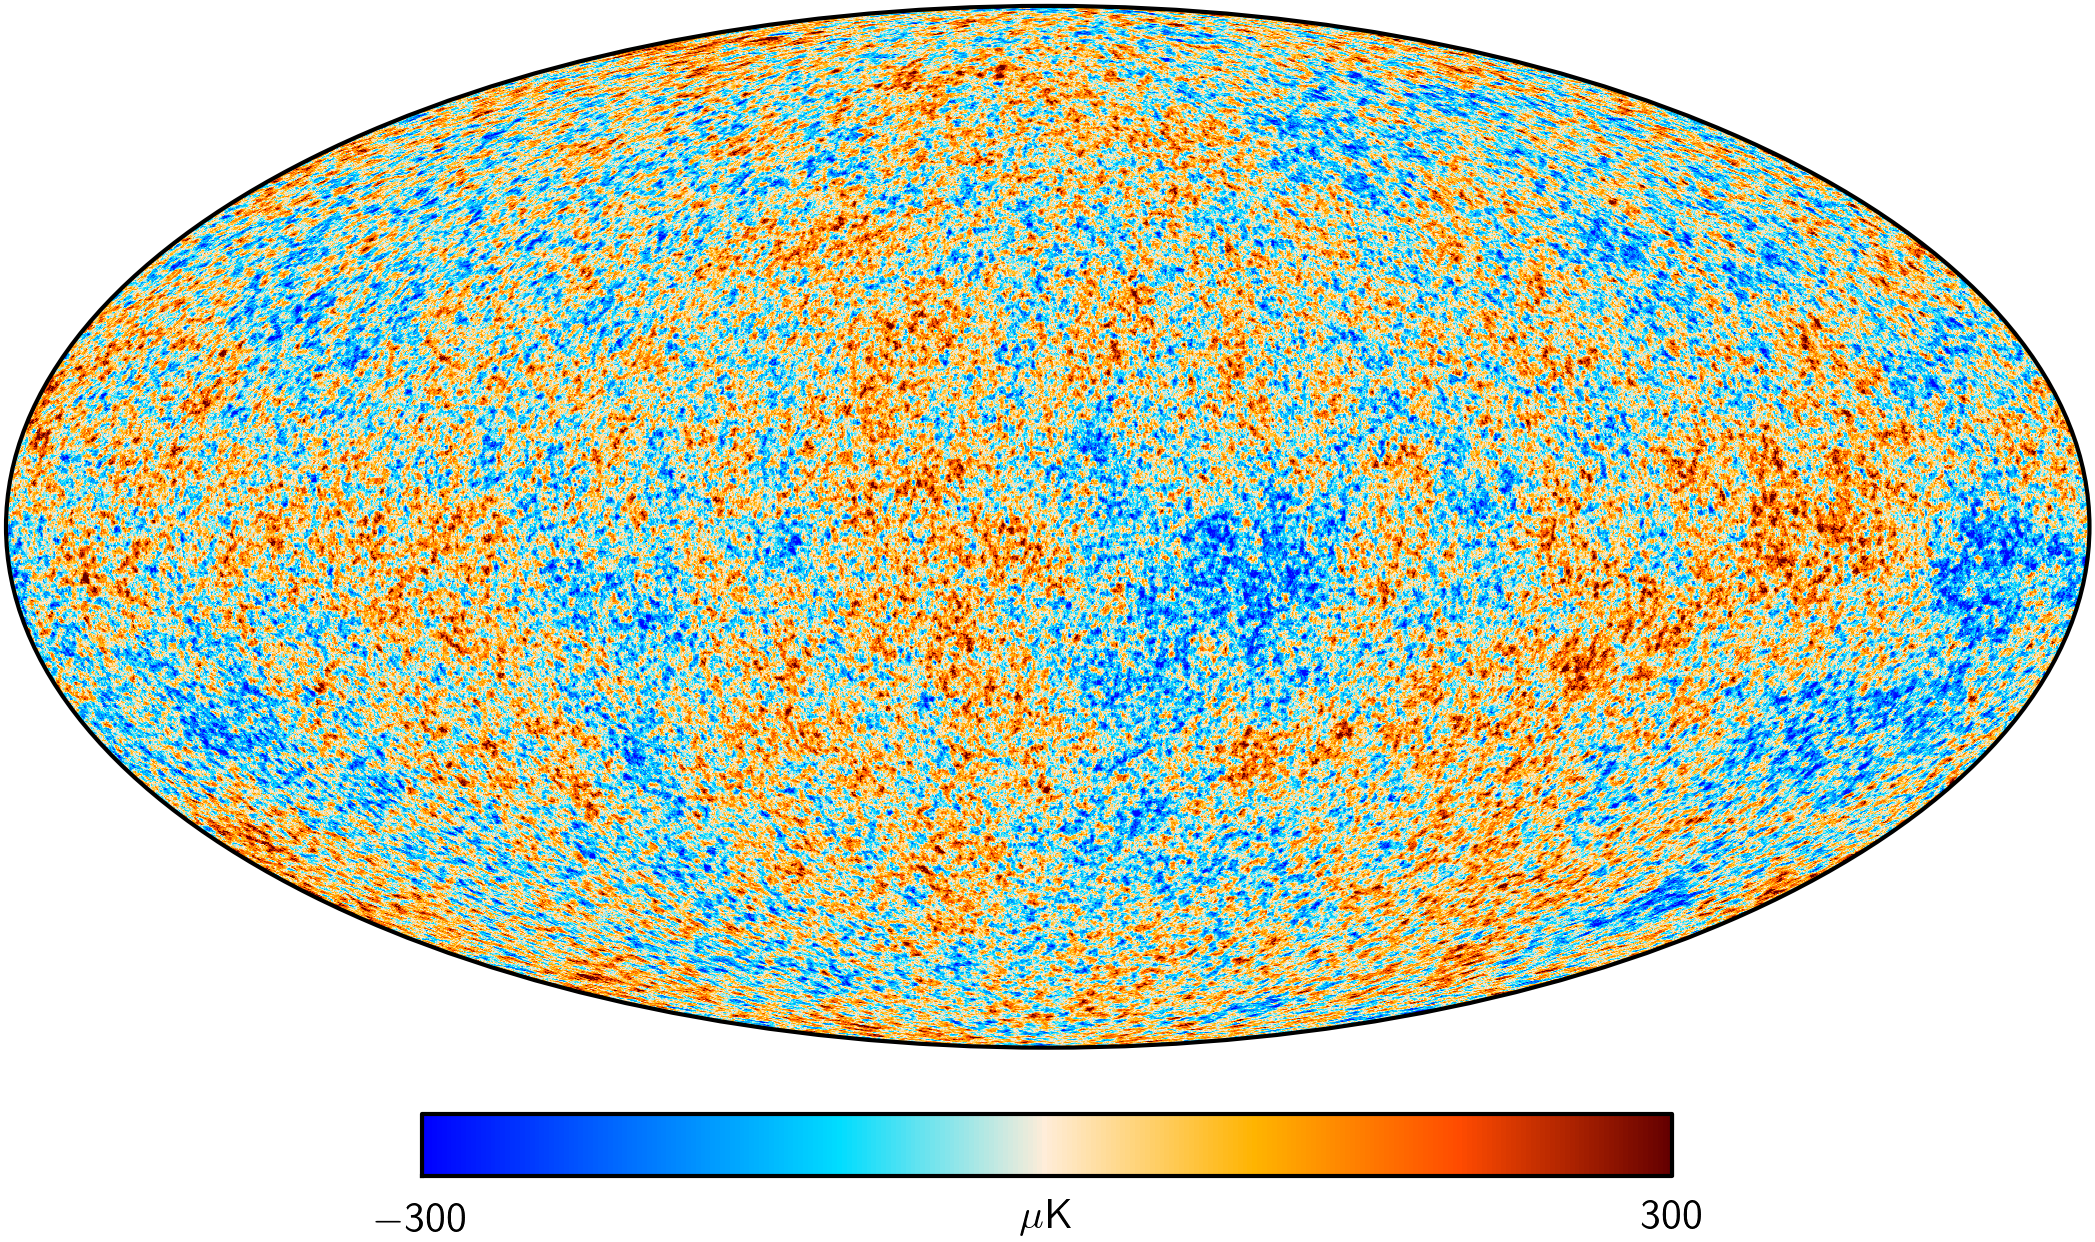
\includegraphics[width=\textwidth]{cmb/2015_SMICA_CMB.png}
\caption[A map of the CMB temperature anisotropies from the \textit{Planck} satellite.]
{
A map of the CMB temperature anisotropies using data from the \textit{Planck} satellite combined with other measurements~\autocite{Planck2015I}.
The color scale corresponds to the intensity deviations in units of temperature difference from the CMB mean temperature.
The angular resolution is 5'.
The CMB dipole due to our peculiar velocity has been removed, and galactic signals have been subtracted using observations at multiple frequencies, except for a small region in the galactic plane where the data has been generated randomly.
}
\label{fig:2015_SMICA_CMB}
\end{figure}

General relativity predicts the expansion rate of space, given its energy content.
On large scales, the expansion of a flat universe can be described by a single dimensionless parameter: the scale factor $a$.
The scale factor has increased monotonically over the history of the universe as we understand it, and is conventionally set to 1 today.
The evolution of the various components of the energy density depend in turn on the scale factor.
The energy density in matter goes as $\scalefactor^{-3}$, since the number of particles is conserved as the physical volume increases.
According to the standard model of cosmology, only 5\% of the current energy density of the universe is in the form of matter that is described by the standard model of particle physics.
An additional 25\% is in the form of cold dark matter that seems to not to interact electromagnetically.
Nearly all the remainder is in the form of dark energy, and observations are consistent with a cosmological constant that is independent of $a$.
The energy density in radiation, meaning photons and relativistic massive particles, goes as $\scalefactor^{-4}$; the additional factor of $\scalefactor$ arises from the cosmological redshift, or the stretching of each mode as space expands.
While radiation dominated the energy density of the early universe, it is negligible today.
The scale factor is closely related to the redshift
$\redshift
  =
  \wavelength_\mathrm{ob} / \wavelength_\mathrm{em} - 1
  =
  a^{-1} - 1$,
where $\wavelength_\mathrm{ob}$ and $\wavelength_\mathrm{em}$ are respectively the observed and emitted wavelengths of light.

Starting from the highest temperatures of which we have some experimental understanding, our observations support a picture of a universe that continually expands and cools while matter forms bound states of progressively lower energy and the components of radiation successively decouple.
The most widely studied models for even earlier times describe a period of nearly-instantaneous expansion called cosmic inflation~\autocite{Guth1981PRD}.
In order for such expansion to occur, inflationary models require adding one or more fields to the standard model of particle physics.
Since such fields are not observed today they must have decayed into more familiar fields at early times, and quantum fluctuations in the inflationary fields could have seeded the primordial density perturbations.
A generic prediction of inflation is a gravitational wave background that, if sufficiently large, would produce a characteristic imprint in the CMB.
Current experiments are searching for this imprint.

\begin{figure}[htb]
\centering
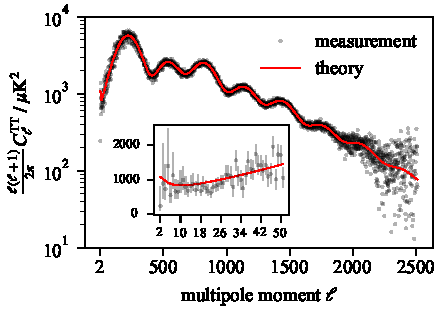
\includegraphics[width=\textwidth]{cmb/cmb_temperature_power_spectrum.pdf}
\caption[\textit{Planck} measurements of the CMB temperature power spectrum.]
{
\textit{Planck} measurements of the CMB temperature power spectrum.
The gray points are measured, unbinned, without error bars.
(One low outlier at high $\ell$ is not visible.)
The red curve is the prediction of the \textit{Planck} 2015 best-fit cosmology.
Measurements from ground-based experiments with larger primary apertures extend to much higher multipoles.
The inset shows the low-$\ell$ data on a linear scale, with error bars.
}
\label{fig:cmb_tt_power_spectrum}
\end{figure}

At very early times the temperature would have been too high for baryons to form, so this matter may have been in the form of the quark-gluon plasma that is studied through heavy-ion collisions in particle colliders~\autocite{Shuryak2017RMP}.
Around this time, some unknown process resulted in an excess of what we call matter over antimatter.
As the temperature decreased below that necessary for pair-production of baryons and anti-baryons, these mutually annihilated, leaving an excess of baryons.
When the temperature reached \SI{1}{MeV}, when the universe was about \SI{1}{s} old, the neutrinos decoupled.
Next, the electrons and positrons annihilated, leaving a universe that apparently contains no net charge and no antimatter.

By applying our understanding of nuclear physics to the conditions in the early universe, we can predict the relative abundances of  light nuclei, which would have formed when the temperature dropped to around \SI{0.1}{MeV}.
The predictions of this model of Big Bang nucleosynthesis agree well (except for $^7$Li) with current measurements of light elements corrected for processing in stars~\autocite{Cyburt2016RMP}.

\todo[inline]{Understand initial perturbation scales and their different evolution}
After the end of nucleosynthesis, the composition of the plasma did not change much until recombination began.
The initial perturbations were almost the same at all scales, but evolved differently.
In over-dense regions, increased gravitational attraction competed with increased radiation pressure from higher temperatures, and the plasma thus supported acoustic oscillations.
During this phase, when the temperature was of order \SI{10}{eV}, the energy density of radiation dropped below that of matter.


\subsection{During recombination}
\label{sec:cmb.physics.during}

Because of the large excess of photons over baryons, hydrogen did not form until the temperature had dropped to around \SI{0.25}{eV}, far below the hydrogen binding energy.
As recombination proceeded, over about 100,000 years, the universe became increasingly transparent.
Toward the end of recombination, the mean free path for photons became so large that they no longer scattered.
Perturbations in the primordial plasma were thus frozen in, and we observe them today in the CMB.
It turns out that the excess gravitational redshift for photons leaving over-dense regions outweighs the increased brightness due to the higher temperatures there, so colder regions observed today in the CMB correspond to hotter, higher density regions during recombination.

Cosmological models that assume isotropy and homogeneity can make only statistical predictions for fluctuations in the CMB.
Just as the spectral density is useful for characterizing time-stationary signals, the angular power spectrum of the CMB anisotropies is useful for comparing statistical predictions to measurements.
Since we measure the CMB on the celestial sphere, the angular power spectrum is computed using spherical harmonics characterized by the multipole moment $\ell$.
Power at a given $\ell$ corresponds to fluctuations at an angular scale of about $\SI{180}{\degree} / \ell$, which in turn corresponds to a length scale at recombination.
Figure~\ref{fig:cmb_tt_power_spectrum} shows the angular power spectrum of the CMB temperature anisotropies.
The first peak in the temperature power spectrum, at $\ell \sim 200$, or \SI{1}{\degree}, corresponds to the mode that reached its first maximum at recombination.
\todo[inline]{Understand acoustic peaks better}

\todo[inline]{CMB polarization fraction}
The CMB is also weakly linearly polarized, with the polarized intensity a few orders of magnitude more faint than the temperature anisotropies.
This linear polarization is produced by the density perturbations present during recombination: a quadrupole intensity perturbation oriented perpendicular to the line of sight produces net linear polarization along the line of sight due to elastic (Thomson) scattering.
The standard model predicts no circular polarization in the CMB, and measurements so far have produced only upper limits~\autocite{Nagy2017ApJ}.
The polarization of the CMB can thus be described by a pseudovector field on the celestial sphere.
Since there is no preferred orientation for the polarization field, it is useful to decompose it into an curl-free (even-parity) E-mode component and a divergence-free (odd-parity) B-mode component.
The density perturbations produce only E-mode polarization, which has been measured by many experiments.
The angular power spectrum of the E-modes measured by \textit{Planck} is shown in Figure~\ref{fig:cmb_polarization_power_spectrum}.

\begin{figure}[htb]
\centering
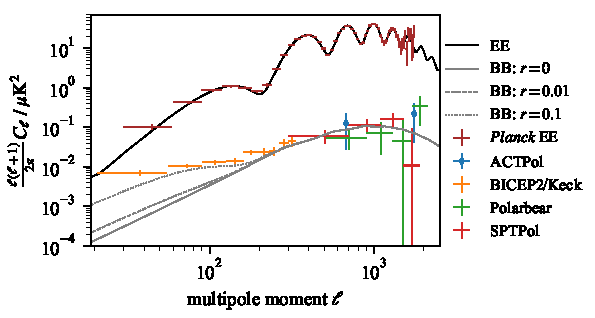
\includegraphics[width=\textwidth]{cmb/cmb_polarization_power_spectrum.pdf}
\caption[Recent measurements of the CMB E-mode and B-mode power spectra.]
{Recent measurements of the CMB E-mode and B-mode power spectra.
The E-mode data are from the 2015 \textit{Planck} release.
(Data at the lowest and highest multipoles, where the error bars are large, are not shown.)
The B-mode data were released by ACTPol~\autocite{ACTPol2017JCAP},
BICEP2/Keck Array~\autocite{BK2016PRL},
Polarbear~\autocite{Polarbear2017ApJ}, 
and SPTPol~\autocite{SPTPol2015ApJ}.
Data sets binned in other units have been converted to the displayed units using the center bin value, which is only approximately correct.
Where bins widths were available, these are shown by the horizontal bars; otherwise, a single point shows the center bin.
The theory curves were calculated with CAMB~\autocite{CAMB}: the solid black line and solid gray lines use the Planck 2015 best-fit cosmology~\autocite{Planck2015XIII}, and the dashed and dotted gray lines also include a nonzero tensor-to-scalar ratio $r$.}
\label{fig:cmb_polarization_power_spectrum}
\end{figure}

Gravitational waves decay as the universe expands, and any that were produced by inflation would be undetectable today.
However, gravitational waves present during recombination would have imprinted a primordial B-mode signature in the CMB.
\todo[inline]{Understand exact definitions of $r$}
The amplitude of these perturbations is commonly modeled by adding one parameter, the tensor-to-scalar ratio $r$, to the standard model.
Figure~\ref{fig:cmb_polarization_power_spectrum} shows the angular power spectrum of the B-modes measured by recent experiments as well as theoretical predictions for several values of $r$.
Larger values of $r$ correspond to larger signals in the B-mode power spectrum, and this primordial signal could be measurable at large angular scales.
However, the amplitude of the inflationary signal is not well-constrained by theory, and could be too small to measure even if inflation occurred.
The data points from the BICEP2 and Keck Array experiments show an excess B-mode signal at low multipoles, but this signal is dominated by galactic dust~\autocite{BKP2015PRL}.
The current upper limit from CMB data is $r < 0.09$ at 95\% confidence~\autocite{BK2016PRL}.


\subsection{After recombination}
\label{sec:cmb.physics.after}

After recombination, the baryons are almost entirely in the form of neutral hydrogen and helium.
The CMB photons thus pass freely through the universe as the over-dense regions slowly collapse into the structure we see today.
Although the CMB no longer exchanges much energy with matter, the gravitational redshift turns out to preserve the shape of the black body curve, and the CMB remains a nearly-perfect black body at a temperature inversely proportional to the scale factor.

Today, the CMB temperature is reduced by a factor of the redshift at recombination, approximately 1100, to $\temperature_\mathrm{CMB} = \SI{2.7255}{K} \pm \SI{0.0006}{K}$~\autocite{Fixsen2009ApJ}.
Figure~\ref{fig:firas_monopole_spectrum} shows the spectrum of the CMB measured by the FIRAS instrument on the COBE satellite.
For a black body at the CMB temperature the peak of the brightness spectral density occurs near frequency $\foptical = \SI{160}{GHz}$, and the occupancy
$\photonoccupancy(\foptical) = [\exp(\planck \foptical / \kb \temperature_\mathrm{CMB}) - 1]^{-1}$ drops below 1 above $\foptical \approx \SI{40}{GHz}$.

\begin{figure}[tb]
\centering
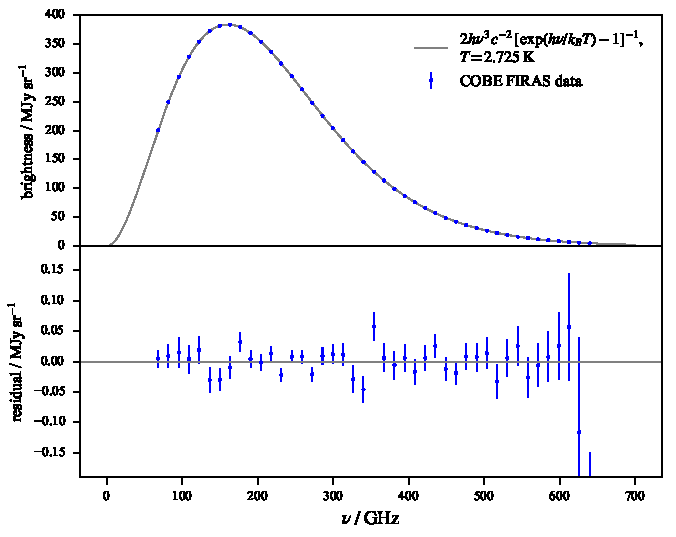
\includegraphics[width=\textwidth]{cmb/firas_monopole_spectrum.pdf}
\caption[The CMB monopole spectrum from FIRAS on COBE.]
{
The CMB monopole spectrum from the FIRAS instrument on the COBE satellite~\autocite{Fixsen1996ApJ, Fixsen2002ApJ}.
\textbf{(Upper)} The blue points are measured (with error bars that are too small to be visible), and the gray line is the black body curve given in the legend.
\textbf{(Lower)} Residuals from the upper panel.
The blue points are the measured data minus the model.
}
\label{fig:firas_monopole_spectrum}
\end{figure}

The CMB we detect today originates from a distant last-scattering surface, and it has been altered during the subsequent history of the universe.
CMB photons do not interact much during the so-called cosmic dark ages, until the first stars form and begin to emit photons that have sufficient energy to reionize the neutral gases.
\todo[inline]{Redshift of reionization.}
However, even after reionization, only a small fraction of CMB photons scatter.
\todo[inline]{Effect of reionization on the CMB.}
Weak gravitational lensing converts E-mode polarization into B-mode polarization at an amplitude that can be calculated from the known evolution of the matter distribution since recombination. 
In Figure~\ref{fig:cmb_polarization_power_spectrum}, the B-mode measurements at smaller angular scales are roughly consistent with the expected amplitude due to lensing.

\todo[inline]{Incorporate material on LCDM parameters.}
\begin{comment}
\subsection{The standard model of cosmology}
\label{sec:cmb.physics.cosmology}

Most of the parameters of the standard model of cosmology relate to fundamental gaps in our understanding.
The age of the universe and the spectral index of primordial fluctuations describe a universe that has a finite age and began in a hot, dense, and slightly inhomogeneous state.
The spectral index quantifies the amplitude of these primordial fluctuations in the density and temperature as a function of their size initial, but the mechanism that seeded these initial conditions is uncertain.
Two parameters describe the fractional energy content of the universe in baryons (the cosmological term that encompasses all hadron and lepton matter) and in cold dark matter (CDM), which are respectively about 5\% and 25\% of the total.
Measurements on widely-differing scales provide strong evidence for a particle that does not interact electromagnetically, but such a particle is not described by the standard model of particle physics and has not been directly detected.
Even the prosaic baryon fraction relates to the mystery of the excess of matter over antimatter that presumably produced the initial matter and photon content through annihilation.
The remaining energy content, about 70\% of the total, is apparently in the form of dark energy, modeled as a cosmological constant $\Lambda$, which causes the accelerating expansion of the universe.
One parameter relates to the curvature of the universe on large scales: current measurements are consistent with the universe being flat, but there is no known reason for this to be the case.
The final parameter, the optical depth to reionization, simply describes the opacity of the universe to CMB photons.
Fortunately, even the recent universe is fairly transparent, which has allowed us to learn much of what we know about cosmology.
\end{comment}


\section{Experiment}
\label{sec:cmb.experiment}

\subsection{Goals}
\label{cmb.experiment.goals}

Current CMB mapping experiments focus on polarization in order to improve on the measurements shown in Figure~\ref{fig:cmb_polarization_power_spectrum}.
A major goal is to search for the signature of primordial B-modes produced by inflation, which would give valuable information about physics at higher energies than we can currently probe.
\todo[inline]{Understand neutrino mass constraints}
Another major experimental goal is to constrain the sum of the masses of all neutrino species, which is possible because all of the constituents of the primordial plasma affect the CMB~\autocite{CMBS4ScienceBook}.
By contrast, neutrino oscillation experiments are sensitive to differences in the squares of the neutrino masses.

Since the CMB photons traverse nearly the entire visible universe, signals from closer sources are called foregrounds.
Polarized galactic foregrounds are brighter than the CMB polarization at most frequencies, and this is a major experimental challenge.
Overcoming it requires measurements in different frequency bands around the CMB peak in order to model and subtract the foreground signals.
The multichroic pixels described in Chapter~\ref{chp:multichroic} can each simultaneously measure two linear polarization states in two spectral bands.


\subsection{Signals}
\label{sec:cmb.experiment.signals}

In a typical band containing the \SI{160}{GHz} peak of the CMB spectrum, a detector on a space-based instrument with very cold optics would absorb about \SI{0.1}{pW}, or \SI{e9}{photons/s}.
The load in a ground-based instrument might be three orders of magnitude greater because the atmosphere is emissive in the millimeter-wave region and is much hotter than the CMB.
In both cases, the time between photon arrivals is much less than the response time of the detector, which thus measures only the average photon flux.

The fractional anisotropies of the CMB intensity are of order \num{e-5}, so the linearity and dynamic range requirements will be set by other, larger signals.
Experiments may observe bright calibrators, such as planets or artificial linearly polarized sources used to measure detector polarization angles.
Ground-based experiments must also contend with atmospheric fluctuations: even at the dry, high-altitude sites that are used for ground-based CMB observations, the atmosphere is much brighter than the CMB, with a typical effective Rayleigh-Jeans temperature of several tens of kelvin.

In principle, a CMB telescope could point at a particular location on the sky, average down the noise to the desired level, then move to another location.
In practice, this is not done because slow drifts in the instrument response produce systematic effects that are difficult to correct. 
Thus, a telescope typically scans repeatedly over the same 
patch of sky and revisits any given point many times.
(For polarimetry, it is useful to scan the same point on the sky from different instrument orientations, as this tends to average down some systematic errors.)
To reduce the demands on detector linearity, ground-based instruments often perform such scans at a constant elevation to maintain a constant load from the atmosphere.

Beams in existing instruments are designed to be approximately Gaussian with an angular diameter from about \SI{1}{\arcminute}~\autocite{ACT2011ApJS} to \SI{30}{\arcminute}~\autocite{BICEP2II2014ApJ},
typically limited by diffraction at the primary aperture.
The beam acts as a filter: information on scales much smaller then the beam is averaged out.
As a detector scans across the sky, modes at different angular scales are modulated at different frequencies in the time-ordered data.
A mode with angular wavelength $\lambda$ will appear in the time-ordered data of a detector scanning the sky with angular velocity $\dot{\theta}$ at audio frequency
$\faudio = \dot{\theta} / \lambda$, and the beam will create a low-pass filter in the frequency domain.
To avoid the difficulty of deconvolving the detector response from the time-ordered data, the detector bandwidth should be significantly greater than the bandwidth of this filter.

CMB polarimeters may use a modulator to separate the intensity signal from the fainter polarization signal in the frequency domain.
For example, a spinning half-wave plate will cause a constant polarization signal to appear in a power detector, or ``square-law'' detector, at four times its rotation frequency.
Modulation of the polarization at \SI{10}{Hz} has been demonstrated to work in a ground-based experiment~\autocite{Kusaka2014RSI},
and a prototype superconducting bearing system exists that could modulate at \SI{40}{Hz} or more~\autocite{Johnson2017RSI}.
The spectral density of detector data is typically red below a ``knee'' frequency at \SIrange{0.1}{10}{Hz} due to fluctuations in the atmospheric signal or in the detector system itself.
Thus, modulation may shift the polarization signal to a frequency band where the data is less contaminated by red noise.

The CMB anisotropies of current interest are faint in the sense that significant time may be needed to measure them, even when the only noise is due to the randomness of photon arrival times.
Existing detectors have sensitivity near this photon-noise limit, even in space, where the CMB may be the main contribution to the total detected power.


\subsection{Detectors}
\label{sec:cmb.experiment.detectors}

We can extract criteria for CMB detectors from the preceding discussion.
The detectors must be sufficiently linear to not distort the measured signals; the exact requirement will depend on the calibration strategy, and nonlinearity may be mitigated by injecting calibration signals.
The ideal noise level is less than the photon noise under the expected optical load, which depends on the instrument design and location.
The detector noise requirements are progressively more stringent for ground-based, balloon-borne, and space-based instruments.
The detector bandwidth should be sufficiently large to accommodate all signals of interest without excessive distortion.
For an instrument without polarization modulation that scans slowly, a bandwidth of \SI{10}{Hz} or less might be sufficient.
Using either a continuous calibration signal or a fast polarization modulator might increase the bandwidth requirement by an order of magnitude.

The detector technologies that have shown competitive sensitivity for CMB experiments all operate at temperatures below about \SI{1}{K}.
For the cryogenic requirements, and thus the cost, to be manageable, it must be possible to read out many of these cryogenic detectors using a small number of wires.
Techniques in use include time-division multiplexing, in which many detectors on a common wire are interrogated sequentially using switches, and frequency-division multiplexing, in which many detectors on a common wire are interrogated simultaneously using signals at unique frequencies that are somehow filtered so that each signal interacts with only one detector.

When the noise added by a detector is less than the photon noise, the only way to significantly increase the mapping speed of a detector array is to increase the number of detectors.
Most current suborbital experiments use transition-edge sensor (TES) bolometers.
The motivation for the work done in this thesis is that the kinetic inductance detector (KID), which naturally lends itself to frequency multiplexing, may offer an easier route to deploying larger arrays.
Current ground-based experiments use thousands of detectors, and proposed experiments will use tens or hundreds of thousands of detectors~\autocite{CMBS4TechnologyBook}.


\chapter{Kinetic inductance detectors: basic theory}
\label{chp:theory}

A KID is a superconducting thin-film microresonator in which the resonator itself is a detector~\autocite{Day2003Nature}.
The detection is performed by using a microwave tone at the KID resonance frequency to measure changes in the electrodynamic response of the film, which is altered by deposited energy.
Figure~\ref{fig:multiplexed_mkids_v1} shows the basic multiplexing concept.
Each detector has a unique resonance frequency, and electronics similar to software-defined radio are able generate and analyze hundreds to thousands of tones simultaneously, allowing many detectors to be multiplexed.

\begin{figure}[htb]
\centering
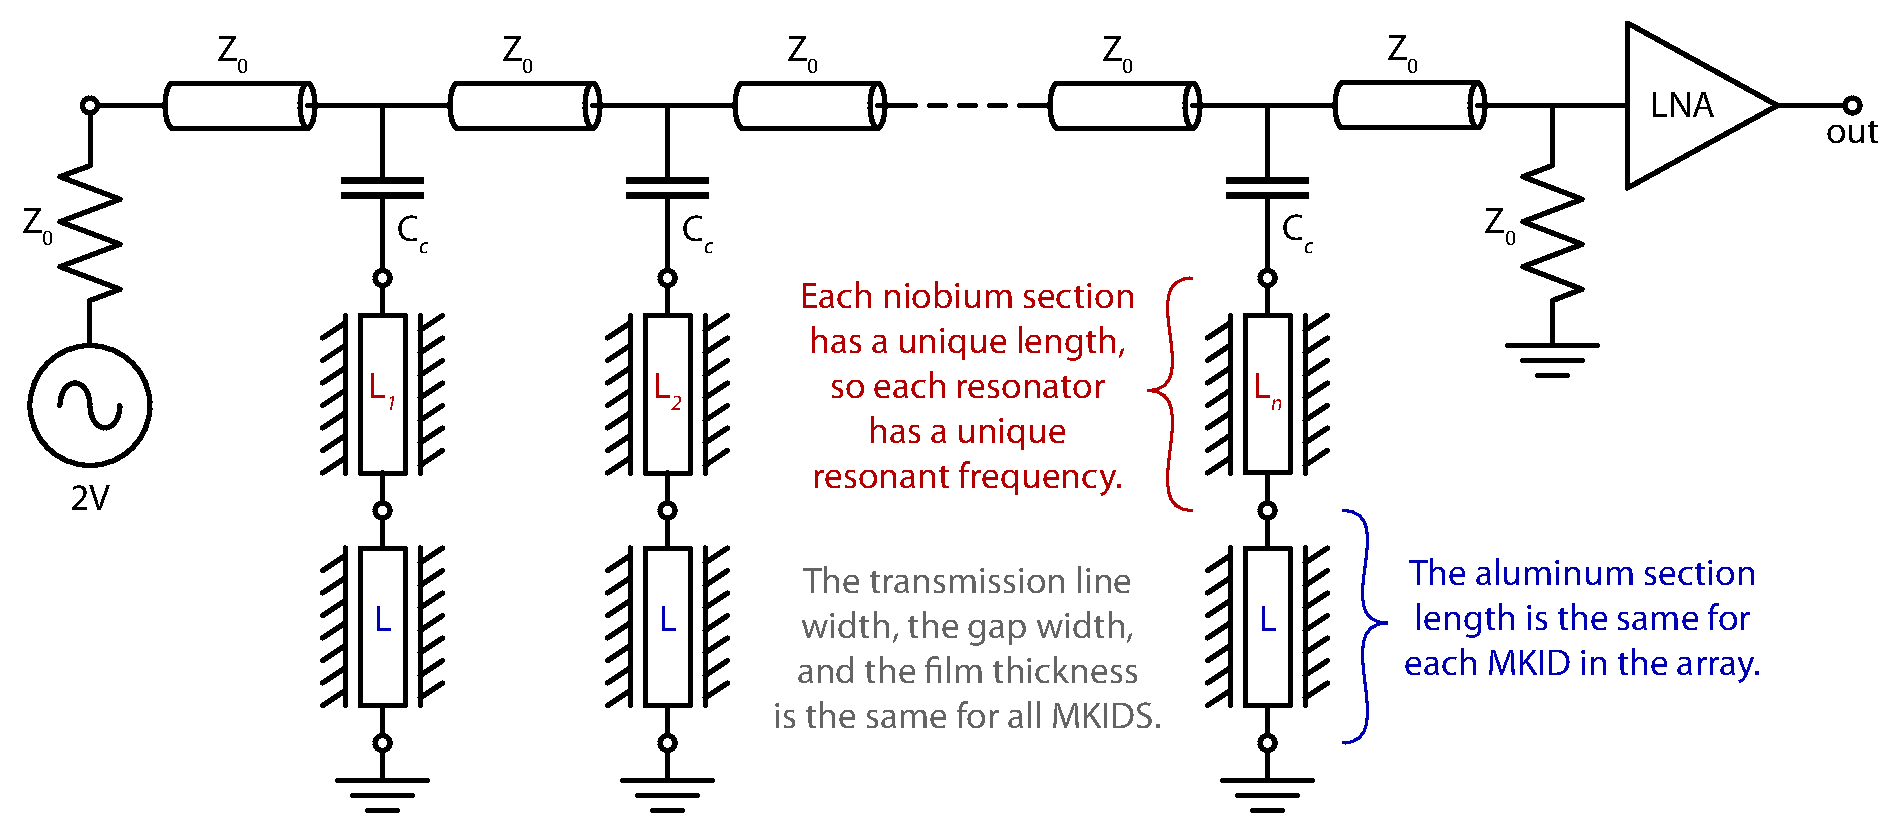
\includegraphics[width=0.8\textwidth]{theory/multiplexed_mkids_v1.pdf}
\caption[A schematic that shows how KIDs are read out and multiplexed.]
{
A schematic that shows how KIDs are read out and multiplexed.
The annotation refers specifically to the KIDs that are discussed in Chapter~\ref{chp:multichroic}, which are made from aluminum and niobium.
The tones are generated at left, propagate past the detectors, and are amplified at right by the low-noise amplifier (LNA).
}
\label{fig:multiplexed_mkids_v1}
\end{figure}

Figure~\ref{fig:introduction_resonator_amplitude_phase} shows how a KID responds to an increase in illumination: the resonance frequency decreases, and the internal dissipation increases.
The changes shown in the plot were due to a change in the temperature of a black body load that illuminated the detectors.

\begin{figure}[htb]
\centering
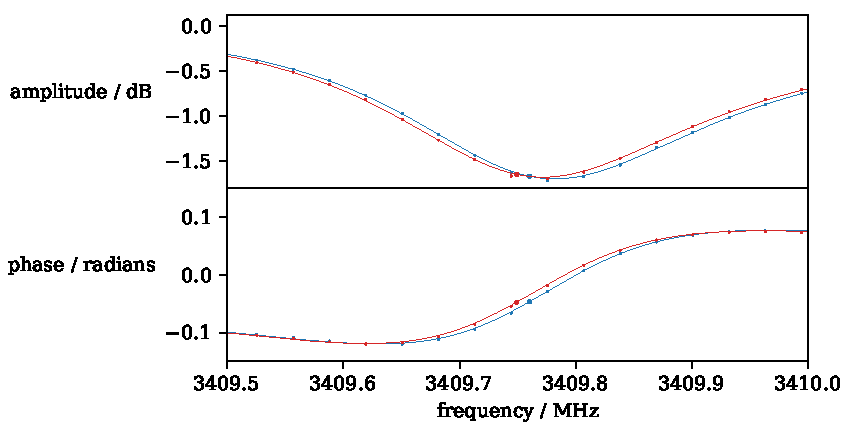
\includegraphics[width=0.7\textwidth]{theory/introduction_resonator_amplitude_phase.pdf}
\caption[The amplitude and phase of the forward transmission past a resonator, versus frequency.]
{
The amplitude and phase of the forward transmission past a resonator, plotted versus frequency, taken at two different levels of illumination from a beam-filling black body source.
The blue (red) points were taken with the source at \SI{3.3}{K} (\SI{5}{K}).
The small points are the data, the lines are a fit to a resonator model, and the large points mark the resonance frequencies extracted from the fits.
}
\label{fig:introduction_resonator_amplitude_phase}
\end{figure}

In this chapter I introduce the theory that is necessary to understand the response of a KID to light.
Section~\ref{sec:theory.ground_state} contains a quick introduction to the necessary elements of the BCS theory of superconductivity and the superconducting ground state.
In Section~\ref{sec:theory.quasiparticle}, I discuss the generation, scattering, decay, and diffusion of the quasiparticle excitations of a superconductor.
In Section~\ref{sec:theory.electrodynamics}, I discuss superconductor electrodynamics, focusing on the effect of the quasiparticles.
In Section~\ref{sec:theory.perturbation}, I introduce a framework for describing the non-equilibrium state of a superconducting thin film as a small perturbation to the ground state.
In Section~\ref{sec:theory.qpnumber}, I introduce a simplified description of the film in terms of only the total number of quasiparticles, then use this model to motivate and solve the equations that describe the dynamics of the quasiparticle system.
In Section~\ref{sec:theory.resonator}, I discuss a generic model for a shunt-coupled resonator and use it to describe the lumped-element and transmission-line resonators used for the KIDs in this thesis.
In Section~\ref{sec:theory.response}, I use the results from previous sections to derive the response equations for a detector, starting with the absorption of light and ending with the electrical signal that is recorded by the electronics.

\section{The BCS theory and the ground state }
\label{sec:theory.ground_state}

\subsection{The Cooper pair condensate}
\label{sec:theory.ground_state.condensate}

\todo[inline]{Re-read Tinkham and update.}
In the Bardeen-Cooper-Schrieffer (BCS) theory of superconductivity~\autocite{BCS1957PRL, BCS1957PR}, the superconducting ground state can be described in terms of individual-electron (Bloch) states occupied in pairs with opposite momentum and spin, called Cooper pairs~\autocite{Cooper1956PRL}.
These Cooper pairs form due to a phonon-mediated attractive potential $\bcspotential$ between electrons that are within the Debye energy $\phononenergy_\debye$ of the Fermi energy.
The coherence length
$\coherencelength \sim \hbar \velocity_\fermi / \kb \tc$,
where $\velocity_\fermi$ is the Fermi velocity and $\tc$ is the critical temperature for the superconducting phase, corresponds to the minimum size of a Cooper pair as dictated by the uncertainty principle.
For elemental superconductors the coherence length is much greater than the mean spacing between conduction electrons.
While it is more accurate to think of correlations extending over a distance $\coherencelength$, a naive model of the pair condensate is sufficient for the calculations in this thesis.

In a normal metal at temperature $\temperature = 0$, by definition, no states with energy greater than the Fermi energy $\blochenergy_\fermi$ are occupied.
However, in a superconducting metal, even at $\temperature = 0$, some states within an energy range approximately $\kb \tc$ above the Fermi energy remain populated.
The increase in kinetic energy compared to the normal state is outweighed by the decrease in potential energy due to the pairing.

One of the most striking features of the transition to the superconducting state is the Meissner effect, in which, as the temperature is reduced below $\tc$, a screening supercurrent develops to expel any magnetic field from the interior of a bulk superconductor.
This screening is quantified by the penetration depth $\penetrationdepth$, which is the distance from a surface over which the screening supercurrent causes magnetic fields to decay in the bulk.
In the phenomenological London theory, developed long before the BCS theory, the penetration depth at zero temperature is
\begin{equation}
\penetrationdepth_\mathrm{L}
  =
  \left( \frac{\lsvac m_\mathrm{s}}{\impvac n_\mathrm{s} q_\mathrm{s}^2}
  \right)^{1/2},
\end{equation}
where $\lsvac$ is the speed of light in vacuum, $\impvac$ is the impedance of vacuum, and $m_\mathrm{s}$, $n_\mathrm{s}$, and $q_\mathrm{s}$ are respectively the mass, density, and charge of the superconducting carriers.
The aluminum films used for the detectors discussed in this thesis are \SIrange{10}{50}{nm} thick, while the bulk penetration depth for aluminum at low temperature and low frequency is about \SI{50}{nm}~\autocite{Faber1955PRS, Biondi1959bPR}, so the fields completely enter these films. 
The penetration depth is closely related to the reactive part of the superconductor's surface impedance $\impedance_\surface$, discussed in Section~\ref{sec:theory.electrodynamics.surface_impedance} below.

\todo[inline]{Understand time-varying field screening.}
%As in the normal metal, static electric fields are screened over atomic-scale lengths.

In a BCS superconductor below $\tc$, there is a minimum energy $\gap$, called the gap energy, for excitations from the ground state.
These excitations are important for the electrodynamic behavior of a KID, and are discussed in detail later.
In the in the weak-coupling limit of BCS theory, where
$\ssdos \ucvolume \bcspotential \ll 1$,
the critical temperature $\tc$ is proportional to the zero temperature gap energy $\gap_\zerotemp$.
Here, $\ssdos$ is the single spin density of states at the Fermi energy and $\ucvolume$ is the volume of a unit cell.
The relationship is $\gap_\zerotemp = 1.76 \, \kb \tc$, and the numerical factor is accurate to about 20\% in actual elemental superconductors~\autocite{Tinkham2004}.


\subsection{Fiducial parameters}
\label{sec:theory.ground_state.fiducial}

In our current experimental setup we measure the transition temperature either by observing the change in film resistance using a standard four-wire scheme or by observing changes in microwave transmission through the transmission line on a chip containing resonators.
In \SIrange{10}{50}{nm} thick aluminum films we typically measure $\tc$ slightly elevated from the bulk value of \SI{1.2}{K} by \SIrange{0.1}{0.2}{K}, in agreement with other measurements of thin aluminum films~\autocite{Townsend1972PRB}.
Although we are not yet able to directly measure $\gap$, measurements of the gap in thin aluminum films have also shown enhancement above the bulk value~\autocite{Court2008SUST}, and in the absence of a gap measurement we typically assume that the BCS relation remains valid.
Note that some relevant quantities vary exponentially with the ratio of the gap to the temperature, so a small uncertainty in the gap energy may lead to a much larger uncertainty in predictions of such quantities.

As shown in Table~\ref{tab:energies}, the two types of KIDs I discuss here have very different typical resonance frequencies.
In both cases, $\planck \freadout / \gap \ll 1$.
If $\temperature_\bath$ is the bath temperature of the detectors, then for the single-polarization lumped-element KIDs $\planck \freadout_\singlepol / \kb \temperature_\bath \ll 1$, while for the multichroic co-planar waveguide KIDs $\planck \freadout_\multichroic / \kb \temperature_\bath \approx 1$.
This distinction is not practically important for the readout photon occupancy, because the readout power is always sufficiently high to produce an occupancy much greater than one.

\begin{table}[htb]
\centering
\caption
[Fiducial energies, temperatures, and frequencies.]
{
Fiducial energies, temperatures, and frequencies:
$\tc$ is close to the critical temperature we typically measure in aluminum films;
$\temperature_\bath$ is a typical bath temperature; 
$\freadout_\singlepol$ is a typical resonance frequency for the single-polarization lumped-element KIDs used in experiments discussed in Chapters~\ref{chp:loss}~and~\ref{chp:sensitivity};
$\freadout_\multichroic$ is a typical resonance frequency for the multichroic CPW KIDs discussed in Chapter~\ref{chp:multichroic}.
I use these values for numerical estimates, including the slightly elevated gap and critical temperature.
}
\renewcommand{\arraystretch}{1.2}
\begin{tabular}{c S S S S}
\toprule
Parameter & \si{J} & \si{\micro eV} & \si{GHz} & \si{K} \\
\midrule
$\gap_\zerotemp$ & 3.16e-23 & 197.16 & 47.67 & 2.288 \\
$\tc$ & 1.79e-23 & 112.03 & 27.09 & 1.300 \\
$\freadout_\multichroic$ & 1.99e-24 & 12.41 & 3.00 & 0.144 \\
$\temperature_\bath$ & 1.79e-24 & 11.20 & 2.71 & 0.130 \\
$\freadout_\singlepol$ & 6.63e-26 & 0.41 & 0.10 & 0.005 \\
\bottomrule
\end{tabular}
\label{tab:energies}
\end{table}

KIDs have been made from numerous materials, some of which are not well-described by the BCS theory.
However, the KIDs discussed in this work are made either from only aluminum or from both aluminum and niobium, both of which are BCS superconductors.
Throughout this thesis, when making numerical estimates, I use typical material parameters for aluminum and niobium given in Table~\ref{tab:materials} along with the fiducial values given in Table~\ref{tab:energies}, including the slightly elevated values of $\tc$ and $\gap$ that we typically measure.
These should give reasonable descriptions of the detectors we have tested.

\todo[inline]{Check N0 for niobium and understand values given by Kaplan et al.}
\begin{table}[htb]
\centering
\caption[Parameters of superconducting metals used in this thesis.]
{
Parameters of superconducting metals used in this thesis.
See Table~\ref{tab:notation.condensed_matter} for the symbol definitions.
Values are from \textcite{Kaplan1976PRB} except where noted.
}
\renewcommand{\arraystretch}{1.2}
\begin{tabular}{c c c c}
\toprule
Parameter & Unit & Aluminum & Niobium \\
\midrule
$\tc$ (bulk) & \si{K} & 1.19 & 9.2 \\
%$\gap_\zerotemp$ & {} & {} & {} \\ 
$\ssdos$ & \si{eV^{-1}.\micro\meter^{-3}} & \num{1.74e10}~\autocite{Thomas2015SUST} & \num{8.52e10}~\autocite{Jani1988PRB} \\
$\electronphonontime$ & \si{ns} & 438 & 0.149 \\
\bottomrule
\end{tabular}
\label{tab:materials}
\end{table}

\subsection{Radiation detection using superconductors}
\label{sec:theory.ground_state.detection}

For a KID absorbing pair-breaking radiation, the cutoff (lowest detectable) frequency is
\begin{equation}
\foptical_\cutoff 
  =
  2 \gap / \planck
  \approx
  3.5 \, \kb \tc / \planck
  \approx
  \SI{74}{GHz} \left( \tc / \SI{1}{K} \right).
\end{equation}
To minimize the rate of thermal excitations, KIDs must be operated at a low bath temperature.
If $\temperature_\bath$ is the practically achievable bath temperature for a large detector array designed to detect photons with frequency $\foptical$, the superconducting energy gap must satisfy
\begin{equation}
\planck \foptical / 2
  >
  \gap
  \gg
  \kb \temperature_\bath.
\end{equation}
Fortunately, this is currently possible over at least part of the frequency range relevant for CMB observations.
Aluminum can be used to detect pair-breaking photons with frequencies above
$\foptical_\cutoff \approx \SI{100}{GHz}$.
Refrigeration using adiabatic demagnetization or helium dilution allows for cooling of large arrays to temperatures
$\temperature_\bath \approx \SI{0.1}{K} \sim \tc / 10$,
sufficiently low that thermal excitations are negligible.
This allows KIDs to achieve, in principle, the fundamental sensitivity limit set by the statistics of photon arrival.

\section{Quasiparticle excitations}
\label{sec:theory.quasiparticle}

\subsection{The quasiparticle density of states}
\label{sec:theory.quasiparticle.dos}

The quasiparticle excitations that are orthogonal to the ground state are neither lone electron nor hole excitations, but are superpositions of excitations on both sides of the Fermi surface.
These excitations are commonly called Bogoliubov quasiparticles, and I refer to them simply as quasiparticles.
They have spin $1 / 2$ and thus obey Fermi statistics.
Their canonical decay mechanism is to rejoin the condensate by recombining in pairs to form a Cooper pair and emitting a phonon.
Other decay channels are discussed below.

Because of the gap, there are no low-energy states into which the constituents of the Cooper pairs can individually scatter, and a supercurrent can thus flow with no resistance, at least at zero frequency.
However, like the conduction electrons of the normal metal, the quasiparticles experience lossy scattering.
Thus, the conductivity at nonzero frequencies, while typically much higher than in even an excellent normal conductor, is finite.
A KID detects radiation essentially by measuring these excitations through their effect on the surface impedance of the superconductor at microwave frequencies.

\todo[inline]{update after reading AM}
The energy of a Bloch state with wavevector $\vwvec$ is
$\blochenergy_{\vwvec} = \hbar^2 \wvec^2 / 2 \mass$
for an electron mass $\mass$.
If $\blochenergyf_{\vwvec} = \blochenergy_{\vwvec} - \blochenergy_\fermi$ is the same energy relative to the Fermi energy $\blochenergy_\fermi$, then the energy of a quasiparticle with wavevector $\vwvec$ is
\begin{equation}
\energy_{\vwvec}
  =
  \left( \blochenergyf_{\vwvec}^2 + \gap^2 \right)^{1/2},
\label{eqn:qpenergy}
\end{equation}
which is positive for excitations on both the ``electron'' branch outside the Fermi surface, with $\blochenergyf > 0$, and the ``hole'' branch inside the Fermi surface, with $\blochenergyf < 0$.
This relationship between the Bloch state energy and the quasiparticle energy is plotted in Figure~\ref{fig:quasiparticle_energy_and_density_of_states}(a).

\todo[inline]{Recreate BCS figure.}
\begin{figure}[htb]
\centering
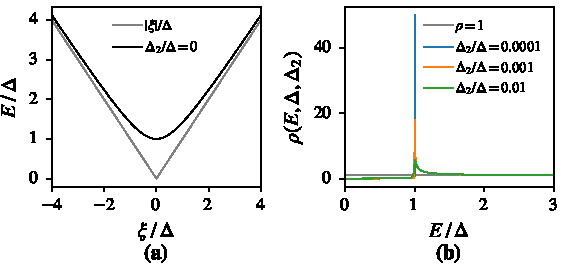
\includegraphics[width=\textwidth]{theory/quasiparticle_energy_and_density_of_states.pdf}
\caption
[The quasiparticle energy and density of states.]
{
\textbf{(a)}
The BCS quasiparticle energy $\energy$ versus the Bloch state energy $\blochenergyf$ in units of the gap.
Here, the Fermi energy is at $\blochenergyf = 0$.
\textbf{(b)}
The reduced density of states $\qprdos$ versus the quasiparticle energy $\energy$ in units of the gap.
For display, the three density of states curves have all been broadened by adding small imaginary parts to the gap:
$\gap \rightarrow \gap - \I \mitrovic$.
The gray horizontal line shows $\qprdos = 1$, which is the asymptotic value at high $\energy$.
%(If the corresponding energies were plotted in (a), they would have very narrow dips near $\blochenergyf = 0$ down to a minimum near $\energy / \gap = 0$.)
}
\label{fig:quasiparticle_energy_and_density_of_states}
\end{figure}

The range of energies involved forming the superconducting state is small compared to the Fermi energy.
Because the normal metal density of states does not change much over this range of energies, it is conventional to take it to be constant and to define $\ssdos$ to be the number of electron states of one spin per unit energy per unit volume at the Fermi energy.
The BCS density of states arises from the relationship between the quasiparticle energy $\energy$ and the Bloch energy $\blochenergyf$:
\begin{equation}
\dd{\energy}
  =
  \dd{\left( \blochenergyf^2 + \gap^2 \right)^{1/2}}
  =
  \frac{\blochenergyf \dd{\blochenergyf}}{\left( \blochenergyf^2 + \gap^2 \right)^{1/2}},
\end{equation}
so
\begin{equation}
\dd{\blochenergyf}
  =
  \frac{\energy \dd{\energy}}{\left(\energy^2 - \gap^2 \right)^{1/2}}.
\end{equation}
The density of quasiparticle states is thus
\begin{equation}
\supssdos(\energy)
  =
  \ssdos \dv{\blochenergyf}{\energy}
  =
  \ssdos \frac{\energy}{(\energy^2 - \gap^2)^{1/2}}
  \equiv
  \ssdos \qprdos(\energy),
\label{eqn:supssdos}
\end{equation}
where $\qprdos$ is the \textit{normalized} (or \textit{reduced}) density of states.
There is a one-to-one correspondence between the Bloch states and the quasiparticle states, so the total number of states is the same as for the normal metal.
The quasiparticle density of states versus quasiparticle energy is plotted in Figure~\ref{fig:quasiparticle_energy_and_density_of_states}(b).

While the BCS density of states has a singularity at $\energy = \gap$, in an actual superconductor this singularity will be smeared out at least slightly.
A supercurrent, always present in an operating KID due to the readout tone, causes some broadening of the density of states~\autocite{Anthore2003PRL}, as may granularity~\autocite{Dynes1984PRL}, disorder~\autocite{Driessen2012PRL}, and impurities~\autocite{ONeil2008PRL, ONeil2010JAP} in the film.
Such broadening of the density of states is often modeled, at least for energies near the gap, by writing the BCS reduced density of states as
\begin{equation}
\qprdos(\energy)
  =
  \Re{\frac{\energy}{(\energy^2 - \gap^2)^{1/2}}}
\end{equation}
and introducing a small imaginary part to either the quasiparticle energy
$\energy \rightarrow \energy - \I \dynes$~\autocite{Dynes1984PRL}
or the gap energy
$\gap \rightarrow \gap - \I \mitrovic$~\autocite{Mitrovic2008JPCM}.
Figure~\ref{fig:quasiparticle_energy_and_density_of_states}(b) shows density-of-states curves calculated using the latter procedure.
Both of these expressions describe a nonzero density of states for energies $\energy < \gap$.
The density of states may be measured in tunneling experiments, for example, but since we have not performed such experiments I will assume it changes little from the BCS form.
Although the density of states may be identically zero below some energy $\energy_\mathrm{min}$, with $\gap \ge \energy_\mathrm{min} > 0$, I will allow for the possibility of sub-gap states by writing integrals over quasiparticle energy with their lower limit set to 0, taking the cutoff to be present in the density of states.

In superconductor out of thermal equilibrium, the quasiparticle occupancy may differ between pairs of wavevectors on either side of the Fermi surface that correspond to quasiparticle states with the same energy, and may also differ between two spin states with the same wavevector.
Fortunately, we can ignore these distinctions.
The relevant quasiparticle excitation mechanisms, namely photons and phonons, populate both branches and both spin states equally on average~\autocite{Tinkham2004}.
In the absence of spin injection and external magnetic fields, we do not expect significant splitting of the density of states for opposite spin directions~\autocite{Meservey1970PRL}.
Thus, we can adequately describe the quasiparticle system using an occupancy function $\qpoccupancy(\energy)$ that has the same dependence on the quasiparticle energy for both branches and for both spin directions.
In thermal equilibrium at temperature $\temperature$, the occupancy is 
$\qpoccupancy(\energy, \temperature) = [\exp(\energy / \kb \temperature) + 1]^{-1}$,
the Fermi-Dirac function.
However, KIDs are typically operated out of equilibrium.

The quasiparticle density for an arbitrary $\qpoccupancy(\energy)$ is
\begin{equation}
\qpdensity
  =
  4 \ssdos
  \int_{0}^{\infty} \dd{\energy}
  \qprdos(\energy) \qpoccupancy(\energy),
\label{eqn:qpdensity}
\end{equation}
where one factor of two comes from the branches on either side of the Fermi energy, and the other comes from a sum over spins.
At low temperatures the gap will be close to its zero-temperature value $\gap_\zerotemp$, and the Fermi-Dirac occupancy is approximately
$\qpoccupancy(\energy) \approx \exp (-\energy / \kb \temperature)$.
Then, as derived in Appendix~\ref{chp:first-order_response}, the quasiparticle density is
\begin{equation}
\qpdensity(\temperature)
  =
  4 \ssdos \gap_\zerotemp
  K_1(\gap_\zerotemp / \kb \temperature)
  \approx
  4 \ssdos \gap_\zerotemp
  \left( \frac{\pi \kb \temperature}{2 \gap_\zerotemp} \right)^{1/2}
  \exp \left( -\frac{\gap_\zerotemp}{\kb \temperature} \right),
\label{eqn:qpdensity_thermal}
\end{equation}
where $K_1$ is the first-order modified Bessel function of the second kind.
These approximate expressions are plotted in Figure~\ref{fig:reduced_thermal_qpdensity}.
\todo[inline]{Recreate $\qpdensity$ figure and compare to exact BCS expression.}
The quantity $\ssdos \gap_\zerotemp$ frequently appears (usually with a prefactor of 2 or 4) as a characteristic quasiparticle density.
For aluminum,
$\ssdos \gap_\zerotemp \approx \SI{3.4e6}{\micro\meter^{-3}}$,
which is much larger than a typical operating density.
The quasiparticle density is discussed in more detail in Section~\ref{sec:theory.qpnumber}, where it replaces the occupancy as the quantity used to describe the quasiparticle system.

\begin{figure}[htb]
\centering
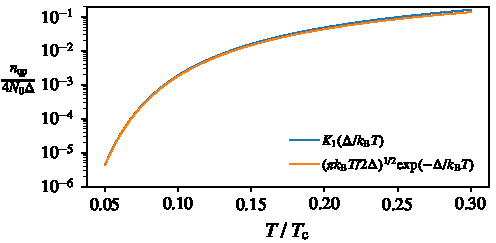
\includegraphics[width=\textwidth]{theory/reduced_thermal_qpdensity.pdf}
\caption
[The reduced thermal quasiparticle density versus reduced temperature.]
{The reduced thermal quasiparticle density versus reduced temperature, from Equation~\ref{eqn:qpdensity_thermal}.
The gap $\gap$ here is taken to be equal to its value at $\temperature = 0$, which at higher temperatures is not a good approximation.}
\label{fig:reduced_thermal_qpdensity}
\end{figure}

The quasiparticles affect the gap energy, which decreases as the quasiparticle density increases.
The BCS theory gives an implicit equation for the gap:
\begin{equation}
1
  =
  \ssdos \ucvolume \bcspotential
  \int_\gap^\infty \dd{\energy}
  \qprdos(\energy) \frac{1 - 2 \qpoccupancy(\energy)}{\energy},
\end{equation}
where the gap appears in both the lower limit of the integral and in the quasiparticle energy.
(The unit cell volume appears here because I use $\ssdos$ to mean the number of single-spin normal-metal states per unit energy \textit{per unit volume} at the Fermi energy.)
In Section~\ref{sec:theory.perturbation} I discuss a method for obtaining approximate equations for the gap.
Even in an illuminated KID, the number of excitations will generally be sufficiently small that the gap will not vary much from its value at zero temperature.


\subsection{Generation}
\label{sec:theory.quasiparticle.generation}

The quasiparticle excitations must occur in pairs, since the energy reduction is due to the pairing, so a particle that deposits energy greater than $2 \gap$ (the \textit{spectroscopic} gap) can break one or more Cooper pairs, exciting quasiparticles that eventually recombine into Cooper pairs or decay by other means.
Phonons with energy $\phononenergy > 2 \gap$ that enter the film from the substrate may also break pairs.

As we will see later, the detector sensitivity may be increased by using a high readout tone power.
Although the readout photons individually have energies much less than the gap (see Table~\ref{tab:energies}), a quasiparticle that absorbs many quanta and is excited to an energy above $3 \gap$ may scatter inelastically and create a phonon that is sufficiently energetic to break a pair.
KID experiments that use careful shielding to reduce quasiparticle generation due to stray light nevertheless observe more quasiparticles than the thermal equilibrium value, and some of this excess is typically attributed to readout generation~\autocite{deVisser2012APL,deVisser2014NatComm}.


\subsection{Pair recombination}
\label{sec:theory.quasiparticle.pair_recombination}

Quasiparticles have finite lifetimes and may decay in various ways.
For elemental BCS superconductors, the most relevant process involves two quasiparticles with energies
$\energy_1, \energy_2 \ge \gap$
recombining into a Cooper pair with the emission of a phonon with energy
$\phononenergy = \energy_1 + \energy_2 \ge 2 \gap$.
(Since a photon can break a Cooper pair and excite quasiparticles, the reverse process of recombination with photon emission is possible.
However, because the final density of states corresponding to this process is much smaller than the density of states for phonon emission, the radiative lifetime is much longer and this process is negligible~\cite{Burstein1961PRL}.)
\todo[inline]{Incorporate other refs in Rothwarf and Taylor}

\textcite{Kaplan1976PRB} derive a low-temperature equilibrium pair-recombination time, given for a quasiparticle with $\energy = \gap_\zerotemp$ by
\begin{equation}
\qprecombinationtime^{-1}
  =
  \electronphonontime^{-1}
  \pi^{1/2}
  \left( \frac{2 \gap_\zerotemp}{\kb \tc} \right)^{5/2}
  \left( \frac{\temperature}{\tc} \right)^{1/2}
  \exp \left( -\frac{\gap_\zerotemp}{\kb \temperature} \right),
\label{eqn:qprecombinationtime}
\end{equation}
where $\electronphonontime$ is the characteristic electron-phonon interaction time defined in the same reference.
The recombination rate for a given total energy is proportional to the phonon density of states at that energy, which increases with increasing energy~\autocite{Chang1978JLTP}.
Thus, quasiparticles with higher energies have shorter lifetimes.
Comparing Equation~\ref{eqn:qprecombinationtime} to Equation~\ref{eqn:qpdensity_thermal} shows that, in thermal equilibrium, the inverse recombination lifetime is proportional to the quasiparticle density:
\begin{equation}
\qprecombinationtime^{-1}
  =
  \electronphonontime^{-1}
  \left( \frac{2 \gap_\zerotemp}{\kb \tc} \right)^3
  \frac{\qpdensity}{4 \ssdos \gap_\zerotemp}.
\end{equation}
The proportionality
\begin{equation}
\qprecombination
  \equiv
  \left( \frac{2 \gap_\zerotemp}{\kb \tc} \right)^3
  \left( 4 \ssdos \gap_\zerotemp \electronphonontime \right)^{-1}
\label{eqn:qprecombination}
\end{equation}
is the quasiparticle recombination constant~\autocite{Gray1981Chapter5}.
Using values for aluminum from Table~\ref{tab:materials} gives
$\qprecombination = \SI{7.8}{\micro\meter^3.\second^{-1}}$.
The recombination constant will actually change as the gap energy varies with quasiparticle density~\autocite{Gray1971JPF, Rothwarf1974PRL}, but I will neglect this dependence.
The recombination rate per unit volume is thus quadratic in the quasiparticle density:
\begin{equation}
\rate_\qprecombination
  \equiv
  \qprecombinationtime^{-1} \qpdensity
  =
  \qprecombination \qpdensity^2.
\label{eqn:rate_qprecombination}
\end{equation}
Since recombination involves quasiparticles interacting in pairs, it is not surprising that the rate for $\qpnumber$ quasiparticles goes as $\binom{\qpnumber}{2} \propto \qpnumber^2$ to leading order~\autocite{Gray1971JPF}.

In thermal equilibrium, if quasiparticles are generated at a rate $\rate_\generation(\temperature)$ per unit volume and the only quasiparticle decay process is recombination with phonon emission, then the rate equation for the quasiparticle density is
\begin{equation}
0
  =
  \dv{\qpdensity}{\time}
  =
  \rate_{\generation}(\temperature)
  -
  \qprecombination \qpdensity(\temperature)^2.
\label{eqn:rate_qpdensity_thermal}
\end{equation}
Then, using Equation~\ref{eqn:qpdensity_thermal}, the low-temperature thermal generation rate is
\begin{equation}
\rate_{\generation}(\temperature)
  =
  \frac{4 \ssdos \gap_\zerotemp}{\electronphonontime} \left( \frac{2 \gap_\zerotemp}{\kb \tc} \right)^3 K_1(\gap_\zerotemp / \kb \temperature)^2
  \approx 
  \frac{4 \ssdos \gap_\zerotemp}{\electronphonontime} \left( \frac{2 \gap_\zerotemp}{\kb \tc} \right)^3 \frac{\pi \kb \temperature}{2 \gap_\zerotemp} \exp \left(-\frac{2 \gap_\zerotemp}{\kb \temperature}\right).
\label{eqn:rate_generation_thermal}
\end{equation}
At sufficiently low temperatures the total thermal generation rate will become negligible compared to other sources.
This reduces the effect of fluctuations in the generation rate cause by temperature fluctuations, which are common in a moving telescope.


\subsection{Phonons}
\label{sec:theory.quasiparticle.phonons}

While the various generation process act to create an occupancy that exceeds the thermal value, scattering processes act to restore the quasiparticle system to equilibrium.
\textcite{Kaplan1976PRB} derive a thermal equilibrium quasiparticle-phonon scattering time given by
\begin{equation}
\qpphononscatteringtime^{-1}
  =
  \electronphonontime^{-1} \Gamma \left(\tfrac{7}{2}\right) \zeta \left(\tfrac{7}{2}\right) \left( \frac{\kb \tc}{2 \gap_\zerotemp} \right)^{1/2} \left( \frac{\temperature}{\tc} \right)^{7/2},
\label{eqn:electron-phonon_scattering}
\end{equation}
where $\Gamma$ is the Gamma function and $\zeta$ is the Riemann zeta function.
Assuming the BCS weak-coupling relation, the numerical factors work out to
$\Gamma (7 / 2) \zeta (7 / 2) / 3.52^{1/2} \approx 1.996$.
\todo[inline]{Give scattering time with fiducial parameters.}
A quasiparticle at the gap edge cannot scatter and emit a phonon, because there no available quasiparticle states with lower energy, but at higher energies the scattering rate rapidly increases.
\todo[inline]{What about impurity scattering?}
\todo[inline]{What is the effect of electron-electron scattering? Allegedly important for aluminum. See ChangJLTP1978.}

A phonon produced by quasiparticle recombination has sufficient energy to break another Cooper pair in the same superconductor.
Such a phonon will quickly encounter the film-substrate interface, but the acoustic match between superconducting films and typical crystalline substrates tends to be poor, so phonons are likely to reflect on each encounter with the  interface~\autocite{Kaplan1979JLTP}.
These facts will significantly modify the results of the preceding section.

%In aluminum, \textcite{Kaplan1976PRB} calculate an average time $\phononpairbreakingtime = \SI{242}{ps}$ for a sufficiently energetic phonon to break a Cooper pair at low temperature, and the time decreases with increasing phonon energy.
\textcite{Chang1978JLTP} calculate a time
$\phononpairbreakingtime \sim \SI{100}{ps}$
for a sufficiently energetic phonon to break a pair, which is much less than both the inelastic scattering time and the anharmonic decay time~\autocite{Kozorezov2000PRB}.
They also calculate a phonon escape time
\begin{equation}
\phononescapetime
  =
  \frac{4 \thickness}{\efficiency \soundspeed},
\label{eqn:phononescapetime}
\end{equation}
where $\thickness$ is the film thickness, $\soundspeed$ is the speed of sound, and $\efficiency$ is the transmission probability per encounter, which may be quite small~\autocite{Kaplan1979JLTP}.
Using
$\thickness = \SI{40}{nm}$
and
$\soundspeed = \SI{6.4e3}{m.s^{-1}}$~\autocite{Chang1978JLTP}
gives
$\phononescapetime = \SI{25}{ps} / \efficiency$.

A recombination phonon must leave the film for the quasiparticle number to decrease, so the effective recombination lifetime of the quasiparticles is increased by a phonon-trapping factor~\autocite{Rothwarf1967PRL}
\begin{equation}
\phonontrapping
  =
  \left( \frac{\phononescapetime^{-1}}{\phononescapetime^{-1} + \phononpairbreakingtime^{-1}} \right)^{-1}
  =
  1 + \frac{\phononescapetime}{\phononpairbreakingtime},
\label{eqn:phonontrapping}
\end{equation}
where $\phonontrapping^{-1}$ is the probability for a phonon to escape the film instead of breaking a pair.
Depending on the composition and thickness of the film and substrate, and the details of their interface, this probability may range from just above 0 to just less than 1.
Since both the pair-breaking and escape times are much less than the quasiparticle recombination time $\qprecombinationtime$, which is usually \SIrange{1}{1000}{\micro\second} in the superconductors used for KIDs, the time spent as a phonon is negligible and nearly all of the energy resides in the quasiparticles~\autocite{Rothwarf1974PRL}.
Phonons, produced by scattering or otherwise, for which $\phononenergy < 2 \gap$ are subject to the same phonon trapping effect, but this is less important because these phonons cannot break pairs.

To capture the relevant effects of phonon trapping, we may replace the recombination constant $\qprecombination$ by an effective recombination constant
$\qprecombinationeff = \qprecombination / \phonontrapping$
in Equations~\ref{eqn:rate_qprecombination} and~\ref{eqn:rate_qpdensity_thermal}.
(Note that the thermal density of quasiparticles is independent of $\phonontrapping$: the effective quasiparticle recombination lifetime is increased by a factor $\phonontrapping$, but the thermal generation rate due to pair-breaking thermal phonons entering from the substrate is decreased by the same factor.)
Because $\phonontrapping$ is material-dependent and difficult to calculate~\autocite{Gray1981Chapter5}, the fundamental quasiparticle recombination time $\qprecombinationtime$, and thus the characteristic electron-phonon time $\electronphonontime$, are not experimentally accessible from measurements of KIDs.

\todo[inline]{Incorporate material on thickness-independent trapping}
\begin{comment}
According to Equation~\ref{eqn:phononescapetime}, the phonon trapping factor should decrease with decreasing film thickness.
\textcite{Eisenmenger1976AP}, using a ballistic phonon model and assuming specular reflection at interfaces, point out that when the film thickness $\thickness$ is much less than the mean-free path against pair-breaking, the escape time is independent of the film thickness and depends only on the critical angle for total internal reflection.
However, there seems to be no experimental evidence for this regime.
Measurements of the phonon trapping factor in aluminum films as thin as \SI{100}{nm} have shown linear dependence on film thickness [cite Long].
\end{comment}

\todo[inline]{Incorporate material on qp-phonon imbalance at short times}
%the imbalance between quasiparticles and phonons at times $\time \ll \qprecombinationtime$~\autocite{Rothwarf1967PRL}.

This model ignores the phonon population in the substrate.
The anharmonic decay time is very long in silicon~\autocite{Maris1993PRB}, so phonons that do escape from the film cannot necessarily be neglected unless they are efficiently destroyed.
\textcite{deVisser2014} shows data (in Appendix B) consistent with a large population of recombination phonons in the substrate forming the bottleneck for relaxation of the quasiparticle system.
\textcite{Patel2017PRB} show that pair-breaking phonons can propagate for several millimeters across a chip, and that they are absorbed by normal metal regions.
Phonons that escape from one detector and are absorbed in another could cause spurious response, an effect called crosstalk.


\subsection{Single-quasiparticle decay}
\label{sec:theory.quasiparticle.single_decay}

In addition to canonical recombination in pairs with phonon emission, quasiparticles may also decay through processes that decrease their number by 1.
For these processes, the total decay rate per unit volume is proportional to the quasiparticle density.

For example, magnetic flux vortices act as quasiparticle sinks~\autocite{Ullom1998APL,Wang2014NatComm}.
The gap energy is reduced inside a vortex, so a quasiparticle that diffuses into one may scatter inelastically to an energy below the gap energy outside.
It will thus remain trapped inside the vortex, and when it eventually recombines with another quasiparticle the resulting phonon energy may be less than $2 \gap$, insufficient to break a pair outside the vortex.
Quasiparticles may also become trapped in local defects~\autocite{Kozorezov2001APL} or in normal metal regions in contact with the superconductor~\autocite{Joyez1994PRL, Riwar2016PRB}.

The decay rate per unit volume due to all such single-quasiparticle sources can be written
\begin{equation}
\rate_\qpsingledecay
  =
  \sum_\alpha \qpsingledecay_\alpha \qpdensity
  \equiv
  \qpsingledecay \qpdensity,
\label{eqn:rate_qpsingledecay}
\end{equation}
where $\qpsingledecay$ is the sum of the decay constants for the individual processes.
These processes may be useful for detector engineering, but they  are not necessary to describe most of the behavior of the KIDs discussed in this work.


\subsection{Inhomogeneity and diffusion}
\label{sec:theory.quasiparticle.inhomogeneity}

While the quasiparticles are collective excitations of electrons near the Fermi surface, their typical velocities are much less than the Fermi velocity $\velocity_\fermi$.
In fact, the velocity of a quasiparticle with $\energy = \gap$ is zero.
The BCS relationship between quasiparticle group velocity $\velocity_\group$ and quasiparticle energy $\energy$ is
\begin{align}
\velocity_\group
  =
  \pdv{\energy_\momentum}{\momentum}
  =
  \frac{\blochenergyf_\momentum}{\energy_\momentum} \frac{\momentum}{\mass},
\end{align}
where $\momentum$ and $\mass$ are the electron momentum and mass.
The energy range where the quasiparticle occupancy is nonzero is a small fraction of the Fermi energy, so we take
$\momentum / \mass = \velocity_\fermi$.
Then,
\begin{equation}
\velocity_\group(\energy)
  =
  \velocity_\fermi \left( 1 - \frac{\gap^2}{\energy^2} \right)^{1/2}.
\end{equation}
As shown in Figure~\ref{fig:quasiparticle_group_velocity}, the group velocity rapidly increases with increasing quasiparticle energy to a significant fraction of the Fermi velocity.

\begin{figure}[htb]
\centering
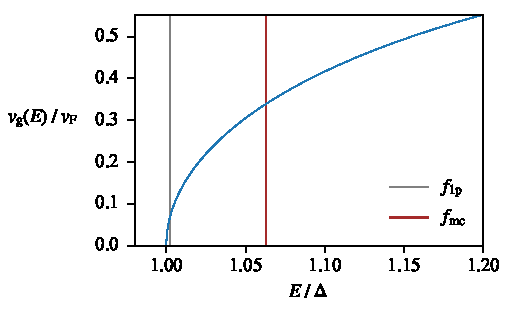
\includegraphics[width=0.9\textwidth]{theory/quasiparticle_group_velocity.pdf}
\caption[The quasiparticle group velocity versus quasiparticle energy.]
{
The quasiparticle group velocity normalized to the Fermi velocity versus quasiparticle energy normalized to the gap energy.
The blue curve is universal.
The vertical lines correspond to the energy of the gap plus one readout photon for the two fiducial readout frequencies, assuming the fiducial value for the gap energy.
We expect the first peaks in the occupancy to occur at these energies.
}
\label{fig:quasiparticle_group_velocity}
\end{figure}

The quasiparticle diffusion coefficient $\qpdiffusion$ is related to the normal-state diffusion coefficient $\normaldiffusion$ by
\begin{equation}
\qpdiffusion
  =
  \frac{\expval{\velocity_\group}}{\velocity_\fermi} \normaldiffusion,
\end{equation}
where $\expval{\velocity_\group}$ is the group velocity averaged over all quasiparticles~\autocite{Ullom1998PRB}.
The rapid variation of the group velocity with energy makes it difficult to estimate the quasiparticle diffusion coefficient without a good estimate of the nonequilibrium occupancy.
Assuming only pair recombination is relevant, a typical diffusion distance is then
$(\qpdiffusion \phonontrapping \qprecombinationtime)^{1/2}$.
This is usually long enough to reduce the problem to two dimensions.
\todo[inline]{Calculate fiducial diffusion length!}

With $\qpdensity(\time, \vb{x})$ the position-dependent density and $\nabla^2$ the Laplacian, both in two dimensions, Equation~\ref{eqn:rate_qpdensity} becomes
\begin{equation}
\pdv{\qpdensity(\time, \vb{x})}{\time}
  =
  \rate_\generation(\time, \vb{x})
  + \qpdiffusion \nabla^2 \qpdensity(\time, \vb{x})
  -\qprecombinationeff \qpdensity(\time, \vb{x})^2
  -\qpsingledecay \qpdensity(\time, \vb{x}).
\label{eqn:rate_qpdensity_diffusion}
\end{equation}
Solutions of similar equations have been attempted~\autocite{Wang2014NatComm,Nsanzineza2014PRL}.
However, when modeling detector response we will assume that the quasiparticle density is homogeneous in some volume $\volume$.
This will allow us to switch freely between quasiparticle density $\qpdensity$ and number $\qpnumber = \volume \qpdensity$.
The readout signal will tend to produce peaks in the occupancy at energies that are greater than the gap by integer multiples of the readout photon energy.
Thus, we expect more rapid diffusion than the thermal average quasiparticle velocity would suggest.
Additionally, since the local recombination time increases rapidly with decreasing density, those quasiparticles that diffuse away from a high-density region may travel much farther than the typical diffusion length in higher-density regions.
In hybrid KIDs, in which quasiparticles are trapped in a high-current region, diffusion tends to equalize the density.
In single-metal KIDs, such as the all-aluminum lumped-element devices discussed here, quasiparticles that diffuse into low-current regions of the capacitors are effectively lost.

\section{Electrodynamics}
\label{sec:theory.electrodynamics}

\subsection{The two-fluid model}
\label{sec:theory.electrodynamics.two-fluid}

\todo[inline]{Give and discuss London equations, and limitations.}
%Long before the BCS theory was developed, the electrodynamic response of a superconductor was described by the phenomenological London theory.

A simple model that gives qualitatively correct results for the electrodynamics of a superconductor involves treating the Cooper pair condensate and the quasiparticle excitations as two fluids with different behavior.
Using a Drude model, the quasiparticles are treated as normal electrons with a scattering time $\tau_\normal$, while the condensate is treated by taking its scattering time to be infinite.
This requires extending Ohm's law
$\vb{\currentdensity} = \conductivity \vefield$
to a complex conductivity
$\conductivity = \reconductivity - \I \imconductivity$.
For angular frequencies $\omega$ such that
$\omega \tau_\normal \ll 1$
and
$\hbar \omega < 2 \gap$,
this leads to~\autocite{Tinkham2004}
\begin{align}
\reconductivity(\omega)
  &=
  \frac{\pi n_\superconducting \unitcharge^2}{2 \mass} \delta(\omega)
  + \frac{n_\normal \unitcharge^2 \tau_\normal}{\mass}; \\
\imconductivity(\omega)
  &=
  \frac{n_\superconducting \unitcharge^2}{\mass \omega},
\label{eqn:two-fluid_conductivity}
\end{align}
where $n_\mathrm{n, s}$ are respectively the densities of the normal and superconducting fluids, and $\delta$ is the delta function.
This model predicts perfect conductivity only at zero frequencies, and some dissipation at nonzero frequencies whenever  excitations are present.
It also predicts a large kinetic inductance, an effect which is negligible in normal metals: a significant amount of energy from the field is converted into the kinetic energy of the superconducting fluid (that is, the Cooper pairs) and is then released when the field changes direction.
This effect causes the supercurrent to lag the electric field.
While these conclusions are useful, to describe KID response we need a more sophisticated model based on the BCS theory.


\subsection{The Mattis-Bardeen theory}
\label{sec:theory.electrodynamics.mattis-bardeen}

\todo[inline]{Give Chambers expression and discuss cutoffs in the spatial integral.}
\textcite{MattisBardeen1958PR} derived expressions for the relationship between the current density and vector potential for normal metals and, starting from the BCS theory, for superconducting metals.
Their most general expression involves a spatial integral because the response is non-local.
However, in the extreme anomalous limit, where the penetration depth $\penetrationdepth$ is much less than the coherence length $\coherencelength$, they derive equations that are effectively local.
These expressions should also be valid for the aluminum films discussed in this thesis, which are sufficiently thin that scattering at the film interfaces limits the mean free path $\meanfreepath$ to a length of order $\thickness$, the film thickness.
The ratios of the real and imaginary parts of the complex conductivity to the normal state conductivity $\normalconductivity$ are
\begin{align}
\begin{split}
\frac{\reconductivity}{\normalconductivity}
  &=
  \frac{2}{\planck \freadout} \int_\gap^\infty \dd{\energy}
  \left[ \qpoccupancy(\energy) - \qpoccupancy(\energy + \planck \freadout) \right]
  \frac{\energy^2 + \gap^2 + \planck \freadout \energy}
  {[\energy^2 - \gap^2]^{1/2} [(\energy + \planck \freadout)^2 - \gap^2]^{1/2}} \\
  &\quad +
  \frac{1}{\planck \freadout} \int_{\gap - \planck \freadout}^{-\gap} \dd{\energy}
  \left[ 1 - 2 \qpoccupancy(\energy + \planck \freadout) \right]
  \frac{\energy^2 + \gap^2 + \planck \freadout \energy}
  {[\energy^2 - \gap^2]^{1/2} [(\energy + \planck \freadout)^2 - \gap^2]^{1/2}};
\end{split}
\label{eqn:mattisbardeen1}
\end{align}
and
\begin{equation}
\frac{\imconductivity}{\normalconductivity}
  =
  \frac{1}{\planck \freadout} \int_{\gap - \planck \freadout; -\gap}^{\gap} \dd{\energy}
  \left[ 1 - 2 \qpoccupancy(\energy + \planck \freadout) \right]
  \frac{\energy^2 + \gap^2 + \planck \freadout \energy}
  {[\gap^2 - \energy^2]^{1/2} [(\energy + \planck \freadout)^2 - \gap^2]^{1/2}}.
\label{eqn:mattisbardeen2}
\end{equation}
For $\planck \freadout < 2 \gap$, the second integral in Equation~\ref{eqn:mattisbardeen1} is not present and the lower limit of the integral in Equation~\ref{eqn:mattisbardeen2} is $\gap - \planck \freadout > -\gap$, while for $\planck \freadout > 2 \gap$ the lower limit of this integral is $-\gap$.
At temperature
$\temperature = 0$
no quasiparticles are excited, so $\qpoccupancy = 0$ and $\reconductivity(\temperature = 0) = 0$;
as derived in Appendix~\ref{chp:first-order_response},
$\imconductivity(\temperature = 0) = \pi \gap_\zerotemp \normalconductivity / \planck \freadout$.
The zero-temperature frequency dependence is the same as in the two-fluid model, but this is not true at nonzero temperatures.


\subsection{Surface impedance}
\label{sec:theory.electrodynamics.surface_impedance}

The complex conductivity describes the local response of the current density to an applied field.
However, the relationship between the fields at the metal surface and the complex conductivity has additional dependence on geometry.
These effects can be described using the surface impedance $\impedance_\surface = \resistance_\surface + \I \reactance_\surface$,
where
$\resistance_\surface$ is the surface resistance and $\reactance_\surface$ is the surface reactance.
The relationship between the surface reactance and the kinetic inductance is $\reactance_\surface = 2 \pi \freadout \inductance_\kinetic$.
If $\penetrationdepth$ is the effective penetration depth at $\temperature = 0$, then the surface impedance is purely reactive:
\begin{equation}
\impedance_\surface(0)
  =
  \I \reactance_\surface(0)
  =
  2 \pi \I \impedance_\vacuum \freadout \penetrationdepth / \lsvac.
\end{equation}
The effective penetration depth, which depends on the geometry, is much less than the free space wavelength, so the surface reactance is much less than the vacuum impedance.

Changes in the complex conductivity alter the surface impedance. In some simple cases this relationship can be written~\autocite{Zmuidzinas2012ARCMP}
\begin{equation}
\impedance_\surface
  =
  \impedance_\surface(0) \left(\frac{\conductivity}{\conductivity(0)}\right)^{-\surfimpexp}
  =
  \impedance_\surface(0)
  \left( 1 + \I \frac{\conductivity - \conductivity(0)}{\imconductivity(0)} \right)^{-\surfimpexp}.
\label{eqn:surface_impedance.response}
\end{equation}
Under the conditions discussed in this work, both the real and imaginary parts of $[\conductivity - \conductivity(0)] / \imconductivity(0)$ will turn out to be small, so we can use a first-order approximation for the relationship between a shift in the conductivity and a shift in the surface impedance:
\begin{equation}
\impedance_\surface
  \approx
  \impedance_\surface(0) \left( 1 - \surfimpexp \frac{\conductivity - \conductivity(0)}{\conductivity(0)} \right)
  =
  \impedance_\surface(0) \left( 1 - \I \surfimpexp \frac{\conductivity - \conductivity(0)}{\imconductivity(0)} \right).
\end{equation}
The shift from the zero-temperature surface impedance is thus
\begin{equation}
\impedance_\surface - \impedance_\surface(0)
  =
  \resistance_\surface + \I [\reactance_\surface - \reactance_\surface(0)]
  =
  \surfimpexp \reactance_\surface(0)
  \left( \frac{\reconductivity - \I [\imconductivity - \imconductivity(0)]}{\imconductivity(0)} \right).
\label{eqn:impedance_surface_first_order}
\end{equation}
We see that the first-order approximation allows us to separate real and imaginary components cleanly:
\begin{align}
\begin{split}
\resistance_\surface
  &=
  \surfimpexp \reactance_\surface(0) \frac{\reconductivity}{\imconductivity(0)}; \\
\reactance_\surface - \reactance_\surface(0)
  &=
  -\surfimpexp \reactance_\surface(0) \frac{\imconductivity - \imconductivity(0)}{\imconductivity(0)}.
\end{split}
\label{eqn:surface_resistance_and_reactance_shift}
\end{align}
These equations are used later to calculate detector responsivity.

In the thin film, local limit discussed above, where the electron mean free path is limited by diffusive scattering at the surfaces,
$\surfimpexp = 1$; also in this limit, the zero-temperature surface impedance is
$\impedance_\surface(0) = \I / \imconductivity(0) \thickness$,
where $\thickness$ is the film thickness~\autocite{Zmuidzinas2012ARCMP}.
\todo[inline]{Mention that Zs goes as 1 / d2 here.}
This leads to a simple relationship between the surface impedance and complex conductivity:
\begin{equation}
\impedance_\surface
  =
  \frac{1}{\thickness \conductivity}
  \approx
  \frac{\reconductivity}{\thickness \imconductivity^2}
  + \frac{\I}{\thickness \imconductivity},
\end{equation}
using $\reconductivity / \imconductivity \ll 1$, which is true at low temperatures.
\todo[inline]{Understand and explain various limits relevant for surface impedance: extreme anomalous, thick film, thin film, etc.}



\section{Nonequilibrium perturbations to the ground state}
\label{sec:theory.perturbation}

\subsection{Nonequilibrium occupancy}
\label{sec:theory.perturbation.nonequilibrium}

Ideally, the temperature of a KID will be sufficiently low that the optical illumination will create quasiparticle excitations far in excess of thermal values.
The strong readout signal will also tend to shift the occupancy to higher energies and may also break pairs.
Thus, an operating KID may be far from thermal equilibrium, and there is strong evidence that nonequilibrium effects must be considered to understand even the qualitative behavior of KIDs in some regimes~\autocite{deVisser2014PRL,Budoyo2016PRB}.

The Mattis-Bardeen equations (\ref{eqn:mattisbardeen1} and \ref{eqn:mattisbardeen2}) allow us to calculate the complex conductivity with knowledge of the quasiparticle occupancy.
However, for a film out of equilibrium, the occupancy is not directly specified by the experimental conditions.
Instead, the independent quantities are the rates at which optical photons, readout photons, and phonons from the substrate are incident on the resonator.
The equations for the shift in the gap energy, the quasiparticle density, and the complex conductivity all involve the quasiparticle occupancy, and must be determined self-consistently.
This problem is difficult to solve analytically.
Numerical solutions of kinetic equations for the coupled non-equilibrium quasiparticle and phonon occupancies~\autocite{Chang1977PRB, Chang1978JLTP}
have been produced by at least two groups~\autocite{Goldie2013SUST, Budoyo2016PRB}, but such code has not been made publicly available.
One important result of the simulations is that the occupancy develops large peaks at energies that exceed the gap by integer multiples of the readout photon energy, as quasiparticles absorb readout photons.
\todo[inline]{Discuss Cambridge papers on occupancies, Budoyo, and SRON papers.}


\subsection{First-order response functions}
\label{sec:theory.perturbation.first-order}

To handle nonequilibrium effects perturbatively, I follow \textcite{Zmuidzinas2012ARCMP} and obtain expressions for the response of the superconducting film that are correct to first order in $\qpoccupancy$, which is taken to be determined by the experimental conditions.
If $C(0)$ is the value at $\temperature = 0$ (where no quasiparticles are excited) of some quantity that depends on the quasiparticle occupancy, then the first-order response function $\responseqpoccupancy_C(\energy)$ is given by
\begin{equation}
C - C(0)
  \approx
  \int_0^\infty \dd{\energy} \responseqpoccupancy_C(\energy) \qpoccupancy(\energy)
  =
  \braket{\responseqpoccupancy_C}{\qpoccupancy},
\end{equation}
using Dirac inner product notation.
(The response functions will turn out to be proportional to the superconducting density of states.)
Note that these first-order expressions describe the shifts from the zero-temperature values: $\qpdensity$, $\reconductivity$, and $\resistance_\surface$ vanish at $\temperature = 0$, while $\gap$, $\imconductivity$, and $\reactance_\surface$ do not.
In this section I give the response functions for the gap, the quasiparticle number, and the conductivity of the film, and evaluate the integrals for a thermal occupancy.
See Appendix~\ref{chp:first-order_response} for the derivations.

\todo[inline]{Plot $\gap(\temperature)$ from first-order shift and compare to exact BCS expression.}
\begin{comment}
\begin{figure}[htb]
\centering
\missingfigure[figwidth=\textwidth]{Plot $\gap(\temperature)$ from first-order shift and compare to exact BCS expression.}
\caption[Approximate and exact expressions for the gap energy versus temperature.]
{Approximate and exact expressions for the gap energy versus temperature.}
\label{fig:gap_versus_temperature}
\end{figure}
\end{comment}

\todo[inline]{Give exact BCS expression for the gap.}
The response function for the gap is
\begin{equation}
\responseqpoccupancy_\gap
  =
  - \frac{2 \gap_\zerotemp}{\left(\energy^2 - \gap_\zerotemp^2\right)^{1/2}}
  =
  - \frac{2 \gap_\zerotemp \qprdos_\zerotemp(\energy)}{\energy},
\end{equation}
where $\gap_\zerotemp$ is the value of the gap at $\temperature = 0$ and $\qprdos_\zerotemp$ is the reduced density of states using this gap value.
This response function is negative because quasiparticles reduce the gap.
The reduction effect rapidly decreases with increasing quasiparticle energy.

From Equation~\ref{eqn:qpdensity}, we can read off the response function for the quasiparticle density:
\begin{equation}
\responseqpoccupancy_{\qpdensity}
  =
  4 \ssdos \Re{\frac{\energy}{\left(\energy^2 - \gap_\zerotemp^2\right)^{1/2}}}
  \equiv
  4 \ssdos \qprdos_\zerotemp(\energy).
\end{equation}
The zero-temperature gap $\gap_\zerotemp$ appears here because the shift in the gap produces a second-order effect.

The response function for the real part of the conductivity is
\begin{equation}
\responseqpoccupancy_{\reconductivity}(\energy)
  =
  \frac{2 \normalconductivity \qprdos_\zerotemp(\energy)}{\planck \freadout}
  \left[
  \qprdos_\zerotemp(\energy + \planck \freadout)
  \left(1 + \frac{\gap_\zerotemp^2}{\energy (\energy + \planck \freadout)} \right)
  - \qprdos_\zerotemp(\energy - \planck \freadout)
  \left(1 + \frac{\gap_\zerotemp^2}{(\energy - \planck \freadout) \energy} \right)
  \right].
\label{eqn:responseqpoccupancy_reconductivity}
\end{equation}
For a thermal occupancy,
\begin{equation}
\frac{\braket{\responseqpoccupancy_{\reconductivity}}{\qpoccupancy(\temperature)}}{\normalconductivity}
  =
  \frac{4 \gap_\zerotemp}{\planck \freadout}
  \exp \left( -\frac{\gap_\zerotemp}{\kb \temperature} \right)
  \sinh \left( \frac{\planck \freadout}{2 \kb \temperature} \right)
  K_0 \left( \frac{\planck \freadout}{2 \kb \temperature} \right),
\label{eqn:responseqpoccupancy_reconductivity_thermal}
\end{equation}
where $K_0$ is the zero-order modified Bessel function of the second kind, not to be confused with a response function.

The response function for the imaginary part of the conductivity is
\begin{equation}
\responseqpoccupancy_{\imconductivity}(\energy)
  =
  - \frac{2 \normalconductivity \qprdos_\zerotemp(\energy)}{\planck \freadout}
  \left[
  \frac{\pi \gap_\zerotemp}{\energy}
  +   \left( 1 + \frac{\gap_\zerotemp^2}{\energy (\energy - \planck \freadout)} \right)
  \frac{\stepfunction(\gap_\zerotemp + \planck \freadout - \energy) (\energy - \planck \freadout)}{[\gap_\zerotemp^2 - (\energy - \planck \freadout)^2]^{1/2}}
  \right],
\label{eqn:responseqpoccupancy_imconductivity}
\end{equation}
where $\stepfunction$ is the unit step function.
For a thermal occupancy,
\begin{equation}
\frac{\braket{\responseqpoccupancy_{\imconductivity}}{\qpoccupancy(\temperature)}}{\normalconductivity}
  =
  -\frac{2 \pi \gap_\zerotemp}{\planck \freadout}
  \left[
  K_0 \left( \frac{\gap_\zerotemp}{\kb \temperature} \right)
  + \exp \left( -\frac{\gap_\zerotemp}{\kb \temperature} \right)
  \exp \left( -\frac{\planck \freadout}{2 \kb \temperature} \right)
  I_0 \left( \frac{\planck \freadout}{2 \kb \temperature} \right)
  \right],
\label{eqn:responseqpoccupancy_imconductivity_thermal}
\end{equation}
where $I_0$ is the zero-order modified Bessel function of the first kind.

\begin{figure}[htb]
\centering
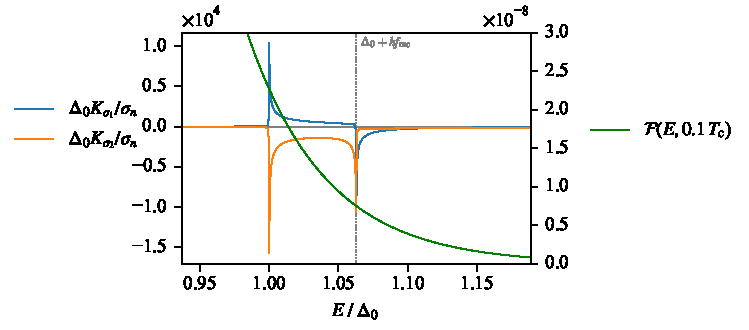
\includegraphics[width=\textwidth]{theory/responseqpoccupancy_conductivity_f_mc.pdf}
\caption
[The first-order response functions for the real and imaginary parts of the conductivity at $\freadout_\multichroic$.]
{The first-order response functions for the real and imaginary parts of the conductivity at $\freadout_\multichroic = \SI{3.0}{GHz}$ versus energy in units of the gap, and a thermal occupancy.
The left axis shows Equations~\ref{eqn:responseqpoccupancy_reconductivity} and~\ref{eqn:responseqpoccupancy_imconductivity} multiplied by constants to make them dimensionless.
For display, the density of states factors have been broadened using $\mitrovic / \gap_\zerotemp = 0.0002$.
The right axis shows a thermal occupancy at a typical KID operating temperature.
Figure~\ref{fig:responseqpoccupancy_conductivity_f_1p} shows the same quantities at a much lower frequency, where the peaks in the response functions are closer together.}
\label{fig:responseqpoccupancy_conductivity_f_mc}
\end{figure}

These expressions for $\responseqpoccupancy_{\reconductivity}$ and $\responseqpoccupancy_{\imconductivity}$ are plotted for two different frequencies in Figures~\ref{fig:responseqpoccupancy_conductivity_f_mc} and~\ref{fig:responseqpoccupancy_conductivity_f_1p}.
The absorption of readout photons by the quasiparticle system may decrease the occupancy at the gap and increase it at integer multiples of the readout photon energy.
While $\responseqpoccupancy_{\imconductivity}$ is negative for quasiparticles at all energies, $\responseqpoccupancy_{\reconductivity}$ is positive for frequencies near the gap but is negative for quasiparticles with energies higher than the gap plus one readout photon.
Shifting a quasiparticle from $\gap_\zerotemp$ to $\gap_\zerotemp + \planck \freadout$ will have a minor effect on $\imconductivity$, but will flip the sign of its effect on $\reconductivity$.
Thus, we expect the readout signal to have a larger effect on the dissipation in a resonator than on its resonance frequency.

To discuss perturbations around a steady-state situation in Section~\ref{sec:theory.response}, I use these response functions with the additional \textit{proportional-perturbation} assumption, namely, that perturbations $\delta\qpoccupancy$ to the occupancy are proportional to the steady-state occupancy $\ssqpoccupancy$.
If the perturbation varies in time, then $\delta\qpoccupancy(\energy, \time) / \ssqpoccupancy(\energy) = \epsilon(\time)$ for all energies $\energy$, where $\epsilon(\time) \ll 1$ (usually) is the fractional size of the perturbation.
This assumption is not necessarily true, especially for larger perturbations, but it greatly simplifies calculations because, as discussed in Section~\ref{sec:theory.qpnumber}, it allows us to write all perturbations in terms of perturbations to the quasiparticle number.

If
$C - C(0) = \braket{\responseqpoccupancy_C}{\qpoccupancy}$
is the shift in some quantity $C$ from the zero-temperature value $C(0)$ resulting from the occupancy $\ssqpoccupancy$,
and if
$\delta C(\time) = \braket{\responseqpoccupancy_C}{\delta\qpoccupancy(\time)}$
is the perturbation to the steady-state value resulting from a perturbation $\delta\qpoccupancy(\time)$ to $\ssqpoccupancy$,
we have
\begin{equation}
\epsilon(\time)
  =
  \frac{\delta\qpoccupancy(\energy, \time)}{\ssqpoccupancy(\energy)}
  =
  \frac{\braket{\responseqpoccupancy_C}{\delta\qpoccupancy(\time)}}
  {\braket{\responseqpoccupancy_C}{\ssqpoccupancy}}
  =
  \frac{\delta C(\time)}{C - C(0)}.
\end{equation}
That is, the fractional perturbations to all such quantities are equal.
Equivalently, the derivative of one first-order quantity with respect to another equals the ratio of the shifts from the zero temperature values:
\begin{equation}
\frac{\delta A(\time)}{\delta B(\time)}
  =
  \frac{\braket{\responseqpoccupancy_A}{\delta\qpoccupancy(\time)}}
  {\braket{\responseqpoccupancy_B}{\delta\qpoccupancy(\time)}}
  =
  \frac{\braket{\responseqpoccupancy_A}{\qpoccupancy}}
  {\braket{\responseqpoccupancy_B}{\qpoccupancy}}
  =
  \frac{A - A(0)}{B - B(0)},
\end{equation}
which is constant in time.

\section{The quasiparticle number model}
\label{sec:theory.qpnumber}

In this section I discuss the steady-state and dynamical behavior of the quasiparticle system using only the density of quasiparticles
$\qpdensity = \braket{\responseqpoccupancy_{\qpdensity}}{\qpoccupancy}$ instead of the function $\qpoccupancy(\energy)$.
The key results are the rate equation for the quasiparticle density (Equation~\ref{eqn:rate_qpdensity}) and its solutions in steady-state (Equation~\ref{eqn:ssqpdensity}) and for time-dependent perturbations (Equation~\ref{eqn:delta_qpdensity_time}).
A new phenomenological quantity emerges: the quasiparticle relaxation time $\qprelaxationtime$, which describes the decay of small perturbations to the density.

\begin{figure}[htb]
\centering
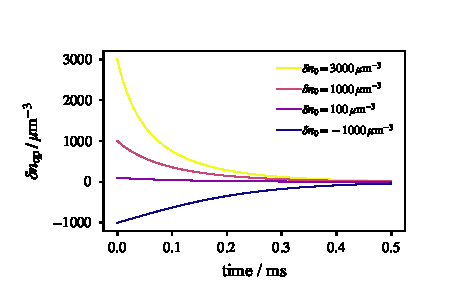
\includegraphics[width=\textwidth]{theory/delta_qpdensity_versus_time.pdf}
\caption
[The decay of perturbations to the quasiparticle density versus time.]
{The decay of perturbations to the quasiparticle density versus time.
The steady-state density is
$\ssqpdensity = \SI{1000}{\micro\meter^{-3}}$,
the effective recombination constant is
$\qprecombinationeff = \SI{3.9}{\micro\meter^{3}.s^{-1}}$
using fiducial values for aluminum with a phonon trapping factor
$\phonontrapping = 2$,
and the single-quasiparticle decay constant $\qpsingledecay$ is zero.
The resulting quasiparticle relaxation time is
$\qprelaxationtime = \SI{127}{\micro\second}$.
Large positive perturbations to the steady-state density can be caused by high-energy photons or other energetic particles.
Large negative perturbations are not expected to occur normally, but they could be created by an abrupt increase in a constant level of illumination.
There is a significant difference in behavior of the two solutions with initial conditions of opposite sign.
Because the sign of the quadratic term in Equation~\ref{eqn:rate_delta_qpdensity} is always negative, large negative perturbations initially relax more slowly to the steady-state value than large positive perturbations, and this distinction vanishes when the perturbation is small.
\todo[inline]{Recreate this $\qpdensity(\time)$ figure with a smaller steady-state density.}
}
\label{fig:delta_qpdensity_versus_time}
\end{figure}

Using Equation~\ref{eqn:rate_qprecombination} (with phonon trapping included) and Equation~\ref{eqn:rate_qpsingledecay}, the rate equation for the evolution of a homogeneous quasiparticle density is
\begin{equation}
\dv{\qpdensity(\time)}{\time}
  =
  \rate_\generation(\time)
  - \rate_\qprecombinationeff(\time)
  - \rate_\qpsingledecay(\time)
  =
  \rate_\generation(\time)
  -\qprecombinationeff \qpdensity(\time)^2
  -\qpsingledecay \qpdensity(\time).
\label{eqn:rate_qpdensity}
\end{equation}
The first term is the total generation rate per unit volume.
The second and third terms are, respectively, the decay rates per unit volume due to quasiparticle recombination in pairs with phonon emission (including phonon trapping) and due to single-quasiparticle decay.
See Appendix~\ref{chp:connections} for discussion of similar rate equations.


\subsection{Steady-state}
\label{sec:theory.qpnumber.steady-state}

For a constant generation rate
$\rate_\generation(\time) = \ssrate_\generation$,
the time derivative is zero and solving the quadratic equation
\begin{equation}
0
  =
  \ssrate_\generation
  - \qprecombinationeff \ssqpdensity^2
  - \qpsingledecay \ssqpdensity
\label{eqn:ssrate_qpdensity}
\end{equation}
gives the steady-state quasiparticle density
\begin{equation}
\ssqpdensity
  =
  \left[ \left(\frac{\qpsingledecay}{2 \qprecombinationeff}\right)^2
  + \frac{\ssrate_\generation}{\qprecombinationeff} \right]^{1/2}
  - \frac{\qpsingledecay}{2 \qprecombinationeff}.
\label{eqn:ssqpdensity}
\end{equation}
When single-quasiparticle decay is negligible, as we expect to be the case in an illuminated KID, the steady-state density is simply
$
\ssqpdensity
  =
  \left( \ssrate_\generation / \qprecombinationeff \right)^{1/2}.
$
This square-root behavior causes the detector response to be inherently nonlinear for large signals.

\subsection{Dynamics}
\label{sec:theory.qpnumber.dynamics}

To understand the behavior of perturbations around the steady-state density, it is convenient to rewrite Equation~\ref{eqn:rate_qpdensity} in terms of 
$\delta \qpdensity(\time) = \qpdensity(\time) - \ssqpdensity$
and
$\delta\rate_\generation(\time) = \rate_\generation(\time) - \ssrate_\generation$.
Using Equation~\ref{eqn:ssrate_qpdensity} to cancel most of the steady-state values gives
\begin{align}
\begin{split}
\dv{\qpdensity(\time)}{\time}
  =
  \dv{\delta\qpdensity(\time)}{\time}
  &=
  \ssrate_\generation + \delta\rate_\generation(\time)
  -
  \qprecombinationeff \left(\ssqpdensity^2 + 2 \ssqpdensity \delta\qpdensity(\time) + \delta\qpdensity(\time)^2 \right)
  - \qpsingledecay \left( \ssqpdensity + \delta\qpdensity(\time) \right) \\
  &=
  \delta \rate_\generation(\time)
  - \qprecombinationeff \delta\qpdensity(\time)^2
  - \left(2 \qprecombinationeff \ssqpdensity + \qpsingledecay \right) \delta\qpdensity(\time), \\
  &\equiv
  \delta \rate_\generation(\time)
  - \qprecombinationeff \delta\qpdensity(\time)^2
  - \qprelaxationtime^{-1} \delta\qpdensity(\time).
\end{split}
\label{eqn:rate_delta_qpdensity}
\end{align}
Here, $\qprelaxationtime$ is the quasiparticle relaxation time, which can be expressed in several useful forms using Equation~\ref{eqn:ssqpdensity}:
\begin{equation}
\qprelaxationtime
  =
  \left( 2 \qprecombinationeff \ssqpdensity + \qpsingledecay \right)^{-1}
  =
  \left( \frac{2 \ssrate_\generation}{\ssqpdensity} - \qpsingledecay \right)^{-1}
  =
  \left( 4 \qprecombinationeff \ssrate_\generation + \qpsingledecay^2 \right)^{-1/2}
  =
  \pdv{\ssqpdensity}{\ssrate_\generation}.
\label{eqn:qprelaxationtime}
\end{equation}
The relaxation time is important both as a probe of the microscopic physics and as a detector parameter to be optimized.
Before discussing it at length, I examine the behavior of solutions to Equation~\ref{eqn:rate_delta_qpdensity} in two different limits that are relevant to detector operation.

First, consider small perturbations $\delta\rate_\generation$ to the generation rate that maintain the density close to the steady-state value.
The quadratic term will be much smaller than the linear term when a perturbation $\delta\qpdensity$ is sufficiently small to satisfy
\begin{equation}
1
  \gg
  \qprecombinationeff \qprelaxationtime |\delta\qpdensity|
  =
  \frac{|\delta\qpdensity|}{2 \ssqpdensity + \qpsingledecay / \qprecombinationeff}.
\end{equation}
Thus, perturbations that are significantly smaller than the steady-state density are always small, and larger perturbations may also be small if single-quasiparticle decay is significant.
Assume that the generation rate may vary around the mean value but that we can neglect the quadratic term.
Since the optical generation rate is proportional to the absorbed power, this situation corresponds to a KID detecting a small, time-varying signal, as in CMB observation.
Defining Fourier transforms of the time-dependent quantities
\begin{equation}
\delta\qpdensity(\time)
  =
  \int_{-\infty}^\infty \dd{\faudio}
  \exp(2 \pi \I \faudio \time) \, \delta\qpdensity(\faudio)
  \qqtext{and}
\delta\rate_\generation(\time)
  =
  \int_{-\infty}^\infty \dd{\faudio}
  \exp(2 \pi \I \faudio \time) \, \delta\rate_\generation(\faudio),
\end{equation}
a Fourier solution to the linearized form of Equation~\ref{eqn:rate_delta_qpdensity} is
\begin{equation}
\delta\qpdensity(\faudio)
  =
  \frac{\qprelaxationtime}{1 + 2 \pi \I \faudio \qprelaxationtime} \delta\rate_\generation(\faudio).
\label{eqn:delta_qpdensity_frequency}
\end{equation}
As expected, the low-frequency limit of this equation equals the derivative of the steady-state density:
\begin{equation}
\lim_{\faudio \rightarrow 0} \frac{\delta\qpdensity(\faudio)}{\delta\rate_\generation(\faudio)}
  =
  \qprelaxationtime
  =
  \pdv{\ssqpdensity}{\ssrate_\generation}.
\end{equation}
The response to small, time-varying signals has single-pole behavior with a cutoff frequency 
$\faudio_\quasiparticle = (2 \pi \qprelaxationtime)^{-1}$.
This indicates that the spectral density of the quasiparticle density (or number) fluctuations has a Lorentzian shape with a bandwidth set by the relaxation time.
\todo[inline]{and this conclusion is derived more rigorously in Appendix~chp:fluctuations}

Second, consider a sudden perturbation $\delta\qpdensity(0)$ that is sufficiently large that we can neglect fluctuations in the generation rate and set
$\delta\rate_\generation = 0$.
This is a reasonable description of a KID that absorbs a high-energy photon or is hit by a cosmic ray, both of which may quickly generate a large number of quasiparticles.
(There is no physical process that is expected to instantly annihilate a large number of quasiparticles.
However, immediately after an abrupt increase in an otherwise constant illumination rate the initial perturbation would be negative, though it must satisfy
$\delta\qpdensity(0) > -\ssqpdensity$.)
In this limit, the solution for $\time > 0$ is 
\begin{equation}
\delta\qpdensity(\time)
  =
  \frac{\delta\qpdensity(0)}
  {1 + [1 + \qprecombinationeff \qprelaxationtime \delta\qpdensity(0)] 
  [\exp(\time / \qprelaxationtime) - 1]}.
\label{eqn:delta_qpdensity_time}
\end{equation}
\todo[inline]{In Appendix ... I derive this solution and discuss some of its implications for the measurement of high-energy photons.}
Even for large perturbations where $\qprecombinationeff \qprelaxationtime \, \delta\qpdensity(0) \gg 1$, after a time of order $\qprelaxationtime$ the system will have recovered to an excess density $\delta\qpdensity \sim (\qprecombinationeff \qprelaxationtime)^{-1} = 2 \ssqpdensity + \qpsingledecay / \qprecombinationeff$.
When a perturbation satisfies
$\qprecombinationeff \qprelaxationtime |\delta\qpdensity(\time)| \ll 1$,
either initially or after some decay, the behavior of the solution at later times is exponential decay to the steady-state value, which is also the solution of the rate equation when the quadratic term is negligible.
This extremely rapid decay from large density perturbations is a major advantage for CMB observation, since such perturbations are likely to render the data useless until the density approaches the steady-state value.

Figure~\ref{fig:mkidarray02_chosen_one_x_fold_fit} shows a fit of Equation~\ref{eqn:delta_qpdensity_time} to time-ordered data from one of the co-planar waveguide KIDs described in Chapter~\ref{chp:multichroic}.
The detector was illuminated by light from an electronic millimeter-wave source described in Section~\ref{sec:sensitivity.measuring} and Appendix~\ref{sec:hardware.mmw_source}.
The data shows the response as the illumination is turned off.
(More of this data set is shown in Figure~\ref{fig:mkidarray02_chosen_one_mmw_decimated_and_folded}.)
The quasiparticle relaxation time given in the legend is extracted from the fit.
It should be possible to measure $\qprecombinationeff$ by combining careful measurements of detector response to thermal quasiparticles with measurements at different illumination levels.

\begin{figure}[htb]
\centering
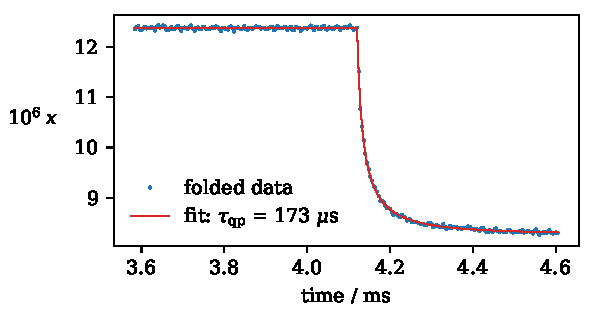
\includegraphics[width=\textwidth]{theory/mkidarray02_chosen_one_x_fold_fit.pdf}
\caption[Time-ordered data showing the detuning response as a millimeter-wave signal is turned off, and a fit.]
{
Time-ordered data showing the detuning response as a millimeter-wave signal is turned off, and a fit to Equation~\ref{eqn:rate_delta_qpdensity} multiplied by a constant.
The quantity plotted on the vertical axis is the response of the detector expressed as a fractional shift in the resonance frequency, discussed in Section~\ref{sec:theory.resonator} below.
}
\label{fig:mkidarray02_chosen_one_x_fold_fit}
\end{figure}


\subsection{The quasiparticle relaxation time}
\label{sec:theory.qpnumber.qprelaxationtime}

From the expression
$\qprelaxationtime
  =
  \left( 4 \qprecombinationeff \ssrate_\generation + \qpsingledecay^2 \right)^{-1/2}$,
we see that the relaxation time depends on all the microscopic creation and annihilation processes:
$\ssrate_\generation$ is the sum of generation rates from all sources,
$\qprecombinationeff = \qprecombination / \phonontrapping$
involves pair recombination modified by phonon trapping, and $\qpsingledecay$ includes all single-quasiparticle decay sources.
The two solutions to the rate equation discussed above illustrate the two common methods for measuring $\qprelaxationtime$ directly.
One method, shown in Figure~\ref{fig:mkidarray02_chosen_one_x_fold_fit}, involves fitting the decay back to steady-state in order to extract the time constant governing the exponential tail of the decay.
Another method involves fitting the roll-off in the spectral density of time-ordered data, which requires the quasiparticle noise to be measurable.
Both of these methods require the quasiparticle bandwidth $\faudio_\quasiparticle$ to be much less than either the bandwidth of the resonator or the bandwidth of the readout system.

The exponential temperature dependence of the thermal generation rate makes it possible to reduce it to very low levels.
At sufficiently low temperatures, some other generation source may dominate, such as readout photons or optical photons leaking into a nominally sealed package.
When the total generation rate becomes constant as the temperature is further reduced, $\qprelaxationtime$ will saturate, or remain constant at some maximum value~\autocite{deVisser2011PRL}.
Alternatively, if some single-quasiparticle decay channel becomes dominant at sufficiently low density, $\qprelaxationtime$ will saturate because the decay rate per quasiparticle is independent of the density.
Merely observing saturation does not allow us to identify its cause.

\todo[inline]{Decide how much of this to include.}
\begin{comment}
In this section I give a quick survey of experimental results regarding quasiparticle behavior at low densities and connect these results to the experimental situation in our laboratory.
The conclusion will be that single-quasiparticle decay is not necessary to explain saturation of the relaxation time in our experiments, and that the relaxation time is instead likely to be limited by optical quasiparticle generation, even when the devices are tested under apparently dark conditions.
I will interpret later results assuming that $\qpsingledecay$, the constant for all single-quasiparticle decay processes, can be set to zero without significant error.

\textcite{Wang2014NatComm} measured the decay of the quasiparticle density over several orders of magnitude in thin-film aluminum qubits and compared the results to the solutions of an equation equivalent to Equation~\ref{eqn:rate_qpdensity}.
By controlling the number of magnetic flux vortices using a magnetic field normal to the film, they were able to control the single-quasiparticle trapping rate.
In a device with many vortices, they observed exponential decay, presumably dominated by single-quasiparticle trapping in vortices, over most of the density range.
However, in a device with few or no vortices, they observed decay curves well-described by only the quadratic pair-recombination term in the rate equation.
The longest relaxation time they measured was \SI{18}{ms} and the background trapping rate observed with no vortices present was small.
\end{comment}

Several studies~\autocite{Baselmans2009AIPC, Barends2011APL, Corcoles2011APL, Barends2011APL, Kreikebaum2016SUST} have shown that ambient radiation from the experimental volume can leak into a sealed metal package, but that the resulting quasiparticle generation can be made negligible by using line filters on the coaxial cables entering the package, coating the inside of the package with an infrared absorbing material, enclosing the package in a metal box with absorbing material on the inside, and sealing the seams in the package with metal tape.
Studies that have fully implemented such enhanced shielding typically measure relaxation times of several \si{ms}~\autocite{Baselmans2009AIPC,deVisser2014NatComm}
in aluminum devices.

\begin{figure}[tb]
\centering
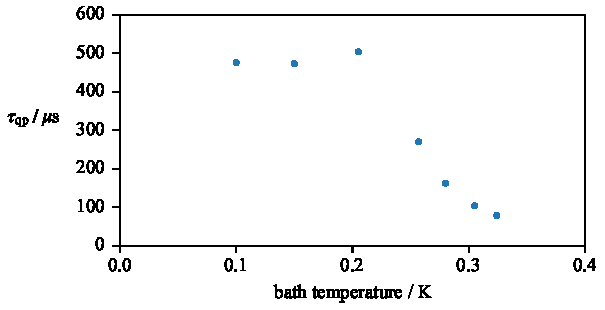
\includegraphics[width=\textwidth]{theory/tau_qp_vs_bath_temperature.pdf}
\caption
[The quasiparticle relaxation time versus bath temperature, showing saturation at low temperature.]
{
The quasiparticle relaxation time versus bath temperature, showing saturation at low temperature.
The device tested was an aluminum lumped-element KID.
Because the resonator bandwidth of these devices was comparable to the quasiparticle bandwidth, I performed these measurements at a frequency corresponding to a higher order resonance.
The relaxation time was extracted by fitting the exponential tail of the decay of the detector response to a pulse from an LED.
This data set was published in \textcite{McCarrick2014RSI}.
}
\label{fig:tau_qp_vs_bath_temperature}
\end{figure}

Figure~\ref{fig:tau_qp_vs_bath_temperature} shows measurements of the quasiparticle relaxation time versus bath temperature.
The device was an aluminum lumped-element KID tested inside a sealed aluminum package (a ``dark'' test) that was enclosed in a copper box containing a chunk of highly absorbent material.
The quasiparticle relaxation time saturates at \SI{0.5}{ms}.
This is the longest time we have observed in any experiment but is less than was achieved in the studies with better shielding.
In other experiments, we have regularly used aluminum or copper tape to seal the seams in packages but have not generally used other shielding.
Thus, even in our dark measurements, saturation is likely to be caused by background quasiparticle generation due to stray light.
In experiments where detectors are tested optically, the detectors are exposed the much higher ambient light level in the experimental volume, which is typically of order \SI{3}{K}.

It may be possible to measure the relaxation time indirectly, using steady-state measurements, but this requires careful interpretation.
Assume that constant power $\power$ excites quasiparticles with average energy close to $\gap$ in a superconductor occupying volume $\volume$.
Then, energy conservation yields
\begin{equation}
\power / \volume
  =
  \ssrate_\generation \gap
  =
  \left( \ssrate_\qprecombinationeff + \ssrate_\qpsingledecay \right) \gap
  =
  \gap \qpdensity / \tau,
\end{equation}
for some time $\tau$.
What is the relationship between $\tau$ and the relaxation time $\qprelaxationtime$?
Using Equation~\ref{eqn:rate_qpdensity}, 
\begin{equation}
\tau^{-1}
  =
  \frac{\ssrate_\qprecombinationeff + \ssrate_\qpsingledecay}{\ssqpdensity}
  =
  \qprecombinationeff \ssqpdensity + \qpsingledecay.
\end{equation}
Comparing this to
$\qprelaxationtime^{-1} = 2 \qprecombinationeff \ssqpdensity + \qpsingledecay$,
we see that the relationship between these times depends on the balance between pair recombination and single-quasiparticle decay.
In particular, the equation
$\power = \gap \ssqpdensity / \qprelaxationtime$
is correct \textit{only} when pair recombination is negligible.
In the opposite limit, where single-quasiparticle decay is negligible, the relationship is $\qprelaxationtime = \tau / 2$.
The factor of two arises from linearization of the quadratic recombination term.

This illustrates the confusing point that there are several ``lifetimes'' associated with the quasiparticle system.
The pair-recombination lifetime $\qprecombinationtime$ is not directly accessible to typical experiments using superconducting resonators.
Instead, these measure $\phonontrapping \qprecombinationtime$, the \textit{effective} lifetime of a single quasiparticle, extended due to the phonon trapping effect discussed in Section~\ref{sec:theory.quasiparticle.phonons}.
If single-quasiparticle decay is negligible than this latter quantity equals $\tau$ in the energy conservation equation above, and it could be measured in steady-state experiments.
The relaxation time $\qprelaxationtime$ is the quantity extracted from dynamic experiments that measure pulse decay or quasiparticle bandwidth.

\section{Resonators}
\label{sec:theory.resonator}

\subsection{A generic model for a shunt-coupled resonator}
\label{sec:theory.resonator.generic}

To understand KID response we need to understand how the behavior of a superconducting resonator will change when the surface impedance shifts in some region of the resonator.
A specific resonator geometry can be analyzed using circuit concepts such as capacitance and inductance.
However, since many different resonator geometries can be used for KIDs, I begin by introducing a generic resonator model.

The two relevant frequencies are the fixed readout tone frequency $\freadout_\readout$ and the variable resonance frequency $\freadout_\resonator$.
There are advantages to using lower readout frequencies, so KIDs are typically read out at their fundamental resonance.
Decreasing this frequency generally requires more area, which is a precious quantity at the focal plane of a telescope.

In order to compare resonators with very different resonance frequencies, it is more convenient to use dimensionless variables.
The fractional frequency shift is
$\shift = 1 - \freadout_\resonator / \freadout_\resonator^\zerotemp$,
where $\freadout_\resonator^\zerotemp$ is the resonance frequency in some fiducial state, such as temperature approaching zero.
One could measure this shift directly by tracking the resonance frequency in real time.
However, our readout system can measure this shift directly only by sweeping the readout tone across a resonance, as shown in Figures~\ref{fig:introduction_resonator_amplitude_phase}~and~\ref{fig:example_resonator_fit_amplitude_phase_and_normalized}.
This method is slow, and we thus measure $\shift$ only in steady-state.
A simple readout technique is to sweep a tone across a resonance,  use a resonator model to determine the resonance frequency, then  set a single tone at this frequency and sample rapidly.
With this technique, the dimensionless quantity measured when obtaining time-ordered data is the fractional frequency detuning
$\detuning = \freadout_\readout / \freadout_\resonator - 1$ of the resonance frequency from the readout frequency.
We set $\freadout_\readout$ as close to $\freadout_\resonator$ as the readout electronics allow, and typically $\detuning < \num{e-5}$.
The fractional frequency shift and the detuning are clearly closely related: to a very good approximation, a shift $\delta\shift$ corresponds to an equal shift $\delta\detuning$.
Generally, I will use $\shift$ when describing steady-state measurements and will use $\detuning$ when describing time-ordered data.
The signs of these parameters are chosen so that when the resonance frequency $\freadout_\resonator$ decreases, as it does under increasing illumination, the dimensionless parameter increases.

Additional parameters characterize the flow of energy in the resonator.
The quality factor of a resonator is defined to be the ratio of energy stored to the energy lost per radian of oscillation.
The latter equals the power lost divided by the angular oscillation frequency, which is typically very close to the resonance frequency, so the resonator quality factor is
\begin{equation}
\qf_\resonator
  =
  \frac{2 \pi \freadout_\resonator \energy_\mathrm{stored}}{\power_\mathrm{out}}.
\end{equation}
We distinguish between two mechanisms for energy loss: $\power_\mathrm{out}$ includes both dissipation internal to the resonator and loss due to radiation back onto the feedline:
\begin{equation}
\qf_\resonator^{-1}
  \equiv
  \loss_\resonator
  =
  \loss_\coupling + \loss_\internal
  \equiv
  \qf_\coupling^{-1} + \qf_\internal^{-1},
\end{equation}
where $\loss = \qf^{-1}$ is a notational convenience I will use repeatedly.
The inverse quality factor, which I refer to as a ``loss,'' is easier to work with, but quality factors are conventional.

Thus, the internal loss $\loss_\internal = \qf_\internal^{-1}$ characterizes dissipation in the resonator, and an increase in the quasiparticle number causes the internal loss to increase.
As discussed further in Chapter~\ref{chp:loss}, the internal loss also includes various non-ideal sources of loss, such as dissipation in dielectrics, radiation into free space, and dissipation caused by vortices in the superconducting film.
The coupling loss $\loss_\coupling = \qf_\coupling^{-1}$ characterizes the coupling strength between the resonator and the feedline.

An additional nuisance parameter, the asymmetry parameter $\asymmetry$, is necessary to characterize a commonly-occurring resonance asymmetry that can be caused either by parasitic coupling between the resonator and the feedline or by an impedance mismatch between the feedline and the transmission lines to which it connects~\autocite{Khalil2012JAP}.
For a symmetric resonance, $\asymmetry = 0$.

\todo[inline]{Understand coupling quality factor and radiation}
%This radiated power is assumed to propagate equally in both directions along the feedline until it is absorbed by matched resistive loads.
%Radiation propagating toward the low-noise amplifier is absorbed and amplified, while radiation propagating in the other direction is presumably absorbed by some matched load in the input chain.

KIDs are read out in the in the shunt-coupled configuration shown in Figure~\ref{fig:multiplexed_mkids_v1}.
It is convenient to express the measured transmission past the resonators in terms of the forward scattering parameter
$\forwardscattering = \voltage_2 / \voltage_1$,
where $\voltage_1$ and $\voltage_2$ are the complex voltages on the feedline of, respectively, the wave propagating toward the resonators and the wave arriving at the low-noise amplifier.
(The readout system actually records this quantity multiplied by the complex gain $G$ of the system:
$R_{21} = G \forwardscattering$.)
In terms of the parameters defined above, the forward scattering response due to one resonator is
\begin{equation}
\forwardscattering(\freadout_\readout, \freadout_\resonator, \loss_\internal, \loss_\coupling, \asymmetry)
  =
  1 - \frac{1 + \I \asymmetry}{1 + (\loss_\internal + 2 \I \detuning) / \loss_\coupling},
\label{eqn:forwardscattering}
\end{equation}
which is equivalent to the more familiar form~\autocite{Zmuidzinas2012ARCMP}
\begin{equation}
\forwardscattering(\freadout_\readout, \freadout_\resonator, \qf_\resonator, \qf_\coupling, \asymmetry)
  =
  1 - \frac{\qf_\resonator (1 + \I \asymmetry) / \qf_\coupling}{1 + 2 \I \qf_\resonator \detuning}.
\end{equation}
Figure~\ref{fig:example_resonator_fit_amplitude_phase_and_normalized} shows forward scattering data with the readout tone swept across the resonance frequency and a fit to Equation~\ref{eqn:forwardscattering}.
In time-ordered data collected at a fixed readout frequency the quantities that vary in time are $\loss_\internal$ and $\freadout_\resonator$ (and thus $\detuning$), while  
$\loss_\coupling$ and $\asymmetry$ do not vary.

\begin{figure}[tb]
\centering
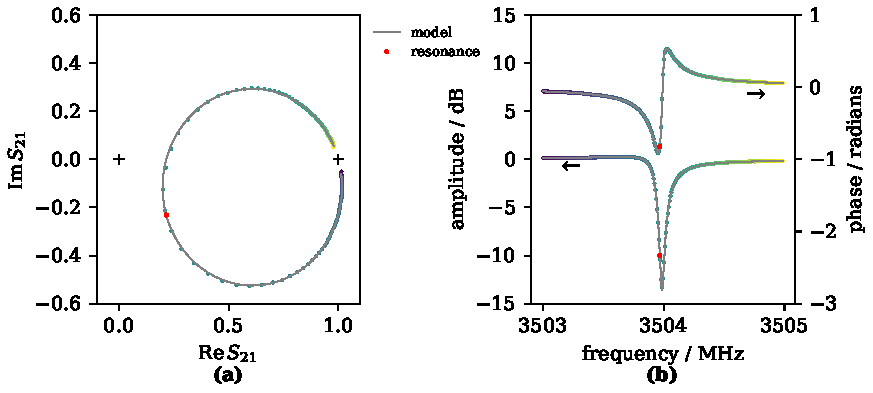
\includegraphics[width=\textwidth]{theory/example_resonator_fit_amplitude_phase_and_normalized.pdf}
\caption
[Complex transmission data from a frequency sweep across a resonator, normalized and fit to a resonator model.]
{
Complex transmission data from a frequency sweep across a resonance.
The resonator model given in Equation~\ref{eqn:forwardscattering} was fit to the data, and the points were normalized by dividing out the system gain.
The device is an aluminum CPW resonator with a resonance frequency near \SI{3.5}{GHz}.
In both panels, the purple (yellow) points correspond to the low (high) end of the frequency sweep, which spans \SI{2.0}{MHz}.
\textbf{(a)} 
The frequency sweep data and model in the complex $\forwardscattering$ plane.
The + symbols mark (0, 0) and (0, 1), which the model constrains the data to approach far from the resonance.
The internal loss is
$\loss_\internal = \num{8.9e-6} = 1 / \num{1.1e5}$,
and the coupling loss is
$\loss_\coupling = \num{3.2e-5} = 1 / \num{3.1e4}$.
This resonance has a relatively large value of the asymmetry parameter
$\asymmetry = 0.3$, which causes the resonance circle to be rotated and expanded.
\textbf{(b)} 
The same data and model plotted versus frequency, with amplitude on the left axis and phase on the right axis.
Because of the large asymmetry, the resonance frequency does not appear to be at the center of the amplitude or phase curves.
}
\label{fig:example_resonator_fit_amplitude_phase_and_normalized}
\end{figure}


\subsection{The effective kinetic inductance fraction}
\label{sec:theory.resonator.kifraction}

To model KID response, we must relate changes in the resonator parameters introduced above to changes in the film surface impedance in the region where quasiparticles are generated.
The two resonator geometries used in this thesis are lumped-element resonators and quarter-wave transmission-line resonators.

We begin with the simpler case of a lumped-element resonator. 
Figures~\ref{fig:loss.experiment}~and~\ref{fig:measuring.experiment} show drawings of aluminum lumped-element resonators, which consist of a meandered inductive trace and an interdigital capacitor that are both electrically short at the resonance frequency.
For these devices, the resonance frequency is
$\freadout_\resonator
  =
  (2 \pi)^{-1} (\inductance \capacitance)^{-1/2}$
where $\inductance$ is the total inductance of the resonator and $\capacitance$ is its total capacitance.
The total inductance
$\inductance = \inductance_\geometric + \inductance_\kinetic$
is the sum of the geometric inductance $\inductance_\geometric$ and the kinetic inductance $\inductance_\kinetic$, where $\reactance_\surface = 2 \pi \freadout \inductance_\kinetic$.
The response to an inductance shift in some region is weighted by the square of the current in that region~\autocite{Mazin2005,Gao2008}.
For these resonators, the current is approximately constant along the inductive meander and is very small in the capacitor.
Assume that quasiparticles cause a homogeneous shift in the surface impedance of the inductor.
Then, a small shift in the kinetic inductance
$\inductance_\kinetic - \inductance_\kinetic(0)$ from the zero-temperature value $\inductance_\kinetic(0)$ produces a new resonance frequency
\begin{equation}
\freadout_\resonator
  \approx
  \freadout_\resonator(0)
  \left( 1 - \frac{\inductance_\kinetic - \inductance_\kinetic(0)}{2 [\inductance_\geometric + \inductance_\kinetic(0)]} \right)
  \equiv
  \freadout_\resonator(0)
  \left( 1 - \frac{\kifraction}{2} \frac{\inductance_\kinetic - \inductance_\kinetic(0)}{\inductance_\kinetic(0)} \right).
\end{equation}
Here, the effective kinetic inductance fraction is
\begin{equation}
\kifraction
  =
  \frac{\inductance_\kinetic(0)}{\inductance_\geometric + \inductance_\kinetic(0)}
  =
  \frac{\reactance_\surface(0)}{\reactance_\geometric + \reactance_\surface(0)},
\end{equation}
where $\reactance_\geometric = 2 \pi \freadout \inductance_\geometric$.
In this simple case, the effective kinetic inductance fraction actually equals the ratio of the kinetic inductance to the total inductance, but this is not true when the surface impedance does not shift homogeneously.

The corresponding fractional frequency shift is
\begin{equation}
\shift
  =
  \frac{\kifraction}{2} \frac{\reactance_\surface - \reactance_\surface(0)}{\reactance_\surface(0)}.
\end{equation}
The approximations used here should be quite good in practice: for the lumped-element detectors discussed
in Chapter~\ref{chp:sensitivity}, the total fractional frequency shift between no illumination and very high illumination is $\shift < \num{e-3}$.
Thus, all three of the frequencies $\freadout_\readout$, $\freadout_\resonator$, and $\freadout_\resonator(0)$ are very close to each other so $\kifraction$ can be treated as a constant.

Attributing all dissipation that occurs within the film to quasiparticles, the quasiparticle loss is~\autocite{Zmuidzinas2012ARCMP}
\begin{equation}
\loss_\quasiparticle
  =
  \qf_\quasiparticle^{-1}
  =
  \kifraction \frac{\resistance_\surface}{\reactance_\surface(0)}.
\label{eqn:resonator.loss_quasiparticle}
\end{equation}

The hybrid co-planar waveguide (CPW) KIDs discussed in Chapter~\ref{chp:multichroic} consist of two different sections of CPW in series.
The section closest to the transmission line is made from a high-gap superconductor in which no quasiparticles are excited.
The other section consists of an aluminum center strip that is electrically connected to the high-gap superconductor center strip at one end and to the ground plane at the other end.
The total length is a quarter wavelength at the fundamental resonance frequency.
The quasiparticles are confined to the aluminum region of the center strip, called the active region, where the current is highest.
Thus, only the surface impedance in the active region is altered.
For these resonators we can use the same equations as above with the geometric complications folded into the effective kinetic inductance fraction~\autocite{Gao2008}.
\todo[inline]{Incorporate Jiansong's work on hybrid resonators and on transmission-line resonators with an arbitrary terminating impedance.}

\section{Detector response and responsivity}
\label{sec:theory.response}

In the quasiparticle number model, the response of a KID to light is determined by the following chain of relations.
First, the optical power absorbed by the detector is the product of the incident power and the optical efficiency.
Second, the absorbed power, photon energy, and material parameters determine the optical quasiparticle generation rate.
Third, the total quasiparticle generation rate and the various quasiparticle decay channels determine the quasiparticle number.
Fourth, the quasiparticle number determines the complex conductivity.
Fifth, the complex conductivity and resonator geometry determine the surface impedance.
Sixth, the surface impedance and resonator geometry determine the resonance frequency and quality factors of the resonator.
Seventh, the resonator parameters and readout tone frequency determine the forward scattering parameter that is measured by the readout electronics.
This is a long list, but most of these relationships turn out to be simple.
I use \textit{response} to mean the shift in some quantity from the zero-illumination case and use \textit{responsivity} to mean the derivative at a particular operation point.


\subsection{Photodetection}
\label{sec:theory.response.photodetection}

If the incident optical power at some reference plane is $\power_\incident$ and the optical power absorbed in the active region of the detector is $\power_\optical$, then the optical efficiency $\efficiency_\incident$ for power at this plane relates them:
\begin{equation}
\label{eqn:photodetection.response}
\power_\optical = \efficiency_\incident \power_\incident.
\end{equation}
The responsivity is
\begin{equation}
\label{eqn:photodetection.responsivity}
\pdv{\power_\optical}{\power_\incident}
  =
  \efficiency_\incident.
\end{equation}
The process by which the absorption occurs depends on the detector architecture.
In the lumped-element KIDs discussed in Chapters~\ref{chp:loss} and \ref{chp:sensitivity}, millimeter-wave light is concentrated by a feed horn onto a meandering inductor that forms the sensing region of the detector.
For the co-planar waveguide KIDs discussed in Chapter~\ref{chp:multichroic}, the light is coupled through a feedhorn into a planar ortho-mode transducer (OMT) antenna, and routed through millimeter-wave circuitry into the high-current (shorted) end of a quarter-wave CPW resonator.
\todo[inline]{Discuss conductivity just above cutoff}
\begin{comment}
For frequencies $\foptical$ more than a few times the optical cutoff frequency $\foptical_\cutoff = 2 \gap / \planck$,
$\reconductivity(\foptical) = \normalconductivity$
and
$\imconductivity(\foptical) = 0$.
For frequencies closer to the gap, the Mattis-Bardeen equations should be used to obtain more accurate results.
\end{comment}
Chapter~\ref{chp:sensitivity} discusses a method for obtaining the optical efficiency, and thus the absorbed power, from measurements of the noise level.
\todo[inline]{Plot $\conductivity$ for $\foptical > \foptical_\cutoff$ and discuss.}
\todo[inline]{Discuss LEKID impedance matching.}
\todo[inline]{Any difference between A normal to film and A in plane?}
\todo[inline]{Discuss Popel exact thin-film solution}


\begin{figure}[htb]
\centering
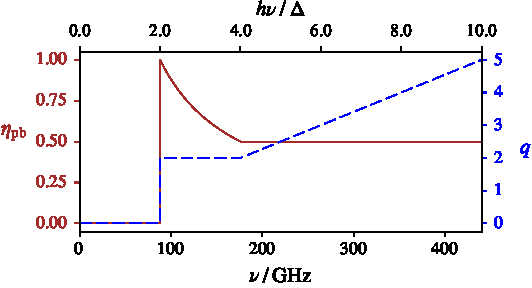
\includegraphics[width=0.9\textwidth]{theory/quasiparticles_per_photon_and_pairbreaking_efficiency.pdf}
\caption
[The number of quasiparticles excited per photon and the pair-breaking efficiency versus photon frequency.]
{A sketch of the number of quasiparticles excited per photon and the pair-breaking efficiency, both plotted versus photon frequency and photon energy in units of the gap.
The values on the upper horizontal axis are universal, while the frequency values on the lower horizontal axis are calculated for a BCS superconductor with the bulk aluminum $\tc = \SI{1.2}{K}$.
For $\planck \foptical > 4 \gap$, the phonon trapping factor $\phonontrapping$ affects the fraction of photon energy that is converted into quasiparticles.
Figure~4 of \textcite{Guruswamy2014SUST} shows a theoretical calculation of $\pbefficiency$ that suggests $0.4 < \pbefficiency < 0.6$ at higher energies.
The choice made here of $\pbefficiency = 0.5$ corresponds to a phonon trapping factor $\phonontrapping \sim 3$.
Figure~2 of \textcite{deVisser2015APL} shows a measurement of $\pbefficiency$ that qualitatively agrees with this figure.
\todo[inline]{Re-create this pair-breaking plot with harmonized fiducials.}}
\label{fig:quasiparticles_per_photon_and_pairbreaking_efficiency}
\end{figure}

\subsection{Optical quasiparticle generation}
\label{sec:theory.response.generation}

As the optical power $\power_\optical$ is absorbed in the active region of the KID, each absorbed photon generates $\qpperphoton \ge 2$ quasiparticles on average.
The number of quasiparticles excited by a given photon with $\planck \foptical \ge 4 \gap$ may vary, and for very high-energy photons the details of the down-conversion process are complex~\autocite{Kozorezov2000PRB}.
For KIDs designed to resolve the energy of single photons, the variation of the created quasiparticle number is a fundamental source of noise~\autocite{Mazin2005}.
However, this variation is not important for photometric detectors, which do not resolve individual photon arrivals.
The variance of the quasiparticle number under steady illumination will turn out to be linear in $\qpperphoton$, so we can obtain correct results for the noise while considering only the average number of excitations per photon.
Most of the measurements presented here are made using photon energies $\planck \foptical \gtrsim 2 \gap$, where $\qpperphoton = 2$ exactly.

In the KID literature one often encounters the pair-breaking efficiency
\begin{equation}
\pbefficiency
  =
  \frac{\qpperphoton \expval{\energy_\quasiparticle}}{\planck \foptical}
  \approx
  \frac{\qpperphoton \gap}{\planck \foptical},
\label{eqn:pbefficiency}
\end{equation}
where $\expval{\energy_\quasiparticle} \gtrsim \gap$ is the average quasiparticle energy.
Approximately, $\pbefficiency$ is the fraction of photon energy that is converted into energy in the steady-state quasiparticle system.
Figure~\ref{fig:quasiparticles_per_photon_and_pairbreaking_efficiency} is a sketch of $\qpperphoton$ and $\pbefficiency$ for photon energies $\planck \foptical$ near the spectroscopic gap.
For $\planck \foptical < 2 \gap$, no quasiparticles are excited because the excitations must be created in pairs.
For $2 \gap < \planck \foptical < 4 \gap$, each photon excites exactly two quasiparticles and the remaining energy is converted into phonons that do not have sufficient energy to break additional pairs.
For $4 \gap < \planck \foptical$ each photon may break more than one pair, and approximately half the photon energy is converted into quasiparticles.
The value $\pbefficiency \approx 0.6$ is commonly used.
However, as discussed in detail by \textcite{Guruswamy2014SUST}, $\pbefficiency$ depends on the details of phonon trapping: it is lower when the phonon trapping factor is lower because a high-energy phonon is more likely to escape before depositing its energy in the quasiparticle system.

Thus, if a detector absorbs optical power $\power_\optical$ from photons with frequency $\foptical$, the optical quasiparticle generation rate is
\begin{equation}
\Rate_\optical
  =
  \frac{\qpperphoton \power_\optical}{\planck \foptical}
  =
  \frac{\pbefficiency \power_\optical}{\gap},
\label{eqn:optical_generation.response}
\end{equation}
and the responsivity is
\begin{equation}
\pdv{\Rate_\optical}{\power_\optical}
  =
  \frac{\qpperphoton}{\planck \foptical}
  =
  \frac{\pbefficiency}{\gap}.
\label{eqn:optical_generation.responsivity}
\end{equation}


\subsection{Quasiparticle number}
\label{sec:theory.response.qpnumber}

It is difficult to uniformly illuminate the active (sensing) region of a KID, so the generation rate is likely to vary with position.
Nevertheless, we now assume that diffusion  equalizes the quasiparticle density within the active region of the resonator.
This allows us to use the results of Section~\ref{sec:theory.qpnumber} with the quasiparticle density replaced by the quasiparticle number
$\qpnumber = \volume \qpdensity$,
where $\volume$ is the active volume.
The quasiparticle number depends on the total generation rate
$\Rate_\generation = \rate_\generation \volume$,
which accounts for all generation sources, such as absorption of optical photons, readout photons, and thermal phonons:
\begin{equation}
\Rate_\generation
  =
  \Rate_\optical + \Rate_\readout + \Rate_\thermal.
\end{equation}
We expect these rates to be approximately independent so that
$
\pdv*{\qpnumber}{\Rate_\optical}
  =
  \pdv*{\qpnumber}{\Rate_\generation}.
$

The steady-state quasiparticle number is given by Equation~\ref{eqn:ssqpdensity} multiplied by $\volume$:
\begin{equation}
\ssqpnumber
  = 
  \left( \left(\frac{\volume \qpsingledecay}{2 \qprecombinationeff}\right)^2
  + \frac{\volume \ssRate_\generation}{\qprecombinationeff} \right)^{1/2}
  - \frac{\volume \qpsingledecay}{2 \qprecombinationeff},
\label{eqn:qpnumber.response}
\end{equation}
with
$\ssqpnumber = (\volume \ssRate_\generation / \qprecombinationeff)^{1/2}$
when single-quasiparticle decay is negligible.

The corresponding responsivity to slow perturbations around this number is given by Equation~\ref{eqn:qprelaxationtime}:
\begin{equation}
\pdv{\ssqpnumber}{\ssRate_\generation}
  =
  \qprelaxationtime
  =
  \left( \frac{2 \qprecombinationeff \ssqpnumber}{\volume} + \qpsingledecay \right)^{-1}
  =
  \left( \frac{2 \ssRate_\generation}{\ssqpnumber} - \qpsingledecay \right)^{-1}
  =
  \left( \frac{4 \qprecombinationeff \ssRate_\generation}{\volume} + \qpsingledecay^2 \right)^{-1/2}.
\label{eqn:qpnumber.responsivity}
\end{equation}
This equation is valid only for perturbations that occur on time scales much larger than $\qprelaxationtime$.
To describe faster perturbations, we may define
$\delta\qpnumber(\time) = \qpnumber(\time) - \ssqpnumber$
and 
$\delta\Rate_\generation(\time) = \Rate_\generation(\time) - \ssRate_\generation$, and the corresponding Fourier transforms
\begin{equation}
\delta\qpnumber(\time)
  =
  \int_{-\infty}^\infty \dd{\faudio}
  \exp(2 \pi \I \faudio \time) \, \delta\qpnumber(\faudio)
  \qqtext{and}
\delta\Rate_\generation(\time)
  =
  \int_{-\infty}^\infty \dd{\faudio}
  \exp(2 \pi \I \faudio \time) \, \delta\Rate_\generation(\faudio).
\end{equation}
The solution is just Equation~\ref{eqn:delta_qpdensity_frequency} multiplied by the active volume $\volume$:
\begin{equation}
\delta\qpnumber(\faudio)
  =
  \frac{\qprelaxationtime}{1 + 2 \pi \I \faudio \qprelaxationtime} \delta\Rate_\generation(\faudio).
\label{eqn:delta_qpnumber_frequency}
\end{equation}
As shown above, the optical generation rate $\Rate_\optical$ is proportional to the absorbed optical power $\power_\optical$;
as shown below, the quantities measured by the KID readout system are proportional to $\qpnumber$.
Thus, when optical generation dominates, we expect the detector response to go as $\power_\optical^{1/2}$ and the responsivity to go as $\power_\optical^{-1/2}$.
The data shown in Figure~\ref{fig:measuring.results} behave according to this prediction.


\subsection{Complex conductivity}
\label{sec:theory.response.complex_conductivity}

The complex conductivity $\conductivity$ for an arbitrary quasiparticle occupancy $\qpoccupancy(\energy)$ is determined by the Mattis-Bardeen equations, given in Section~\ref{sec:theory.electrodynamics.mattis-bardeen}.
KIDs should be operated at
$\temperature \ll \tc$
and should be designed so that, under the highest expected illumination, both real and imaginary parts of the change in the complex conductivity remain small compared to the zero temperature value:
\begin{equation}
\frac{\conductivity - \conductivity(0)}{\imconductivity(0)}
  =
  \frac{\braket*{\responseqpoccupancy_{\reconductivity}}{\qpoccupancy} - \I \braket*{\responseqpoccupancy_{\imconductivity}}{\qpoccupancy}}{\imconductivity(0)},
\end{equation}
where
$\imconductivity(0)
  =
  \pi \gap_\zerotemp \normalconductivity / \planck \freadout$.
To use analytic results for the conductivity response, I will assume that $\qpoccupancy$ remains sufficiently small that the first-order approximations discussed in Section~\ref{sec:theory.perturbation} and Appendix~\ref{chp:first-order_response} remain accurate.
As shown by Figures~\ref{fig:responseqpoccupancy_conductivity_f_mc} and~\ref{fig:responseqpoccupancy_conductivity_f_1p}, the response functions for the components of the conductivity are quite different, so an arbitrary perturbation to the occupancy could cause unrelated shifts in $\reconductivity$ and $\imconductivity$.
We avoid this complication using the assumption, also introduced in Section~\ref{sec:theory.perturbation},
that perturbations $\delta\qpoccupancy$ are proportional to $\ssqpoccupancy$.
In this case, the responsivity is 
\begin{equation}
\frac{\delta\conductivity}{\delta\qpnumber}
  =
  \frac{\braket*{\responseqpoccupancy_{\conductivity}}{\delta\qpoccupancy}}{\braket*{\responseqpoccupancy_{\qpnumber}}{\delta\qpoccupancy}}
  =
  \frac{\braket*{\responseqpoccupancy_{\conductivity}}{\ssqpoccupancy}}{\braket*{\responseqpoccupancy_{\qpnumber}}{\ssqpoccupancy}}
  =
  \frac{\conductivity - \conductivity(0)}{\qpnumber}.
\end{equation}
Taking real and imaginary parts gives
\begin{equation}
\frac{\delta\reconductivity}{\delta\qpnumber}
  =
  \frac{\braket*{\responseqpoccupancy_{\reconductivity}}{\ssqpoccupancy}}{\braket*{\responseqpoccupancy_{\qpnumber}}{\ssqpoccupancy}}
\qqtext{and}
\frac{\delta\imconductivity}{\delta\qpnumber}
  =
\frac{\braket*{\responseqpoccupancy_{\imconductivity}}{\ssqpoccupancy}}{\braket*{\responseqpoccupancy_{\qpnumber}}{\ssqpoccupancy}}.
\label{eqn:delta_conductivity_delta_qpnumber}
\end{equation}
When the quasiparticle number increases, the real part of the conductivity increases and the imaginary part decreases.

\begin{figure}[htb]
\centering
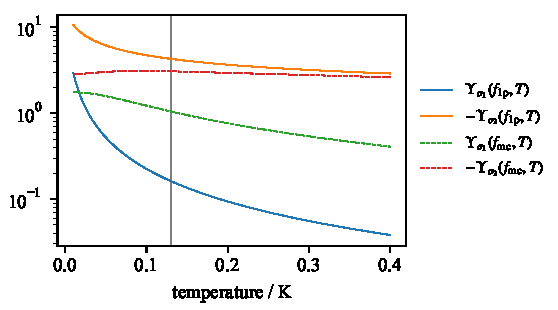
\includegraphics[width=0.8\textwidth]{theory/normresponse_conductivity_thermal.pdf}
\caption[The normalized response ratios of the real and imaginary conductivity to the thermal quasiparticle density.]
{
The normalized response ratios of the real and imaginary conductivity to the thermal quasiparticle density.
The vertical gray line marks the fiducial bath temperature, assuming fiducial values for aluminum.
}
\label{fig:normresponse_conductivity_thermal}
\end{figure}

We can express the ratios of the real and imaginary components of the conductivity response to the quasiparticle density response in dimensionless form (using the same normalization constants, up to a sign, as \textcite{Zmuidzinas2012ARCMP}):
\begin{align}
\begin{split}
\normresponse_{\reconductivity}[\qpoccupancy]
  &=
  \frac{\braket*{\responseqpoccupancy_{\reconductivity}}{\qpoccupancy} / \imconductivity(0)}{\braket*{\responseqpoccupancy_{\qpdensity}}{\qpoccupancy} / 2 \ssdos \gap_\zerotemp}; \\
\normresponse_{\imconductivity}[\qpoccupancy]
  &=
  \frac{\braket*{\responseqpoccupancy_{\imconductivity}}{\qpoccupancy} / \imconductivity(0)}{\braket*{\responseqpoccupancy_{\qpdensity}}{\qpoccupancy} / 2 \ssdos \gap_\zerotemp}.
\end{split}
\label{eqn:normresponse_conductivity}
\end{align}
These functions must be calculated numerically for an arbitrary occupancy.
For a thermal occupancy we can use Equations~\ref{eqn:qpdensity_thermal}, \ref{eqn:responseqpoccupancy_reconductivity_thermal}, and \ref{eqn:responseqpoccupancy_imconductivity_thermal} to obtain
\begin{equation}
\normresponse_{\reconductivity}(\temperature)
  =
  \left( \frac{8 \gap_\zerotemp}{\pi^3 \kb \temperature} \right)^{1/2}
  \sinh \left( \frac{\planck \freadout}{2 \kb \temperature} \right)
  K_0 \left( \frac{\planck \freadout}{2 \kb \temperature} \right)
\label{eqn:normresponse_reconductivity_thermal}
\end{equation}
and
\begin{equation}
\normresponse_{\imconductivity}(\temperature)
  =
  - \left[
  1 + \left( \frac{2 \gap_\zerotemp}{\pi \kb \temperature} \right)^{1/2}
  \exp \left( -\frac{\planck \freadout}{2 \kb \temperature} \right)
  I_0 \left( \frac{\planck \freadout}{2 \kb \temperature} \right)
  \right].
\label{eqn:normresponse_imconductivity_thermal}
\end{equation}
These functions are plotted in Figure~\ref{fig:normresponse_conductivity_thermal} for the fiducial readout frequencies.
The imaginary part of the conductivity responds much more to quasiparticles than the real part.
Additionally, at the fiducial bath temperature, the ratio of the reactive response to the dissipative response
$\jonasbeta(\temperature, \freadout)
  \equiv
  |\normresponse_{\imconductivity}(\temperature, \freadout) / \normresponse_{\reconductivity}(\temperature, \freadout)|$
is nearly 30 at $\freadout_\singlepol$, while it is only about 3 at $\freadout_\multichroic$.
These predictions will turn out to be approximately true even under optical illumination.

Finally, combining Equation~\ref{eqn:delta_conductivity_delta_qpnumber} with Equation~\ref{eqn:normresponse_conductivity} gives
\begin{equation}
\pdv{\reconductivity}{\qpnumber}
  =
  \frac{\imconductivity(0)}{2 \ssdos \gap_\zerotemp \volume} \normresponse_{\reconductivity}[\qpoccupancy]
\label{eqn:delta_reconductivity_delta_qpnumber_normresponse}
\end{equation}
and
\begin{equation}
\pdv{\imconductivity}{\qpnumber}
  =
  \frac{\imconductivity(0)}{2 \ssdos \gap_\zerotemp \volume} \normresponse_{\imconductivity}[\qpoccupancy].
\label{eqn:delta_imconductivity_delta_qpnumber_normresponse}
\end{equation}
Because $\normresponse_{\imconductivity}$ is negative, the imaginary part of the complex conductivity decreases with increasing quasiparticle number.


\subsection{Surface impedance}
\label{sec:theory.response.surface_impedance}

Taking derivatives of the first-order expressions in Equation~\ref{eqn:surface_resistance_and_reactance_shift} leads to
\begin{equation}
\pdv{\resistance_\surface}{\reconductivity}
  =
  \frac{\surfimpexp \reactance_\surface(0)}{\imconductivity(0)},
\end{equation}
and
\begin{equation}
\pdv{\reactance_\surface}{\imconductivity}
  =
  - \frac{\surfimpexp \reactance_\surface(0)}{\imconductivity(0)}.
\end{equation}


\subsection{Resonator parameters}
\label{sec:theory.response.resonator}

From Section~\ref{sec:theory.resonator}, we have
\begin{equation}
\loss_\quasiparticle
  =
  \frac{\kifraction \resistance_\surface}{\reactance_\surface(0)}
\end{equation}
and
\begin{equation}
\shift
  =
  \frac{\kifraction}{2} \frac{\reactance_\surface - \reactance_\surface(0)}{\reactance_\surface(0)}.
\end{equation}
The responsivities are thus
\begin{equation}
\pdv{\loss_\quasiparticle}{\resistance_\surface}
  =
  \frac{\kifraction}{\reactance_\surface(0)}
\label{eqn:delta_loss_internal_delta_resistance_surface}
\end{equation}
and
\begin{equation}
\pdv{\detuning}{\reactance_\surface}
  =
  \pdv{\shift}{\reactance_\surface}
  =
  \frac{\kifraction}{2 \reactance_\surface(0)}.
\label{eqn:delta_detuning_delta_reactance_surface}
\end{equation}


\begin{figure}[htb]
\centering
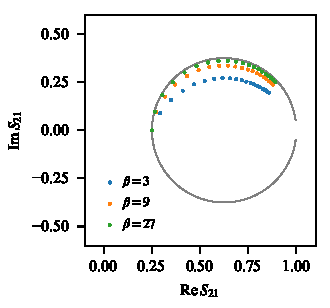
\includegraphics[width=0.8\textwidth]{theory/s21_response.pdf}
\caption
[Theoretical predictions for the $\forwardscattering$ response to an increase in the quasiparticle number.]
{
Theoretical predictions for the $\forwardscattering$ response to an increase in the quasiparticle number.
The parameter
$\jonasbeta
  =
  - \normresponse_{\imconductivity} / \normresponse_{\reconductivity}
  =
  2 \delta\detuning / \delta\loss_\internal$
determines the trajectory of the response in the complex $\forwardscattering$ plane.
}
\label{fig:s21_response}
\end{figure}

\subsection{The forward scattering parameter}
\label{sec:theory.response.forwardscattering}

\todo[inline]{Move this content to the resonator section}
When the resonator parameters $\loss_\internal(\time)$ and $\detuning(\time)$ change slowly, the $\forwardscattering$ response is given by the partial derivatives in the obvious way:
\begin{equation}
\adiabatici
  \equiv
  \pdv{\forwardscattering}{\loss_\internal}
  =
  \frac{(1 + \I \asymmetry) \loss_\coupling}{(\loss_\coupling + \loss_\internal + 2 \I \detuning)^2}
  =
  \frac{(1 - \forwardscattering)^2}{(1 + \I \asymmetry) \loss_\coupling}
\end{equation}
and
\begin{equation}
\adiabaticx
  \equiv
  \pdv{\forwardscattering}{\detuning} 
  =
  2 \I \pdv{\forwardscattering}{\loss_\internal}
  =
    \frac{(2 \I - 2 \asymmetry) \loss_\coupling}{(\loss_\coupling + \loss_\internal + 2 \I \detuning)^2}
  =
  \frac{2 \I (1 - \forwardscattering)^2}{(1 + \I \asymmetry) \loss_\coupling}.
\end{equation}
Factoring these equations shows that the response is maximized when $\detuning = 0$ and when $\loss_\internal = \loss_\coupling$~\autocite{Zmuidzinas2012ARCMP}.
When $\detuning = 0$ and $\asymmetry = 0$, $\forwardscattering$  and $\adiabatici$ are purely real, while $\adiabaticx$ is purely imaginary.
The partial derivatives are orthogonal even when these conditions are not satisfied, and they correspond to directions that are tangent to and normal to the resonance circle.

The forward scattering parameter does not react instantly to changes in the resonator parameters, and this effect can be accounted for using a resonator transfer function $\restransfer$.
When $\detuning = 0$, the Fourier domain transfer function is just a single-pole low-pass filter with the same shape as the resonator~\autocite{Gao2008,Zmuidzinas2012ARCMP}:
$\restransfer(\faudio)
  =
  \left( 1 + \I \faudio / \faudio_\resonator \right)^{-1}$,
where $\faudio$ is the signal frequency and
$\faudio_\resonator = \freadout_\resonator \loss_\resonator / 2$
is the resonator bandwidth, which is half its linewidth.
The resonator bandwidth is generally much larger than the quasiparticle bandwidth.
However, the lumped-element resonators discussed in Chapters~\ref{chp:loss}~and~\ref{chp:sensitivity} have unusually low resonance frequencies and low internal loss, and for these resonators the two bandwidths are similar.


\subsection{Summary}
\label{sec:theory.response.summary}

\begin{figure}[htb]
\centering
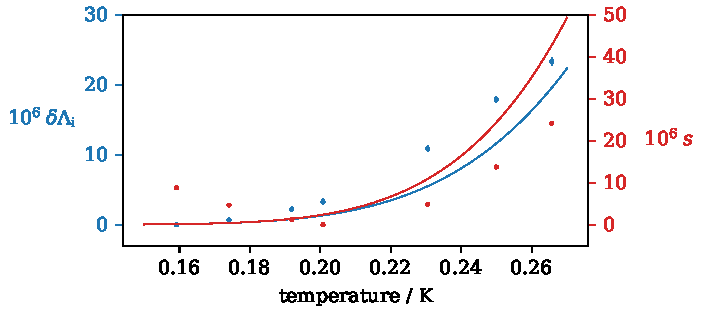
\includegraphics[width=\textwidth]{theory/mkidarray02_chosen_one_di_and_s_versus_temperature.pdf}
\caption[MKIDArray02-0001: the internal loss and fractional frequency shift versus temperature for a multichroic \SI{3410}{MHz} resonator.]
{
MKIDArray02-0001: the change in internal loss and fractional frequency shift versus temperature for a multichroic \SI{3410}{MHz} resonator.
Here,
$\delta\loss_\internal = \loss_\internal - \loss_\internal^\mathrm{min}$.
The points are the measured data, and the corresponding lines are Equation~\ref{eqn:ssloss_quasiparticle} for the internal loss and Equation~\ref{eqn:ssshift} for the fractional frequency shift, both evaluated using fiducial parameters and an effective kinetic inductance fraction $\kifraction = 0.2$.
}
\label{fig:mkidarray02_chosen_one_di_and_s_versus_temperature}
\end{figure}

We can now combine equations from the preceding sections to obtain the detector response and responsivity.
The steady-state quasiparticle loss is
\begin{equation}
\ssloss_\quasiparticle
  =
  \frac{\kifraction}{\reactance_\surface(0)}
  \frac{\surfimpexp \reactance_\surface(0)}{\imconductivity(0)}
  \ssreconductivity
  =
  \frac{\kifraction \surfimpexp}{\imconductivity(0)}
  \braket*{\responseqpoccupancy_{\reconductivity}}{\ssqpoccupancy},
\label{eqn:ssloss_quasiparticle}
\end{equation}
and the steady-state fractional frequency shift is
\begin{equation}
\ssshift
  =
  \frac{\kifraction}{2 \reactance_\surface(0)}
  \left( -\frac{\surfimpexp \reactance_\surface(0)}{\imconductivity(0)} \right)
  \left[ \ssimconductivity - \imconductivity(0) \right]
  =
  -\frac{\kifraction \surfimpexp}{2 \imconductivity(0)}
  \braket*{\responseqpoccupancy_{\imconductivity}}{\ssqpoccupancy}.
\label{eqn:ssshift}
\end{equation}
(Recall that $\responseqpoccupancy_{\imconductivity}$ is negative.)
Figure~\ref{fig:mkidarray02_chosen_one_di_and_s_versus_temperature} shows the above equations, calculated for a thermal occupancy, along with data from a multichroic CPW KID.
The theory and data agree within about a factor of two, but the behavior of this resonator appears to be significantly affected by two-level systems in nearby dielectrics.
(See Section~\ref{sec:loss.dielectrics} and Section~\ref{sec:multichroic.mkidarray02}.)

To describe time-dependent perturbations around these values, caused by $\delta\qpoccupancy(\time)$, we can write
\begin{align}
\begin{split}
\delta\loss_\quasiparticle(\time)
  =
  \pdv{\loss_\quasiparticle}{\resistance_\surface}
  \pdv{\resistance_\surface}{\reconductivity}
  \delta\reconductivity(\time)
  &=
  \frac{\kifraction \surfimpexp}{\imconductivity(0)}
  \braket*{\responseqpoccupancy_{\reconductivity}}{\delta\qpoccupancy(\time)} \\
  &=
  \frac{\kifraction \surfimpexp}{\imconductivity(0)}
  \frac
  {\braket*{\responseqpoccupancy_{\reconductivity}}{\ssqpoccupancy}}
  {\braket*{\responseqpoccupancy_{\qpnumber}}{\ssqpoccupancy}}
  \braket*{\responseqpoccupancy_{\qpnumber}}{\delta\qpoccupancy(\time)} \\
  &=
  \frac{\kifraction \surfimpexp \ssnormresponse_{\reconductivity}}{2 \ssdos \gap_\zerotemp \volume} \delta\qpnumber(\time),
\end{split}
\end{align}
where $\ssnormresponse_{\reconductivity} = \normresponse_{\reconductivity}[\ssqpoccupancy]$, and
\begin{align}
\begin{split}
\delta\detuning(\time)
  =
  \pdv{\detuning}{\reactance_\surface}
  \pdv{\reactance_\surface}{\imconductivity}
  \delta\imconductivity(\time)
  &=
  -\frac{\kifraction \surfimpexp}{2 \imconductivity(0)}
  \braket*{\responseqpoccupancy_{\imconductivity}}{\delta\qpoccupancy(\time)} \\
  &=
  -\frac{\kifraction \surfimpexp}{2 \imconductivity(0)}
  \frac
  {\braket*{\responseqpoccupancy_{\imconductivity}}{\ssqpoccupancy}}
  {\braket*{\responseqpoccupancy_{\qpnumber}}{\ssqpoccupancy}}
  \braket*{\responseqpoccupancy_{\qpnumber}}{\delta\qpoccupancy(\time)} \\
  &=
  -\frac{\kifraction \surfimpexp \ssnormresponse_{\imconductivity}}{4 \ssdos \gap_\zerotemp \volume} \delta\qpnumber(\time),
\end{split}
\end{align}
where
$\ssnormresponse_{\imconductivity} = \normresponse_{\imconductivity}[\ssqpoccupancy]$
and 
$\delta\imconductivity = \imconductivity - \ssimconductivity$.
Since $\normresponse_{\imconductivity}$ is negative, both $\delta\loss_\internal$ and $\delta\detuning$ increase when the quasiparticle number increases.
Finally, we can relate the quasiparticle number to the generation rate, which is proportional to the absorbed power.
The steady-state values will be set by the steady-state generation rate $\ssRate_\generation$.
As above, consider small perturbations
$\delta\Rate_\generation(\time)
  =
  \Rate_\generation(\time) - \ssRate_\generation$ around this rate.
Then, given the frequency-domain perturbation $\delta\Rate_\generation(\faudio)$, the frequency-domain quasiparticle loss response is
\begin{equation}
\delta\loss_\quasiparticle(\faudio)
  =
  \frac{\kifraction \surfimpexp \ssnormresponse_{\reconductivity}}{2 \ssdos \gap_\zerotemp \volume}
  \frac{\qprelaxationtime}{1 + 2 \pi \I \faudio \qprelaxationtime}
  \delta\Rate_\generation(\faudio).
\end{equation}
Similarly, the frequency-domain detuning response is
\begin{equation}
\delta\detuning(\faudio)
  =
  -\frac{\kifraction \surfimpexp \ssnormresponse_{\imconductivity}}{4 \ssdos \gap_\zerotemp \volume}
  \frac{\qprelaxationtime}{1 + 2 \pi \I \faudio \qprelaxationtime}
  \delta\Rate_\generation(\faudio).
\end{equation}
When the perturbations in the generation rate are due to incident optical power $\power_\incident$, we can use
\begin{equation}
\delta\Rate_\generation(\faudio)
  =
  \frac{\qpperphoton \efficiency_\incident}{\planck \foptical}
  \delta\power_\incident(\faudio).
\end{equation}
These equations describe the quasiparticle loss, but the resonator behavior depends on the total internal loss.
Using
$\loss_\quasiparticle = \qpfraction \loss_\internal$,
the forward scattering response can be included straightforwardly.
As discussed below, we usually use the resonator model to obtain $\loss_\internal$ and $\detuning$, which is more convenient than working with $\forwardscattering$.
\todo[inline]{Discuss forwardscattering response}
\todo[inline]{Combine the two adiabatic response guys into a single guy}


\subsection{Time-ordered data}
\label{sec:theory.response.time-ordered_data}

\todo[inline]{Give system gain factor explicitly.}
To extract the time-ordered data in terms of the resonator parameters from the raw $R_{21}(\time)$ data, we fit a model to the data that includes a background factor multiplying Equation~\ref{eqn:forwardscattering}.
Dividing by the background model gives $\forwardscattering(\time)$.
We assume that the internal loss $\loss_\internal$ and detuning $\detuning$ vary in time, while the coupling-related parameters $\loss_\coupling$ and $\asymmetry$ do not change.
Then, the resonator parameters are given by the real and imaginary parts of the equation
\begin{equation}
\loss_\internal(\time) + 2 \I \detuning(\time)
  =
  \loss_\coupling \left( \frac{1 + \I \asymmetry}{1 - \forwardscattering(\time)} - 1 \right).
\end{equation}
Figure~\ref{fig:example_time-ordered_data} shows some time-ordered data extracted using this procedure.
This method ignores the resonator transfer function, so it might become less accurate at high frequencies, especially if the resonator is significantly detuned.

\begin{figure}[htb]
\centering
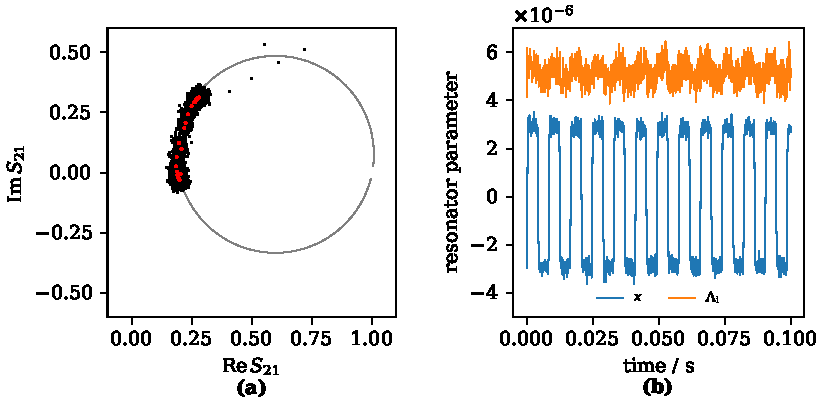
\includegraphics[width=\textwidth]{theory/example_time-ordered_data.pdf}
\caption
[Time-ordered data showing the response to millimeter-wave light.]
{Time-ordered data showing the response to millimeter-wave light.
The device is an aluminum lumped-element KID that was used for the published research described in Chapter~\ref{chp:sensitivity}.
The output of the millimeter-wave source was chopped at \SI{122}{Hz}.
The entire time series is about \SI{4}{s} and is sampled at \SI{31}{kHz}.
\textbf{(a)}
The real and imaginary parts of $\forwardscattering$.
The gray line is the resonator model, the small black points are all the data, and the red points are calculated by averaging all points separated by one period of the signal used to chop the source.
The few points that are widely separated from the rest, to the upper right, were probably caused by a cosmic ray impact.
\textbf{(b)}
The time-varying resonator parameters versus time.
Only \SI{0.1}{s} of data is shown.
The detuning response is much larger than the loss response, as expected for a device with such a low resonance frequency.
}
\label{fig:example_time-ordered_data}
\end{figure}


\chapter{Sources of loss}
\label{chp:loss}

The number of KIDs that can be multiplexed depends on the bandwidth needed by each resonator and the total bandwidth of the readout electronics.
The resonator linewidth -- that is, the full-width, half-maximum bandwidth -- is
$b_\resonator = \loss_\resonator \freadout_\resonator$.
To avoid resonance collisions and minimize electronic crosstalk one might design for adjacent resonance frequencies to be separated by at least 5 times $b_\resonator$.
For reasonable multiplexing, one might require
$\loss_\resonator = \loss_\internal + \loss_\coupling < \num{e-4}$,
corresponding to
$\qf_\resonator > \num{e4}$.
If the resonators are designed so that $\loss_\coupling \approx \loss_\internal$ under the expected optical load, this gives $\loss_\internal \lesssim \num{5e-5}$.
The device sensitivity is improved when the quasiparticle loss dominates the total internal loss so that $\qpfraction$ approaches 1.

The total internal loss is the sum of all the relevant loss terms:
\begin{equation}
\loss_\internal
  =
  \loss_\quasiparticle +
  \loss_\substrate +
  \loss_\tls +
  \loss_\mathrm{nf} +
  \loss_\vortex +
  \cdots,
\end{equation}
where the terms shown here correspond respectively to quasiparticle loss (Section~\ref{sec:theory.response}), loss due to the bulk dielectric substrate and due to two-level systems on nearby surfaces (Section~\ref{sec:loss.dielectrics}), 
loss caused by near-field coupling to normal metal (Section~\ref{sec:loss.near-field}),
and loss due to magnetic flux vortices (Section~\ref{sec:loss.vortex}).
Another possible source of loss is radiation, which may propagate either into the substrate or into free space~\autocite{Sage2011JAP,Zmuidzinas2012ARCMP}.
From the above design requirements, we see that the sum of all non-quasiparticle loss terms should satisfy
$\loss_\internal - \loss_\quasiparticle \ll \num{5e-5}$.


\section{Dielectrics}
\label{sec:loss.dielectrics}

\todo[inline]{Create dielectric constant notation.}
\todo[inline]{Use expressions from Jackson or Pozar to relate the energy stored and lost.}
\todo[inline]{Try to convert the energy storage and loss into a 1D problem.}
\todo[inline]{How are electric and magnetic energies defined when kinetic inductance is significant?}
\todo[inline]{Explain how energy is lost in a bulk dielectric.}
\todo[inline]{Discuss recent TLS papers.}

KIDs are typically fabricated on single-crystal dielectrics with very low loss, such as sapphire and intrinsic silicon.
With careful fabrication and shielding, aluminum co-planar waveguide resonators on sapphire have achieved $\loss_\internal \approx \num{e-6}$ at single-photon readout levels, and as low as $\loss_\internal \approx \num{e-7}$ at higher readout power, which suppresses the dielectric loss~\autocite{Megrant2012APL}.
With one exception, all of the resonators discussed in this thesis are fabricated on high-resistivity, float-zone silicon substrates.
Thus, we can neglect the loss due to the bulk substrate except possibly under dark conditions, where the quasiparticle loss is extremely low.
(The exception to the above is the prototype 23-pixel multichroic KID array discussed in Section~\ref{sec:multichroic.mkidarray02}, which is fabricated on a silicon-on-insulator wafer that contains a silicon oxide layer and a lower-resistivity thick handling wafer.)

Two-level systems (TLS) that occur in amorphous dielectrics at interfaces, such as surface oxides, are a more significant source of loss in superconducting resonators~\autocite{Gao2007APL, OConnell2008APL,Gao2008aAPL,Gao2008bAPL,Wang2009APL,Wenner2011APL}.
The loss due to TLS is given by
\begin{equation}
\loss_\tls
  =
  \loss_{\tls, 0} \frac{\tanh \left( \planck \freadout / \kb \temperature \right)}{\left[1 + (\power_\internal / \power_*)^{\beta / 2} \right]^{1/2}}
\end{equation}
where $\loss_{\tls, 0}$ is the low-power loss, $\power_\internal$ is the power flow into the resonator, $\power_*$ is a critical power that depends on the TLS physics, and the exponent $\beta \approx 1.6 - 2$ depends on the resonator geometry~\autocite{Wang2009APL}.
The critical power is much less than the power levels typically used with KIDs, so we expect
$\loss_\tls \propto \power_\readout^{-0.5}$
or a slightly weaker dependence~\autocite{Zmuidzinas2012ARCMP}.

The loss contributed by dielectrics in a given region depends on the fraction of electric field energy in that region.
Using the definition of the quality factor (or its inverse) we can write
\begin{equation}
\loss_\mathrm{dielectric}
  =
  \sum_i
  \loss_i
  =
  \sum_i
  \alpha_i \tan \delta_i,
\end{equation}
where the index $i$ refers to different dielectrics that occupy different regions, the participation ratio $\alpha_i$ equals the fraction of total electric energy in the volume occupied by the $i$th dielectric, and $\tan \delta_i$ is the intrinsic loss tangent for that dielectric~\autocite{OConnell2008APL}.
Assuming that the losses are small enough not to perturb the field configuration, one can extract the participation ratio for a dielectric using electromagnetic simulations that use several different loss tangents for that dielectric, and fitting the results.

\todo[inline]{TLS fractional frequency shift}


\section{Near-field coupling}
\label{sec:loss.near-field}

\todo[inline]{Discuss radiation into free space: slot antenna.}
\todo[inline]{Discuss radiation into the substrate caused by quasi-TEM phase velocity being faster than in bulk.}

In an early generation of aluminum lumped-element resonators on intrinsic silicon, we measured internal loss $\loss_\internal \approx \num{2.5e-5} = 1 / \num{40000}$, which was significantly lower than expected~\autocite{McCarrick2014RSI}.
At several millimeters on a side, these devices were much larger than the substrate thickness of about \SI{0.5}{mm}.
(This large area was required to produce resonance frequencies around \SI{100}{MHz}.)
These devices were tested in packages machined from oxygen-free, high conductivity copper with gold plating.
The model we developed was that the resonator fields were still sufficiently large at the surface of the package, on the opposite side of the substrate, to produce dissipation due to the interaction with the relatively lossy normal metal.

To test this idea, we fabricated subsequent packages from aluminum alloys (mostly 6061-T6 and QC-10) that we measured to superconduct near the bulk aluminum transition temperature of \SI{1.2}{K}.
Lumped-element resonators tested in these packages had much lower internal loss, typically
$\num{e-6} < \loss_\internal < \num{e-5}$, indicating that switching to aluminum had greatly reduced the dissipation.
Additional evidence for this theory came from later observations that all-niobium lumped element resonators with large capacitors responded to temperature changes well below \SI{1}{K}, qualitatively as expected for aluminum, while co-planar waveguide (CPW) resonators fabricated on the same wafer did not respond to such temperature changes.
This is consistent with the CPW fields being more strongly confined, due to the ground plane, and thus interacting less with the material beyond the substrate. 
\textcite{Goetz2016JAP} showed that this source of loss may also occur in CPW resonators if the substrate is sufficiently thin and the material on the opposite side is sufficiently lossy.

Quantifying the loss in the early experiments was complicated by the fact that the aluminum may have also improved the magnetic shielding around the detectors.
We did not perform additional experiments to conclusively attribute the excess loss to near-field coupling instead of the magnetic flux vortices discussed in the following section.
Superconducting aluminum is expected to have much lower thermal conductivity than copper, due to the absence of an electronic contribution, but we have seen no evidence that the thermal conductivity is insufficient.


\section{Magnetic flux vortices}
\label{sec:loss.vortex}

This section describes an experiment we performed in order to better understand anomalous loss in lumped-element resonators.
This research was published as \fullcite{Flanigan2016bAPL}.

\begin{figure}[tbp]
\centering
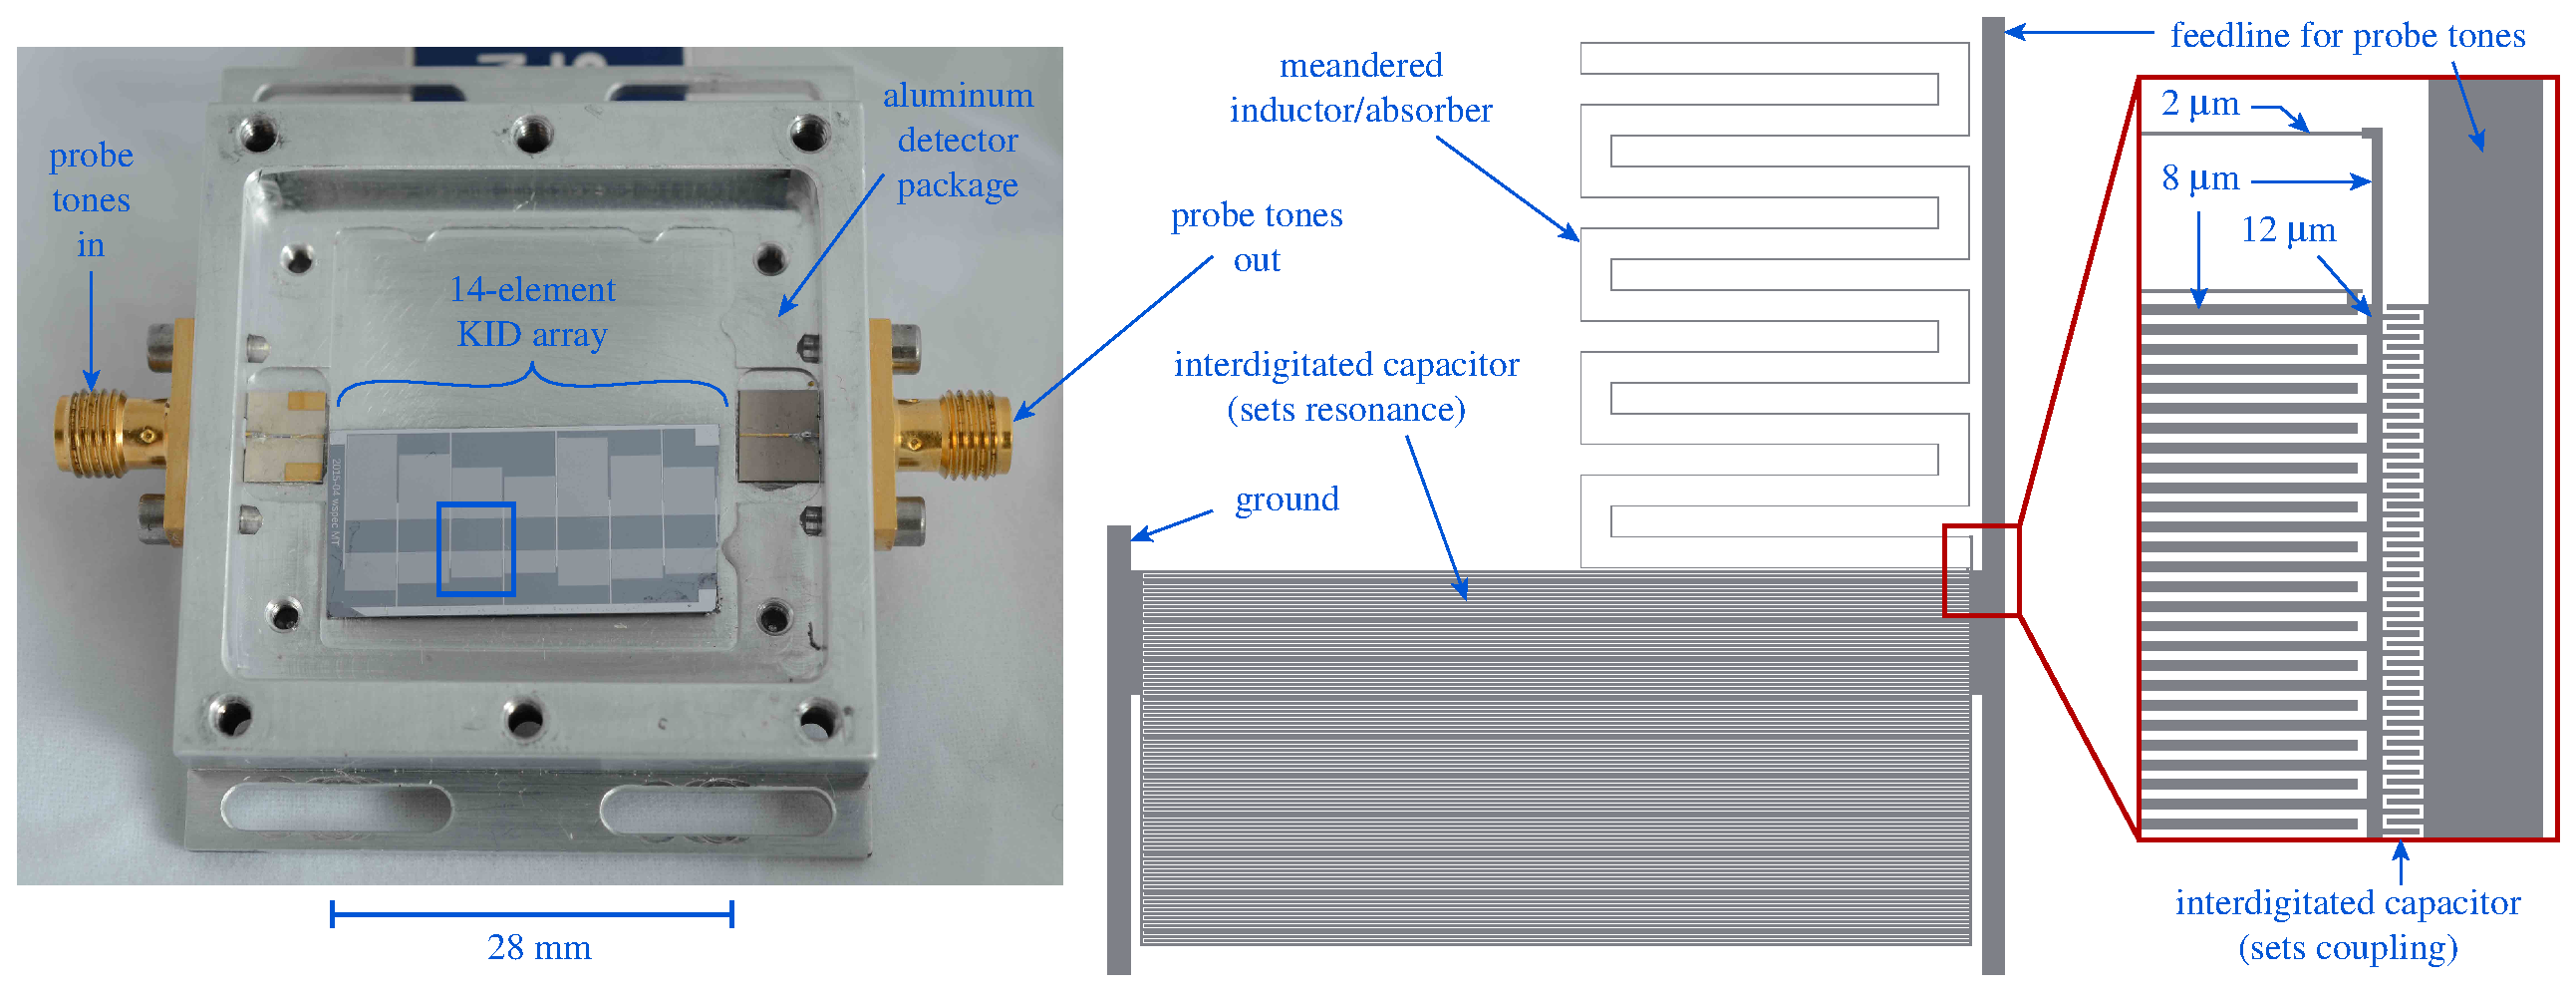
\includegraphics[width=\textwidth]{loss/experiment.eps}
\caption
[Photographs and drawings of the magnetic flux vortex experiment.]
{Photographs and drawings of the magnetic flux vortex experiment.
\textbf{Left:}
A photograph of the detector module tested in this study.
The package lid is removed and the KID array is visible.
Metal clips, not shown here, are used to hold the KID array in place.
\textbf{Center:}
A scale drawing of the lumped-element KID in the blue box on the left.
\textbf{Right:}
Detail of the center panel, showing all of the trace widths used in the resonator.
Our hypothesis is that the ambient magnetic field in the experimental volume was sufficiently strong to create vortices in the widest (\SI{12}{\micro m}) trace, causing unexpectedly high loss.}
\label{fig:loss.experiment}
\end{figure}

\subsection{Introduction}

The suitability of KIDs as a detector technology for photometry depends in part on the fact that they can exhibit high resonator quality factors $\qf_\resonator$.
By tuning each resonator to a unique frequency and taking advantage of the narrow bandwidth corresponding to high $\qf_\resonator$, hundreds or thousands of KIDs may be read out on the same feed line using frequency division multiplexing.
To maintain excellent noise performance and multiplexing capability, it is desirable for the internal loss to be dominated by quasiparticles.

Before incorporating magnetic shielding in the cryostat used to test detectors, we sometimes observed internal quality factors significantly lower than expected.
The packages we use to test KIDs are made from aluminum, a type-I superconductor, which should expel external magnetic fields when superconducting and thus could function as a magnetic shield.
Indeed, after the system is cooled well below the bulk aluminum critical temperature of \SI{1.2}{K}, the KIDs do not detectably respond to externally applied magnetic fields, regardless of their internal quality factors.
However, thin films of type-I superconductors permit magnetic flux entry in the form of vortices~\autocite{Tinkham1963PR,Dolan1974aJLTP}.
These vortices produce loss in thin-film superconducting resonators~\autocite{Song2009PRB,Wang2009APL,Mazin2010APL,Bothner2011APL,Bothner2012PRB,deGraaf2012JAP,Nsanzineza2014PRL,Chiaro2016SUST} because an alternating current in a thin-film trace produces an oscillating Lorentz force on a vortex, and the vortex motion is dissipative~\autocite{Song2009PRB}.

We developed the following hypothesis to explain the excess loss: since the thin film used in the KID has a critical temperature $\tc = \SI{1.4}{K}$, and thus transitions before the package when the system is cooled, vortices formed in the un-shielded film become trapped there and persist when the package becomes superconducting as the system is cooled far below $\tc$.
The presence of vortices at the KID operating temperature (about \SI{150}{mK}) would depend on the field present when the aluminum film transitions.
We tested this hypothesis by varying the strength of the ambient field at \SI{1.4}{K} and measuring $\qf_\internal$ at the KID operating temperature.


\subsection{Experiment}

The resonators used in this study are lumped-element kinetic inductance detectors~\autocite{Doyle2010SPIE} lithographically patterned from a \SI{20}{nm} thick aluminum film on a \SI{500}{\micro m} thick high-resistivity, float-zone silicon substrate.
They were designed for astrophysical measurements at millimeter wavelengths.
The detectors tested in this study were not optically illuminated and were instead mounted inside a light-tight aluminum package with copper tape covering the seam to prevent light leaks.
The package was machined from QC-10, an aluminum alloy for which we have measured a critical temperature near that of bulk aluminum (\SI{1.2}{K}).
The left panel of Figure~\ref{fig:loss.experiment} is a photograph of the KID array in the package.
Fourteen resonators were patterned in this array.
For this study we focused on just three of these resonators, with resonance frequencies $\freadout_\resonator$ of \SIlist{78;116;161}{MHz}.
The center and right panels of Figure~\ref{fig:loss.experiment} are drawings of one resonator that show the various trace widths used in different regions.
The width of the traces is important here because magnetic flux vortices will form at lower field magnitudes in wider traces.
Figure~\ref{fig:starcryo_cryostat_with_optics_box} is a photograph of the cryostat used in this experiment.
Inside the cryostat, the package was mounted to a gold-plated copper plate that is thermally connected to the cold stage of an adiabatic demagnetization refrigerator (ADR) backed by a helium pulse tube cooler.

The ambient magnetic field of the room in the region of the package was measured to be downward to within \SI{10}{\degree} of vertical.
We do not consider any effect of the in-plane component of the magnetic field and refer hereafter to only the vertical component of the field, which is normal to the aluminum film.
All reported fields were measured using a gaussmeter (Lake Shore model 425) that uses a calibrated single-axis Hall probe (Lake Shore model HMMA-2504-VR).
Taking the upward direction to be positive, the ambient field is $\bfield_\ambient = -30 \pm 1 \, \si{\micro T}$.
While collecting data over several weeks we frequently measured the ambient field near the cryostat, and observed changes within a range of a few \si{\micro T}.
Since these variations are small compared to the range of applied fields, we did not attempt to correct for them.

\begin{figure}[htb]
\centering
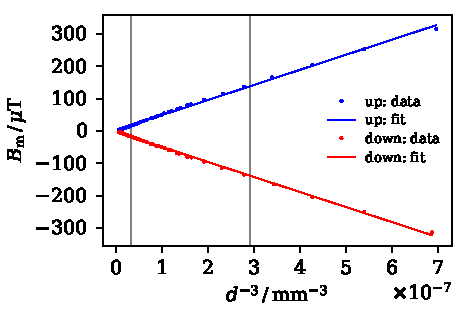
\includegraphics[width=0.75\textwidth]{loss/magnet_array_field_vs_distance.pdf}
\caption[The measured magnetic field of the magnet array versus distance along its center axis.]
{The measured magnetic field of the magnet array versus distance along its center axis.
The fit is acceptable over the range of distances used in the experiment, shown by the vertical gray lines.
The labels refer to the orientation of the field produced by the array.}
\label{fig:magnet_array_field_vs_distance}
\end{figure}

We created a magnetic field normal to the KIDs using an array of seven small NdFeB permanent magnets mounted outside the cryostat.
The magnets were arranged in a triangular lattice \SI{70}{mm} in diameter in order to produce an approximately uniform field at the detector array, which is \SI{28}{mm} by \SI{13}{mm}.
The lateral variation in the field was measured to be less than 10\%. 
As shown in Figure~\ref{fig:magnet_array_field_vs_distance}, the normal component of the magnet array field $\bfield_\magnetarray(\distance)$ was measured as a function of distance $\distance$ from the plane of the magnets along the center axis.
In both orientations, the data were fit to the model
\begin{equation}
\bfield_\magnetarray(\distance)
  =
  a \distance^{-3} + b,
\label{eqn:magnet_array_field_vs_distance}
\end{equation}
as expected for the on-axis field of a dipole plus a possible offset.
The offsets resulting from the fits are a few \si{\micro T}.

To record a data set, we first establish a magnetic field configuration by positioning the magnet array some chosen distance from the KID array.
The cryostat shells are aluminum (well above its $\tc$), the cold stage plate is gold-plated copper, and the other materials near the package are non-magnetic, except where noted below.
Thus, the ambient magnetic field and the field from the permanent magnets should enter the cryostat unaltered.
The total magnetic field that we calculate is
$\bfield(\distance) = \bfield_\ambient + \bfield_\magnetarray(\distance)$,
using the fits of Equation~\ref{eqn:magnet_array_field_vs_distance}.
After setting the field, we cycle the ADR, let the package and KID array cool well below $\tc$, regulate the temperature of the package at $153 \pm \SI{4}{mK}$, then collect data.
For each resonator we first, using a ROACH-based readout, sweep the readout tone frequency across the resonance and fit the data to the resonator model in Equation~\ref{eqn:forwardscattering}, then set the readout tone to the resonance frequency obtained from the fit and collect time-ordered data for \SI{30}{s}.
The data set yields a value for $\qf_\internal$ and a noise spectrum for that magnetic field configuration.
All measurements were recorded using a constant readout tone power of approximately \SI{-100}{dBm} on the feedline, below the onset of nonlinear effects in the resonators.
This process was repeated for a range of distances.
For comparison, we also recorded data with a five-sided mu-metal shield surrounding the cryostat.
The contribution of the ambient field to the interior of the mu-metal shield was measured to be less than \SI{1}{\micro T}, and we take it to be zero when the shield is used.

\subsection{Results}

\begin{figure}[tbp]
\centering
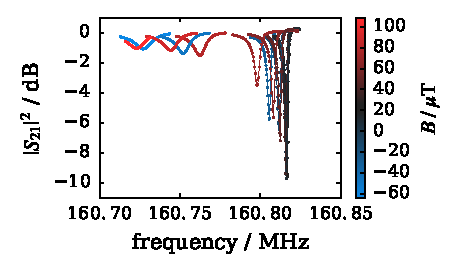
\includegraphics[width=0.75\textwidth]{loss/s21_vs_f_colorbar_B.eps}
\caption
[Forward scattering parameter data at different magnetic fields.]
{The points are forward scattering parameter $\forwardscattering$ data from sweeps of the readout tone across the \SI{161}{MHz} resonance.
The data have been normalized to 1 off-resonance using the fits to the resonator model, which are plotted as lines.
The color bar shows the calculated field $\bfield$ in which the resonator was cooled.}
\label{fig:loss.s21_vs_f}
\end{figure}

Figure~\ref{fig:loss.s21_vs_f} shows the behavior of one resonator as $\bfield_\magnetarray$ is varied.
At higher field magnitudes, $\freadout_\resonator$ and $\qf_\internal$ both decrease, while $\qf_\coupling$ does not change.
As shown in Figure~\ref{fig:loss.iQi_vs_B}, the loss minimum for all three resonators occurs over a range of fields centered near $\bfield = 0$, and the loss increases as the field magnitude departs from this central value.
This result is consistent with previous studies of vortices in thin films, which have generally found that increasing field magnitude creates both higher vortex density in narrow strips and higher loss in resonators.
Direct imaging of the field near narrow strips of thin-film niobium~\autocite{Stan2004PRL} and YBCO~\autocite{Kuit2008PRB} has shown that few or no vortices enter the strip below a threshold field magnitude $\bfield_\threshold$, which varies with the trace width $\tracewidth$ approximately as
$\bfield_\threshold \sim \fluxquantum \tracewidth^{-2}$,
where $\fluxquantum$ is the flux quantum.
Measurements of the vortex-induced loss in aluminum and rhenium thin-film resonators cooled in a magnetic field normal to the film showed that the field had no effect on the loss below a threshold magnitude, and that well above this level the loss was approximately proportional to the excess magnitude above the threshold~\autocite{Song2009PRB}.
The entry of even a single vortex into a region of high current flow in a resonator can cause significant loss~\autocite{Nsanzineza2014PRL}.

\begin{figure}[tb]
\centering
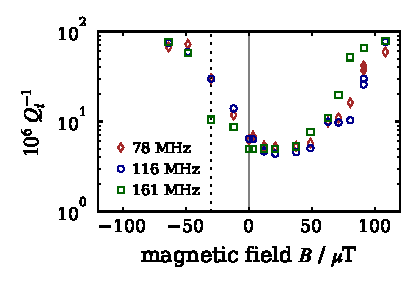
\includegraphics[width=0.7\textwidth]{loss/iQi_vs_B.eps}
\caption
[The inverse internal quality factor of three resonators versus magnetic field.]
{The inverse internal quality factor versus magnetic field ($\bfield_\ambient + \bfield_\magnetarray$), plotted for three resonators.
The vertical gray line marks the field condition when a mu-metal magnetic shield is placed around the cryostat and no magnet array is applied.
The dotted black line marks the field condition with no magnetic shield present and no magnet array.
The points to the left of the dotted black line were recorded with the magnet array polarity reversed so that it augmented the ambient field.
The minimum is likely shifted away from zero because the Heli-Coil inserts in the cold plate of the cryostat can produce a field of about $\SI{25}{\micro T}$.}
\label{fig:loss.iQi_vs_B}
\end{figure}

In Figure~\ref{fig:loss.iQi_vs_B}, the center of the low-loss region is offset from zero by about \SI{25}{\micro T}.
We believe that this offset is caused by fields not included in the calculation of $\bfield$.
First, during the course of these measurements we discovered that the stainless steel Heli-Coil inserts in the millikelvin stage plate are magnetized.
While this Heli-Coil field is not constant across the KID array, its magnitude and direction approximately account for the observed offset.
Second, while the ADR is well-shielded with Vanadium Permendur, it produces a strong field and some leakage is possible.
To estimate the stray field from the ADR, we conducted a separate measurement of the vertical component of the field $\bfield_\ambient + \bfield_\adr$.
Because our Hall probe cannot operate at cryogenic temperatures we made the field measurement \SI{6}{cm} below the package just outside the cryostat.
\todo[inline]{What was the peak field due to the ADR?}
When the current through the ADR magnet is at its peak and the package is at \SI{3}{K}, the ADR field is detectable. % $\bfield_\adr \approx ?$.
However, $\bfield_\adr$ decreases during the ADR cycle because the current in the coil decreases, and the measured field returns to within the measurement uncertainty of $\bfield_\ambient$ when the package reaches \SI{1.4}{K}, indicating that $\bfield_\adr$ is small at the relevant point in the cycle.
Our conclusion is that the ADR field could produce a shift in the center of the low-loss region shown in Figure~\ref{fig:loss.iQi_vs_B}, but it is likely to be a smaller source of systematic error than field from the Heli-Coil inserts.

Interpreting the offset in this way, the threshold field for vortex entry is $\bfield_\threshold \approx \SI{30}{\micro T}$.
As shown in Figure~\ref{fig:loss.experiment}, the widest traces in these resonators are \SI{12}{\micro m}; these are located only where the coupling capacitor runs along part of the much larger capacitor that sets the resonance frequency.
The threshold field for this width is expected to be $\fluxquantum \tracewidth^{-2} = \SI{14}{\micro T}$ (up to a factor that is theoretically expected to be of order unity).
Since these wider traces are near the junction with the inductor, most of the current will flow through them on the way into the \SI{8}{\micro m} wide interdigital capacitor tines, so we expect vortex entry here to produce loss.
Previous measurements of similar lumped-element resonators with a maximum trace width of \SI{8}{\micro m} consistently exhibited high $\qf_\internal$~\autocite{McCarrick2014RSI}.
The crucial difference seems to be that the \SI{12}{\micro m} trace in these devices permits vortex entry at a threshold field less than the ambient field, while the \SI{8}{\micro m} traces did not.

\begin{figure}[tb]
\centering
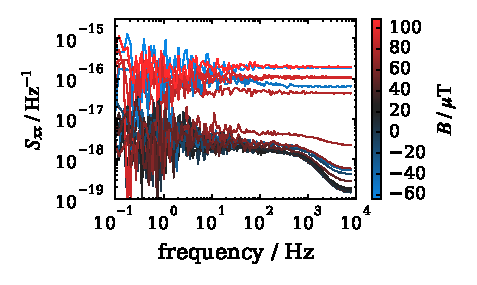
\includegraphics[width=0.75\textwidth]{loss/Sxx_vs_f_colorbar_B.eps}
\caption
[The spectral density of the fractional frequency detuning time series data from one resonator at different magnetic fields.]
{The spectral density of the fractional frequency detuning time series data from the \SI{161}{MHz} resonator.
The color scale corresponds to the magnetic field ($\bfield_\ambient + \bfield_\magnetarray$).
To more clearly show the trend at low frequencies, the lowest 15 harmonics of the \SI{1.412}{Hz} pulse tube cooler frequency have been masked in all of the spectra.
The color bar is the same as Figure~\ref{fig:loss.s21_vs_f}.
}
\label{fig:loss.Sxx_vs_f}
\end{figure}

In SQUIDs, the presence of vortices is known to produce flux noise with a typical $1 / f$ spectral density~\autocite{Dantsker1997APL}.
To investigate the possibility of vortices producing excess noise in the resonators, we decomposed the on-resonance time-ordered data into two real time series corresponding to the fractional frequency shift $\detuning(\time)$ and inverse internal quality factor, or internal loss, $\qf_\internal^{-1}(t)$.
The spectral density $\spectraldensity_{\detuning\detuning}(\faudio)$ of the $\detuning(\time)$ data is shown in Figure~\ref{fig:loss.Sxx_vs_f}.
Larger field magnitudes correspond to higher loss, and thus a higher amplifier noise level.
Besides this expected effect of lower $\qf_\internal$, we see no evidence for additional contributions to the noise due to the presence of vortices.
Only amplifier noise is visible in the internal loss fluctuation spectra (not shown here).

To verify that the superconducting detector package is an effective magnetic shield when cold, we altered the magnetic field after the package had fully cooled and looked for changes in $\qf_\internal$ and $\freadout_\resonator$.
We cooled the package in an initial field condition near the center of the low-loss region in Figure~\ref{fig:loss.iQi_vs_B}, collected the nominal data set, moved the magnet array to establish a new high-field condition at the package, and then collected a second data set.
Between these data sets, neither $\qf_\internal$ nor $\freadout_\resonator$ changed significantly, indicating that the perturbation in the applied magnetic field condition did not affect the resonators either through vortex entry or kinetic inductance non-linearity~\autocite{Healey2008APL,Zmuidzinas2012ARCMP}.
Note that these second points are not shown in Figure~\ref{fig:loss.iQi_vs_B}.
The observation that some vortices remain in the film even when the package is shielding the resonators is consistent with the hysteretic magnetization curves observed in field-cooled type-I thin films~\autocite{Chang1963PL,Miller1964RMP} and with hysteretic loss observed in niobium thin-film resonators~\autocite{Bothner2012PRB}.
We can use a result of \textcite{Stan2004PRL} to estimate the number of vortices $\vortexnumber$ present just below $\tc$ in a trace of width $\tracewidth = \SI{12}{\micro m}$ and length $\tracelength = \SI{1000}{\micro m}$ (this length varies substantially between resonators):
$\vortexnumber
  \approx
  (\bfield - \bfield_\threshold) \tracewidth \tracelength / \fluxquantum
  \sim
  300$
at the highest field magnitudes.

\subsection{Discussion}

When the system is at the operating temperature, the superconducting aluminum package provides some magnetic shielding.
This could be useful for detectors deployed on a telescope, which may be required to move through the Earth's field.
However, our results show that additional shielding is necessary to prevent vortex creation when the module passes through the superconducting transition.
A detector package made from a type-I superconductor with a $\tc$ higher than that of the film should be more effective.

The mu-metal magnetic shield surrounding the cryostat greatly attenuates external fields, but hardware elements such as Heli-Coil inserts or nickel-plated connectors, which are commonly used near the detector package inside the cryostat, could produce magnetic fields strong enough to yield vortices~\autocite{Wang2009APL,Chiaro2016SUST}.

The devices themselves may be modified to reduce vortex formation by adding flux-trapping holes~\autocite{Bothner2011APL,Chiaro2016SUST} or by using a fractal geometry~\autocite{deGraaf2012JAP}.
To cancel the ambient field, it may be more convenient to use a Helmholtz coil instead of permanent magnets~\autocite{Song2009PRB,Mazin2010APL,Bothner2012PRB,Nsanzineza2014PRL}.
Finally, heating the KID arrays inside the superconducting package to the point where the aluminum film becomes normal would cause the vortices to dissipate, and they should not reappear if the package remains superconducting during this process.

\chapter{Sensitivity and noise}
\label{chp:sensitivity}

As discussed in Section~\ref{sec:cmb.experiment.signals}, detectors that measure the CMB must make high-sensitivity measurements of faint signals at low audio frequencies.
The sensitivity of photometric detectors like those discussed in this thesis is a question of signal-to-noise: for a given measurement time, what is the ratio of detected power to the standard deviation of the mean of this power?
This ratio determines how long it takes to measure a given fractional anisotropy at some point on the sky.
In this chapter, I use the responsivity equations derived in Section~\ref{sec:theory.response} to compare the relevant noise sources and illustrate their variation with variables such as optical load, detector temperature, and readout power.

In Section~\ref{sec:sensitivity.photon_noise}, I discuss the generation noise due the randomness of photon arrival, which is the dominant noise source for an ideal photometric detector.
In Section~\ref{sec:sensitivity.quasiparticle}, I discuss the fundamental noise due to random generation and recombination of quasiparticles, using the quasiparticle number model introduced in Chapter~\ref{chp:theory}.
In Section~\ref{sec:sensitivity.tls}, I discuss noise due to two-level systems (TLSs) in dielectrics on interfaces near a resonator, which cause fluctuations in the dielectric constant and thus frequency noise.
In Section~\ref{sec:sensitivity.readout}, I discuss noise caused by the electronics used to read out the detectors, especially the cryogenic amplifier.
Finally, Section~\ref{sec:sensitivity.measuring} contains published research describing measurements of photon noise in a lumped-element KID.


\section{Photon noise and noise-equivalent power}
\label{sec:sensitivity.photon_noise}

A hypothetical noiseless detector that measures a light source with a constant brightness will still measure fluctuations due to the randomness of photon arrival times.
This photon noise is the fundamental noise source for photometry.
Consider a detector for photons with frequency $\foptical$ that occupy some effective optical bandwidth
$\opticalbandwidth \ll \foptical$.
The occupancy of the photon state is $\photonoccupancy$ and the band-average detection efficiency is $\efficiency$.
Then, the average detection rate, which equals the probability per unit time for photon detection, is
\begin{equation}
\eventrate
  =
  \efficiency \photonoccupancy \opticalbandwidth.
\end{equation}
Measuring this average photon arrival rate (or, equivalently, the power) is the goal of photometry.
The variance of the mean of the detected photon rate after detection time $\detectiontime$ is~\autocite{Zmuidzinas2003ApplOpt}
\begin{equation}
\sigma_\eventrate^2
  =
  \detectiontime^{-1} \opticalbandwidth \efficiency \photonoccupancy (1 + \efficiency \photonoccupancy)
  =
  \detectiontime^{-1} \left( \eventrate + \eventrate^2 / \opticalbandwidth \right).
\label{eqn:variance_mean_eventrate}
\end{equation}
The first term here is due to photon quantization and is called the shot noise.
The second term is due to correlations between photon arrival times due to the Bose statistics of the photons, and it is called the wave noise or photon-bunching noise.
(The variance of the thermal occupancy of a photon mode is $\sigma_\photonoccupancy^2 = \photonoccupancy + \photonoccupancy^2$.)
Despite this connection to particle statistics, the wave noise term actually describes the classical noise level, as it dominates at high power.
It can be thought of as being due to beating between nearby Fourier components of a classical signal that occupies the bandwidth $\opticalbandwidth$.
More accurate formalisms for calculating the photon noise involve integrals over the optical band~\autocite{Zmuidzinas2003ApplOpt}.
Going beyond the narrowband approximation requires knowledge of the absorption spectrum, so $\opticalbandwidth$ as used here is an effective bandwidth.

If photon noise is the only noise source, then the signal-to-noise ratio is
\begin{equation}
\frac{\eventrate}{\sigma_\eventrate}
  =
  \left(
  \frac{\detectiontime \opticalbandwidth}
  {1 + (\efficiency \photonoccupancy)^{-1}}
  \right)^{1/2}.
\end{equation}
When $\efficiency \photonoccupancy \ll 1$ increasing $\efficiency$ increases the signal-to-noise, but when $\efficiency \photonoccupancy \gg 1$, the signal-to-noise is independent of the efficiency.

The signal-to-noise ratio increases with increasing optical bandwidth, but CMB experiments are generally not able to improve their sensitivity in this way.
For CMB measurements from the ground, the observation bands are constrained to lie between strong atmospheric emission lines.
Even for satellite missions that do not see the atmosphere, there is still a tension between increasing $\opticalbandwidth$ and obtaining independent measurements of the sky at different frequencies, in order to characterize Galactic foregrounds.

We can convert the variance of the mean of the detected photon flux into the variance of the mean of the detected power using
$\pdv*{\power}{\eventrate} = \planck \foptical$:
\begin{equation}
\sigma_\power^2
  =
  \detectiontime^{-1} (\planck \foptical \power + \power^2 / \opticalbandwidth).
\end{equation}
A common figure of merit for the sensitivity of a photometric detector is the noise-equivalent power (NEP), defined to be the standard error of the mean in the inferred optical power at a given point in the optical system after
$\detectiontime = \SI{0.5}{s}$ of averaging.
Inserting this value in the above equation gives
\begin{equation}
\nep_\photon^2
  =
  2 \planck \foptical \power + 2 \power^2 / \opticalbandwidth.
\end{equation}

For the measurements presented later in this chapter, we must relate the NEP to the spectral density $\spectraldensity_{\power \power}$, which can be estimated as the Fourier transform of the time-ordered data in units of power.
When discussing detector noise data I use \textit{spectral density} to mean the single-sided power spectral density.
That is, the integral of the spectral density over positive frequencies is the variance of the mean.
Using Parseval's theorem, one can show that
$\nep^2 = (\pdv*{x}{\power})^{-2} \detectorwhite^2 $,
where $x$ is the quantity that the detector measures and $\detectorwhite^2$ is the white component of the spectral density of $x(\time)$.
In Section~\ref{sec:sensitivity.measuring}, I will present measurements of NEP obtained by measuring the white component of the detector noise.

The NEP is a measure of random error at a particular location in the system.
Consider two locations in an optical system, labeled A and B, with A downstream of B.
The optical power $\power$ at these locations is related by
$\power_\mathrm{A} = \efficiency_\mathrm{B} \power_\mathrm{B}$
with $\efficiency_\mathrm{B} \le 1$.
Then, given the variance of the mean of $\power_\mathrm{A}$, the variance of the mean of $\power_\mathrm{B}$ is larger by a factor of $\efficiency_\mathrm{B}^{-2}$.
When the reference point is the power absorbed in a detector, the corresponding NEP is sometimes called an \textit{electrical} NEP.
The NEP referenced to a source plane is sometimes called an \textit{optical} NEP.

\begin{comment}
Some authors define a frequency-dependent $\nep^2(\faudio)$ to be the value at frequency $\faudio$ of the single-sided auto-spectral density of the time-ordered data in units of the optical power at some reference location.
Clearly, if the noise is white, this definition is equivalent to that used here.
\end{comment}

\section{Quasiparticle generation and recombination noise}
\label{sec:sensitivity.quasiparticle}

In the quasiparticle number model discussed in Chapter~\ref{chp:theory}, the response of a detector is proportional to the number of excitations.
Fluctuations in this number are the fundamental source of noise.
In this chapter I use results from Section~\ref{sec:theory.qpnumber} along with a simple model for shot noise to derive results for the spectrum of the fluctuations in the quasiparticle number.
I consider the same generation sources discussed in Section~\ref{sec:theory.quasiparticle.generation}, namely, phonons entering from the substrate, optical photons, and readout photons.

Consider a situation in which the quasiparticle number fluctuates about a steady-state value, so that the total average decay rate equals the total average generation rate:
\begin{equation}
\qprecombinationeff \ssqpnumber^2 / \volume + \qpsingledecay \ssqpnumber
  =
  \ssRate_\qprecombinationeff + \ssRate_\qpsingledecay
  =
  \ssRate_\generation,
\end{equation}
where $\ssRate_\generation$ is the total average generation rate, and all rates are defined to be positive.
Each process has a corresponding \textit{shot size}, which is the number of quasiparticles that are created or annihilated in each event.
I take the shot size for thermal generation to be 2, since the devices are operated at temperature $\temperature \ll 2 \gap / \kb$ and thus phonons with enough energy to break multiple Cooper pairs should be rare.
The average number of quasiparticles $\qpperphoton \ge 2$ generated by an optical photon depends on the ratio of the photon and gap energies, as discussed in Section~\ref{sec:theory.response.photodetection}.
I assume that the shot size is also 2 for pair-breaking by readout photons.
Finally, quasiparticles may tunnel individually into a superconductor from another metal, with a shot size of 1.
For the formation of a single Cooper pair through recombination with phonon emission the shot size is again 2, while it is 1 for all of the single-quasiparticle decay processes discussed in Section~\ref{sec:theory.quasiparticle.single_decay}.

For the remainder of this chapter I will assume that the single-quasiparticle processes are negligible, which seems to be the case in our devices except, possibly, when they are tested dark.
(See Section~\ref{sec:theory.qpnumber.qprelaxationtime}.) 
With this assumption, all of the relevant processes except possibly optical generation have a shot size of 2.
For aluminum films illuminated by \SI{150}{GHz} radiation this shot size is 2 as well.

Consider a current $\current = \quantum \eventrate$ consisting of flow events that occur at an average rate $\eventrate$, where each event corresponds to the flow of $\quantum$ particles.
Assume that the current $\current$ is stationary and that the events are uncorrelated.
(From this point on I will not write the over-bars, since all of the rates here are steady-state rates.)
Then, for positive frequencies the single-sided spectral density of the current equals the Poisson value
\begin{equation}
\spectraldensity_{\current \current}
  =
  2 \quantum \current = 2 \quantum^2 \eventrate,
\end{equation}
with units of current squared per hertz.
For example, the familiar expression for the single-sided spectral density of fluctuations in an electric current is
\begin{equation}
\spectraldensity_{\current \current}
  =
  2 \unitcharge \current
  =
  2 \unitcharge^2 \eventrate,
\end{equation}
where $\unitcharge$ is the unit charge.
There are corrections to this simple expression that depend on the statistics of the particles involved~\autocite{Blanter2000PR}, but we can ignore these except where noted.

Returning to the case of quasiparticle generation and decay, the current in this case is $\Rate$, the shot size $\quantum$ depends on the process, and the event rate is $\eventrate = \Rate / \quantum$.
The spectral density of the quasiparticle recombination rate, for which the shot size is 2, is
\begin{equation}
\spectraldensity_{\Rate_\recombination \Rate_\recombination}
  =
  2 \cdot 2 \cdot \Rate_\recombination.
  =
  4 \Rate_\recombination.
\end{equation}
The results for thermal generation and readout generation, which also have a shot size of 2, are very similar:
\begin{align}
\spectraldensity_{\Rate_\thermal \Rate_\thermal}
  &=
  4 \Rate_\thermal; \\
\spectraldensity_{\Rate_\readout \Rate_\readout}
  &=
  4 \Rate_\readout.
\end{align}
Using a result from the previous section, for optically-excited quasiparticles generated at a rate $\Rate_\optical$ with shot size $\qpperphoton$, the spectral density is
\begin{equation}
\spectraldensity_{\Rate_\optical \Rate_\optical}
  =
  2 \qpperphoton \Rate_\optical + 2 \Rate_\optical^2 / \opticalbandwidth.
\label{eqn:spectraldensity_generation_photon}
\end{equation}
The first term is the expected shot noise term, while the second term appears because the photon arrival times are correlated.
An ideal detector would add a noise level less than this photon noise contribution, which is the fundamental lower limit for the measurement noise.

These generation and decay processes are uncorrelated, so the spectral density of the detector noise is given by their sum.
The response of a KID is proportional to the number of quasiparticles, not the generation rate, and the spectral densities of these are related by the square of $\pdv*{\qpnumber}{\Rate_\generation} = \qprelaxationtime$.
The spectral density of the quasiparticle number is
\begin{equation}
\spectraldensity_{\qpnumber \qpnumber}
  =
  \qprelaxationtime^2
  \left(
  2 \qpperphoton \Rate_\optical + 2 \Rate_\optical^2 / \opticalbandwidth
  + 4 \Rate_\thermal + 4 \Rate_\readout + 4 \Rate_\recombination \right).
\label{eqn:spectraldensity_qpnumber}
\end{equation}
To make contact with other work, consider the equilibrium state, in which only thermal generation and pair recombination occur.
Then, 
$\Rate_\recombination = \Rate_\generation = \Rate_\thermal$,
and
\begin{equation}
\spectraldensity_{\qpnumber \qpnumber}
  =
  8 \qprelaxationtime^2 \Rate_\generation
  =
  4 \qprelaxationtime \qpnumber,
\end{equation}
where we used
$\qpnumber = 2 \Rate_\generation \qprelaxationtime$ from
Equation~\ref{eqn:qpnumber.responsivity} with $\qpsingledecay = 0$.
Recall the result of Section~\ref{sec:theory.qpnumber} that fluctuations in the quasiparticle system are rolled off at a frequency
$\faudio_\quasiparticle = (2 \pi \qprelaxationtime)^{-1}$.
If we insert this frequency dependence by hand, we obtain
\begin{equation}
\spectraldensity_{\qpnumber \qpnumber}(\faudio)
  =
  \frac{4 \qprelaxationtime \qpnumber}{1 + (2 \pi \faudio \qprelaxationtime)^2}.
\end{equation}
This matches the result given by \textcite{Wilson2004PRB}, who derived this equation and compared it to measurements of quasiparticle number fluctuations in thermal equilibrium.

The steady-state generation and recombination rates must balance:
$\Rate_\recombination
  =
  \Rate_\generation
  = 
  \Rate_\optical + \Rate_\thermal + \Rate_\readout$,
so each generation process has a corresponding recombination contribution.
There is noise associated with energy entering the detector, and there is additional noise associated with this energy leaving it.
In the thermal equilibrium case, the two noise contributions are necessarily equal because the shot sizes are the same.

We can obtain additional insight by writing everything in terms of the generation rates.
Using
$\qprelaxationtime^2 = (4 \qprecombinationeff \Rate_\generation / \volume)^{-1}$, again from Equation~\ref{eqn:qpnumber.responsivity} (still ignoring single-quasiparticle generation and decay), results in
\begin{align}
\begin{split}
\spectraldensity_{\qpnumber \qpnumber}
  &=
  \frac
  {(2 \qpperphoton + 4) \Rate_\optical + 2 \Rate_\optical^2 / \opticalbandwidth
  + 8 \Rate_\thermal + 8 \Rate_\readout}
  {4 \qprecombinationeff \Rate_\generation / \volume} \\
  &=
  \frac{\volume}{\qprecombinationeff}
  \frac{(\qpperphoton / 2 + 1) \Rate_\optical + \Rate_\optical^2 / 2 \opticalbandwidth
  + 2 \Rate_\thermal + 2 \Rate_\readout}
  {\Rate_\optical + \Rate_\thermal + \Rate_\readout}.
\end{split}
\label{eqn:spectraldensity_qpnumber_generation}
\end{align}
If optical generation dominates, which is the ideal case, this reduces to
\begin{equation}
\spectraldensity_{\qpnumber \qpnumber}
  =
  \frac{\volume}{\qprecombinationeff}
  \left( \qpperphoton / 2 + 1 + \frac{\Rate_\optical}{2 \opticalbandwidth} \right).
\label{eqn:spectraldensity_qpnumber_optical}
\end{equation}
If the wave noise term is negligible or not present, then the quasiparticle noise is constant.
This surprising prediction is observed in the data presented in Section~\ref{sec:sensitivity.measuring}.
Figure~\ref{fig:measuring.results}(a) shows fractional frequency noise spectra taken with varying illumination levels from a coherent source, for which the photon arrival times are uncorrelated and the wave noise term is absent.
Table~\ref{tab:cwfitparams} gives the parameters extracted from the fits.
The detuning spectral density $\spectraldensity_{\detuning \detuning}$ is proportional to the quasiparticle number spectral density.
The white component of $\spectraldensity_{\detuning \detuning}$ varies only by a factor of two, while the generation rate varies by a factor of
$\SI{29}{pW} / \SI{0.08}{pW} \sim 400$.
In contrast, the white component of the fractional frequency noise spectra shown in Figure~\ref{fig:measuring.results}(b) and summarized in Table~\ref{tab:bbfitparams} does increase with increasing chaotic illumination, due to the wave noise.

Ignoring the wave noise term, the ratio of the photon noise to the recombination noise is $\qpperphoton / 2 \ge 1$.
Thus, the total recombination noise may be negligible when $\qpperphoton \gg 2$, but not when $\qpperphoton \gtrsim 2$, as in this work.
There may be an advantage to using materials with a smaller gap energy to increase $\qpperphoton$, if the detectors can still be cooled sufficiently to keep thermal generation negligible.

Finally, we can relate the quasiparticle recombination noise to NEP, referenced to incident power, using
$\pdv*{\power_\incident}{\Rate_\generation} = \planck \foptical / \efficiency_\incident \qpperphoton$:
\begin{equation}
\nep^2_{\incident, \recombination}
  =
  \left( \frac{\planck \foptical}{\efficiency_\incident \qpperphoton} \right)^2 \spectraldensity_{\Rate_\recombination \Rate_\recombination}.
\end{equation}
If optical generation dominates, so that $\Rate_\recombination = \Rate_\generation = \Rate_\optical$, then we can express this in terms of the incident power:
\begin{equation}
\nep^2_{\incident, \recombination}
  =
  \left( \frac{\planck \foptical}{\efficiency_\incident \qpperphoton} \right)^2 4 \Rate_\optical
  =
  \frac{2}{\qpperphoton} \frac{2 \planck \foptical \power_\incident}{\efficiency_\incident}
  =
  \frac{4 \gap_\zerotemp \power_\incident}{\pbefficiency \efficiency_\incident},
\end{equation}
where we absorbed one factor of $\efficiency_\incident$ into $\power_\incident = \power_\optical / \efficiency_\incident$.
In the middle expression, we again see that the ratio of the photon shot noise to the recombination noise equals $\qpperphoton / 2$.
An expression for recombination noise that equals half the latter expression above has appeared in the literature~\autocite{Yates2011APL,Janssen2013APL,deVisser2014NatComm,Hubmayr2015APL,McCarrick2014RSI}.
Because we use this equation as part of the NEP model in the measurements discussed in Section~\ref{sec:sensitivity.measuring}, we are unable to empirically demonstrate here that the equation given here is correct.

\section{Two-level system noise}
\label{sec:sensitivity.tls}

\todo[inline]{Flesh out TLS noise: physical model, latest papers, etc.}
The noise sources discussed above are fundamental to KID detection and measurement.
An important non-ideal noise source is the two-level systems that were discussed in Section~\ref{sec:loss.dielectrics} in terms of the loss they produce.
These TLS have an electric dipole moment and thus may affect the local dielectric constant.
Fluctuations in the dielectric constant near the resonator affect the resonance frequency, and thus TLS noise is most usefully expressed in terms of a detuning spectral density
$\spectraldensity_\tls \equiv \spectraldensity_{\detuning \detuning, \tls}$.
The TLS spectral density is found to obey
\begin{equation*}
\spectraldensity_\tls(\faudio, \power_\internal)
  \propto
  \faudio^{-1/2} (1 + \power_\internal / \power_*)^{-1/2},
\label{eqn:spectraldensity_tls}
\end{equation*}
where, as in Section~\ref{sec:loss.dielectrics}, $\power_\internal$ is the internal readout power and the critical power $\power_*$ is small compared to the readout power levels typically used with KIDs~\autocite{Gao2007APL,Gao2008bAPL,Barends2010APL,Zmuidzinas2012ARCMP,Neill2013APL}.
The TLS noise may thus be reduced by increasing the readout power.
As the power increases, the resonance will eventually bifurcate.
The maximum readout power that can be used depends on how deep into this regime it is possible to operate the detector.
Measurements in this state are more difficult to interpret, and the laboratory measurements shown here are obtained with the readout power below the bifurcation level, to ensure that the linear resonator model fits well.

One unfortunate property of TLS noise is that its spectral density in units of generation rate or NEP actually increases with absorbed power.
The reason for this is that a factor of $\qprelaxationtime$ appears in the derivative
$\pdv*{\detuning}{\power_\optical}$,
so
\begin{equation}
\nep_\tls^2
  =
  \spectraldensity_\tls
  \left( \pdv{\detuning}{\power_\optical} \right)^{-2}
  \propto
  \qprelaxationtime^{-2} \spectraldensity_\tls
  \propto
  \power_\optical \spectraldensity_{\detuning \detuning}.
\end{equation}
Thus, unless the internal power is increased, the squared NEP due to TLS will increase linearly with absorbed power, like the shot noise.
This fact is important for the calibration measurement discussed in the next section, which depends critically on modeling the behavior of this linear term in the squared NEP.


\section{Readout noise}
\label{sec:sensitivity.readout}

The final noise source I consider here is due to the readout system.
The low-noise amplifier produces voltage noise that appears isotropically in $\forwardscattering$ units as
$\kb \temperature_\mathrm{N} / 2 \power_\readout$,
where $\temperature_\mathrm{N}$ is the noise temperature of the amplifier, and $\power_\readout$ is the readout power.
The amplifier noise is fixed in voltage units, but we measure the voltage ratio $\forwardscattering$.
Thus, the amplifier noise decreases with increasing readout power.
It can be converted into other units using the derivatives given in Section~\ref{sec:theory.response}.
Note that since $|\adiabaticx / \adiabatici| = 2$, the amplifier noise appears 4 times smaller in $\spectraldensity_{\detuning \detuning}$ than in $\spectraldensity_{\loss_\internal \loss_\internal}$, which we thus often normalize so that amplifier noise is equal in both quadratures.


\section{Measuring photon noise with KIDs}
\label{sec:sensitivity.measuring}

Research in this section was published as \fullcite{Flanigan2016aAPL}.
The notation and some of the equations have been modified to harmonize with the rest of this thesis, and some of the supplemental material has been moved to previous sections of this chapter.
The figures, tables, analysis, and conclusions match the published version.

In this experiment, the detectors are illuminated by a millimeter-wave source that uses an active multiplier chain to produce radiation from \SIrange{140}{160}{GHz}.
We feed the multiplier with either amplified broadband noise or a continuous-wave tone from a microwave signal generator.
We demonstrate that the detector response over a \SI{40}{dB} range of source power is well-described by a simple model that considers the number of quasiparticles.
The detector noise-equivalent power is dominated by photon noise when the absorbed power is greater than approximately \SI{1}{pW}, which corresponds to
$\nep \approx \SI{2e-17}{W.Hz^{-1/2}}$,
referenced to absorbed power.
At higher source power levels we observe the relationships between noise and power expected from the photon statistics of the source signal: $\nep \propto \power$ for broadband (chaotic) illumination and $\nep \propto \power^{1/2}$ for continuous-wave (coherent) illumination.


\subsection{Introduction}

A kinetic inductance detector~\autocite{Day2003Nature} (KID) is a thin-film superconducting resonator designed to detect photons that break Cooper pairs.
This detector technology is being developed for a range of applications across the electromagnetic spectrum.
Our devices are being developed for cosmic microwave background (CMB) studies.

The randomness of photon arrivals sets the fundamental sensitivity limit for radiation detection.
In recent years, several groups have used spectrally-filtered thermal sources to perform laboratory measurements of both aluminum and titanium nitride KIDs that demonstrate sensitivity limited by photon noise~\autocite{Yates2011APL,Janssen2013APL,Mauskopf2014JLTP,deVisser2014NatComm,Hubmayr2015APL}.
Here, we use an electronic source to demonstrate photon-noise limited performance of horn-coupled, aluminum lumped-element kinetic inductance detectors~\autocite{Doyle2010SPIE} (LEKIDs) sensitive to a \SI{40}{GHz} spectral band centered on \SI{150}{GHz}.


\subsection{Experiment}

\subsubsection{Detectors}

\begin{figure}[htb]
\centering
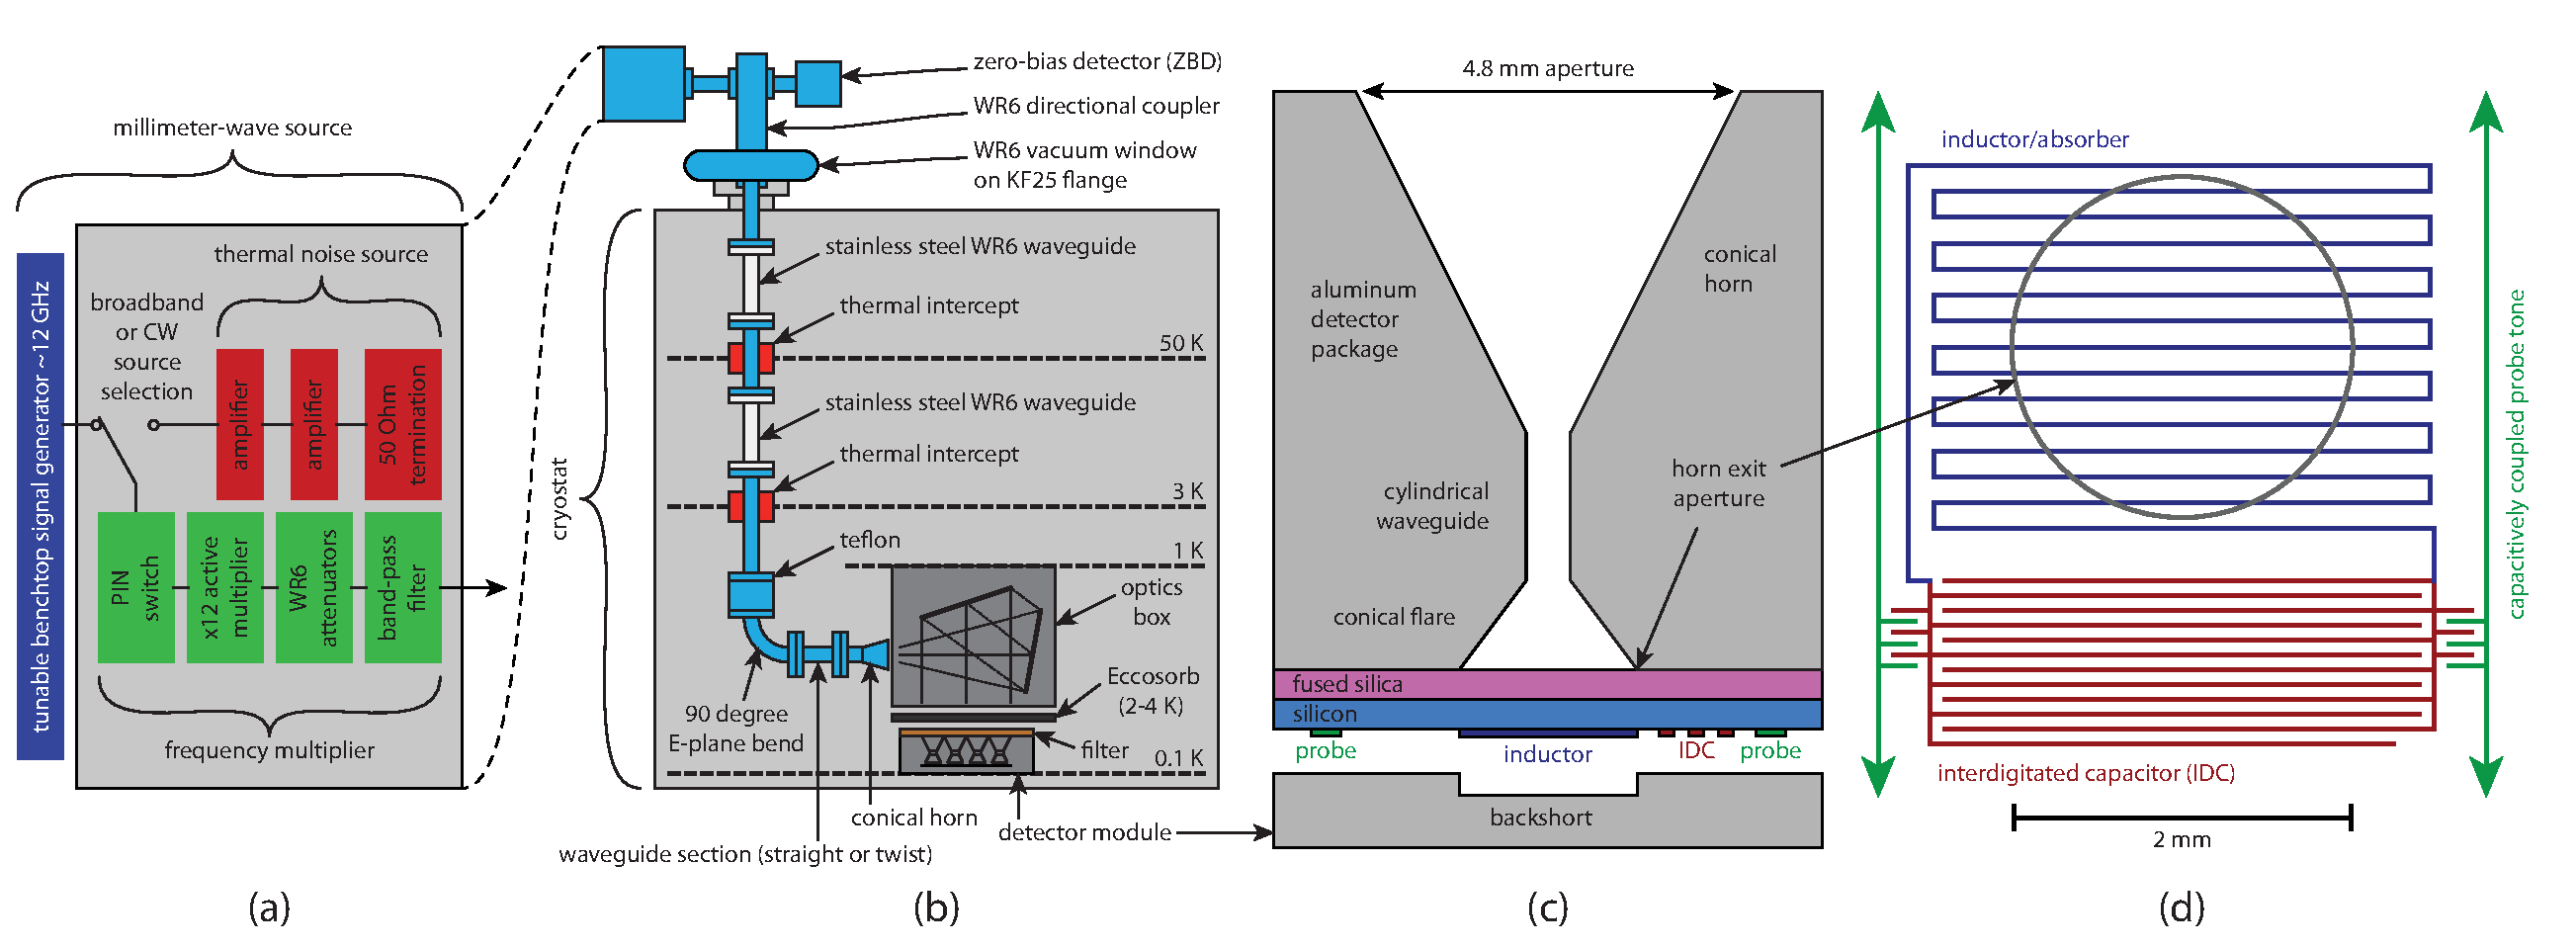
\includegraphics[width=\textwidth]{sensitivity/experiment.eps}
\caption
[Schematics of the photon noise experiment.]
{
Experiment schematics.
\textbf{(a)} The millimeter-wave source components.
\textbf{(b)} The source and cryogenic setup.
\textbf{(c)} A cross-section of an array element. The inner conical flare and fused silica layer are designed for impedance matching.
\textbf{(d)} The lumped circuit elements of one LEKID.
}
\label{fig:measuring.experiment}
\end{figure}

The array of devices used in this study was fabricated by patterning a \SI{20}{nm} aluminum film on a high-resistivity crystalline silicon substrate, with twenty detectors per array.
Each resonator comprises lithographed structures that behave electrically as lumped elements, namely an interdigitated capacitor and an inductive meander that is also the photon absorber.
Schematics of a detector and the horn coupling scheme are shown in Figure~\ref{fig:measuring.experiment}.
These devices were fabricated at STAR Cryoelectronics using the same lithographic mask used to pattern the devices described in a previous study~\autocite{McCarrick2014RSI}.
The same processing steps were used in this study except that the silicon wafer was immersed in hydrofluoric acid prior to aluminum deposition in order to clean and hydrogen-terminate the silicon surface to reduce oxide formation.
We measure a superconducting transition temperature $\tc = \SI{1.39}{K}$.
The resonance frequencies are $\SI{95}{MHz} < \freadout_\resonator < \SI{195}{MHz}$.
Under the lowest loading conditions the internal quality factors are
$\qf_\internal \approx \num{5e5} = 1 / \num{2e-6}$.
The coupling quality factors are $\qf_\coupling \approx \num{5e4} = 1 / \num{2e-5}$.
The volume of each inductive meander is \SI{1870}{\micro m^3}, assuming nominal film thickness.
The detector bath temperature is $120 \pm \SI{1}{mK}$, obtained in a cryostat using an adiabatic demagnetization refrigerator backed by a helium pulse tube cooler.
Detector readout is performed with a homodyne system using a cryogenic SiGe low-noise amplifier and open-source digital signal-processing hardware~\autocite{McCarrick2014RSI, ColumbiaCMB}.
All the data shown are from a single representative detector with $\freadout_\resonator = \SI{164}{MHz}$, and were taken at a constant readout tone power of approximately \SI{-100}{dBm} on the feedline.
The package that contains the detector chip is machined from QC-10, which is an aluminum alloy known to superconduct at the bath temperature used here.

\subsubsection{Millimeter-wave source}

Figure~\ref{fig:measuring.experiment}(a) is a schematic of the millimeter-wave source, located outside the cryostat.
Within the source, the output of a $12\times$ active multiplier chain passes through two variable waveguide attenuators that allow the output power to be controlled over a range of more than \SI{50}{dB}.
Table~\ref{tab:mmw_source} lists the primary components of the source.

The output spectrum is controlled by a band-pass filter with a sharp roll-off outside its passband of \SIrange{140}{160}{GHz}.
Within this passband, the source can produce radiation in two modes.
In \textit{broadband} mode, amplified noise is multiplied into a broadband chaotic signal.
In \textit{continuous-wave} mode, a multiplied tone from a signal generator approximates a monochromatic coherent signal.
We have measured the source output in both modes using a Fourier transform spectrometer; these measurements show that in broadband mode the power is constant within a factor of two across the output band, and in continuous-wave mode it appears monochromatic with negligible higher harmonics.

Figure~\ref{fig:measuring.experiment}(b) shows the signal path from the source through the cryostat to the detectors.
The source output is split using a waveguide directional coupler that sends 99\% of the power into a calibrated, isolator-coupled zero-bias diode power detector (ZBD), the voltage output of which is recorded using a lock-in amplifier.
The remaining 1\% of the power travels through a vacuum window and into the cryostat through WR6 waveguide.
A piece of Teflon at \SI{4}{K} inserted into the waveguide absorbs room-temperature thermal radiation.
Two mirrors transform the output of a conical horn into a collimated beam.
A \SI{6.4}{mm} thick slab of microwave absorber (Eccosorb MF-110), regulated at \SI{2}{K} during these measurements, attenuates incoming signals and provides a stable background load.
A metal-mesh filter at the detector apertures defines the upper edge of the detector band at \SI{170}{GHz}.
The lower edge of the band at \SI{130}{GHz} is defined by the cutoff frequency of a \SI{1.35}{mm} diameter circular waveguide in the detector package.
We note that the source output is within the single-mode bandwidth of both WR6 waveguide and the circular waveguide.
The radiation from the source incident on the detector horns is linearly polarized, and the electric field is aligned with the long elements of the inductive meanders in the detectors.

\begin{figure}[p]
\centering
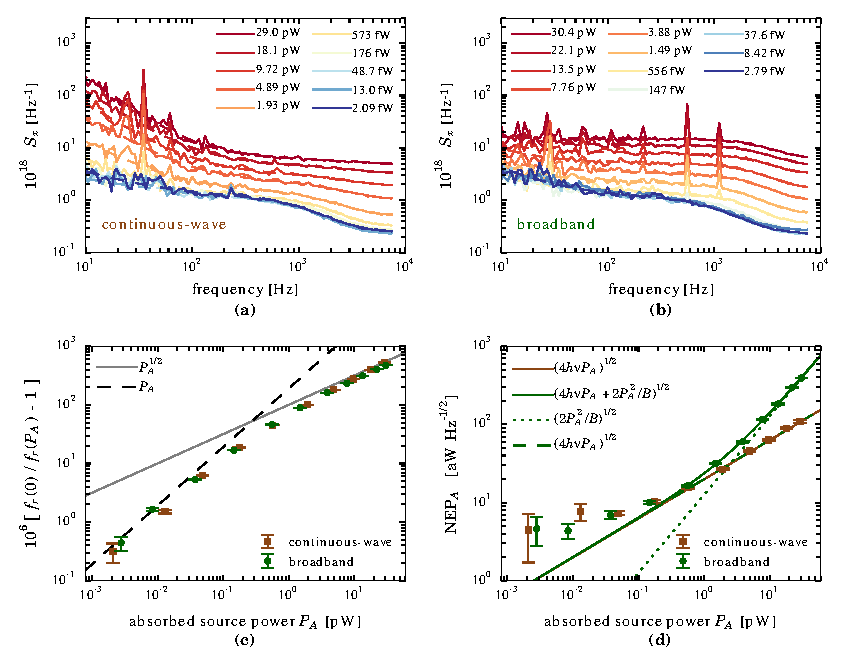
\includegraphics[width=\textwidth]{sensitivity/results.eps}
\caption
[Primary results of the photon noise experiment.]
{
Primary results of the experiment.
\textbf{(a)} Spectral density $\spectraldensity_{\detuning}$ of detector time-ordered data versus frequency under continuous-wave illumination with $\foptical = \SI{148}{GHz}$ (solid lines), and the result of fitting the data to Equation~\ref{eqn:noise_model} (dashed lines).
At high power the red noise component is dominated by fluctuations from the signal generator that feeds the multiplier; these fluctuations are correlated among detectors.
\textbf{(b)} Spectral density under broadband illumination, and fits of Equation~\ref{eqn:noise_model}.
The spikes above \SI{400}{Hz} are pickup from a fan in the source.
The red noise below \SI{100}{Hz} at low source power in both modes is produced by vibrations from the pulse tube cooler that vanish when it is turned off.
The detector white noise levels from the fits are used to calculate NEP values.
\textbf{(c)} Fractional frequency response versus absorbed power in both source modes.
The error bars are statistical errors from the resonator fits.
We use the finite-difference derivative of these response data to calculate the NEP.
The dashed black line and solid gray line are guides that show how the response scales at both low and high absorbed power.
\textbf{(d)}
Noise-equivalent power versus absorbed power in both source modes.
All data points and lines are referenced to absorbed power.
The error bars are propagated statistical errors from the finite difference derivative and the detector noise fits.
The solid green line is the sum of the quadratic and linear terms in the fit of Equation~\ref{eqn:nep} to the broadband $\nep^2$ data.
The dotted green line is the quadratic term, which is the photon wave noise contribution.
The dashed green line is the linear term, which contains equal contributions from photon shot noise and quasiparticle recombination noise.
The broadband frequency used is $\foptical = \SI{150}{GHz}$, near the band center.
The solid brown line (nearly coincident with dashed green) is the linear term in the fit of Equation~\ref{eqn:nep} to the continuous-wave $\nep^2$ data, in which the quadratic term is omitted.
}
\label{fig:measuring.results}
\end{figure}

\subsection{Results}

Figure~\ref{fig:measuring.results} shows the main results of this work.
All power values in this figure refer to the power from the source absorbed by the detector: $\power_\absorbed = \efficiency_\source \power_\source$, where $\power_\source$ is measured by the ZBD.
Before calibration, the efficiency $\efficiency_\source$ is known only approximately from measurements and simulations of the components between the source and the detector.
We accurately determine $\efficiency_\source$, and thus the absorbed source power, by measuring the relationship between emitted source power and detector noise.
This calibration relies on the assumption that all components between the source output and detector are linear: we have linearized the ZBD response at the higher power levels, all other components are passive, and we assume that filter heating is negligible.
To perform the calibration we use measurements of the noise-equivalent power (NEP), defined as the standard error of the mean in the inferred optical power at a given point in the optical system after \SI{0.5}{s} of integration~\autocite{Richards1994JAP,Zmuidzinas2003ApplOpt}.
We calculate the NEP using measurements of the detector noise and responsivity.

\subsubsection{Detector response}

At each source power level, to determine the resonance frequency and the quality factors we sweep the readout tone generator frequency $\freadout_\readout$ across a resonance and fit a resonator model to the forward scattering parameter $\forwardscattering(\freadout_\readout)$ data~\autocite{McCarrick2014RSI}.
Figure~\ref{fig:measuring.results}(c) shows the detector response to source power in both broadband and continuous-wave modes.
At low source power in both modes the fractional frequency shift
$\shift(\power_\absorbed) = \freadout_\resonator(0) / \freadout_\resonator(\power_\absorbed) - 1$ is approximately linear in power, while at high power $\shift \propto \power_\absorbed^{1/2}$.
This behavior is described by a model in which the fractional frequency shift is proportional to the number of quasiparticles:
\begin{equation}
\qpnumber
  =
  \left[ \volume (\Rate_\constant + \Rate_\source) / \qprecombinationeff \right]^{1/2},
\end{equation}
from Equation~\ref{eqn:qpnumber.response}.
Here, $\Rate_\source \propto \power_\absorbed$ is the rate of quasiparticle generation due to absorbed source photons and $\Rate_\constant$ is the constant generation rate due to other effects (such as absorption of ambient photons and thermal phonons).
We calculate the responsivity $\dv*{\detuning}{\power_\source}$ at each source power level with a finite-difference derivative that uses the fractional frequency response at adjacent power levels.


\subsubsection{Detector noise}

To measure detector noise we record time-ordered data $\forwardscattering(\freadout_\readout = \freadout_\resonator)$.
Using the resonator model from the fit to the frequency sweep we convert these data into units of detuning $\detuning$, then calculate the single-sided spectral density $\spectraldensity_{\detuning}(\faudio)$.
Figures~\ref{fig:measuring.results}(a) and \ref{fig:measuring.results}(b) show the measured noise spectra and fits to the following model:
\begin{equation}
\label{eqn:noise_model}
\spectraldensity_{\detuning}(\faudio)
  =
  \detectorwhite^2 \frac{1 + (\faudio_\knee / \faudio)^\spectralindex}{1 + (\faudio / \faudio_\cutoff)^2} + \amplifierwhite^2,
\end{equation}
where the free parameters are the detector white noise $\detectorwhite^2$, the red noise knee frequency $\faudio_\knee$, the spectral index $\spectralindex$, the cutoff frequency $\faudio_\cutoff$, and the amplifier noise $\amplifierwhite^2$.
This model treats the detector noise as the sum of a white noise process with spectral density $\detectorwhite^2$ and a red noise process with spectral density $\detectorred^2 = \detectorwhite^2 (\faudio_\knee / \faudio)^\spectralindex$, both rolled off at $\faudio_\cutoff$.

The detector bandwidth of about \SI{1}{kHz} corresponds to a limiting time constant $\tau = (2 \pi \faudio_\cutoff)^{-1}$ that is approximately equal to both the resonator ring-down time $\tau_\resonator = \qf_\resonator / \pi \freadout_\resonator$ and the expected quasiparticle relaxation time $\qprelaxationtime$ for aluminum.
Both of these time constants are expected to decrease as the absorbed optical power increases, as observed in the data.

To model the detector noise, we first consider noise sources independent of the quasiparticle system.
White noise due to the cryogenic amplifier dominates at frequencies well above the detector bandwidth, and we account for it in the model for the noise spectra.
Two-level systems (TLS) in amorphous dielectric surface layers located near the resonator produce fluctuations in the local dielectric constant and thus in $\freadout_\resonator$~\autocite{Gao2008bAPL}.
In a separate experiment, described in Section~\ref{sec:sensitivity.measuring.supplemental_material}, we determined that TLS noise is negligible at the readout power level (\SI{-100}{dBm}) used in the measurements presented here and thus do not include it in the noise model.
The chosen readout power level is high enough to suppress TLS noise but is not so high that nonlinear effects due to resonator bifurcation become significant.

The remaining noise sources involve fluctuations in the quasiparticle system: generation by optical photons, readout photons, and thermal phonons, as well as quasiparticle recombination, e.g. via phonon emission.
All of these sources are expected to produce white noise that rolls off at the frequency corresponding to the larger of $\tau_\resonator$ and $\qprelaxationtime$~\autocite{Zmuidzinas2012ARCMP}.
We expect readout generation to be negligible at high source power, and treat it as constant.
(Where present, the photon wave noise introduces correlations between photon arrival times.
This noise has a bandwidth equal to the \SI{20}{GHz} bandwidth of the absorbed broadband radiation, so it is also expected to appear white in the detector audio band~\autocite{Zmuidzinas2003ApplOpt}.)


\subsubsection{NEP model}

The NEP model includes theoretical expectations for photon noise and quasiparticle recombination noise.
We denote by $\photonoccupancy$ the mean photon occupancy of a single spatial/polarization mode of the electromagnetic field with frequency $\foptical$.
For example, for a thermal source at temperature $T$ the occupancy is
$\photonoccupancy = [\exp(\planck \foptical / \kb \temperature) - 1]^{-1}$,
where $\planck$ is Planck's constant and $\kb$ is Boltzmann's constant.
If we assume that the radiation occupies an effective optical bandwidth $\opticalbandwidth \ll \nu$ sufficiently narrow that quantities such as occupancy and absorption efficiency can be treated as constant, then the power from this mode that is absorbed by a detector with absorption efficiency $\efficiency$ is
$\power_\absorbed = \efficiency \photonoccupancy \opticalbandwidth \planck \nu$.
If the source is thermal then the contribution of photon noise to the NEP is given by~\autocite{Zmuidzinas2003ApplOpt}
\begin{equation}
\label{eqn:photon_nep}
\nep_{\absorbed, \photon}^2
  =
  2 \efficiency \photonoccupancy (1 + \efficiency \photonoccupancy) \opticalbandwidth (\planck \foptical)^2
  =
  2 \planck \foptical \power_\absorbed + 2 \power_\absorbed^2 / \opticalbandwidth,
\end{equation}
which is referenced to absorbed power.
We refer respectively to these two terms as shot noise and wave noise, following Hanbury Brown and Twiss~\autocite{HBTI1957RoyalSoc}.
If the source is monochromatic with perfect temporal coherence then only the shot noise term is present regardless of the occupancy: this behavior represents a key difference between a quantum coherent state and a quantum-statistical thermal state of the field~\autocite{Loudon2002,Glauber2006Nobel}.
For a thermal source, if $\efficiency \photonoccupancy \ll 1$ the shot noise dominates, which is typical in optical astronomy; if $\efficiency \photonoccupancy \gg 1$ the wave noise dominates, which is typical in radio astronomy.

We measure power at the output of the source and detector NEP referenced to the same point.
Referencing the photon $\nep$ to the source output gives
\begin{equation}
\label{eqn:photon_nep_source}
\nep_{\source, \photon}^2
  =
  \nep_{\absorbed, \photon}^2 / \efficiency_\source^2
  =
  2 \planck \foptical \power_\source / \efficiency_\source + 2 \power_\source^2 / \opticalbandwidth.
\end{equation}
The presence of the efficiency $\efficiency_\source$ in the linear term of this equation enables extraction of the absorbed source power.

Previous studies that calculated the absorption efficiency of a KID by measuring the scaling of photon shot noise with optical power have used superconducting films with transition temperatures similar to the film used here but larger photon energies~\autocite{Yates2011APL,Janssen2013APL,deVisser2014NatComm,Hubmayr2015APL}.
Here, the photons have energies $\planck \foptical \gtrsim 2 \gap$, where $\gap$ is the superconducting energy gap, so each photon excites only two quasiparticles close to the gap; in this limit the quasiparticle recombination noise is significant.
The recombination noise contribution to $\nep_\absorbed$ is
\begin{equation}
\label{eqn:recombination_nep}
\nep_{\absorbed, \recombination}^2
  =
  4 \gap \power_\absorbed / \pbefficiency
\end{equation}
where $\pbefficiency$ is the pair-breaking efficiency.
For photon energies $2 \gap < \planck \foptical < 4 \gap$, \textcite{deVisser2015APL} found $\pbefficiency \approx 2 \gap / \planck \foptical$, in agreement with theoretical predictions from \textcite{Guruswamy2014SUST}.
Using this value, the recombination NEP equals the shot noise term in the photon NEP.
This is expected based on the symmetry between uncorrelated pair-breaking events and uncorrelated pair-recombination events.
Finally, we introduce a small constant term $\nep_\constant$ to account for noise sources independent of source power, such as TLS noise and quasiparticle generation-recombination noise from thermal phonons, readout photons, and ambient photons.

To calculate the detector $\nep_\absorbed$, which is shown in Figure~\ref{fig:measuring.results}(d), we use the measured fractional frequency shift $\detuning$ (unitless), the measured fractional frequency noise power $\spectraldensity_{\detuning}$ (1 / Hz), and the source power $\power_\source$ (watts) as measured with a calibrated zero-bias diode (ZBD) mounted on the directional coupler outside the cryostat (see Figure 1).
The source power absorbed by the detector is related to $\power_\source$ by $\power_\absorbed = \efficiency_\source \power_\source$ where $\efficiency_\source$ is an overall system efficiency from the source output to the detector that includes the transmission through the directional coupler, the attenuation of the stainless steel waveguide, the geometrical dilution due to the internal optics, the loss in the Eccosorb, and the detector absorption efficiency.
To compute the responsivity to changes in the source power, we plot $\detuning$ versus $\power_\source$ and calculate the slope of this curve $\dv*{\detuning}{\power_\source}$ at each $\power_\source$ using a finite difference algorithm.
We use this responsivity to convert the fractional frequency noise measurements ($\spectraldensity_{\detuning}$) to $\nep_\source$.
Note that for $\nep_\source$ we use only the white noise component, $\detectorwhite$, obtained by fitting Equation~\ref{eqn:noise_model} to each $\spectraldensity_{\detuning}$ measurement.
Thus, $\nep_\source = \detectorwhite / (\dv*{\detuning}{\power_\source})$.
To convert $\power_\source$ to $\power_\absorbed$ we need to determine $\efficiency_\source$.
The complete theoretical model for $\nep_\source$ is
\begin{align}
\begin{split}
\label{eqn:nep}
\nep_\source^2
  &=
  (\nep_{\absorbed, \constant}^2
   + \nep_{\absorbed, \recombination}^2
   + \nep_{\absorbed, \photon}^2) / \efficiency_\source^2 \\
  &=
  \nep_{\absorbed, \constant}^2 / \efficiency_\source^2
  + [2 (2 \planck \foptical \power_\absorbed) + 2 \power_\absorbed^2 / \opticalbandwidth] / \efficiency_\source^2 \\
  &=
  \nep_{\source, \constant}^2
  + 4 \planck \foptical \power_\source / \efficiency_\source
  + 2 \power_\source^2 / \opticalbandwidth,
\end{split}
\end{align}
which is the sum of the aforementioned noise contributions.
The right-hand side of this equation is quadratic in $P_\source$ with unknown quantities $\nep_{\source, \constant}$, $\efficiency_\source$, and effective optical bandwidth $\opticalbandwidth$.
The limiting $\nep_{\source, \constant}$ is discussed below.
We fit Equation~\ref{eqn:nep} to the broadband data using center frequency $\foptical = \SI{150}{GHz}$ and obtain $\efficiency_\source = \num{8.50e-7} (1 \pm 0.09)$ and $\opticalbandwidth = \SI{13}{GHz}$.
The quadratic term is not expected to be present for coherent illumination because the source should produce only shot noise, so we fit Equation~\ref{eqn:nep} to the continuous-wave data omitting the third term.
Here, $\foptical = \SI{148}{GHz}$ and we obtain $\efficiency_\source = \num{1.12e-6} (1 \pm
0.04)$.
As a final step, we convert $\power_\source$ to $\power_\absorbed$ using the $\efficiency_\source$ values from the model fitting and produce Figures~\ref{fig:measuring.results}(c) and \ref{fig:measuring.results}(d).
Note that because the broadband source involves contributions from the full source output bandwidth, it is not surprising that the measured $\efficiency_\source$ values differ between the continuous-wave and broadband modes by more than the statistical error bars.

\subsection{Discussion}

Figure~\ref{fig:measuring.results}(d) shows that photon noise dominates under broadband illumination when
$\power_\absorbed \gtrsim \SI{1}{pW}$,
which corresponds to 
$\nep_\absorbed \approx \SI{2e-17}{W.Hz^{-1/2}}$.
At high power in each source mode we observe the expected relationship between noise and power: in broadband mode $\nep \propto \power$ because the quadratic wave noise term dominates, while in continuous-wave mode $\nep \propto \power^{1/2}$ because the quadratic term is not present.
This behavior is a clear signature of photon noise.

Note that the the $\nep_\absorbed$ values reported have the amplifier noise contribution subtracted because the white noise parameter $W^2$ in Equation~\ref{eqn:noise_model} describes the noise power above the amplifier noise $\amplifierwhite^2$.
Here, subtracting the amplifier noise yields an accurate estimate of the detector performance because, alternatively, the amplifier noise can be suppressed to a negligible level by increasing the readout power.
We verified both approaches yield the same $\nep_\absorbed$ versus $\power_\absorbed$ result but chose to report the amplifier-noise-subtracted results.

At low absorbed source power levels in both modes, where $\power_\absorbed < \SI{0.1}{pW}$, $\nep_\absorbed$ levels off to $\nep_\constant$.
The values of $\nep_\constant$ extracted from both of the aforementioned fits are approximately 5 to \SI{6e-18}{W.Hz^{-1/2}}.
To explain this leveling-off effect, we model the background loading as emission from a black body at \SI{2}{K}, which is the temperature of the Eccosorb in front of the feed horn apertures.
Assuming center frequency $\foptical = \SI{150}{GHz}$, measured filter transmission $\efficiency_\mathrm{F}(\nu) = 0.94$, optical efficiency $\efficiency_\incident = 0.7$ (obtained from electromagnetic simulations), and detector bandwidth $\opticalbandwidth_\mathrm{full} = \SI{40}{GHz}$, then the radiative loading from the Eccosorb is 
\begin{equation*}
\power_\absorbed
  =
  \efficiency_\incident \photonoccupancy(\foptical, \SI{2}{K}) \planck \foptical \opticalbandwidth_\mathrm{full} = \SI{0.08}{pW}.
\end{equation*}
This loading level is close to the observed knee in the curves in Figure~\ref{fig:measuring.results}(d).
Adding an equal recombination noise contribution to the corresponding photon NEP results in
\begin{equation}
\nep_\absorbed = (2 \cdot 2 \planck \foptical \power_\absorbed)^{1/2} = \SI{5.6e-18}{W.Hz^{-1/2}},
\end{equation}
which is close to the observed $\nep_\constant$ value.
Therefore, the observed limiting $\nep_\absorbed$ is consistent with this model of the expected background loading.

Analysis of data from twelve detectors yielded similar results to those shown in Figure~\ref{fig:measuring.results}(d), with the photon noise starting to dominate between 0.5 and \SI{1}{pW}.
We conclude that these detectors become limited by photon noise at absorbed power levels lower than the background power levels already measured by ground-based CMB polarimeters~\autocite{BICEP2II2014ApJ}.


\subsection{Supplemental material}
\label{sec:sensitivity.measuring.supplemental_material}

The contents of this section were presented as supplemental material for the published paper.
The content that is specific to the paper is retained here, while the more general content has been moved earlier in this chapter.

\subsubsection{Two-level system noise}

At low temperatures we see evidence for TLS effects in measurements of resonance frequency versus bath temperature, which depart from the Mattis-Bardeen prediction, and in the fact that the internal quality factors increase with increasing readout power.
The connection between these steady-state TLS effects and TLS noise is not fully understood.
The method we used to estimate the TLS noise contribution is described in this section.
We conclude that TLS noise is negligible and thus do not include it explicitly in the analysis of the NEP.

The importance of modeling TLS noise to avoid a systematic error in this measurement is explained in Section~\ref{sec:sensitivity.tls}.
The TLS contribution to the spectral density is given by 
Equation~\ref{eqn:spectraldensity_tls}.
The experiment described in the main text is performed with constant readout power $\power_\readout$ on the feedline, and we expect the TLS noise level to vary as $\power_\internal^{-1/2} = (\chi_a \power_\readout)^{-1/2}$, where $\chi_a \le 1/2$, which can be calculated from the resonator parameters, is the fraction of readout power that flows into the resonator~\autocite{Zmuidzinas2012ARCMP}.

\begin{figure}[htb]
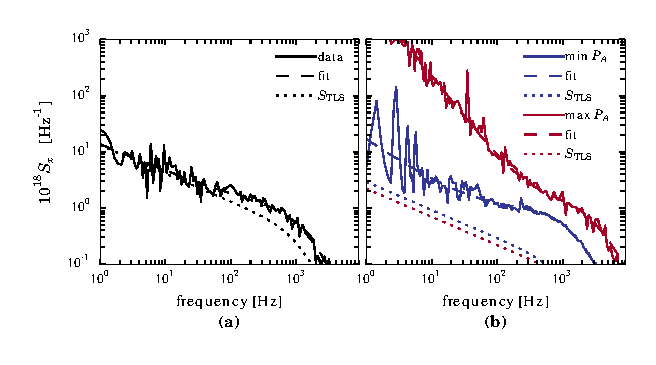
\includegraphics[width=\columnwidth]{sensitivity/dark_and_light_noise_minus_amp_two_panel.eps}
\caption
[Dark noise data and fits.]
{
\textbf{(a)}
Amplifier-subtracted dark noise data for the same detector characterized in the main text.
The dashed line shows a fit to the same model used in the main text, except that here the spectral index is fixed to $\spectralindex = 0.5$ to match a possible TLS contribution.
To show the detector noise more clearly, the amplifier noise value obtained from the fit has been subtracted from the data and fit curves.
The dotted line shows the possible TLS contribution, assumed to roll off with the same time constant obtained from the fit.
\textbf{(b)}
Amplifier-subtracted illuminated continuous-wave noise data.
The solid lines shown here are the lowest and highest power curves from Figure~\ref{fig:measuring.results}(a), and the dashed lines are the same fits shown in the main text, except that the amplifier noise values obtained from the fits have been subtracted from the data and fit curves.
The dotted lines are the inferred TLS contribution to the illuminated spectra, scaled from the fit value in panel (a) by a factor $(\power_{\internal, \dark} / \power_\internal)^{1/2}$.
The TLS contribution in this case decreases as source power increases.}
\label{fig:measuring.dark_noise}
\end{figure}

In order to estimate the TLS contribution to the NEP, we performed a separate experiment in which we attempted to make the TLS noise as prominent as possible.
Three key aspects differ from the experiment described in the main text: the horn apertures were covered with aluminum tape to minimize optical loading; the readout power was approximately \SI{-112}{dBm}, \SI{12}{dB} lower than in the primary experiment; in order to remove noise due to vibrations caused by the pulse tube cooler, we turned it off to record time-ordered data while the adiabatic demagnetization refrigerator continued to regulate the bath temperature at \SI{120}{mK}.

Figure~\ref{fig:measuring.dark_noise}(a) shows the detuning spectral density taken under these dark conditions and a fit used to extract a possible TLS noise contribution.
Figure~\ref{fig:measuring.dark_noise}(b) shows that this TLS contribution is negligible when adjusted for the increased readout power used in the primary experiment.


\subsubsection{Spectral density fitting}

\begin{table}[htb]
\centering
\caption
[Best-fit parameters from the spectral density fits of the broadband data.]
{Broadband best-fit parameters with uncertainties.
At high power, because the noise is very close to white, the red noise contribution is negligible and the parameters ($\faudio_\knee$ and $\spectralindex$) that describe the red noise are poorly constrained; the white noise $\detectorwhite^2$ is still well constrained.}
\renewcommand{\arraystretch}{1.2}
\begin{tabular}{cccccc}
\toprule
$\power_\absorbed$ & $\amplifierwhite^2 / \SI{e-18}{Hz^{-1}}$ & $\detectorwhite^2 / \SI{e-18}{Hz^{-1}}$ & $\faudio_\knee / \si{Hz}$ & $\spectralindex$ & $\faudio_\cutoff / \si{kHz}$ \\
\midrule
\SI{30.4}{pW} & 5.2 $\pm$ 0.1 & 10.0 $\pm$ 0.2 & 0 $\pm$ 20 & 1 $\pm$ 6 & 3.0 $\pm$ 0.1 \\
\SI{22.1}{pW} & 3.9 $\pm$ 0.1 & 7.7 $\pm$ 0.1 & 11 $\pm$ 3 & 1.9 $\pm$ 0.9 & 2.9 $\pm$ 0.1 \\
\SI{13.5}{pW} & 2.67 $\pm$ 0.06 & 5.3 $\pm$ 0.1 & 7 $\pm$ 4 & 1.0 $\pm$ 0.5 & 2.7 $\pm$ 0.1 \\
\SI{7.76}{pW} & 1.38 $\pm$ 0.03 & 3.81 $\pm$ 0.08 & 12 $\pm$ 3 & 1.2 $\pm$ 0.4 & 2.48 $\pm$ 0.08 \\
\SI{3.88}{pW} & 0.82 $\pm$ 0.02 & 2.4 $\pm$ 0.1 & 9 $\pm$ 4 & 0.8 $\pm$ 0.3 & 2.34 $\pm$ 0.10 \\
\SI{1.49}{pW} & 0.481 $\pm$ 0.007 & 1.73 $\pm$ 0.05 & 14 $\pm$ 3 & 1.2 $\pm$ 0.3 & 1.80 $\pm$ 0.05 \\
\SI{556}{fW} & 0.309 $\pm$ 0.005 & 1.11 $\pm$ 0.04 & 13 $\pm$ 3 & 1.0 $\pm$ 0.3 & 1.70 $\pm$ 0.06 \\
\SI{147}{fW} & 0.229 $\pm$ 0.002 & 0.98 $\pm$ 0.03 & 21 $\pm$ 2 & 1.2 $\pm$ 0.2 & 1.29 $\pm$ 0.03 \\
\SI{37.6}{fW} & 0.201 $\pm$ 0.002 & 0.69 $\pm$ 0.09 & 60 $\pm$ 20 & 0.7 $\pm$ 0.1 & 1.24 $\pm$ 0.07 \\
\SI{8.42}{fW} & 0.247 $\pm$ 0.002 & 0.77 $\pm$ 0.08 & 60 $\pm$ 20 & 0.7 $\pm$ 0.1 & 1.14 $\pm$ 0.05 \\
\SI{2.79}{fW} & 0.213 $\pm$ 0.002 & 0.89 $\pm$ 0.05 & 34 $\pm$ 5 & 1.0 $\pm$ 0.2 & 1.06 $\pm$ 0.04 \\
\bottomrule
\end{tabular}
\label{tab:bbfitparams}
\end{table}

\begin{table}[t]
\centering
\caption
[Best-fit parameters from the spectral density fits of the continuous-wave data.]
{Continuous-wave best-fit parameters with uncertainties.}
\renewcommand{\arraystretch}{1.2}
\begin{tabular}{cccccc}
\toprule
$\power_\absorbed$ & $\amplifierwhite^2 / \SI{e-18}{Hz^{-1}}$ & $\detectorwhite^2 / \SI{e-18}{Hz^{-1}}$ & $\faudio_\knee / \si{Hz}$ & $\spectralindex$ & $\faudio_\cutoff / \si{kHz}$ \\
\midrule
\SI{29.0}{pW} & 4.89 $\pm$ 0.06 & 1.3 $\pm$ 0.1 & 330 $\pm$ 40 & 1.46 $\pm$ 0.05 & 2.5 $\pm$ 0.4 \\
\SI{18.1}{pW} & 3.20 $\pm$ 0.04 & 1.46 $\pm$ 0.09 & 270 $\pm$ 30 & 1.33 $\pm$ 0.05 & 2.6 $\pm$ 0.3 \\
\SI{9.72}{pW} & 1.82 $\pm$ 0.03 & 1.27 $\pm$ 0.07 & 220 $\pm$ 30 & 1.28 $\pm$ 0.06 & 2.4 $\pm$ 0.2 \\
\SI{4.89}{pW} & 0.98 $\pm$ 0.01 & 1.22 $\pm$ 0.05 & 160 $\pm$ 20 & 1.25 $\pm$ 0.06 & 2.2 $\pm$ 0.1 \\
\SI{1.93}{pW} & 0.462 $\pm$ 0.006 & 0.97 $\pm$ 0.04 & 100 $\pm$ 10 & 1.09 $\pm$ 0.07 & 1.83 $\pm$ 0.07 \\
\SI{573}{fW} & 0.288 $\pm$ 0.003 & 0.87 $\pm$ 0.04 & 52 $\pm$ 7 & 1.1 $\pm$ 0.1 & 1.56 $\pm$ 0.05 \\
\SI{176}{fW} & 0.244 $\pm$ 0.003 & 0.88 $\pm$ 0.06 & 37 $\pm$ 8 & 0.9 $\pm$ 0.2 & 1.29 $\pm$ 0.05 \\
\SI{48.7}{fW} & 0.219 $\pm$ 0.002 & 0.82 $\pm$ 0.05 & 39 $\pm$ 7 & 1.0 $\pm$ 0.1 & 1.21 $\pm$ 0.05 \\
\SI{13.0}{fW} & 0.210 $\pm$ 0.002 & 0.7 $\pm$ 0.2 & 40 $\pm$ 40 & 0.6 $\pm$ 0.2 & 1.17 $\pm$ 0.08 \\
\SI{2.09}{fW} & 0.235 $\pm$ 0.002 & 0.85 $\pm$ 0.08 & 40 $\pm$ 10 & 0.8 $\pm$ 0.2 & 1.13 $\pm$ 0.05 \\
\bottomrule
\end{tabular}
\label{tab:cwfitparams}
\end{table}

In this section we provide details of the procedure used to fit the spectral density to Equation~\ref{eqn:noise_model}.
To estimate the spectral density of the time-ordered fractional frequency shift data we first use Welch's average periodogram method with the data split into 16 equal non-overlapping chunks.
This produces a single-sided spectral density that is the average of 16 spectra.
We estimate the variance of point $j$ with value $\spectraldensity_j$ by $\sigma_j^2 = \spectraldensity_j^2 / 16$.
We then bin this spectrum using bin widths that increase with frequency, and propagate the errors by adding the variances in quadrature.
These binned spectra are plotted in Figures~\ref{fig:measuring.results}(a) and \ref{fig:measuring.results}(b).

This binning and averaging procedure produces $\chi^2$ distributed data with $2 \times 16 \times n_k$ degrees of freedom, where $n_k$ is the number of points that are averaged in bin $k$.
The resulting distribution closely approximates a Gaussian distribution~\autocite{Norrelykke2010RSI}, even for $n_k = 1$.
To fit the model to the data we use a least-squares fitting routine with the squared residual at each frequency point weighted by the inverse of the variance in that bin.
Only data at frequencies above \SI{10}{Hz} is used in the fits.
This model will over-describe the data if the spectrum has no red noise or no white noise component, in which case the uncertainties on the remaining parameters would be underestimated.
The resulting best-fit parameters are listed in Tables~\ref{tab:bbfitparams}~and~\ref{tab:cwfitparams}.

\chapter{Multichroic detectors}
\label{chp:multichroic}

This chapter describes a project to develop arrays of polarization-sensitive, multichroic KID pixels for future CMB experiments.
These detectors are designed to help separate foreground signals from CMB signals by measuring two spectral bands simultaneously.
One band is primarily for detecting the CMB, so it is centered on \SI{150}{GHz}, near the peak of the CMB black body spectrum.
The other band is primarily for detecting Galactic dust signals, so it is centered on \SI{235}{GHz}, where the dust emission is brighter than the CMB.
Some of the material in this chapter was published in \textcite{Johnson2016SPIE} and \textcite{Johnson2017arXiv}.


\section{Overview}
\label{sec:multichroic.overview}

The pixels are each sensitive to two linear polarization states in two spectral bands, so there are four KIDs per pixel.
Each pixel consists of a feedhorn, waveguide, and ortho-mode transducer (OMT) antenna that together couple light from free space onto the chip; microstrip (MS) millimeter-wave circuits that filter and route the light; and four hybrid aluminum-niobium co-planar waveguide (CPW) KIDs that detect the light.
Figure~\ref{fig:multichroic_mkid_coupling_v3} shows drawings of the design.

\begin{figure}[htb]
\centering
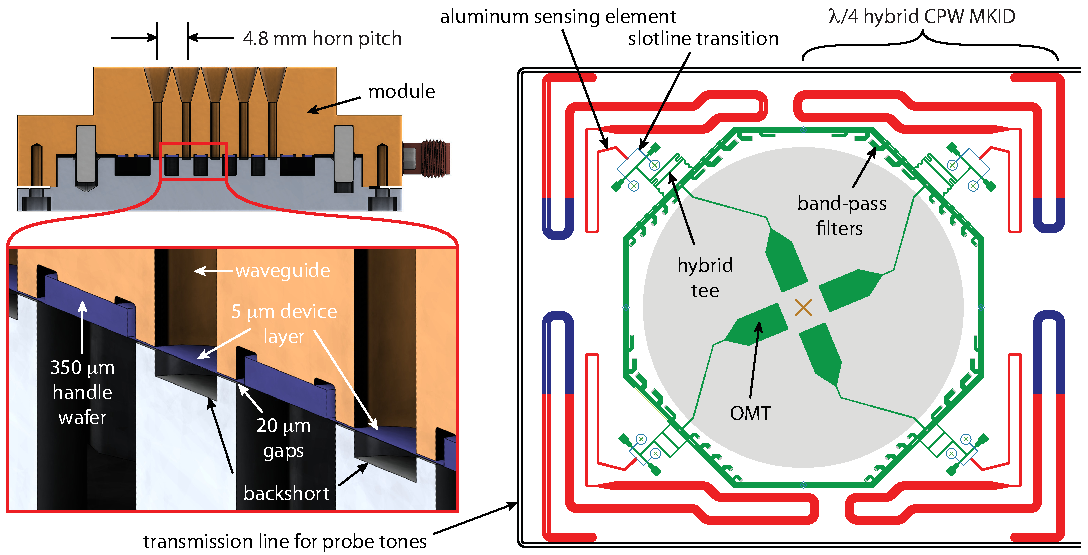
\includegraphics[width=\textwidth]{multichroic/multichroic_mkid_coupling_v3.pdf}
\caption[Drawings of the multichroic detector module and of one multichroic pixel.]
{
\textbf{(Left)}
A drawing of the multichroic detector module.
The upper panel shows a cross-section of the entire module.
The detector wafer (blue) is enclosed between the two aluminum pieces (brown and gray).
Light enters the feedhorns at the top and propagates down the circular waveguide.
The lower panel shows detail of the area where light couples to the OMT antennas, which from this perspective would appear on the underside of the blue membranes.
The bosses that extend the waveguide toward the wafer from both sides form chokes that reduce lateral leakage of light.
The backshorts terminate the waveguides and improve the optical coupling.
\textbf{(Right)}
A drawing of one multichroic pixel.
The two opposing OMT probe pairs (green) in the center of the pixel are sensitive to orthogonal linear polarization states.
The band-pass filters and hybrid (\SI{180}{\degree}) tee, which are microstrip components, create the two spectral bands and combine the signals to select the desired waveguide mode.
The slotline transition couples the light from the microstrip circuitry into the aluminum CPW sensing region of one of the quarter-wavelength CPW KIDs.
The region of the KIDs drawn in red is the same in each pixel, while the region drawn in blue varies in order to set the resonance frequency.
The resonators are weakly coupled to the feedline, shown in gray, by the short lengths (``elbow couplers'') of transmission line that run parallel to it.
This figure was published in \textcite{Johnson2017arXiv}.
}
\label{fig:multichroic_mkid_coupling_v3}
\end{figure}

Our design was based on detectors that were developed for~\autocite{Datta2014JLTP, Henderson2016JLTP, Duff2016JLTP} and deployed on~\autocite{Ho2016JLTP,Datta2016JLTP} the Advanced ACTPol experiment~\autocite{Thornton2016ApJS}, which is a CMB polarization experiment on the Atacama Cosmology Telescope (ACT) in northern Chile~\autocite{ACT2011ApJS}.
Our goal was to replace the bolometers used by ACTPol with KIDs.
For reasons described below, we chose to use silicon-on-insulator (SOI) wafers instead of the dielectrics used in the ACTPol design.
We also chose to replace the ring-loaded ACTPol feedhorns with conical feedhorns, for simplicity of fabrication.
Thus, the initial design tasks were as follows.
First, to re-optimize the feedhorn coupling scheme and millimeter-wave circuitry for SOI.
Second, to develop a circuit to couple the optical radiation from the microstrip circuitry to the KID CPW center strip.
Third, to design and draw CPW resonators with suitable resonance frequencies within the available chip area.
Fourth, to design a metal package to enclose the wafer using the new optical design.
The first two tasks were done by collaborators, and the latter two were primarily my responsibilities.


\section{Optical coupling}
\label{sec:multichroic.optical}

In our prototype design, a conical horn with a \SI{4.66}{mm} diameter aperture and a \SI{15}{\degree} flare angle is used to feed each pixel.
Each horn feeds a \SI{1.49}{mm} diameter circular waveguide that is made approximately \SI{9}{mm} long to ensure that evanescent low-frequency modes do not reach the detectors.
A broadband planar waveguide probe OMT on a thin membrane separates orthogonal linear polarizations.
The orientation of the OMT defines a polarimeter axis that is independent of frequency.
Chokes on both sides of the membrane reduce lateral leakage into the module.
A backshort behind the membrane reflects light that was not absorbed on the first pass, which improves the optical coupling.
Figure~\ref{fig:multichroic_mkid_coupling_v3} shows detail of these structures.

\begin{figure}[htb]
\centering
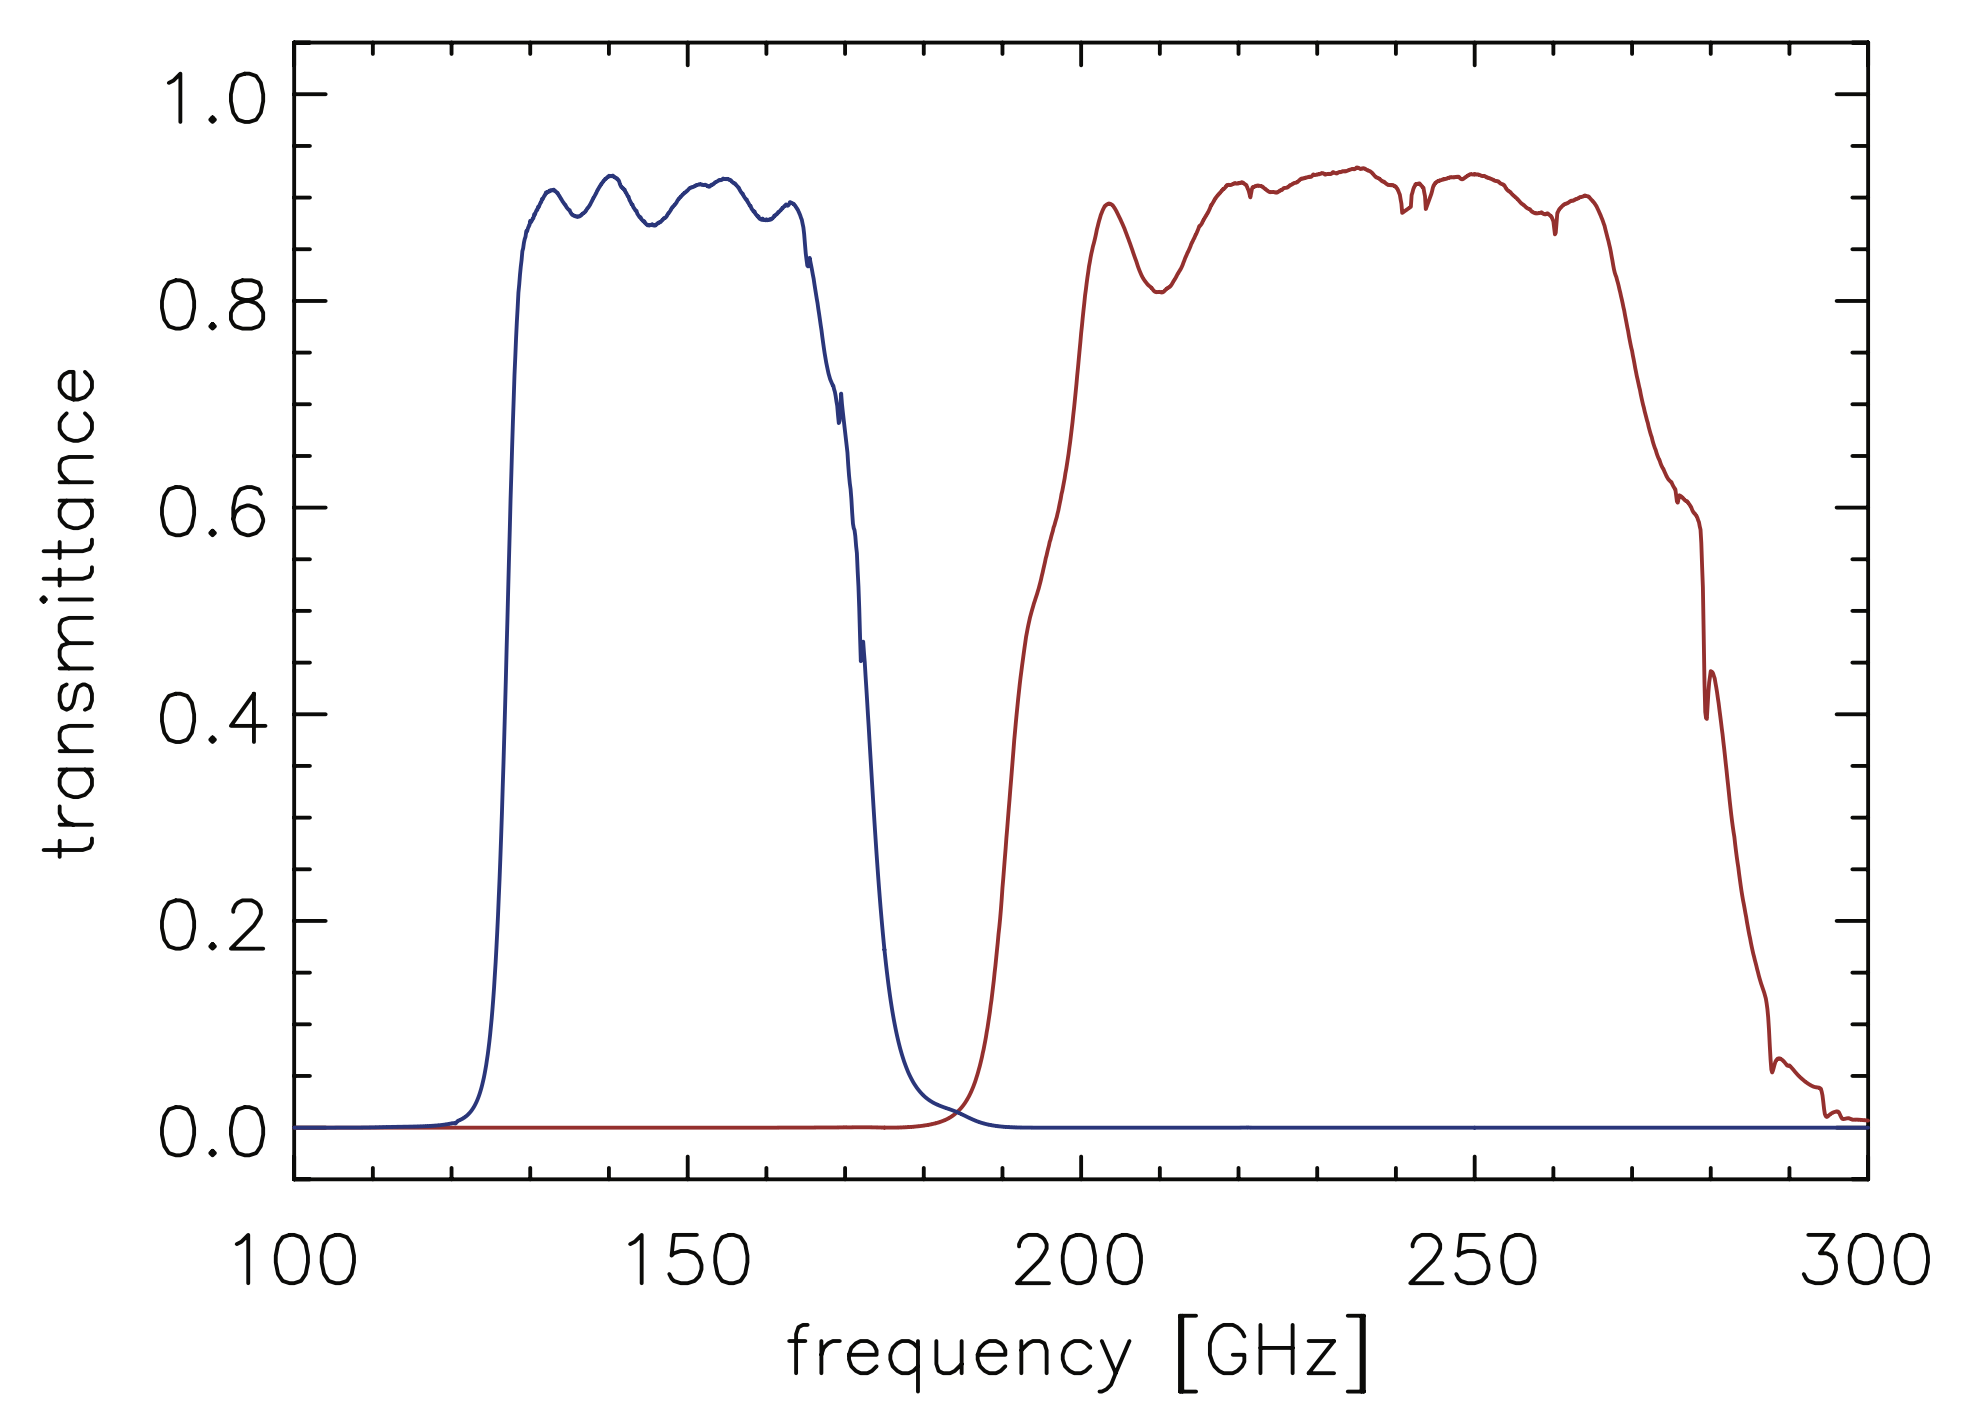
\includegraphics[width=0.8\textwidth]{multichroic/multichroic_spectral_bands.png}
\caption[Simulations of the spectral bands for the multichroic KID pixels.]
{
Simulations of the spectral bands for the multichroic KID pixels.
This figure was published in \textcite{Johnson2016SPIE}.
}
\label{fig:multichroic_spectral_bands}
\end{figure}

The output of each waveguide probe is CPW, so a broadband CPW-to-MS transition composed of seven alternating sections couples light to the on-chip MS circuitry.
A diplexer consisting of two sets of five-pole resonant-stub MS band-pass filters splits the light into the two spectral bands, \SIrange{125}{170}{GHz} and \SIrange{190}{280}{GHz}.
The results of end-to-end electromagnetic simulations, shown in 
Figure~\ref{fig:multichroic_spectral_bands}, indicate that the expected absorption efficiency is approximately 0.9 across the 150 GHz and the 235 GHz spectral bands.
Circular waveguide supports multiple modes over this fractional bandwidth of 2.25:1, but only the TE$_{11}$ mode has desirable polarization properties.
This mode couples to opposite fins of the OMT with a \SI{180}{\degree} phase shift, while the next highest order mode, which also couples efficiently to the OMT probes, has a \SI{0}{\degree} phase shift.
A \SI{180}{\degree} hybrid combines the light from each probe pair within a single spectral band, and the path lengths from the probes to the inputs of the hybrid are designed to be identical.
To ensure single-mode performance, the sum port of the hybrid is terminated in a resistive gold microstrip, while the difference port is connected to the KID using a broadband coupling circuit that is described below.
To re-optimize the feedhorn coupling and the millimeter-wave circuitry, our collaborators at the University of Michigan performed electromagnetic simulation of the components using ANSYS HFSS software~\autocite{HFSS} and Sonnet EM software~\autocite{Sonnet}. % Jeff McMahon and Rahul Datta

\begin{figure}[htb]
\centering
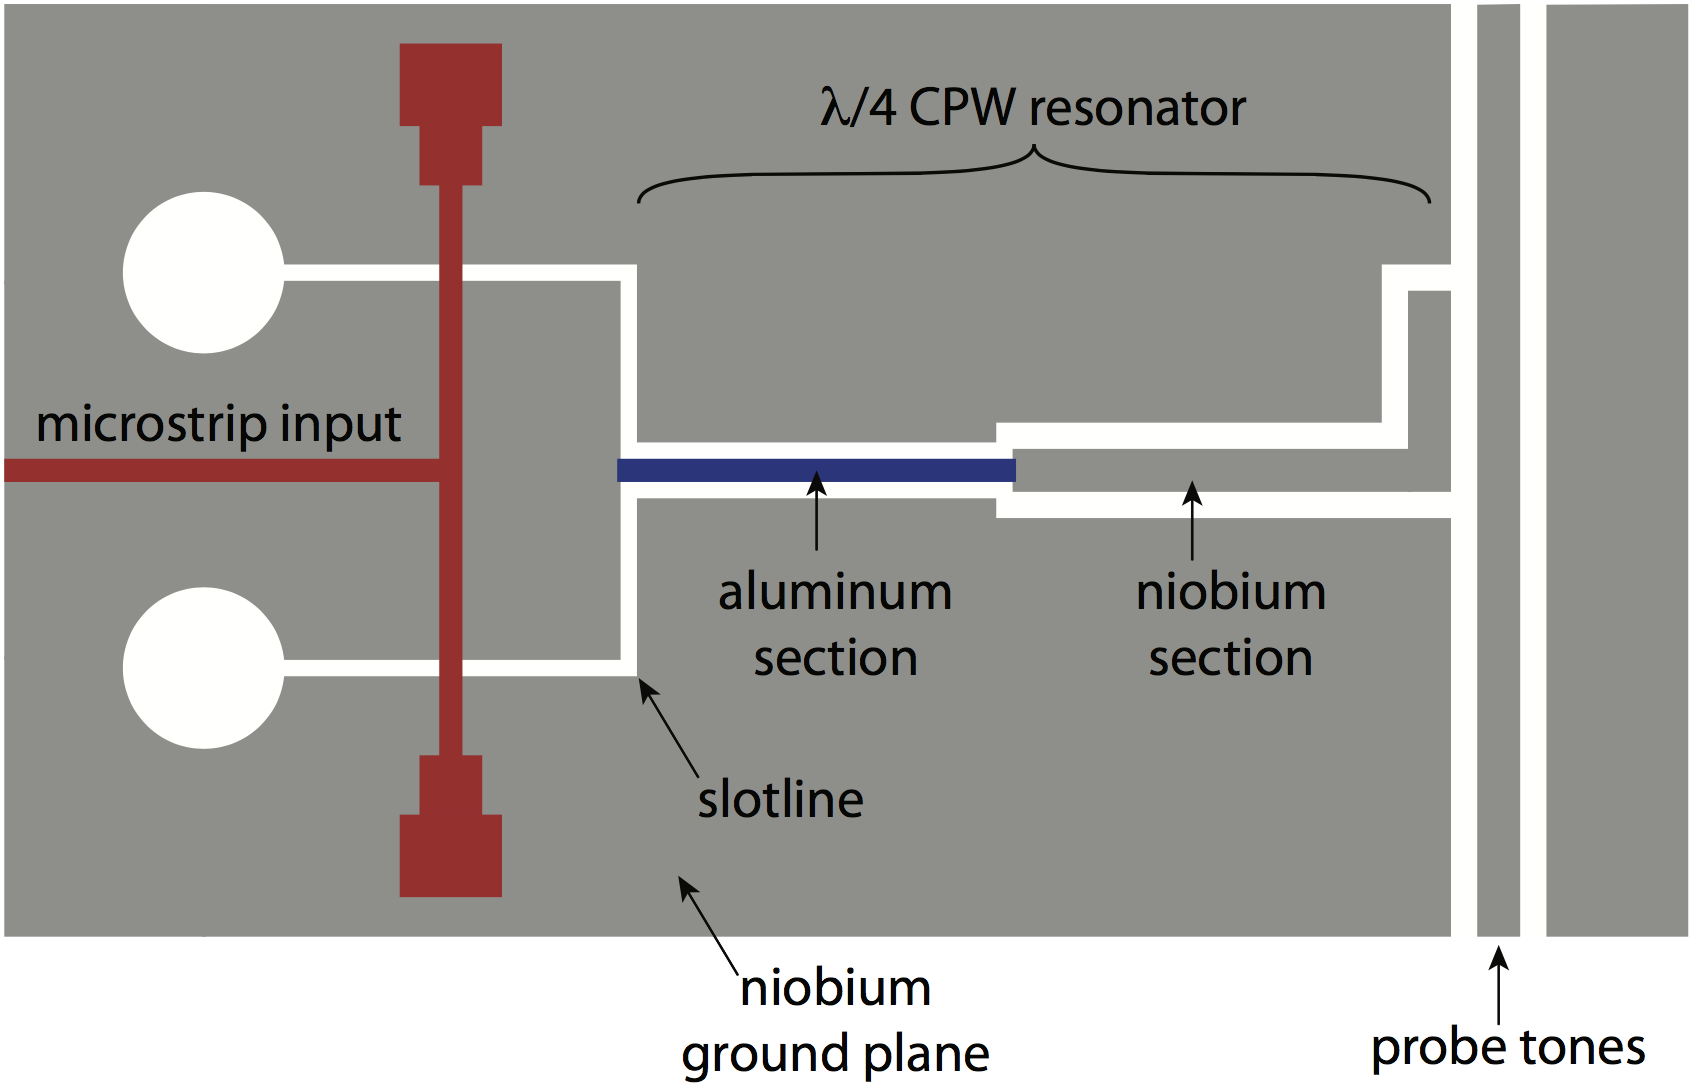
\includegraphics[width=0.7\textwidth]{multichroic/multichroic_ms-to-cpw_coupler_schematic.png}
\caption[A schematic of the microstrip-to-coplanar-waveguide coupler for the multichroic KID project.]
{
A schematic of the microstrip-to-coplanar-waveguide coupler for the multichroic KID project.
This figure was published in \textcite{Johnson2016SPIE}
}
\label{fig:multichroic_ms-to-cpw_coupler_schematic}
\end{figure}

Our collaborators at Arizona State University designed a MS-to-CPW coupler and optimized it using Sonnet simulations that are described by \textcite{Surdi2016}.  % Philip Mauskopf and Harshad Surdi 
Figure~\ref{fig:multichroic_ms-to-cpw_coupler_schematic} is a schematic of the coupler.
Millimeter-wave light coming from the microstrip output of the \SI{180}{\degree} hybrid is evenly divided in-phase onto two microstrip branches that each have twice the impedance of the input.
Each branch feeds a standard broadband microstrip-to-slotline transition that couples the light into a slotline formed in the ground plane.
The two slotlines come together and meet the CPW gaps in the aluminum section of the MKID.


\section{Prototype resonators: simulation and testing}
\label{sec:multichroic.prototype}

Since the millimeter-wave circuitry required a niobium ground plane, a hybrid KID design was a natural choice.
A hybrid KID is made from two superconductors with different gap energies.
One superconductor, the \textit{active} metal, must have a spectroscopic gap below the photon energy so that optical photons can break pairs in this region of the resonator.
The other superconductor, the \textit{inactive} metal, should have a higher gap so that optically excited quasiparticles in the active region remain trapped there.
In the design presented here, in which optical photons propagate on transmission lines made from the inactive metal, its spectroscopic gap must be higher than the photon energy so that these photons can propagate without loss.
Optically-excited quasiparticles are trapped in the active region since their energies are less than the gap in the inactive metal.

We chose to use CPW resonators with an aluminum active region because hybrid CPW KIDs (using aluminum and niobium-titanium-nitride) have demonstrated excellent sensitivity~\autocite{Yates2011APL,Janssen2013APL,Janssen2014SPIE} and have been incorporated into large arrays~\autocite{Baselmans2017AA}.
The ACTPol OMTs were fabricated on a low-stress silicon nitride (SiN$_x$) membrane formed by etching away the silicon wafer beneath.
Because amorphous dielectrics tend to produce excess loss (Section~\ref{sec:loss.dielectrics}) and noise (Section~\ref{sec:sensitivity.tls}) in KIDs, we decided to avoid using a silicon nitride membrane.
Instead, we planned to use a SOI wafer that consists of a thin crystalline silicon device layer above a thin silicon oxide (SiO$_2$) layer above a thick crystalline silicon handle layer that provides mechanical support.
The membrane would be formed by etching away the dielectrics beneath the device layer.
Lossy dielectrics underneath the KIDs would also be etched away as required.

While transmission-line resonators are a common choice for KIDs, when this project began my group had designed and fabricated only lumped-element resonators.
The starting point for analysis of a CPW resonator is that the structure supports a quasi-transverse electromagnetic (quasi-TEM) mode.
The wave speed $\lightspeed$ for this mode can be approximated using the average dielectric constant of the substrate $\epsilon_\mathrm{substrate}$ and of vacuum~\autocite{Wen1969IEEE}:
\begin{equation}
\lightspeed
  =
  \lsvac \left( \frac{1 + \epsilon_\mathrm{substrate}}{2} \right)^{-1/2},
\end{equation}
where $\lsvac$ is the speed of light in vacuum.
Silicon has dielectric constant $\epsilon = 11.9$ at microwave frequencies.
The length of a quarter-wavelength resonator with a given resonance frequency $\freadout_\resonator$ is thus
\begin{equation}
\tracelength
  =
  \wavelength / 4
  =
  \freadout_\resonator / 4 \lightspeed.
\end{equation}
The wave speed is reduced if the CPW is made from a superconducting structure with significant kinetic inductance, and the resonance frequency shifts accordingly:
\begin{equation}
\freadout_\resonator
  =
  \left(1 - \kifraction \right)^{1/2} \freadout_\resonator(\kifraction = 0).
\end{equation}
\todo[inline]{Discuss calculation of kinetic inductance fraction}
The effective kinetic inductance fraction $\kifraction$ is not trivial to calculate for hybrid resonators.
\textcite{Gao2008} discusses the effective kinetic inductance fraction of superconducting CPW resonators in detail.
\todo[inline]{Use estimates from for center-only and shorted end only}

I used electromagnetic simulations~\autocite{Sonnet} to simulate hybrid quarter-wavelength CPW resonators in order to validate the design and estimate the effective kinetic inductance fraction.
To find the resonance frequencies quickly I used a three-port method~\autocite{Wisbey2014JLTP}, which involves inserting a third port in the CPW center trace where it meets the ground plane, in addition to the two ports on the feedline.
Our heterodyne system can read out resonances up to about \SI{4}{GHz}.
As discussed in Chapter~\ref{chp:theory}, the fractional frequency response is enhanced at lower resonance frequencies, so I targeted frequencies around \SI{3}{GHz}.
In order to achieve the desired resonance frequencies in the limited area that was available, it was necessary to fold the resonators into the shape shown in Figure~\ref{fig:mkidarray01-0101_photo_one_resonator}, which is a photograph of a fabricated resonator.
This exact geometry was too computationally expensive to simulate, but my simulations of simplified resonator geometries indicated that the effective kinetic inductance fraction was around 20\%. 
The simulations also indicated that the participation ratio (see Section~\ref{sec:loss.dielectrics}) of the buried oxide layer was of order 1\%.

\begin{figure}[htb]
\centering
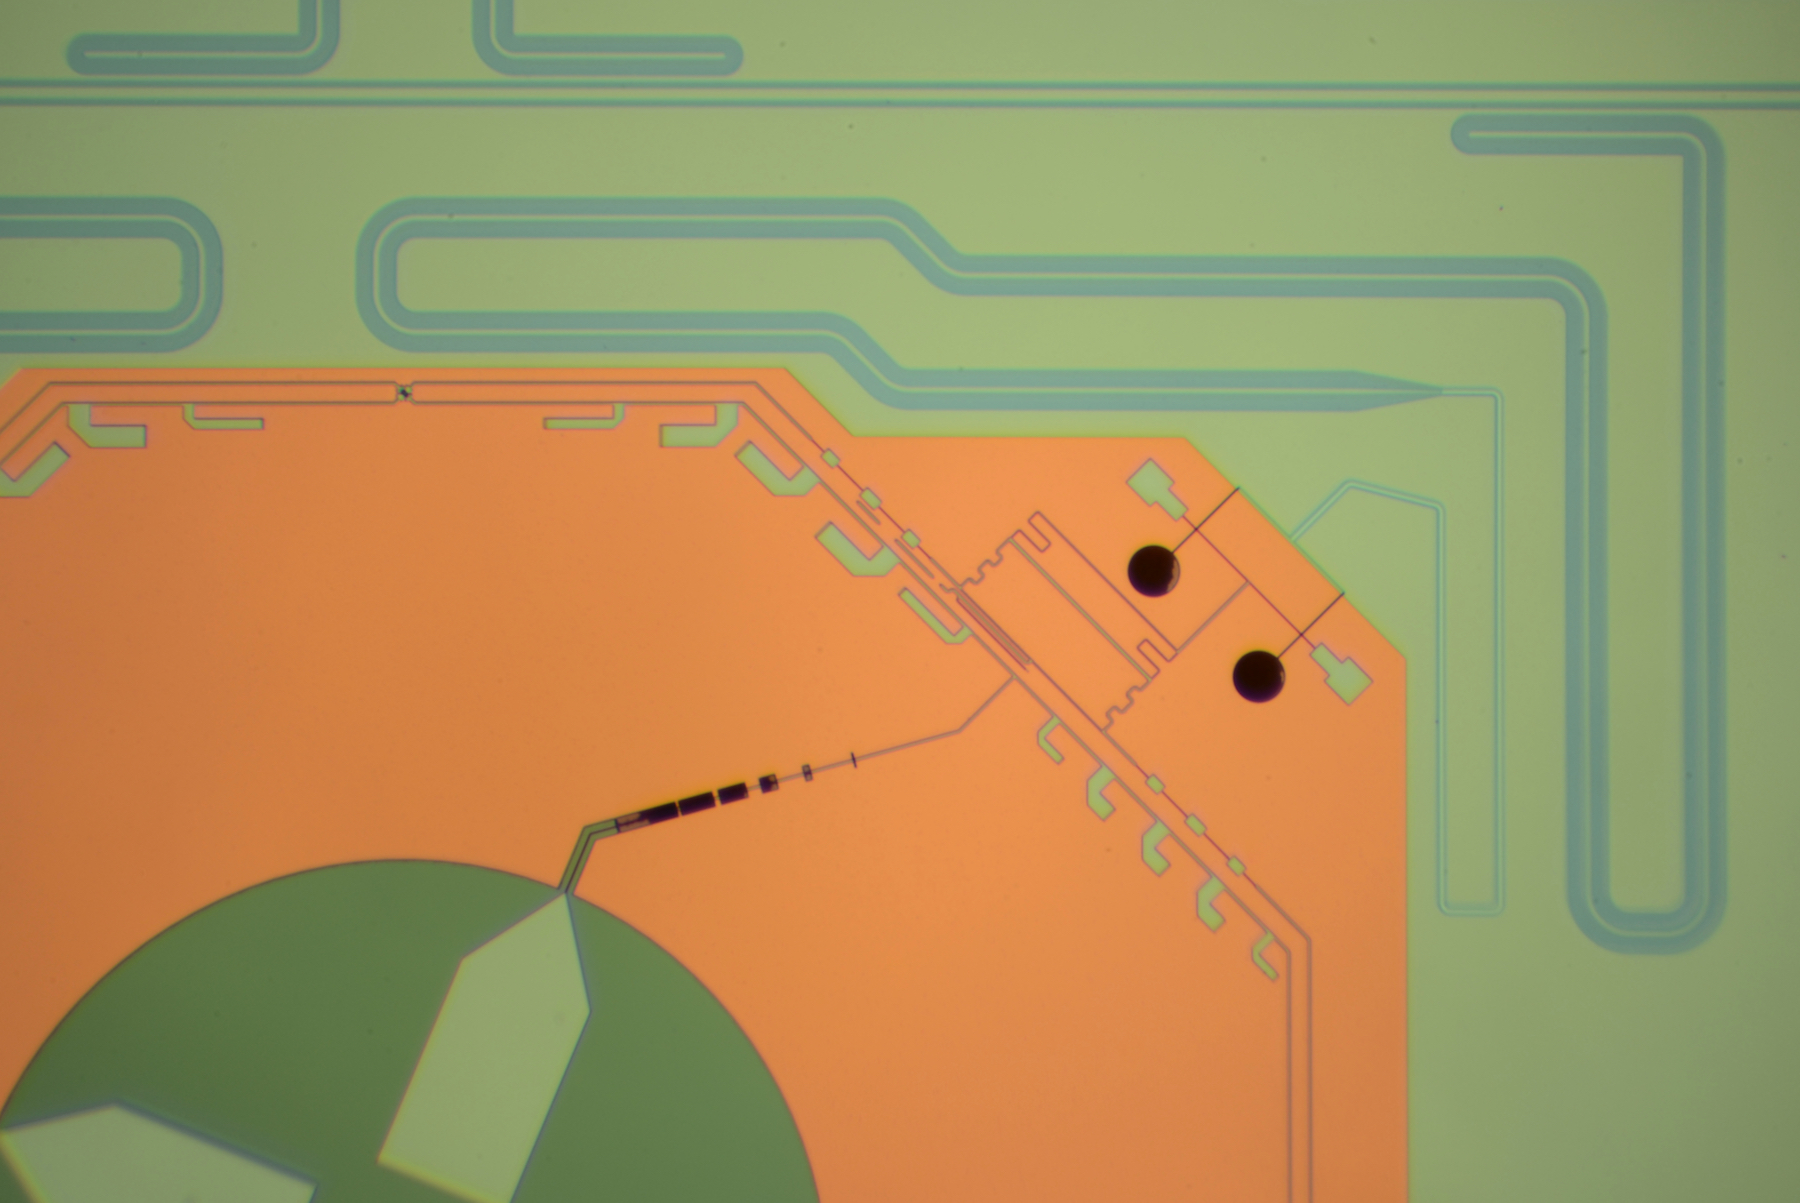
\includegraphics[width=0.8\textwidth]{multichroic/mkidarray01-0101_photo_one_resonator.jpg}
\caption[MKIDArray01-0101: a photograph of one resonator.]
{
MKIDArray01-0101: a photograph of one resonator, showing the area available in one corner of a pixel.
The ground plane appears green, and the exposed silicon is gray.
The orange structure is silicon nitride that is used for the microstrip circuitry and is removed from around the KIDs.
The horizontal transmission line that crosses the photograph is the feedline.
The area below the photo border is occupied by another resonator in the same pixel, and the area to the right of the photo border is occupied by a resonator in the adjacent pixel.
Photo courtesy of Brad Johnson.
}
\label{fig:mkidarray01-0101_photo_one_resonator}
\end{figure}

Using input from the simulations, I drew and tested prototype CPW resonators in order to explore resonator designs and provide feedback to collaborators on fabrication issues such as film quality.
Figure~\ref{fig:multichroic_prototypes} shows a drawing of a chip with eight CPW resonators and a photograph of a small aluminum package I designed that containing a chip fabricated by our colleagues at Stanford University. % Sherry Cho and Dale Li 
All of the prototype resonators consisted of either one or two films on high-resistivity, float-zone silicon substrates, so they involved a small number of fabrication steps.

\begin{figure}[htb]
\centering
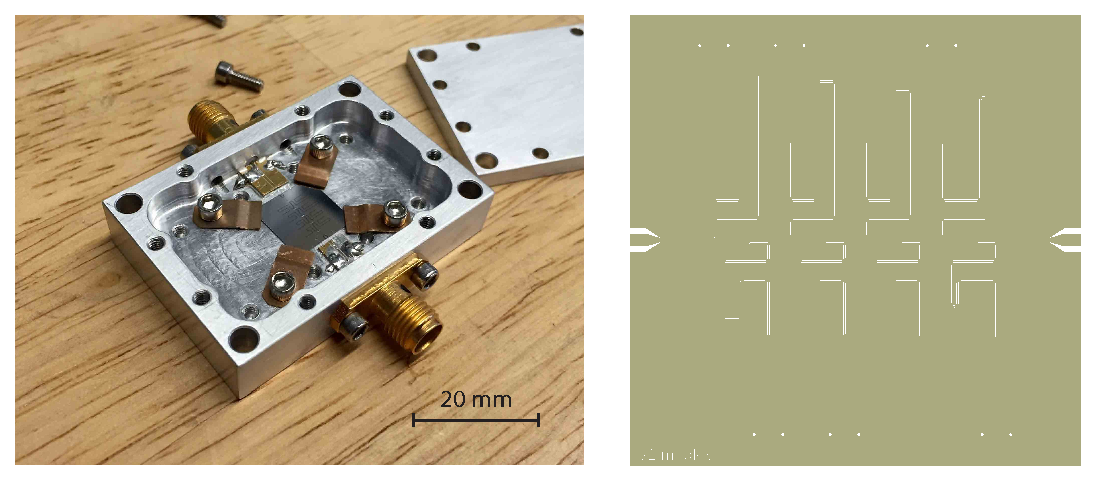
\includegraphics[width=\textwidth]{multichroic/multichroic_prototypes.pdf}
\caption[A photograph and a drawing of a chip with eight prototype resonators.]
{
\textbf{(Left)}
A photograph of a chip with eight prototype CPW KIDs in a small aluminum package designed for dark testing.
\textbf{(Right)}
A drawing of an eight-resonator chip that contains four different resonator types that are designed to test different aspects of the design.
The tan area is niobium, the red area is aluminum, and the white areas are exposed substrate.
This figure was published in \textcite{Johnson2016SPIE}.
}
\label{fig:multichroic_prototypes}
\end{figure}

Some tests were performed in a cryostat that had no magnetic shielding, and early generations of prototype resonators had high internal loss.
After we recognized that the magnetic shielding was insufficient, we obtained sheets of a nickel-iron-cobalt alloy (similar to mu-metal) and formed them by hand into a small box with end caps.
We tested the next generation of all-niobium resonators inside this box.
While this material had not been validated for cryogenic use, we obtained much lower internal loss
$\loss_\internal \sim \num{2.5e-6} = 1 / (\num{4e5})$.
This result suggested that vortices had caused some of the loss in previous generations of resonators.

The simulations and prototype resonators included the slot structures on the ground plane layer of the MS-to-CPW coupler, which are visible in Figure~\ref{fig:multichroic_prototypes}.
Our conclusion from simulations and measurements was that the slotline sections, which are electrically short at the KID resonance frequencies, did not have a significant effect on the resonators.

The initial KID design called for the active region to consist of a \SI{40}{nm} strip of aluminum deposited on top of the \SI{200}{nm} niobium ground plane layer.
To ensure continuity of the aluminum, the plan was to use a niobium etch that produced a sloped transition between the top of the niobium and the exposed silicon.
Due to difficulties in developing a high-yield fabrication process for the aluminum-over-niobium design, we explored a new fabrication process.
This niobium-over-aluminum process involved first depositing the aluminum followed immediately by the niobium without breaking vacuum, to avoid oxide formation.
Then, the niobium was etched from the CPW gaps and from the active region.
Finally, the aluminum was etched from the CPW gaps.
The resulting structure consists of a niobium-aluminum bilayer everywhere except for the active region, which is only aluminum.
Despite the continuity of the aluminum, the gap energy in the aluminum underneath the niobium should be significantly elevated due to the proximity effect, and the structure is expected to trap quasiparticles in the active region.
Prototype niobium-over-aluminum resonators had high loss under dark conditions, typically
$\num{2.5e-5} < \loss_\internal < \num{2e-4}$,
corresponding to 
$\num{40000} > \qf_\internal > \num{5000}$.
We have not yet been able to determine whether this loss is due to vortices, to the fabrication process, or to effects inherent to the bilayer.
The two 23-pixel wafers described below were fabricated with niobium-over-aluminum bilayers.


\section{The 23-pixel design}
\label{sec:multichroic.23-pixel}

Our collaborators at Stanford University used the structures resulting from the electromagnetic simulations and arranged them to produce a layout for the millimeter-wave circuitry. % Sherry Cho, Dale Li, and Yanru Song 
Using input from my simulations and from the prototype resonators, I designed 92 KID resonators and a feedline to add to this layout.
Figure~\ref{fig:multichroic_23-pixel_layout} is a drawing of the resulting 23-pixel design.

\begin{figure}[htb]
\centering
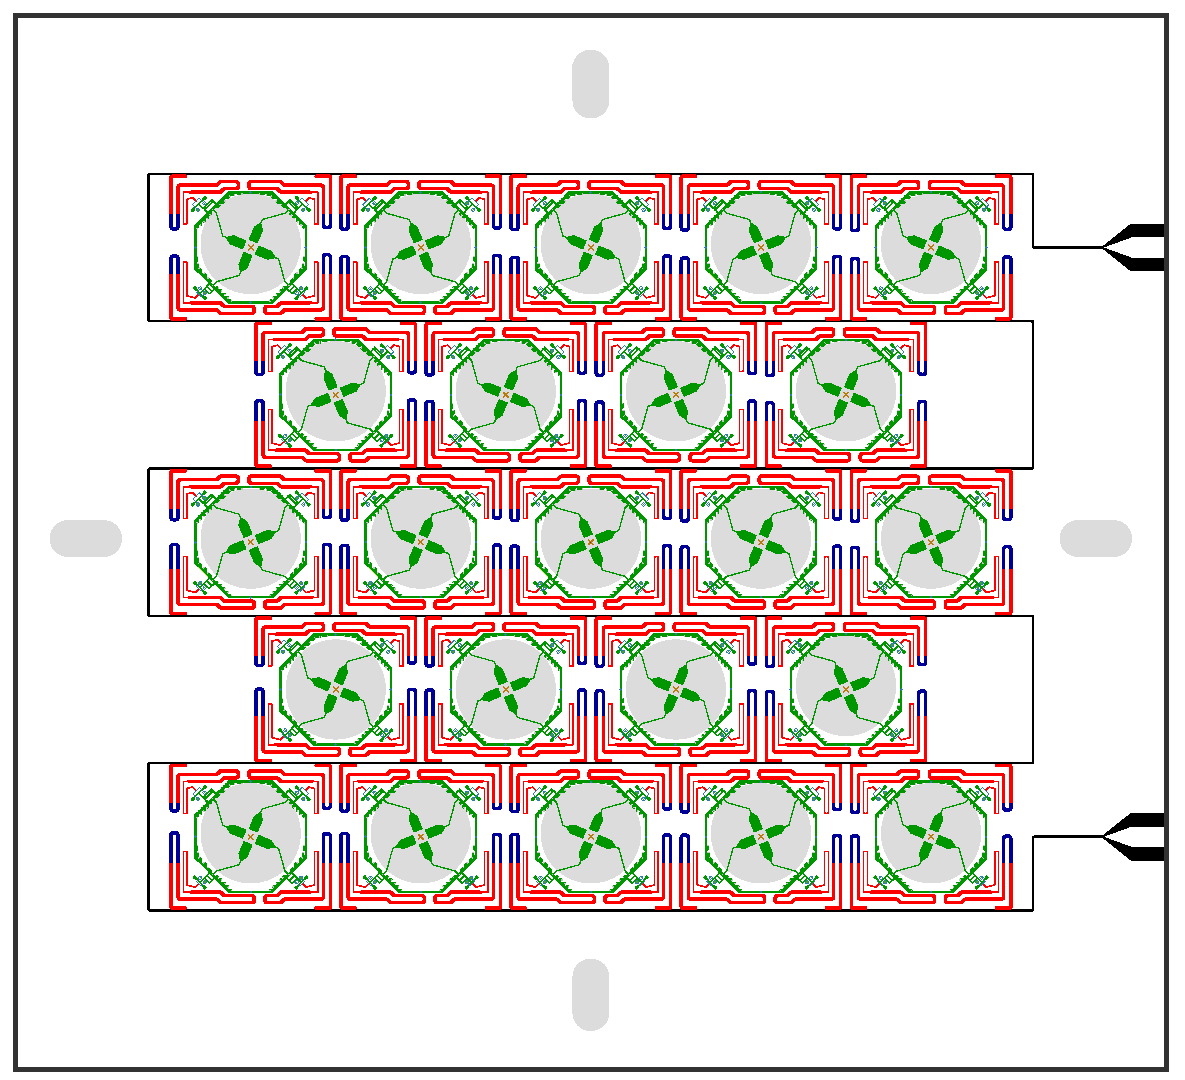
\includegraphics[width=0.7\textwidth]{multichroic/multichroic_23-pixel_layout.pdf}
\caption[A drawing of the multichroic 23-pixel array.]
{
A drawing of the multichroic 23-pixel array.
The pixel centers are separated by \SI{4.8}{mm} and the chip is approximately \SI{30}{mm} on each side.
There are two pixel polarization axes that differ by \SI{45}{\degree} and alternate along the rows.
The feedline meanders between the pixels and is connected to external transmission lines using the bond pads at right.
The four gray ovals are alignment slots that are etched in the silicon.
Precisely machined bosses on the holder protrude into these slots and align the chip to within about \SI{10}{\micro\meter}, while allowing for differential thermal contraction between the silicon and aluminum.
%See Appendix~\ref{chp:hardware}.
}
\label{fig:multichroic_23-pixel_layout}
\end{figure}

Each KID on a given feedline requires a unique resonance frequency, so some part of each KID must be unique.
The chips containing eight prototype resonators had a square footprint \SI{10}{mm} on a side, which could be flashed using a single photomask.
In order to fabricate the much larger 23-pixel (92-resonator) array using a reasonable number of photomasks, we fixed the lengths of the active regions and set each resonance frequency by tuning the length of the inactive region using a ``trombone slide'' structure.
In both Figure~\ref{fig:multichroic_mkid_coupling_v3} and Figure~\ref{fig:multichroic_23-pixel_layout}, the KIDs are drawn in both red and blue.
The red areas are identical between all pixels, while the blue areas vary between pixels because the trombone slide overlaps the fixed region by different amounts and produces a different total length for each KID.

The geometry of the active CPW section was determined based on both the simulations of the MS-to-CPW coupling and on simulations that indicated that nearly all of the millimeter wave light would be absorbed over a length of about \SI{2}{mm}.
The aluminum center strip in the active region is \SI{4}{\micro\meter} wide, and the gaps to the niobium-over aluminum ground plane are \SI{5}{\micro\meter} wide.
The active region is \SI{2.1}{mm} long for the \SI{150}{GHz} detectors and is \SI{2.7}{mm} long for the \SI{235}{GHz} detectors.
The aluminum strip is longer for the \SI{235}{GHz} detectors because we anticipate they will receive more power from the sky, so their volume needs to be larger to maintain equal dissipation.
The geometry of the inactive section, made from the niobium-over-aluminum bilayer, has a length range of \SIrange{8.8}{10.4}{mm}.
The end of the resonator near the readout transmission line supports the largest electric fields and is therefore most susceptible to TLS effects~\autocite{Gao2008aAPL, Gao2008bAPL,Zmuidzinas2012ARCMP}.
To reduce these effects, the inactive center strip is \SI{10}{\micro\meter} wide and the gaps to the ground plane are \SI{30}{\micro\meter} wide.
The geometry of the elbow coupler that runs along the transmission line is the same as the rest of the inactive CPW.
The feedline is CPW with a \SI{20}{\micro\meter} center strip and \SI{12}{\micro\meter} gaps to the ground plane.
It is designed to match the \SI{50}{\Omega} impedance of the boards that carry signals to and from the coaxial connectors and the chip.

The exact lengths were calculated for each resonator assuming the effective dielectric constant discussed above and an effective kinetic inductance fraction of 20\% for all resonators, which is an approximation.
Because the \SI{235}{GHz} detectors have longer active sections, their inactive sections are proportionally longer, and they have lower resonance frequencies than the \SI{150}{GHz} detectors.
The low-frequency \SI{235}{GHz} detectors are in the lower left of each pixel, and their resonance frequencies span \SIrange{2542}{2634}{MHz}.
The high-frequency \SI{235}{GHz} detectors are in the lower right of each pixel, and their resonance frequencies span \SIrange{2664}{2756}{MHz}.
The low-frequency \SI{150}{GHz} detectors are in the upper right of each pixel, and their resonance frequencies span \SIrange{2786}{2878}{MHz}.
The high-frequency \SI{150}{GHz} detectors are in the upper left of each pixel, and their resonance frequencies span \SIrange{2908}{3000}{GHz}.
The bands were separated by \SI{30}{MHz} in order to reduce frequency collisions.
The total bandwidth of about \SI{460}{MHz} allows all 92 resonators in the array to be read out simultaneously using our heterodyne system if the local oscillator frequency is placed between the two middle bands.

\begin{table}[htb]
\centering
\footnotesize
\caption[The stack-up for the first multichroic detector array on a SOI wafer.]
{
The stack-up for the first multichroic detector array on a SOI wafer.
The direction of light propagation is from the bottom of the table to the top.
Because the thick silicon handle wafer and silicon oxide layer are etched away from under the OMTs, the light first encounters the thin silicon device layer.
HTO: hot thermal oxide.
}
\renewcommand{\arraystretch}{1.2}
\begin{tabular}{c d{2} l}
\toprule
Material & \mathrm{Thickness} / \si{\micro m} & Notes \\
\midrule
Al & \mathrm{bulk} & lid with back-shorts \\
vacuum & \mathrm{varies} & from metal on wafer to package bulk metal \\
\midrule
Au & 0.1 & \SI{180}{\degree} tee termination and heat sink wirebond pads \\
Nb & 0.4 & microstrip: filters, hybrids, coupler; feedline cross-overs \\
SiN$_x$ & 0.35 & not present above the resonators or feedline \\
Nb & 0.2 & ground plane: resonators, feedline, OMTs \\
Al & 0.04 & ground plane and KID active region \\
\midrule
Si (intrinsic $\langle 100 \rangle$) & 5 & resistivity $>\SI{e4}{\ohm.cm}$, float-zone; thickness $\pm \SI{0.5}{\micro m}$ \\
SiO$_2$ (wet HTO) & 0.5 & thickness $\pm 5\%$ \\
Si (P / boron $\langle 100 \rangle$) & 350 & resistivity \SIrange{1}{10}{\ohm.cm}; thickness $\pm \SI{5}{\micro m}$ \\
\hline
Al & \mathrm{bulk} & holder with feedhorns and circular waveguides \\
\bottomrule
\end{tabular}
\label{tab:multichroic_stack-up}
\end{table}


\section{Fabrication}
\label{sec:multichroic.fabrication}

All of the arrays were fabricated by our collaborators at Stanford University.
The first 23-pixel KID array was fabricated on SOI wafers \SI{100}{mm} in diameter.
Each SOI wafer consists of a \SI{5}{\micro\meter} thick float-zone silicon (> \SI{10}{k\Omega.cm} resistivity) device layer and a \SI{350}{\micro\meter} thick silicon handle wafer held together by a \SI{0.5}{\micro\meter} thick buried oxide layer.
An aluminum-niobium bilayer is first deposited on the device layer.
The aluminum is \SI{40}{nm} thick and the niobium is \SI{200}{nm} thick.
This bilayer forms the ground plane, and is patterned to produce the OMTs, some millimeter-wave circuitry, the coupler slotlines and KIDs, and the feedline.
A \SI{350}{nm} thick film of silicon nitride (SiN$_x$) is deposited on top of the bilayer, followed by a \SI{400}{nm} thick niobium film.
The silicon nitride serves as the electrically insulating dielectric material in the microstrip, and the niobium film is patterned to form the microstrip circuit that includes the band-pass filters and the \SI{180}{\degree} hybrids.
Our design uses cross-unders~\autocite{Duff2016JLTP} in the microstrip circuit rather than cross-overs, which decreases the number of required fabrication steps.
A gold film is deposited and patterned on top of the silicon nitride to construct the termination resistor at the sum port of the \SI{180}{\degree} hybrid.
The silicon nitride is removed near the KIDs to reduce loss and two-level system noise.
The niobium is removed from the approximately \SI{2}{mm} long sensing section of the center line of the KIDs, leaving only the aluminum.
To form the membrane and alignment slots, the thick silicon handle wafer is removed using deep reactive ion etching (DRIE), and the buried oxide layer is then removed using hydrogen fluoride (HF) vapor.
To reduce TLS noise and loss, these dielectrics are also removed from underneath the high-field section of the KIDs.
Table~\ref{tab:multichroic_stack-up} summarizes the fabrication stack-up.


\section{MKIDArray01-0101: a 23-pixel array on intrinsic silicon}
\label{sec:multichroic.mkidarray01}

In order to test fabrication steps and the resonator design, we produced an engineering array on a monolithic \SI{500}{\micro\meter} thick high-resistivity, float-zone silicon wafer.
This engineering wafer, which we called MKIDArray01, was not optimized for millimeter-wave coupling because the substrate was too thick.
I tested chip 0101 from this wafer in a simplified version of the aluminum horn package with no horns, chokes, or backshorts.
Figure~\ref{fig:mkidarray01_in_dark_and_horn} shows a photograph of this array in a dark holder, as well as a holder with conical horns that was used later on for optical testing.
The package was enclosed in a box made from magnetic shielding material.

\begin{figure}[htb]
\centering
\includegraphics[width=\textwidth]{multichroic/mkidarray01_in_dark_and_horn.pdf}
\caption[Photographs of the holder, showing the conical horns, and of MKIDArray01-0101 in a dark holder.]
{
Photographs of the holder, showing the conical horns, and of MKIDArray01-0101 in a dark holder.
}
\label{fig:mkidarray01_in_dark_and_horn}
\end{figure}

Figure~\ref{fig:mkidarray01_full_s21_sweep} shows the result of sweeping readout tones from \SIrange{1.8}{4.0}{GHz} and recording the complex forward scattering parameter $\forwardscattering$.
All 92 designed resonances seemed to be present, along with some additional resonances that did not respond much to temperature changes and thus could be box modes or resonances involving the ground plane.
The KID resonances appeared slightly above the nominal resonance frequencies, indicating that the effective kinetic inductance fractions were slightly less than the 20\% estimate used to calculate the resonator lengths.

The scatter in the measured resonance frequencies, apparent in the frequency sweep, is due to a known effect.
The elbow coupler radiates onto the feedline both the quasi-TEM mode, in which the ground planes have the same voltage, and a so-called slotline mode, in which the ground plane voltages are different.
The slotline mode can be trapped on the chip and develop standing waves, which affect both the coupling strength and the location of the resonance frequency.
This effect can be mitigated by electrically connecting the ground planes of the CPW~\autocite{Mates2011, Yates2014JLTP}.
We designed cross-overs to address this issue, but did not include them in the photomask set used for the wafers described in this thesis because the fabrication process was not yet developed.

\begin{figure}[htb]
\centering
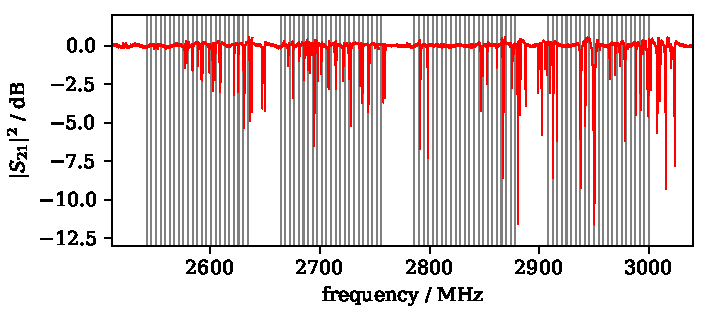
\includegraphics[width=\textwidth]{multichroic/mkidarray01_full_s21_sweep.pdf}
\caption[MKIDArray01-0101: a wide frequency sweep showing many resonance dips.]
{
MKIDArray01-0101: a wide frequency sweep showing many resonance dips.
The vertical gray lines show the nominal resonance frequencies.
}
\label{fig:mkidarray01_full_s21_sweep}
\end{figure}

We fit the resonances identified in the frequency sweep to the model given in Section~\ref{sec:theory.resonator} to determine the internal and coupling quality factors for many of the resonators on the array.
Figure~\ref{fig:mkidarray01_histogram_Qi_Qc} shows a histogram of the result.
The coupling quality factors show wide scatter that is expected in the absence of cross-overs.
The internal quality factors are clustered just below
$\qf_\internal \sim \num{20000}$,
corresponding to
$\loss_\internal \sim \num{5e-5}$.
Although the magnetic shielding has improved, the loss values are similar to those obtained in the prototype niobium-over-aluminum resonators, suggesting that vortices are not dominating the loss.
The internal loss was nearly independent of readout power, so TLS loss is unlikely to be significant. 

\begin{figure}[htb]
\centering
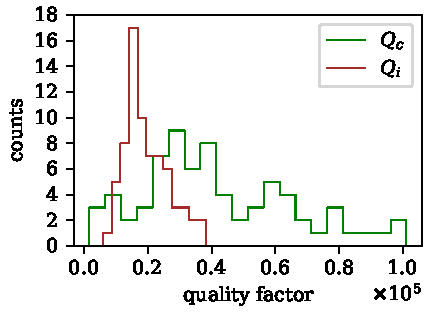
\includegraphics[width=0.5\textwidth]{multichroic/mkidarray01_histogram_Qi_Qc.pdf}
\caption[MKIDArray01-0101: a histogram of resonator quality factors.]
{
MKIDArray01-0101: a histogram of resonator quality factors.
}
\label{fig:mkidarray01_histogram_Qi_Qc}
\end{figure}

The response of seven resonators to varying bath temperature is shown in Figure~\ref{fig:mkidarray01_seven_s_and_i_vs_temperature}.
The central five resonators respond qualitatively as expected for resonators containing aluminum.
The leftmost and rightmost resonators, which seem not to be KIDs, barely respond to the temperature change.

\begin{figure}[htb]
\centering
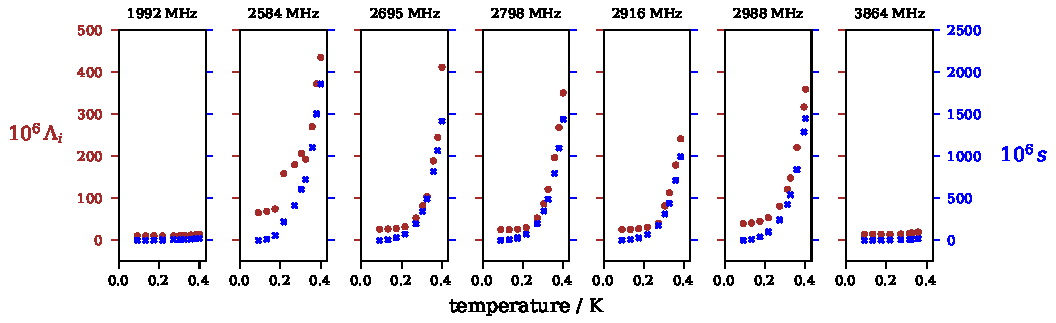
\includegraphics[width=\textwidth]{multichroic/mkidarray01_seven_s_and_i_vs_temperature.pdf}
\caption[MKIDArray01-0101: response to changing bath temperature for seven resonators.]
{
MKIDArray01-0101: response to changing bath temperature for seven resonators.
The left axes all share the same limits, and show internal loss $\loss_\internal$.
The right axes all share the same limits, which are much larger, and show the fractional frequency shift
$\shift(\temperature)$
from the maximum measured resonance frequency $\freadout_\resonator^\mathrm{max}$.
}
\label{fig:mkidarray01_seven_s_and_i_vs_temperature}
\end{figure}

The critical temperature was measured to be, using the through transmission on the bilayer feedline, $\tc = \SI{8.3}{K}$, somewhat reduced from the value of \SI{9.3}{K} for bulk niobium.
The resonators become too lossy to measure as the chip temperature approaches the critical temperature of aluminum, so the aluminum film transition temperature is unknown.


\section{MKIDArray02-0001: a 23-pixel array on SOI}
\label{sec:multichroic.mkidarray02}

\begin{figure}[htb]
\centering
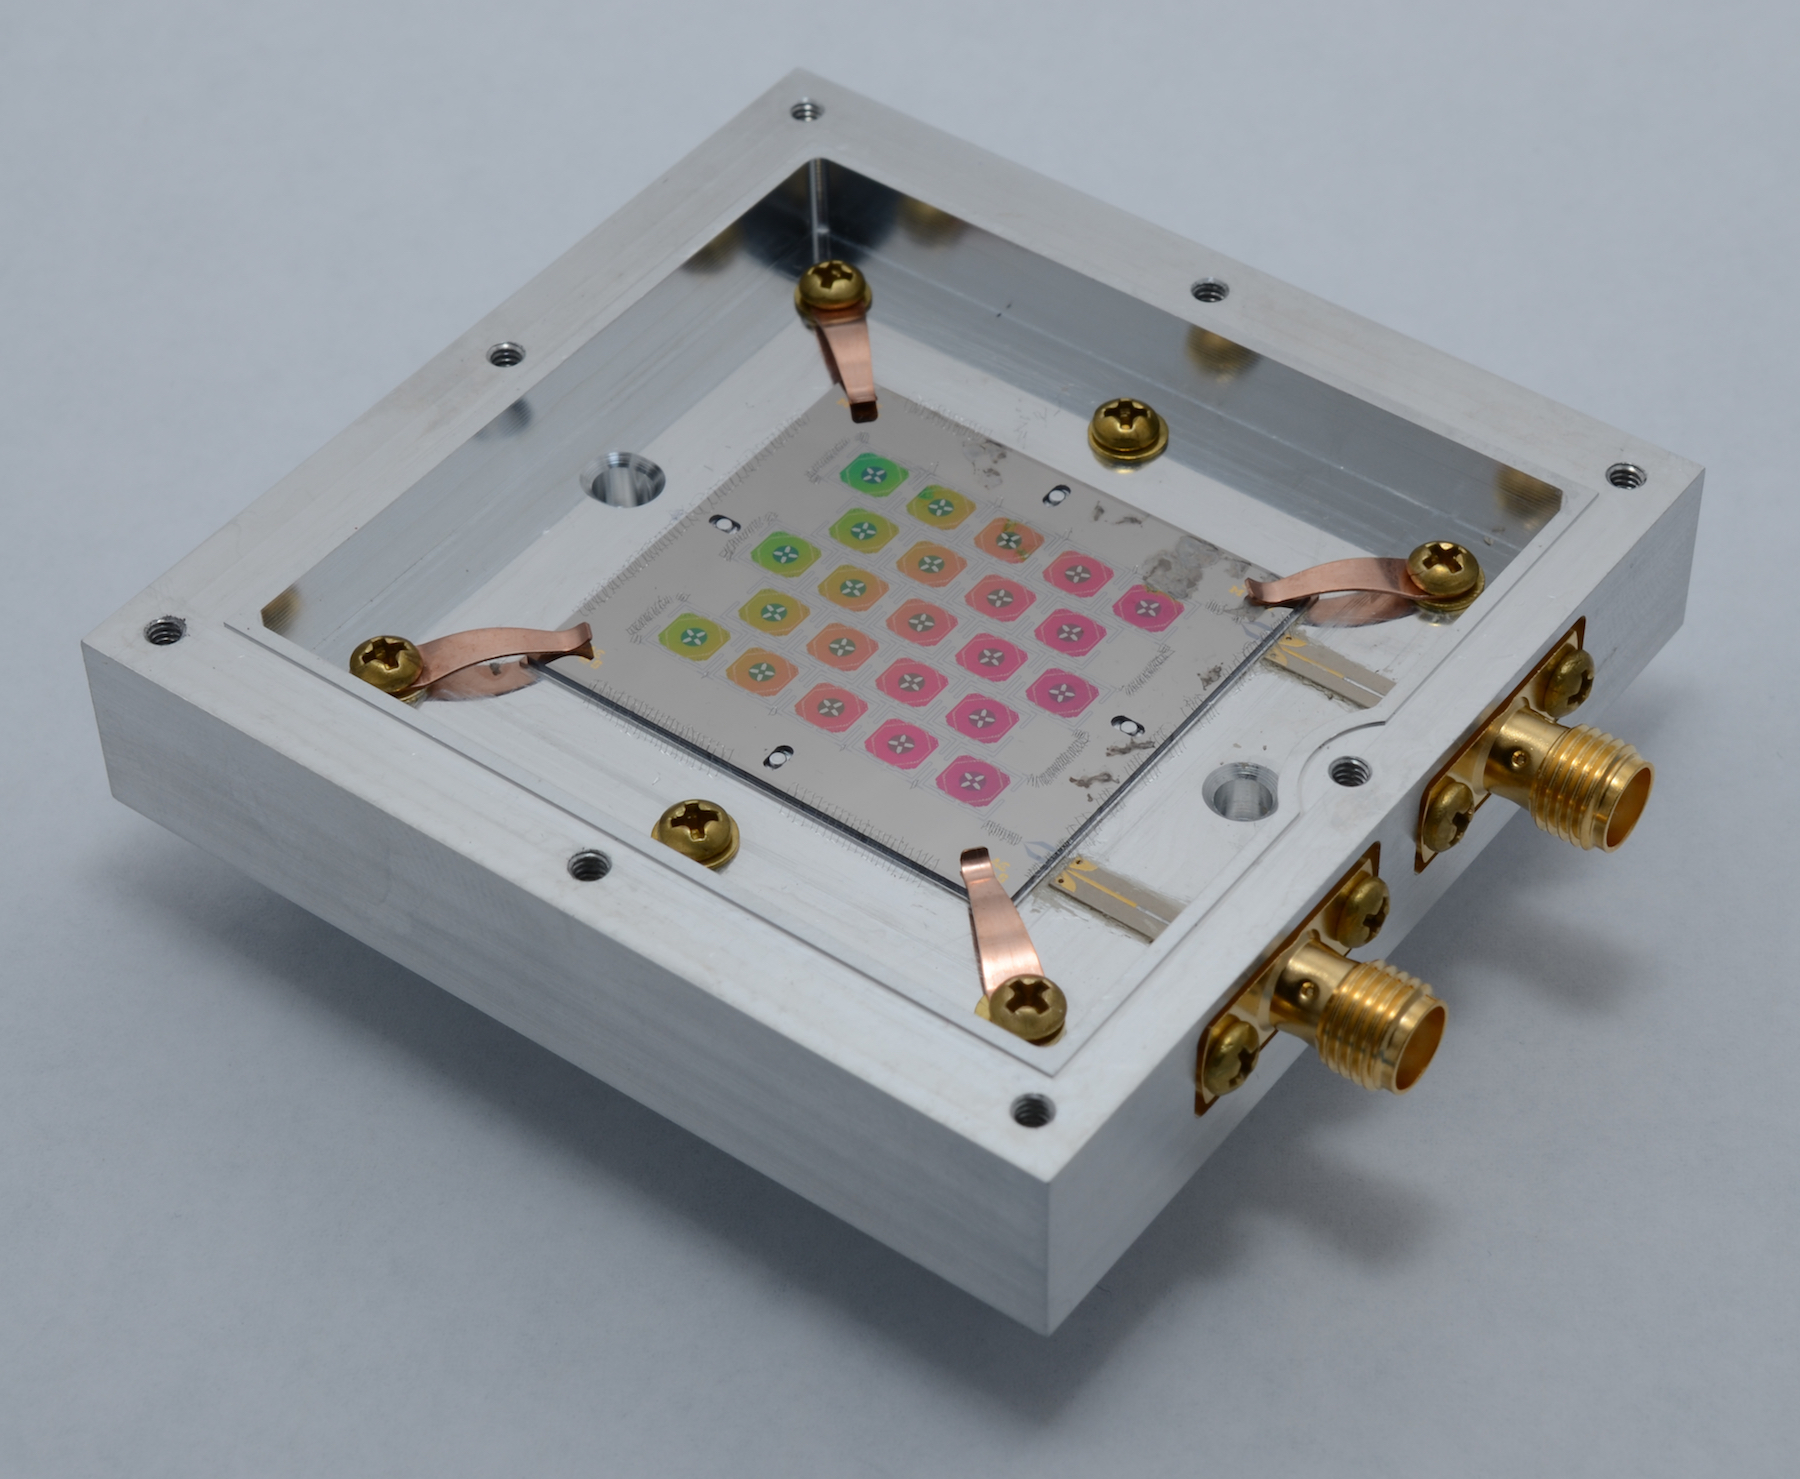
\includegraphics[width=0.5\textwidth]{multichroic/MKIDArray02-0001_in_package.jpg}
\caption[MKIDArray02-0001: a photograph of the first 23-pixel chip on a silicon-on-insulator wafer.]
{
MKIDArray02-0001: a photograph of the first 23-pixel chip on a silicon-on-insulator wafer in a package I designed for optical testing.
Photo courtesy of Brad Johnson.
}
\label{fig:MKIDArray02-0001_photo}
\end{figure}

This wafer, which we called MKIDArray02, was the first to be fabricated using SOI.
I tested one 23-pixel chip from this wafer, number 0001.
The dielectrics were removed from underneath the elbow couplers, which is the area of highest electric field.
Figure~\ref{fig:starcryo_cryostat_with_hwp} is a photograph of the cryostat that shows the experimental configuration and the optical components I used to illuminate the detectors.
I used both the Eccosorb black body source and the electronic millimeter-wave source for these first optical tests.
Figure~\ref{fig:mkidarray02_wide_sweep_180_mK_real_and_fake} shows wide frequency sweeps at two temperatures, which were used to distinguish between KIDs and spurious resonances.
I was able to identify 66 of the 92 expected KID resonances, as well as a number of additional resonances that do not seem to be KIDs.

\begin{figure}[htb]
\centering
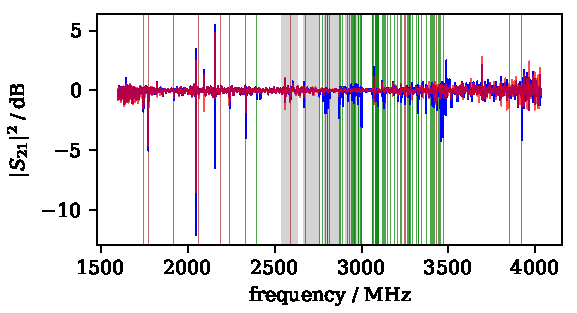
\includegraphics[width=0.8\textwidth]{multichroic/mkidarray02_wide_sweep_180_mK_real_and_fake.pdf}
\caption[MKIDArray02-0001: wide frequency sweeps at two temperatures.]
{
MKIDArray02-0001: wide frequency sweeps at two temperatures.
The red data points were acquired with the package temperature at \SI{0.2}{K}, while the blue data points were acquired at \SI{0.8}{K}.
Aluminum is relatively lossy at the higher temperature, so resonances that produce a transmission dip at this temperature must not be KIDs.
The gray vertical lines show the nominal resonance frequencies.
The brown vertical lines show the frequencies of spurious resonances that remained at the higher temperature.
The green vertical lines show the frequencies of resonances that vanished at the higher temperature and are thus likely to be KIDs.
}
\label{fig:mkidarray02_wide_sweep_180_mK_real_and_fake}
\end{figure}

I measured in detail a subset of 34 resonances, several of which subsequently turned out not to be KIDs.
Data from these resonances is shown in Figures~\ref{fig:mkidarray02_all_scans_Qi_and_Qc_vs_frequency},~\ref{fig:mkidarray02_all_bath_temperature_response},~\ref{fig:mkidarray02_loss_i_and_loss_c_versus_readout_power}, and~\ref{fig:mkidarray02_all_eccosorb_response}.
In some cases, data cuts reduced the number of analyzed resonators below 34.

\begin{figure}[htb]
\centering
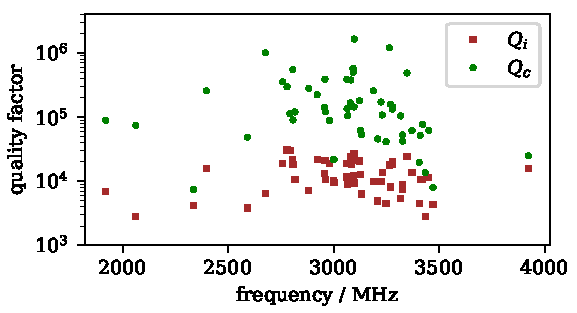
\includegraphics[width=0.7\textwidth]{multichroic/mkidarray02_all_scans_Qi_and_Qc_vs_frequency.pdf}
\caption[MKIDArray02-0001: $\qf_\internal$ and $\qf_\coupling$ versus frequency.]
{
MKIDArray02-0001: $\qf_\internal$ and $\qf_\coupling$ versus frequency.
}
\label{fig:mkidarray02_all_scans_Qi_and_Qc_vs_frequency}
\end{figure}

Figure~\ref{fig:mkidarray02_all_scans_Qi_and_Qc_vs_frequency} shows the quality factors extracted from fitting this group of resonances at a bath temperature of \SI{0.19}{K}, which was used for most data collection.
(Due to a cryogenic problem, I used a somewhat higher bath temperature than normal.)
Many of the the other resonances were very shallow or were difficult to analyze due to frequency collisions.
The internal quality factors are similar to those found on the engineering array.
The coupling quality factors are several times higher than on the engineering array, probably because the removal of the dielectrics under the elbow coupler reduces the capacitance between it and the feedline.
The coupling strength can easily be increased by lengthening the section of elbow coupler parallel to the feedline or by moving it closer to the feedline.
The combination of low coupling strength and high internal loss makes the resonances wide and shallow, mostly less than \SI{1}{dB} deep.
Such resonances are difficult to distinguish from the ripple in the background transmission.
It is thus likely that more resonances are present than I was able to identify.

\begin{figure}[htb]
\centering
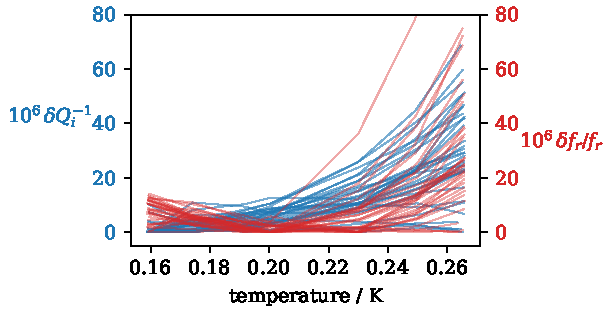
\includegraphics[width=0.8\textwidth]{multichroic/mkidarray02_all_bath_temperature_response.pdf}
\caption[MKIDArray02-0001: response to changing bath temperature.]
{
MKIDArray02-0001: response to changing bath temperature.
The minimum value of the internal loss for each detector has been subtracted, and the left axis shows the change in loss.
The right axis shows fractional frequency shift $\shift$.
}
\label{fig:mkidarray02_all_bath_temperature_response}
\end{figure}

Measurements of the response of the same 34 resonators to changing bath temperature are shown in Figure~\ref{fig:mkidarray02_all_bath_temperature_response}.
At high temperatures, both $\loss_\internal$ and $\shift$ increase with increasing temperature, as expected.
The low-temperature increase in $\shift$ as the temperature decreases is a signature of TLS effects, and is sometimes called ``back-bending.''

\begin{figure}[htb]
\centering
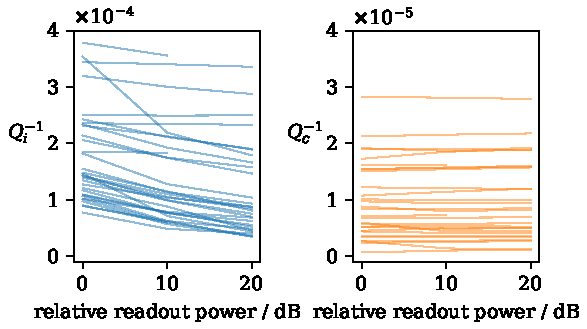
\includegraphics[width=0.8\textwidth]{multichroic/mkidarray02_loss_i_and_loss_c_versus_readout_power.pdf}
\caption[MKIDArray02-0001: response to changing readout power.]
{
MKIDArray02-0001: response to changing readout power.
The left plot shows internal loss, and the right plot shows coupling loss.
}
\label{fig:mkidarray02_loss_i_and_loss_c_versus_readout_power}
\end{figure}

Figure~\ref{fig:mkidarray02_loss_i_and_loss_c_versus_readout_power} shows the response of the internal and coupling loss to changing readout power.
The observed decrease in $\loss_\internal$ with increasing readout power is a signature of TLS loss.
This occurs because the TLS become saturated~\autocite{Zmuidzinas2012ARCMP}.
\todo[inline]{Backbending in Budoyo2016PRB?}
%However, similar behavior has also been attributed to nonequilibrium effects caused by the readout~\autocite{Budoyo2016PRB}.
Because the internal loss of the resonators fabricated on intrinsic silicon was nearly independent of readout power, the buried oxide layer in this array is the likely culprit.
As usual, the coupling strength $\loss_\coupling$ is independent of readout power.

\begin{figure}[htb]
\centering
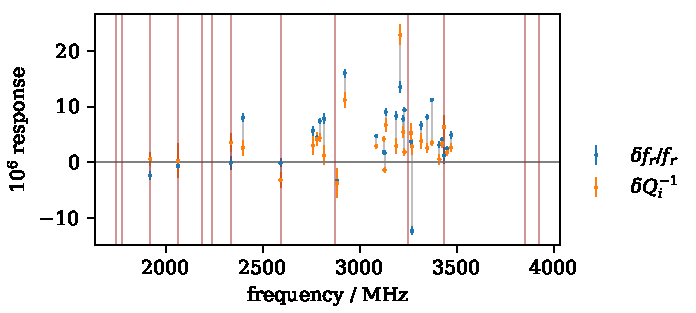
\includegraphics[width=0.8\textwidth]{multichroic/mkidarray02_all_eccosorb_response.pdf}
\caption[MKIDArray02-0001: response to changing black body temperature.]
{
MKIDArray02-0001: response of 29 resonators to changing black body temperature.

}
\label{fig:mkidarray02_all_eccosorb_response}
\end{figure}

I tested the response of the same set of detectors to a change in the temperature of a black body load.
This load is the slab of Eccosorb, a material that is black at millimeter wavelengths, that is shown in Figure~\ref{fig:starcryo_cryostat_with_hwp}.
The thickness is such that the slab is nearly opaque, and the transverse extent is sufficient to fill the detector feed horn beams.
The slab has an anti-reflection coating of etched Teflon.
I measured the resonators with the black body at \SI{3.3}{K}, the base temperature of the slab, and at \SI{5.0}{K}, heating the slab using a resistor attached to the slab support structure.
The changes in the internal loss and coupling loss are shown in Figure~\ref{fig:mkidarray02_all_eccosorb_response}.
The brown vertical lines mark the locations of the spurious resonances that were identified later.
These resonances respond either anomalously or not at all the the black body.
The identified KID resonances mostly shift similarly, with the fractional frequency shift $\shift = \delta \freadout_\resonator / \freadout_\resonator$ somewhat higher than the internal loss shift $\delta \loss_\internal$, as expected.
The fractional frequency shift is about 4 parts per million per degree kelvin.

% Chosen one
I chose one resonator to analyze in more detail.
This resonator has a resonance frequency 
$\freadout_\resonator = \SI{3410}{MHz}$
and it is thus likely to be a \SI{150}{GHz} detector.
The internal loss and coupling loss are
\begin{align}
\loss_\internal &= \num{8.14e-5} = 1 / (\num{1.23e4}) \\
\loss_\coupling &= \num{1.92e-5} = 1 / (\num{5.22e4}).
\end{align}
This internal loss is typical for the array, while the coupling loss is lower than average, which makes the resonance deeper and easier to measure.
The resonator bandwidth is
\begin{equation}
\faudio_\resonator
  =
  \freadout_\resonator (\loss_\internal + \loss_\coupling) / 2
  = 
  \SI{170}{kHz},
\end{equation}
which is higher than the Nyquist frequency of \SI{125}{kHz}.
The quasiparticle relaxation time was extracted under similar conditions from the fit in Figure~\ref{fig:mkidarray02_chosen_one_x_fold_fit}, and the  corresponding quasiparticle bandwidth is
$\faudio_\quasiparticle
  =
  1 / (2 \pi \qprelaxationtime)
  =
  \SI{920}{Hz}$.
Figure~\ref{fig:mkidarray02_chosen_one_di_and_s_versus_temperature} shows the response of this resonator to changing bath temperature.
The interpretation of the results is complicated by what appear to be TLS effects on both the internal loss and fractional frequency shift.

\begin{figure}[htb]
\centering
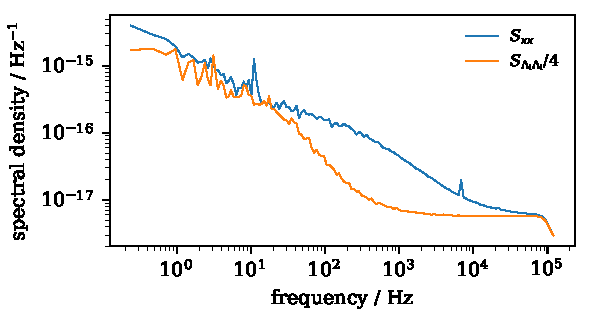
\includegraphics[width=0.8\textwidth]{multichroic/mkidarray02_chosen_one_noise_spectra.pdf}
\caption[MKIDArray02-0001: noise spectra for the \SI{3410}{MHz} resonator.]
{
MKIDArray02-0001: noise spectra for the \SI{3410}{MHz} resonator.
The plotted data are estimates of the power spectral densities of $\detuning(\time)$ and $\loss_\internal(\time)$ extracted from \SI{33}{s} of time-ordered data.
The normalization of the internal loss spectrum is chosen so that the amplifier noise has the same amplitude in both spectral densities.
The roll-off at the highest frequencies is due to an anti-aliasing filter in the readout firmware.
}
\label{fig:mkidarray02_chosen_one_noise_spectra}
\end{figure}

Figure~\ref{fig:mkidarray02_chosen_one_noise_spectra} shows noise data measured at a bath temperature of \SI{0.16}{K} with no optical illumination except for the black body at its \SI{3.3}{K} base temperature.
The spectral density $\spectraldensity_{\loss_\internal \loss_\internal}$ of the internal loss data falls off rapidly below \SI{100}{Hz} to the amplifier noise level and is then white out to the roll-off due to an anti-aliasing filter.
The temperature regulation was particularly unstable in this cooldown, and the stage temperature often fluctuated by up to \SI{1}{mK}, much more than normal.
Some of the noise is thus likely to be produced by changes in the thermal quasiparticle generation rate.
The excess seen in the spectral density $\spectraldensity_{\detuning \detuning}$ of the detuning data may be caused by TLS noise, but more tests would be required to determine the different contributions.

\begin{figure}[htb]
\centering
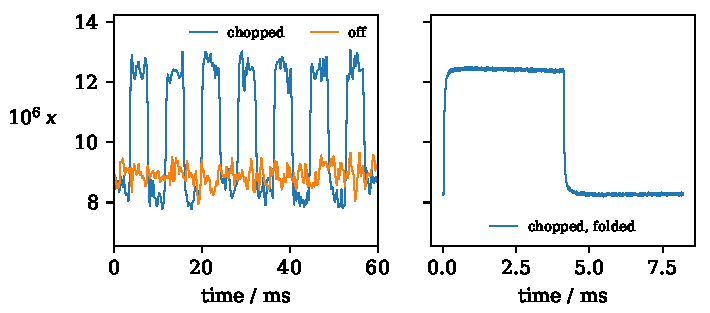
\includegraphics[width=\textwidth]{multichroic/mkidarray02_chosen_one_mmw_decimated_and_folded.pdf}
\caption[MKIDArray02-0001: decimated and folded time-ordered data for the \SI{3410}{MHz} resonator.]
{
\textbf{(Left)}
Time-ordered detuning data from the \SI{3410}{MHz} resonator.
One time series was taken with the millimeter-wave source off.
The other was taken with the signal chopped at \SI{122}{Hz} using a switch in the source.
Both time series have been decimated by a factor of 64 to remove high-frequency amplifier noise.
\textbf{(Right)}
The entire \SI{33}{s} time series of chopped data, part of which is shown in the left panel, has been folded down to a single period by averaging all samples that are separated by one period.
}
\label{fig:mkidarray02_chosen_one_mmw_decimated_and_folded}
\end{figure}

Figure~\ref{fig:mkidarray02_chosen_one_mmw_decimated_and_folded} shows the response of this detector to a chopped signal from the millimeter wave source described in Section~\ref{sec:sensitivity.measuring} and in Appendix~\ref{chp:hardware}.
The source was used in broadband mode, producing a chaotic  signal from \SIrange{140}{160}{GHz}.
Comparing the data to the black body response indicates that the source signal amplitude corresponds to about a \SI{1}{K} change.
The decay portion of the data shown in the right panel was used for the fit shown in Figure~\ref{fig:mkidarray02_chosen_one_x_fold_fit}.

\begin{figure}[htb]
\centering
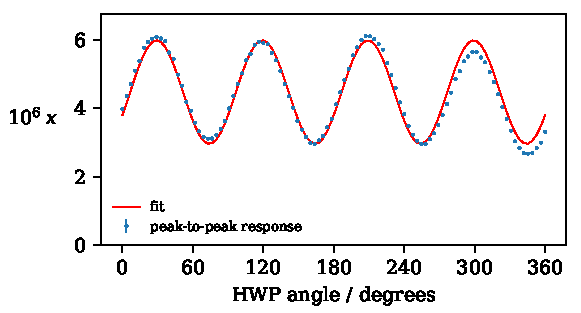
\includegraphics[width=0.8\textwidth]{multichroic/mkidarray02_chosen_one_fit_hwp.pdf}
\caption[MKIDArray02-0001: half-wave plate data for the \SI{3410}{MHz} resonator.]
{
MKIDArray02-0001: half-wave plate data for the \SI{3410}{MHz} resonator.
Each blue point is the peak-to-peak amplitude of the time-ordered detuning data at that HWP angle with the source chopped at \SI{122}{Hz}, with statistical error bars.
The amplitude was calculated from about \SI{1}{s} of time-ordered data that was folded to a single period of the chop signal, as in the right panel of Figure~\ref{fig:mkidarray02_chosen_one_mmw_decimated_and_folded}.
The red line is a fit to an offset sine with a period of one quarter HWP rotation, which is the expected modulation period.
}
\label{fig:mkidarray02_chosen_one_fit_hwp}
\end{figure}

I made preliminary measurements of the polarization response of the detectors using the cryogenic sapphire half-wave plate (HWP) shown in Figure~\ref{fig:starcryo_cryostat_with_hwp}.
The HWP was rotated using a cryogenic motor.
Data taken at 100 different HWP angles, corresponding to a full rotation, is shown in Figure~\ref{fig:mkidarray02_chosen_one_fit_hwp}.
The temperature regulation ended halfway through data acquisition and the stage warmed by about \SI{50}{mK} by the end.
The increased thermal quasiparticle density is the likely cause of the decrease in response toward the right of the plot.
Nevertheless, the modulation period of one quarter rotation matches expectations.
The modulation depth is about 50\%, where one would expect 100\% for a perfectly linearly polarized signal measured by an ideal detector.
This may be caused by non-ideal aspects of either the light illuminating the detectors or the detectors themselves, and these possibilities are not mutually exclusive.
First, the illumination may not be perfectly linear.
The HWP acts ideally only at a single frequency close to \SI{150}{GHz}.
As the optical frequency departs from this the polarization will become elliptical, and an ideal detector will measure cross-polarization.
The horn apertures in the package may not be in the far field of the waveguide horn that illuminates them, they are not illuminated perfectly on-axis, and reflections in the optical system complicate analysis.
Second, even if the incoming signal and polarization analyzer were ideal, crosstalk between detectors could also reduce the modulation depth.
The resonators are designed so that nearest neighbors in frequency are separated by at least the pixel-to-pixel spacing of \SI{4.8}{mm}, and the CPW ground plane strongly confines the fields, so direct electromagnetic coupling is unlikely to be significant.
Independent of the physical spacing, resonators that are spaced too closely in frequency compared to their bandwidth will couple to each other through the feedline.
The relatively high internal loss on this array produces low total resonator quality factors and thus wider resonator bandwidths.
Crosstalk may be significantly reduced by connecting the ground planes of the CPW feedline~\autocite{Yates2014JLTP}, which was not done on this chip.
The chokes shown in Figure~\ref{fig:multichroic_mkid_coupling_v3} are designed to suppress light leakage into the module cavities, which could cause incoming signals to illuminate several KIDs on a pixel.
Propagation of substrate modes can be mitigated by using a superconducting mesh with a lower gap than the sensing metal~\autocite{McCarrick2016JLTP, Baselmans2017AA}.
Such a mesh will also reduce crosstalk due to phonons produced by pair recombination, which can propagate significant distances across a chip~\autocite{Patel2017PRB}.


\section{Conclusions and future work}
\label{sec:multichroic:future}

The encouraging results of these first optical tests validate the basic design.
They demonstrate that the millimeter-wave circuitry -- including the MS-to-CPW coupler, which we had not previously tested -- can couple light from the waveguide into the KIDs, that the KIDs respond to light, and that the pixels have some ability to discriminate between linear polarization states.

Adding the ground plane straps should improve the uniformity of the resonance frequency spacing, reduce scatter in the coupling quality factors, and reduce crosstalk.
The coupling strength may be increased to better match the internal loss by lengthening the elbow couplers or by bringing them closer to the feedline. 
If TLS effects are indeed significant, they may be mitigated by removing more of the dielectrics from beneath the resonators.
The source of the loss that limits the internal quality factors may be investigated further both by fabricating more resonators using bilayer films and by comparing the internal loss between resonators fabricated on SOI wafers and on intrinsic silicon wafers.
Future tests with a millimeter-wave source for the \SI{235}{GHz} band will test the spectral discrimination.

Straightforward improvements in the experimental setup, in the pixel design, and in fabrication could lead to a deployment-quality detector array.
Figure~\ref{fig:multichroic_hex_array} shows a concept drawing of a 169-pixel (676-KID) array of these multichroic pixels that could be used in future CMB polarization experiments.


\begin{figure}[htb]
\centering
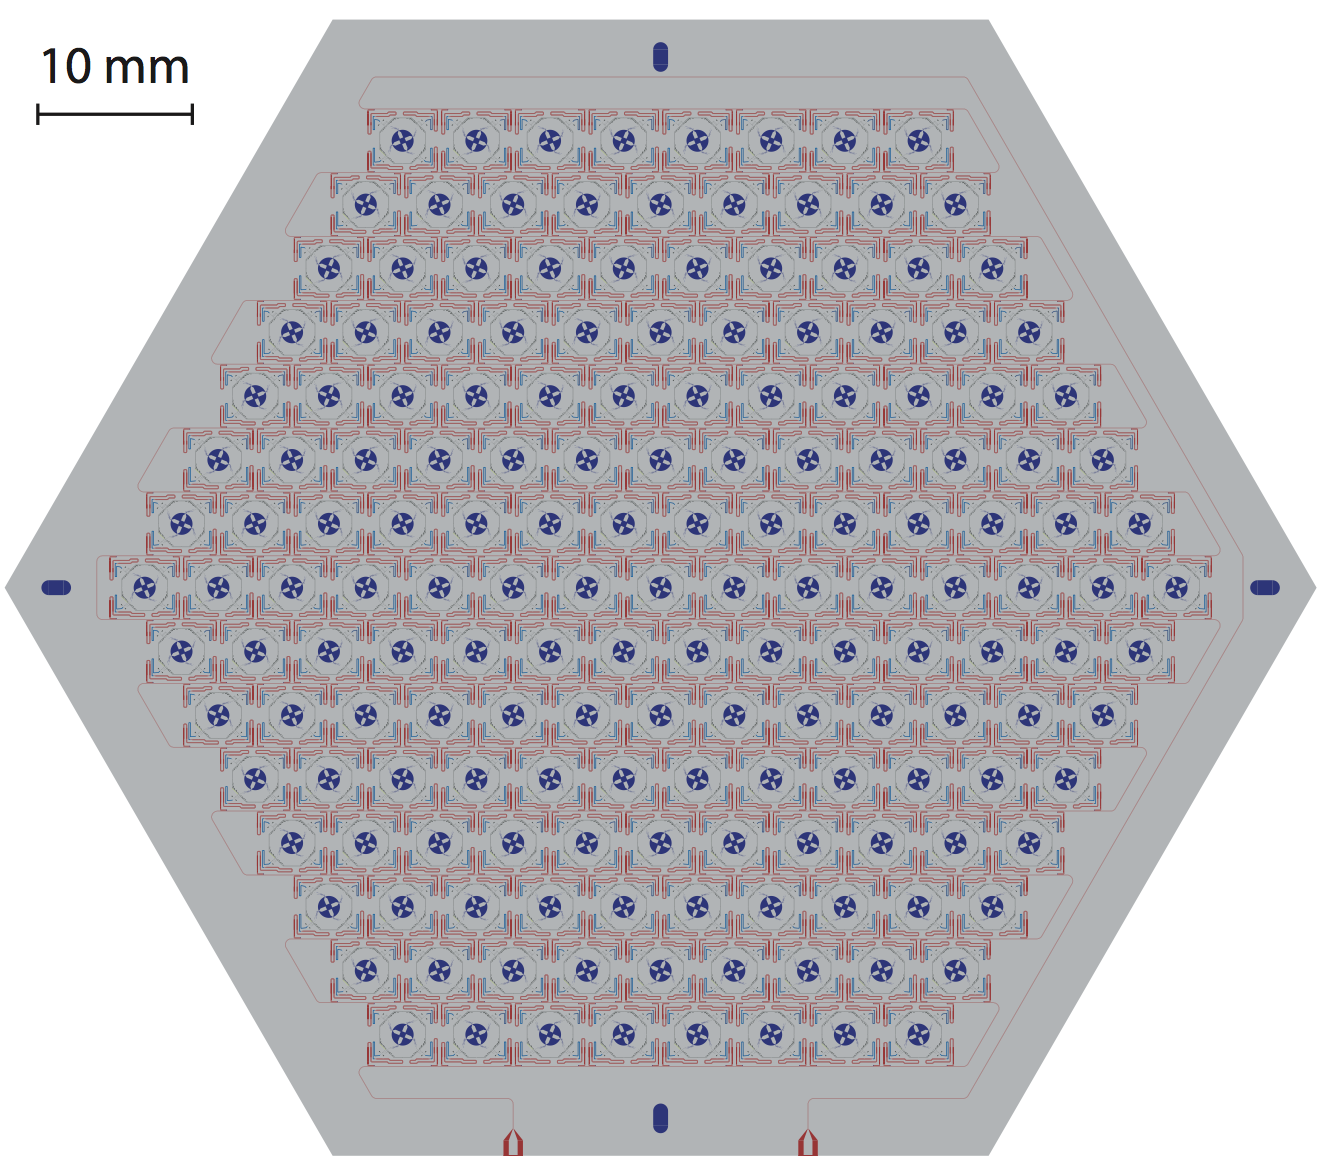
\includegraphics[width=0.8\textwidth]{multichroic/multichroic_hex_array.png}
\caption[A drawing of a prototype 169-pixel multichroic detector array.]
{
A drawing of a prototype 169-pixel multichroic detector array.
}
\label{fig:multichroic_hex_array}
\end{figure}


\begin{appendices}
\chapter{Connections to other work}
\label{chp:connections}

This appendix is intended to facilitate comparison between the results presented here and other works on quasiparticle dynamics.
In a quasiparticle number model like the one used here, all of the dynamical results can be derived from the rate equation for the quasiparticle density.
Table~\ref{tab:connections} summarizes the equivalences between variables that can be inferred by comparing the rate equations given here.
\textcite{Zmuidzinas2012ARCMP} gives for the recombination rate
\begin{equation}
\Gamma_r
  =
  \frac{N_{qp}^2}{2 N^* \tau_\mathrm{max}}
  + \frac{N_{qp}}{\tau_\mathrm{max}},
\end{equation}
where $N_{qp}$ is the quasiparticle number and $N^*$ and $\tau_\mathrm{max}$ are constants.
For bare recombination, \textcite{Wilson2004PRB} give
\begin{equation}
\dv{N}{t}
  =
  2 \left( \Gamma_G - \frac{1}{2} \frac{R}{\mathrm{vol}} N^2 \right),
\end{equation}
where $\Gamma_G$ is the generation \textit{event} rate, $R$ is the recombination constant and $N$ is the number of quasiparticles.
When they include the phonon system, they derive a modified equation that includes an effective recombination constant
$R^* = R / F_\omega$, equivalent to $\qprecombinationeff$ here.
\textcite{Wang2014NatComm} use
\begin{equation}
\dv{x_{qp}}{t}
 =
 -r x_{qp}^2 - s x_{qp} + g,
\end{equation}
where $x_{qp} = n_{qp} / n_{cp}$, $n_{qp}$ is the density of quasiparticles and $n_{cp}$ is the density of Cooper pairs.
The number of Cooper pairs is not given explicitly but can be inferred to be equal to
$n_{cp} = \ssdos \gap_\zerotemp$ in the notation used here
by comparing their expression for the recombination constant $r$ with Equation~\ref{eqn:qprecombination} for $\qprecombinationeff$.
Their solution to their rate equation is equivalent to the solution to Equation~\ref{eqn:rate_qpdensity} given here.
Writing the equation in terms of perturbations to the steady-state density, as is done here, results in a simpler solution and a straightforward treatment of small perturbations.

\begin{table}[tbp]
\centering
\caption
{Connections between notation used in this thesis and in other works.}
\renewcommand{\arraystretch}{1.2}
\begin{tabular}{cccl}
\toprule
This thesis & \textcite{Zmuidzinas2012ARCMP} & \textcite{Wilson2004PRB} & \textcite{Wang2014NatComm} \\
\midrule
$\qprelaxationtime$ & $\tau_\mathrm{qp}$ & $\tau_r^*$ & $\tau_\mathrm{ss}$ \\
$\qprecombinationeff$ & $(2 n^* \tau_\mathrm{max})^{-1}$ & $R^*$ & $n_{cp} r$ \\
$\qpsingledecay$ & $\tau_\mathrm{max}^{-1}$ & $\Gamma_t$ & $s$ \\
$\ssdos$ & $N_0$ & $D(\varepsilon_F) / 2$ &  \\
$\phonontrapping$ &  & $F_\omega$ & $F$ \\
\bottomrule
\end{tabular}
\label{tab:connections}
\end{table}

\chapter{First-order response functions}
\label{chp:first-order_response}

In the approximation scheme introduced by \textcite{Zmuidzinas2012ARCMP} and discussed in Section~\ref{sec:theory.perturbation}, the quasiparticle occupancy $\qpoccupancy(\energy)$ is treated as given.
For calculating the response of a KID, the interesting properties of the superconducting state depend on both the gap and the occupancy; however, the gap also depends on the occupancy and must be determined in a self-consistent manner.
To treat this complication approximately, consider only quantities that are proportional to $\qpoccupancy$, which is used as a small parameter, and write equations that are self-consistent to first order.

For a thermal (Fermi-Dirac) occupancy
$\qpoccupancy(\energy, \temperature) = [\exp(\energy / \kb \temperature) + 1]^{-1}$
at a temperature such that
$\kb \temperature / \gap_\zerotemp \ll 1$,
we can make the approximation
$\qpoccupancy(\energy, \temperature) \approx \exp(-\energy / \kb \temperature)$ as long as there are no states too far below the gap.
This allows the integrals of the first-order quantities to be performed analytically.

\subsubsection{Gap energy}

To derive the first-order response function for the gap, start with the BCS self-consistency equation~\autocite{Tinkham2004}
\begin{equation}
1 
  =
  \bcspotential \sum_{\vwvec} \frac{1 - 2 \qpoccupancy_{\vwvec}}{\left( \blochenergyf_{\vwvec}^2 + \gap^2 \right)^{1/2}},
\end{equation}
where
$\blochenergyf_{\vwvec} = \blochenergy_{\vwvec} - \blochenergy_\fermi$
is the Bloch state energy measured from the Fermi energy $\blochenergy_\fermi$,
and $\qpoccupancy_{\vwvec}$ is the occupancy of the quasiparticle state with energy
$\energy_{\vwvec} = \left( \blochenergyf_{\vwvec}^2 + \gap^2 \right)^{1/2}$.
The sum is over all wavevectors $\vwvec$ such that
\begin{equation}
\left| \blochenergyf_{\vwvec} \right|
  <
  \blochenergyf_\cutoff
  \sim
  \blochenergyf_\debye,
\end{equation}
the Debye energy.
Because $\blochenergy_\debye \gg \gap \gg \kb \temperature$, we have
$\qpoccupancy(\energy = \blochenergyf_\debye) = 0$
and we can take the limits of the corresponding integral to be infinite:
\begin{equation}
1
  =
  \ssdos \ucvolume \bcspotential
  \int_{-\infty}^\infty \dd{\blochenergyf}
  \frac{1 - 2 \qpoccupancy \left(\energy = [\blochenergyf^2 + \gap^2]^{1/2} \right)}{(\blochenergyf^2 + \gap^2)^{1/2}}.
\end{equation}

Expand around the zero-temperature value $\gap_\zerotemp$, using
$\delta\gap = \gap - \gap_\zerotemp$:
\begin{equation}
\frac{1}{(\blochenergyf^2 + \gap^2)^{1/2}}
  =
  \frac{1}{(\blochenergyf^2 + \gap_\zerotemp^2)^{1/2}}
  - \frac{\gap_\zerotemp }{(\blochenergyf^2 + \gap_\zerotemp^2)^{3/2}} \delta\gap
  + \mathcal{O}\left( \delta\gap^2 \right).
\end{equation}
Assume that the occupancy is small so that the term linear in $\qpoccupancy$ is already first-order.
The first-order self-consistency equation is then
\begin{align}
1
  &=
  \ssdos \ucvolume \bcspotential
  \int_{-\infty}^\infty \dd{\blochenergyf}
  \left( \frac{1}{(\blochenergyf^2 + \gap_\zerotemp^2)^{1/2}}
  - \frac{\gap_\zerotemp}{(\blochenergyf^2 + \gap_\zerotemp^2)^{3/2}} \delta\gap
  - \frac{2 \qpoccupancy \left(\energy = [\blochenergyf^2 + \gap_\zerotemp^2]^{1/2} \right)}{(\blochenergyf^2 + \gap_\zerotemp^2)^{1/2}}
  \right) \\
\therefore \qquad
0
  &=
  \delta\gap \int_{-\infty}^\infty \dd{\blochenergyf} \left(
  \frac{\gap_\zerotemp}{(\blochenergyf^2 + \gap_\zerotemp^2)^{3/2}}
 + \frac{2 \qpoccupancy \left(\energy = [\blochenergyf^2 + \gap_\zerotemp^2]^{1/2} \right)}{(\blochenergyf^2 + \gap_\zerotemp^2)^{1/2}}
 \right),
\end{align}
since the left-hand side and the first term define $\gap_\zerotemp$.
With $z = \blochenergyf / \gap_\zerotemp$,
\begin{equation}
\frac{1}{\gap_\zerotemp} \int_{-\infty}^\infty \frac{\dd{z}}{(z^2 + 1)^{3/2}}
  =
  \frac{2}{\gap_\zerotemp},
\end{equation}
so the shift in the gap is
\begin{equation}
\delta\gap
  =
  -\frac{\gap_\zerotemp}{2} \int_{-\infty}^\infty \dd{\blochenergyf}
   \frac{2 \qpoccupancy \left(\energy = [\blochenergyf^2 + \gap_\zerotemp^2]^{1/2} \right)}{(\blochenergyf^2 + \gap_\zerotemp^2)^{1/2}}.
\end{equation}
Use the fact that the integrand is even and change variables to
$\energy = (\blochenergyf^2 + \gap_\zerotemp^2)$:
\begin{equation}
\delta\gap
  =
  - 2 \gap_\zerotemp \int_{\gap_\zerotemp}^\infty \dd{\energy}
   \frac{\qpoccupancy (\energy)}{(\energy^2 - \gap_\zerotemp^2)^{1/2}}.
\end{equation}
Thus, the first-order response function is
\begin{equation}
\responseqpoccupancy_\gap(\energy)
  =
  -\frac{2 \gap_\zerotemp}{(\energy^2 - \gap_\zerotemp^2)^{1/2}}
  =
  -\frac{2 \gap_\zerotemp \qprdos_\zerotemp(\energy)}{\energy},
\label{eqn:first-order_response.responseqpoccupancy_gap}
\end{equation}
where
$\qprdos_\zerotemp = \energy (\energy^2 - \gap_\zerotemp^2)^{-1/2}$
is the reduced density of states at zero temperature.

For a thermal occupancy, using the above low-temperature approximation and the dimensionless variable
$z = \energy / \gap_\zerotemp$,
the first-order shift in the gap is
\begin{align}
\braket{\responseqpoccupancy_\gap}{\qpoccupancy(\temperature)}
  &=
  -2 \gap_\zerotemp \int_{\gap_\zerotemp}^\infty \dd{\energy}
  \frac{\exp(-\energy / \kb \temperature)}{(\energy^2 - \gap_\zerotemp^2)^{1/2}} \\
  &=
  -2 \gap_\zerotemp \int_1^\infty \dd{z} \frac{\exp(-\gap_\zerotemp z / \kb \temperature)}{(z^2 - 1)^{1/2}} \\
  &=
  -2 \gap_\zerotemp K_0 \left( \frac{\gap_\zerotemp}{\kb \temperature} \right),
\label{eqn:first-order_response.responseqpoccupancy_gap_thermal}
\end{align}
where $K_0$ is the zero-order modified Bessel function of the second kind.
\todo[inline]{Replace link when figure is included.}
%Figure~\ref{fig:gap_versus_temperature} shows this expression and the full BCS expression that is also valid at higher temperatures.

\subsubsection{Quasiparticle density}

The first-order response function for the quasiparticle density (or number) follows simply from the definitions.
With the same notation and expanded limits as above,
\begin{equation}
\qpdensity
  =
  2 \ssdos \int_{-\infty}^{\infty} \dd{\blochenergyf}
  \qpoccupancy \left( \energy = (\blochenergyf^2 + \gap^2)^{1/2} \right).
\end{equation}
As above, the integrand is already first-order so we neglect the shift in the gap and set $\gap = \gap_\zerotemp$.
Changing variables and using the symmetry,
\begin{equation}
\qpdensity
  \approx
  \braket{\responseqpoccupancy_{\qpdensity}}{\qpoccupancy}
  =
  \int_{\gap_\zerotemp}^{\infty} \dd{\energy}
  \frac{4 \ssdos \energy}{(\energy^2 - \gap_\zerotemp^2)^{1/2}}
  \qpoccupancy(\energy).
\end{equation}
Including the cutoff in the density of states, the first-order response function is simply
\begin{equation}
\responseqpoccupancy_{\qpdensity}(\energy)
  =
  4 \ssdos \qprdos_\zerotemp(\energy),
\label{eqn:first-order_response.responseqpoccupancy_qpdensity}
\end{equation}
which we would have obtained by naively replacing $\gap$ with $\gap_\zerotemp$ in Equation~\ref{eqn:qpdensity}.

For a thermal occupancy, with the usual approximation, we have
\begin{equation}
\braket{\responseqpoccupancy_{\qpdensity}}{\qpoccupancy(\temperature)}
  =
  4 \ssdos \int_{\gap_\zerotemp}^{\infty} \dd{\energy}
  \frac{\energy \exp(-\energy / \kb \temperature)}{(\energy^2 - \gap_\zerotemp^2)^{1/2}}.
\end{equation}
\todo[inline]{Flesh out using Abramowitz and Stegun}
This integral is done by \textcite{Thomas2015SUST}, who give
\begin{equation}
\qpdensity(\temperature)
  =
  4 \ssdos \gap_\zerotemp
  K_1(\gap_\zerotemp / \kb \temperature)
  \approx
  4 \ssdos \gap_\zerotemp
  \left( \frac{\pi \kb \temperature}{2 \gap_\zerotemp} \right)^{1/2}
  \exp \left( -\frac{\gap_\zerotemp}{\kb \temperature} \right),
\label{eqn:first-order_response.qpdensity_thermal}
\end{equation}
which is Equation~\ref{eqn:qpdensity_thermal} in the main text.

\subsubsection{Complex conductivity}

\begin{figure}[htb]
\centering
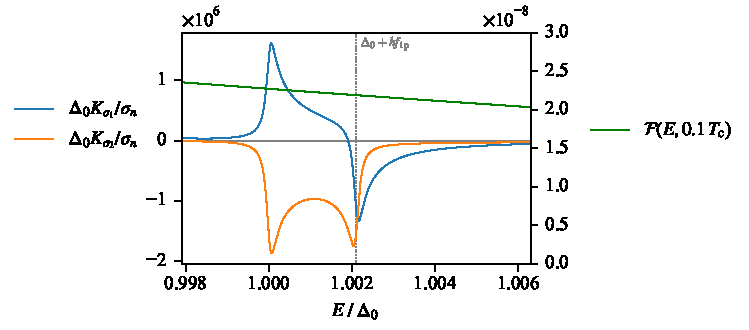
\includegraphics[width=\textwidth]{first-order_response/responseqpoccupancy_conductivity_f_1p.pdf}
\caption
[The first-order response functions for the real and imaginary parts of the conductivity at $\freadout_\singlepol$.]
{The first-order response functions for the real and imaginary parts of the conductivity at $\freadout_\singlepol = \SI{0.1}{GHz}$ versus energy in units of the gap, and a thermal occupancy.
The left axis shows Equations~\ref{eqn:responseqpoccupancy_reconductivity} and~\ref{eqn:responseqpoccupancy_imconductivity} multiplied by constants to make them dimensionless.
For display, the density of states factors have been broadened using $\mitrovic / \gap_\zerotemp = 0.0002$.
The right axis shows a thermal occupancy at a typical KID operating temperature.
Figure~\ref{fig:responseqpoccupancy_conductivity_f_mc} shows the same quantities at a much higher frequency, where the peaks in the response functions are farther apart.}
\label{fig:responseqpoccupancy_conductivity_f_1p}
\end{figure}

In calculating the first-order response functions for the complex conductivity at the readout frequency $\freadout$ we can assume that $\planck \freadout / 2 \gap \ll 1$.
The expressions for $\responseqpoccupancy_{\reconductivity}$ and $\responseqpoccupancy_{\imconductivity}$ are plotted for two different frequencies in Figures~\ref{fig:responseqpoccupancy_conductivity_f_mc} and~\ref{fig:responseqpoccupancy_conductivity_f_1p}.

For the real part of the conductivity, start with Equation~\ref{eqn:mattisbardeen1}.
In this limit, only the first term is present:
\begin{equation}
\frac{\reconductivity(\freadout)}{\normalconductivity}
  =
  \frac{2}{\planck \freadout} \int_\gap^\infty \dd{\energy}
  \left[ \qpoccupancy(\energy) - \qpoccupancy(\energy + \planck \freadout) \right]
  \frac{\energy^2 + \gap^2 + \planck \freadout \energy}
  {[\energy^2 - \gap^2]^{1/2} [(\energy + \planck \freadout)^2 - \gap^2]^{1/2}}.
\label{eqn:mattisbardeen1subgap}
\end{equation}
For brevity, and to anticipate possible broadening, rewrite the integrand using the density of states:
\begin{equation}
\frac{\reconductivity(\freadout)}{\normalconductivity}
  =
  \frac{2}{\planck \freadout} \int_\gap^\infty \dd{\energy}
  \left[ \qpoccupancy(\energy) - \qpoccupancy(\energy + \planck \freadout) \right]
  \qprdos(\energy) \qprdos(\energy + \planck \freadout)
  \left(1 + \frac{\gap^2}{\energy (\energy + \planck \freadout)} \right).
\end{equation}
The entire integrand is proportional to the occupancy, so
$\reconductivity(\temperature = 0) = 0$
and we may neglect the first-order shift in the gap, which would appear at second order, and set
$\gap = \gap_\zerotemp$.
If we write the density of states in the form
$\qprdos_\zerotemp(\energy) = \Re{\energy (\energy^2 - \gap_\zerotemp^2)^{-1/2}}$,
we can change variables in the second term and combine the integrals, setting both lower limits to 0:
\begin{align}
\begin{split}
\frac{\reconductivity(\freadout)}{\normalconductivity}
  &=
  \frac{2}{\planck \freadout} \int_0^\infty \dd{\energy}
  \qpoccupancy(\energy)
  \bigg[
  \qprdos_\zerotemp(\energy) \qprdos_\zerotemp(\energy + \planck \freadout)
  \left(1 + \frac{\gap_\zerotemp^2}{\energy (\energy + \planck \freadout)} \right) \\
  &\hspace{1.3in} - \qprdos_\zerotemp(\energy - \planck \freadout) \qprdos_\zerotemp(\energy)
  \left(1 + \frac{\gap_\zerotemp^2}{(\energy - \planck \freadout) \energy} \right)
  \bigg].
\end{split}
\end{align}
(This change of variables should not cause problems unless there are states far below the gap, close to $\energy = 0$.)
We can now read off the first-order response function:
\begin{equation}
\responseqpoccupancy_{\reconductivity}(\energy)
  =
  \frac{2 \normalconductivity \qprdos_\zerotemp(\energy)}{\planck \freadout}
  \left[
  \qprdos_\zerotemp(\energy + \planck \freadout)
  \left(1 + \frac{\gap_\zerotemp^2}{\energy (\energy + \planck \freadout)} \right)
  - \qprdos_\zerotemp(\energy - \planck \freadout)
  \left(1 + \frac{\gap_\zerotemp^2}{(\energy - \planck \freadout) \energy} \right)
  \right],
\label{eqn:first-order_response.responseqpoccupancy_reconductivity}
\end{equation}
which matches Equation~\ref{eqn:responseqpoccupancy_reconductivity}.
To calculate $\braket{\responseqpoccupancy_{\reconductivity}}{\qpoccupancy(\temperature)}$ for a thermal occupancy  $\qpoccupancy(\temperature)$ at low temperature, start from Equation~\ref{eqn:mattisbardeen1subgap}, and, following \textcite{Barends2009}, change to a dimensionless variable
\begin{equation}
z
  =
  \frac{2}{\planck \freadout} \left( \energy - \gap_\zerotemp + \frac{\planck \freadout}{2} \right).
\end{equation}
Then, using
$D = 2 \gap_\zerotemp / \planck \freadout \gg 1$
so that
$\energy = (\planck \freadout / 2) (z + D - 1)$,
\begin{align}
\begin{split}
\frac{\braket{\responseqpoccupancy_{\reconductivity}}{\qpoccupancy(\temperature)}}{\normalconductivity}
  &=
  2 \sinh \left( \frac{\planck \freadout}{2 \kb \temperature} \right)
  \exp \left( -\frac{\gap_\zerotemp}{\kb \temperature} \right)
  \int_1^\infty
  \exp \left( -\frac{\planck \freadout z}{2 \kb \temperature} \right) \\
  &\hspace{1in} \times  \frac{z^2 + 2 D z + 2 D^2 - 1}{[2 D (z - 1) + (z - 1)^2]^{1/2} [2 D (z + 1) + (z + 1)^2]^{1/2}} \dd{z} \\
  &\approx
  2 \sinh \left( \frac{\planck \freadout}{2 \kb \temperature} \right)
  \exp \left( -\frac{\gap_\zerotemp}{\kb \temperature} \right)
  \int_1^\infty
  \exp \left( -\frac{\planck \freadout z}{2 \kb \temperature} \right)
  \frac{D}
  {(z - 1)^{1/2} (z + 1)^{1/2}} \dd{z}.
\end{split}
\end{align}
The exponential falls off rapidly, so the weight is highest near $z \gtrsim 1$.
We thus neglect all terms in the numerator except $2 D^2$.
In the denominator, $(z - 1)^2$ is negligible near $z = 1$ where the weight is highest.
For $z \approx 2 D$, where $(z \pm 1)^2$ becomes significant, the argument of the exponential is negative and large
$(2 \gap_\zerotemp / \kb \temperature \gg 1)$, so we can also neglect these terms.
In this form, the integral can be done analytically, as above, with the result
\begin{equation}
\frac{\braket{\responseqpoccupancy_{\reconductivity}}{\qpoccupancy(\temperature)}}{\normalconductivity}
  =
  \frac{4 \gap_\zerotemp}{\planck \freadout}
  \exp \left( -\frac{\gap_\zerotemp}{\kb \temperature} \right)
  \sinh \left( \frac{\planck \freadout}{2 \kb \temperature} \right)
  K_0 \left( \frac{\planck \freadout}{2 \kb \temperature} \right).
\label{eqn:first-order_response.responseqpoccupancy_reconductivity_thermal}
\end{equation}

The derivation of the first-order response function for the imaginary part of the conductivity proceeds similarly, starting from Equation~\ref{eqn:mattisbardeen2} with the lower bound appropriate for
$\planck \freadout / 2 \gap < 1$:
\begin{equation}
\frac{\imconductivity}{\normalconductivity}
  =
  \frac{1}{\planck \freadout} \int_{\gap - \planck \freadout}^{\gap} \dd{\energy}
  \left[ 1 - 2 \qpoccupancy(\energy + \planck \freadout) \right]
  \frac{\energy (\energy + \planck \freadout) + \gap^2}
  {[\gap^2 - \energy^2]^{1/2} [(\energy + \planck \freadout)^2 - \gap^2]^{1/2}}.
\label{eqn:mattisbardeen2subgap}
\end{equation}
The occupancy does not appear in the first term, so the zero-temperature value is nonzero.
Using the same dimensionless variables as above,
\begin{align}
\begin{split}
\frac{\imconductivity(\temperature = 0)}{\normalconductivity}
  &=
  \int_{-1}^{1} \frac{\dd{z}}{2}
  \frac{z^2 + 2 D z + 2 D^2 - 1}{[2 D (1 - z) - (1 - z)^2]^{1/2} [2 D (1 + z) + (1 + z)^2]^{1/2}} \\
  &\approx
  \int_{-1}^{1} \dd{z}
  \frac{D / 2}{(1 - z)^{1/2} (1 + z)^{1/2}}.
\end{split}
\end{align}
As before, we retain only the largest term in the numerator.
The integrand is singular at both limits, and we neglect
$(z \pm 1)^2$
in the denominator because the other terms dominate near the limits.
\todo[inline]{Flesh out using A\&S.}
With the substitution $\theta = \arccos(-z)$, we obtain
\begin{equation}
\frac{\imconductivity(\temperature = 0)}{\normalconductivity}
  =
  \frac{\pi \gap_\zerotemp}{\planck \freadout}.
\end{equation}
The second term in Equation~\ref{eqn:mattisbardeen2subgap} is linear in $\qpoccupancy$, so again we set $\gap = \gap_\zerotemp$ in this term.
However, the first term also produces a first-order contribution because the shift in the gap appears at this order:
$\gap = \gap_\zerotemp + \braket{\responseqpoccupancy_{\gap}}{\qpoccupancy}$.
Using Equation~\ref{eqn:first-order_response.responseqpoccupancy_gap}, factoring the second term, and changing limits gives
\begin{align}
\begin{split}
\frac{\imconductivity - \imconductivity(\temperature = 0)}{\normalconductivity}
  &=
\frac{\pi \braket{\responseqpoccupancy_{\gap}}{\qpoccupancy}}{\planck \freadout}
  - \frac{2}{\planck \freadout} \int_{\gap}^{\gap + \planck \freadout} \dd{\energy}
  \qpoccupancy(\energy)
  \frac{(\energy - \planck \freadout) \energy + \gap^2}
  {[\gap^2 - (\energy - \planck \freadout)^2]^{1/2} [\energy^2 - \gap^2]^{1/2}} \\
  &=
  \int_{0}^{\infty}
  \dd{\energy} \qpoccupancy(\energy)
  \left( -\frac{2 \pi \gap_\zerotemp \qprdos_\zerotemp(\energy)}{\planck \freadout \energy} \right) \\
  &\quad
  + \int_{0}^{\infty} \dd{\energy} \qpoccupancy(\energy)
  \left( -\frac{2 \qprdos_\zerotemp(\energy)}{\planck \freadout} \right)
  \left( 1 + \frac{\gap_\zerotemp^2}{\energy (\energy - \planck \freadout)} \right) \\
  &\hspace{1in} \times
  \frac{\stepfunction(\gap_\zerotemp + \planck \freadout - \energy) (\energy - \planck \freadout)}{[\gap_\zerotemp^2 - (\energy - \planck \freadout)^2]^{1/2}},
\end{split}
\end{align}
where $\stepfunction$ is the unit step function, which produces the cutoff at the upper limit.
In both integrals, the cutoff at the appropriate lower limit is 
presumably determined by the density of states.
The singularity at $\energy = \gap_\zerotemp + \planck \freadout$ can be broadened in a non-rigorous way by replacing the final fraction containing the step function with
\begin{equation}
\mathrm{Re}  \left[
  \frac{\energy - \planck \freadout}{[\gap_\zerotemp^2 - (\energy - \planck \freadout)^2]^{1/2}} \right],
\end{equation}
as was done for display in the figures.
The response function is thus
\begin{equation}
\responseqpoccupancy_{\imconductivity}(\energy)
  =
  - \frac{2 \normalconductivity \qprdos_\zerotemp(\energy)}{\planck \freadout}
  \left[
  \frac{\pi \gap_\zerotemp}{\energy}
  +   \left( 1 + \frac{\gap_\zerotemp^2}{\energy (\energy - \planck \freadout)} \right)
  \frac{\stepfunction(\gap_\zerotemp + \planck \freadout - \energy) (\energy - \planck \freadout)}{[\gap_\zerotemp^2 - (\energy - \planck \freadout)^2]^{1/2}}
  \right],
\label{eqn:first-order_response.responseqpoccupancy_imconductivity}
\end{equation}
matching Equation~\ref{eqn:responseqpoccupancy_imconductivity}.
For a thermal occupancy, we make the usual approximation.
The first term involves the integral for the gap shift, given by Equation~\ref{eqn:first-order_response.responseqpoccupancy_gap_thermal}.
In the second term, start with Equation~\ref{eqn:mattisbardeen2subgap}, and set $\gap = \gap_\zerotemp$:
\begin{align}
\begin{split}
\frac{\braket{\responseqpoccupancy_{\imconductivity}}{\qpoccupancy(\temperature)}}{\normalconductivity}
  &=
  \frac{\pi \braket{\responseqpoccupancy_{\gap}}{\qpoccupancy(\temperature)}}{\planck \freadout} \\
  &\quad
  - \frac{2}{\planck \freadout} \int_{\gap_\zerotemp - \planck \freadout}^{\gap_\zerotemp} \dd{\energy}
  \frac{\exp(-[\energy + \planck \freadout] / \kb \temperature) \; (\energy (\energy + \planck \freadout) + \gap_\zerotemp^2)}
  {[\gap_\zerotemp^2 - \energy^2]^{1/2} [(\energy + \planck \freadout)^2 - \gap_\zerotemp^2]^{1/2}}.
\end{split}
\end{align}
Use the same dimensionless variables as above and make the same approximations:
\begin{align}
\begin{split}
\frac{\braket{\responseqpoccupancy_{\imconductivity}}{\qpoccupancy(\temperature)}}{\normalconductivity}
  &=
  -\frac{2 \pi \gap_\zerotemp}{\planck \freadout}
  K_0 \left( \frac{\gap_\zerotemp}{\kb \temperature} \right) \\
  &\quad
  - \exp \left( -\frac{\gap_\zerotemp}{\kb \temperature} \right)
  \exp \left( -\frac{\planck \freadout}{2 \kb \temperature} \right) \\
  &\qquad \times
  \int_{-1}^{1} \dd{z}
  \frac{\exp \left( -\planck \freadout z / 2 \kb \temperature \right) \; (z^2 + 2 D z + 2 D^2 - 1)}{[2 D (1 - z) - (1 - z)^2]^{1/2} [2 D (1 + z) + (1 + z)^2]^{1/2}} \\
  &\approx
  -\frac{2 \pi \gap_\zerotemp}{\planck \freadout}
  K_0 \left( \frac{\gap_\zerotemp}{\kb \temperature} \right) \\
  &\quad - \exp \left( -\frac{\gap_\zerotemp}{\kb \temperature} \right)
  \exp \left( -\frac{\planck \freadout}{2 \kb \temperature} \right)
  \int_{-1}^{1} \dd{z}
  \frac{D \exp \left( -\planck \freadout z / 2 \kb \temperature \right)}{(1 - z)^{1/2} (1 + z)^{1/2}}.
\end{split}
\end{align}
\todo[inline]{Compare this to the mathworld form.}
Using $\theta = \arccos(-z)$ and
\begin{equation}
I_0(a)
  = \frac{1}{\pi} \int_{0}^{\pi} \dd{\theta} \exp [a \cos(\theta)],
\end{equation}
where $I_0$ is the zero-order modified Bessel function of the first kind, we obtain
\begin{equation}
\frac{\braket{\responseqpoccupancy_{\imconductivity}}{\qpoccupancy(\temperature)}}{\normalconductivity}
  =
  -\frac{2 \pi \gap_\zerotemp}{\planck \freadout}
  \left[
  K_0 \left( \frac{\gap_\zerotemp}{\kb \temperature} \right)
  + \exp \left( -\frac{\gap_\zerotemp}{\kb \temperature} \right)
  \exp \left( -\frac{\planck \freadout}{2 \kb \temperature} \right)
  I_0 \left( \frac{\planck \freadout}{2 \kb \temperature} \right)
  \right],
\label{eqn:first-order_response.responseqpoccupancy_imconductivity_thermal}
\end{equation}
matching Equation~\ref{eqn:responseqpoccupancy_imconductivity_thermal}.

\chapter{Hardware}
\label{chp:hardware}

\section{KID readout}
\label{sec:hardware.kid_readout}

\begin{figure}[ht]
\centering
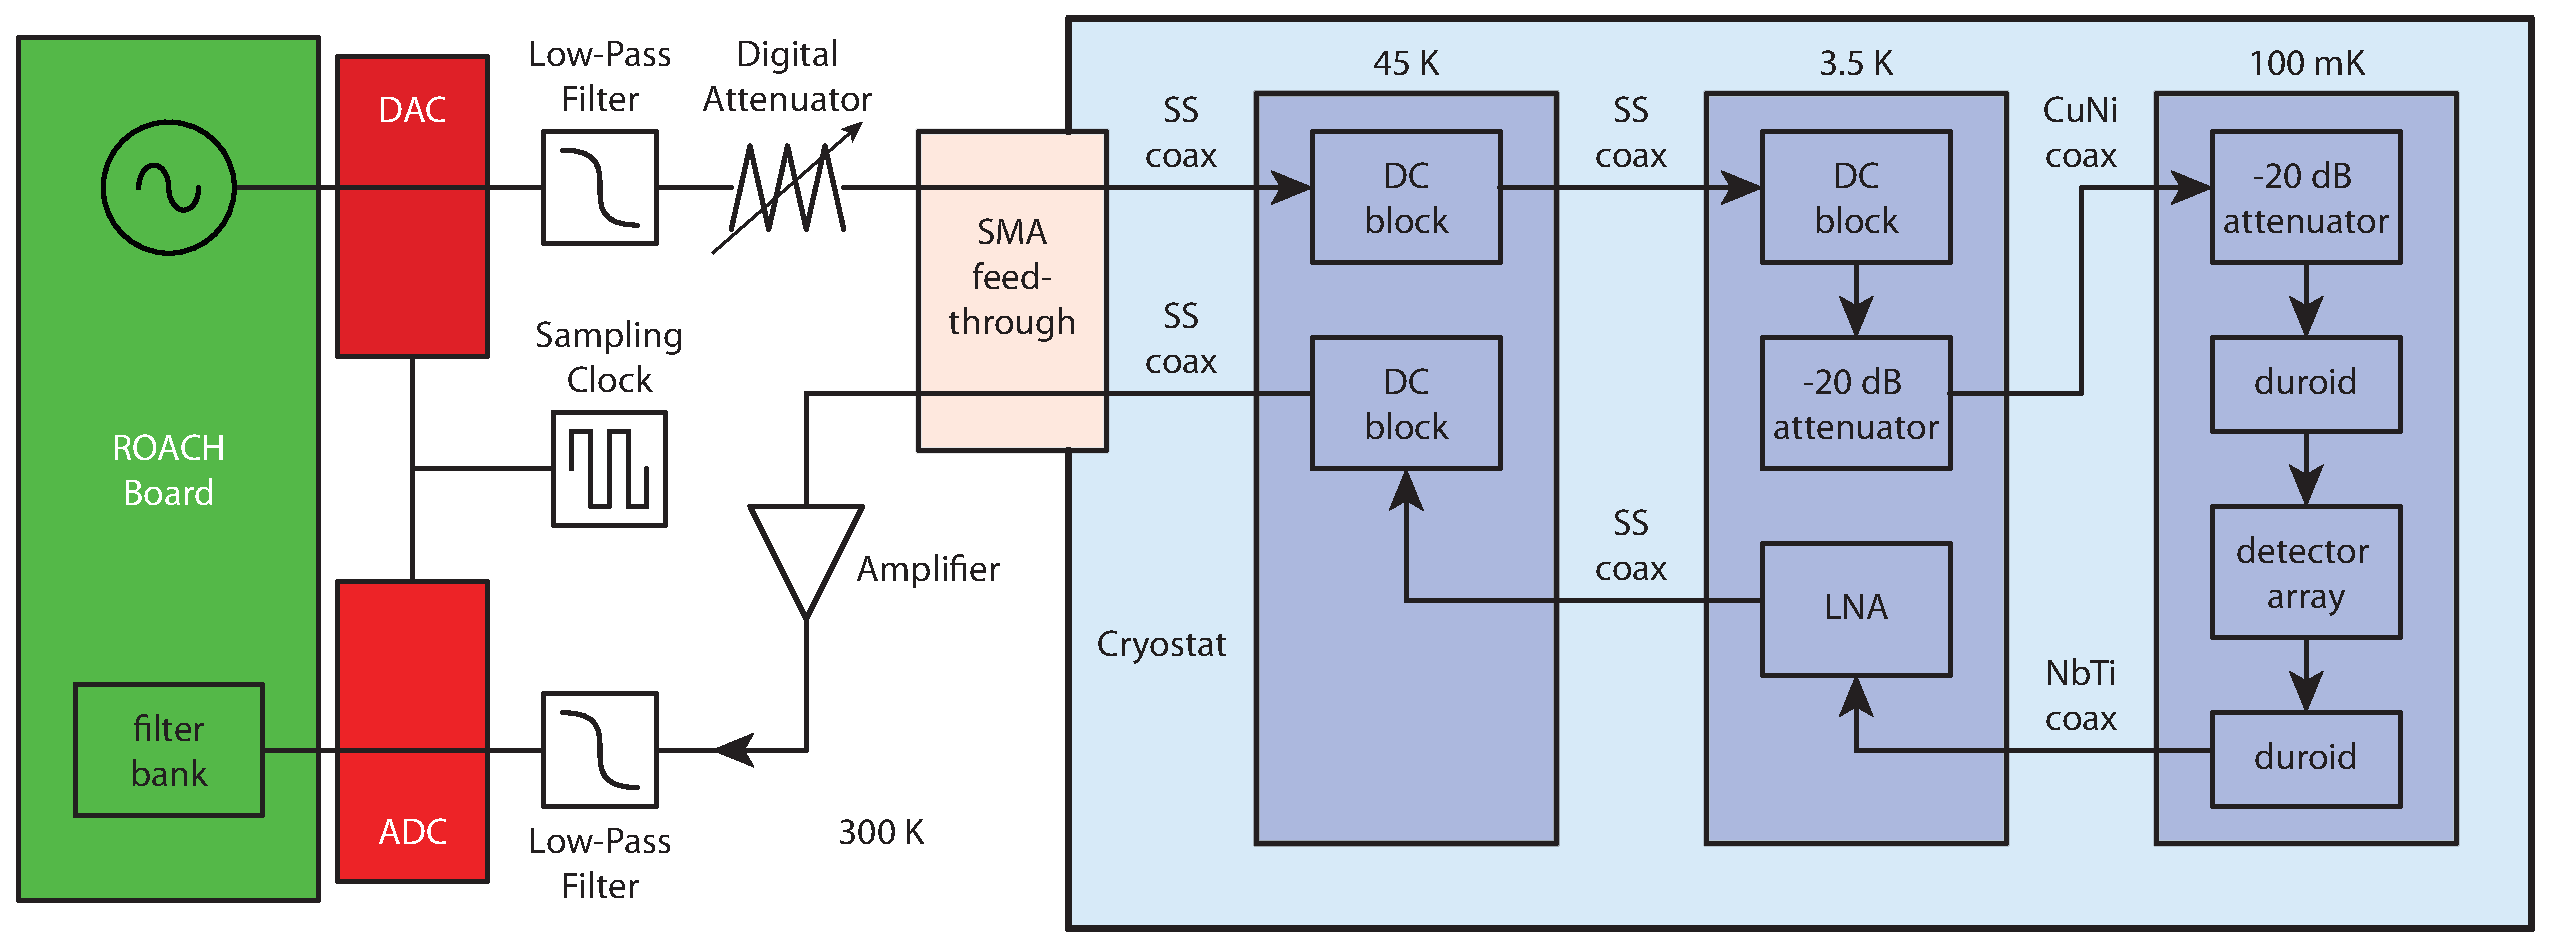
\includegraphics[width=0.8\textwidth]{hardware/baseband_readout_schematic.pdf}
\caption[A schematic of the ROACH-1 baseband readout system, including components in the cryostat.]
{
A schematic of the ROACH-1 baseband readout system, including components in the cryostat.
This system is capable of measuring resonances below approximately \SI{200}{MHz}.
This figure was published in \textcite{McCarrick2014RSI}.
}
\label{fig:baseband_readout_schematic}
\end{figure}

\begin{figure}[htb]
\centering
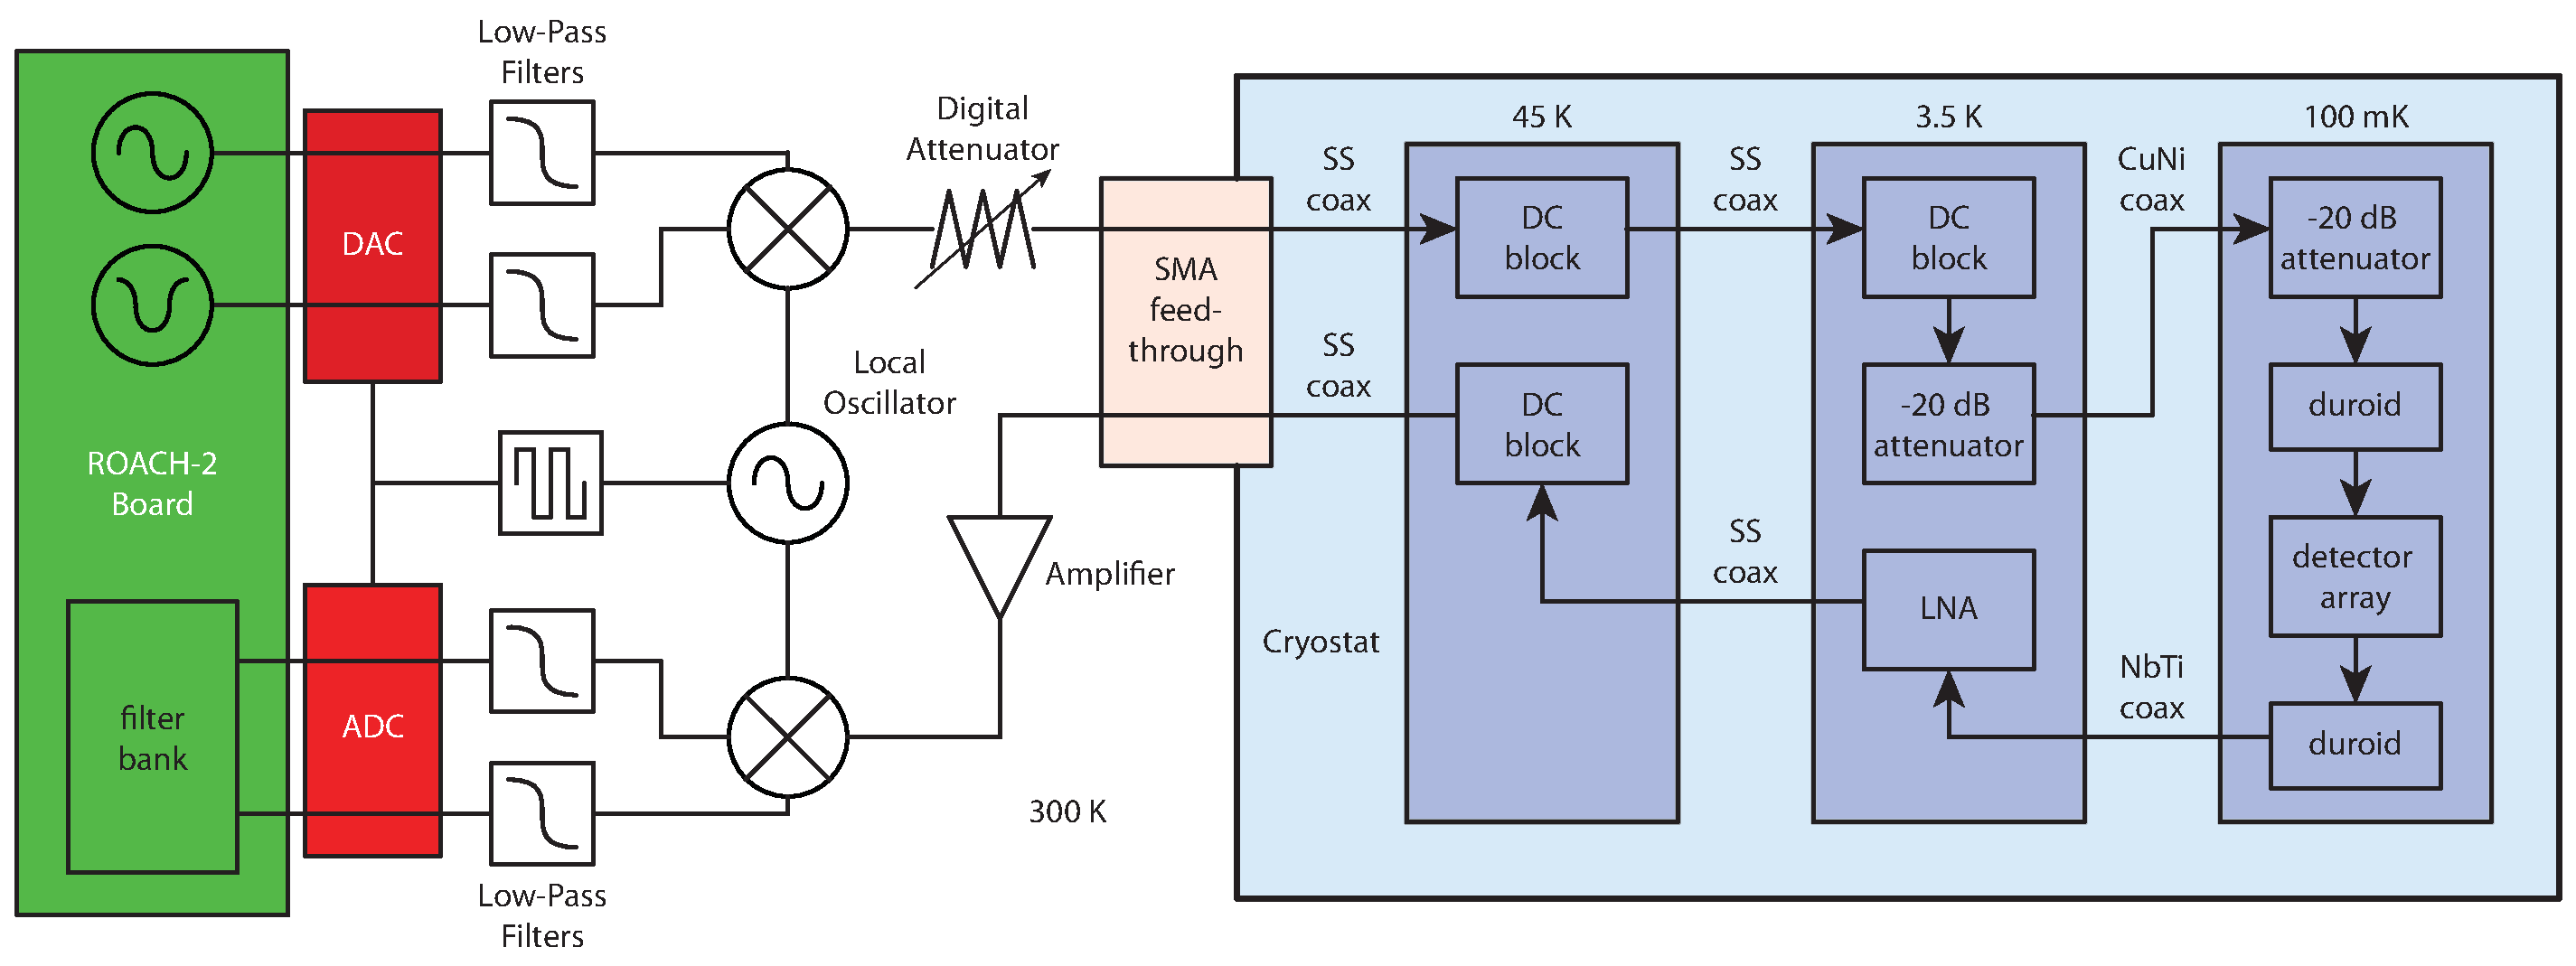
\includegraphics[width=0.8\textwidth]{hardware/heterodyne_readout_schematic.pdf}
\caption[A schematic of the ROACH-2 heterodyne readout system, including components in the cryostat.]
{
A schematic of the ROACH-2 heterodyne readout system, including components in the cryostat.
This system is capable of measuring resonances between approximately \SIrange{700}{4000}{MHz}.
This figure was published in \textcite{Johnson2016SPIE}.
}
\label{fig:heterodyne_readout_schematic}
\end{figure}

\begin{figure}[htb]
\centering
\includegraphics[width=\textwidth]{hardware/roach-2_v2.pdf}
\caption[Photographs of the ROACH-2 board and the heterodyne analog electronics box.]
{
\textbf{(Left)}
A photograph of the ROACH-2 board.
\textbf{(Right)}
A photograph of the analog electronics box for the heterodyne readout system, including the local oscillator (LO).
This figure was published in \textcite{Johnson2016SPIE}.
}
\label{fig:roach-2_v2}
\end{figure}

\clearpage


\section{Millimeter-wave source}
\label{sec:hardware.mmw_source}

\begin{table}[htb]
\centering
\caption[Primary components of the millimeter-wave source.]{Primary components of the millimeter-wave source.
The terminator and amplifiers are built-in components, but are used only in broadband mode, in which they produce broadband noise.
In continuous-wave mode, we instead use an external microwave signal generator that feeds the input to the PIN switch.}
\renewcommand{\arraystretch}{1.2}
\begin{tabular}{lll}
\toprule
\textbf{Component} & \textbf{Vendor} & \textbf{Part Number} \\
\midrule
50~$\Omega$ terminator & Minicircuits & ANNE-50X \\ 
High gain amplifiers & Spacek Labs & SG134-40-17 \\ 
PIN switch & Narda & S213D \\ 
Active multiplier & Millitech & AMC-05 \\
Variable attenuators & Custom Microwave & VA6R \\
Band-pass filter & Pacific Millimeter & 14020 \\
Directional coupler & Millitech & CL3-006 \\
Zero-bias diode power detector & Virginia Diodes, Inc. & WR6.5-ZBD \\
\bottomrule
\end{tabular}
\label{tab:mmw_source}
\end{table}

\begin{figure}[htb]
\centering
\includegraphics[width=0.7\textwidth]{hardware/millimeter-wave_source_annotated.png}
\caption[A photograph of the electronic millimeter-wave source.]
{
A photograph of the electronic millimeter-wave source.
}
\label{fig:millimeter-wave_source_annotated}
\end{figure}

\clearpage

\begin{comment}
\section{Package for multichroic detectors}
\label{sec:hardware.package}

\todo[inline]{Describe the multichroic detector package.}
The upper piece, the \textit{holder}, includes the feedhorns and waveguides, structures used to align the wafer, and 
The lower piece, the \textit{lid}, closes the module and contains backshorts that improve the millimeter-wave coupling.

\begin{figure}[htb]
\centering
\missingfigure[figwidth=\textwidth]{Lots of pictures of the multichroic package.}
\caption[Pictures of the multichroic package.]
{Pictures of the multichroic package.}
\label{fig:multichroic_package}
\end{figure}

\clearpage
\end{comment}

\section{Cryostat}
\label{sec:hardware.cryostat}

\begin{figure}[htb]
\centering
\includegraphics[height=0.7\textheight]{hardware/starcryo_cryostat_with_hwp.jpg}
\caption[The interior of a cryostat used for detector testing, in its ``half-wave plate'' configuration.]
{
The interior of a cryostat used for detector testing, in its ``half-wave plate'' configuration.
Light from an electronic millimeter-wave source propagates down the rectangular waveguide and exits the feed horn.
The cryogenic half-wave plate may rotate the polarization axis.
The motor rotates the half-wave plate.
The Eccosorb slab is nearly opaque and provides a beam-filling black body load with a temperature that can be controlled using the heater.
This configuration is similar to that used for the optical testing of detectors described in Section~\ref{sec:multichroic.mkidarray02}.
}
\label{fig:starcryo_cryostat_with_hwp}
\end{figure}

\begin{figure}[ht]
\centering
\includegraphics[height=0.8\textheight]{hardware/starcryo_cryostat_with_optics_box.jpg}
\caption[The interior of a cryostat used for detector testing, in its ``optics box'' configuration.]
{
The interior of a cryostat used for detector testing, in its ``optics box'' configuration.
Light from an electronic millimeter-wave source propagates down the rectangular waveguide and exits the feed horn.
The optics box contains mirrors (not visible) that convert the horn beam into a plane wave that illuminates the top of the detector package.
The Eccosorb slab is nearly opaque and provides a beam-filling black body load with a temperature that can be controlled using the heater.
The experiment described in Section~\ref{sec:sensitivity.measuring} used a similar configuration to that shown here.
The experiment described in Section~\ref{sec:loss.vortex} was performed with the package attached to the \SI{0.1}{K}, as shown here, but the optics box was removed and the magnet array was placed beneath the package, outside the cryostat shells that have been removed for this photograph.
}
\label{fig:starcryo_cryostat_with_optics_box}
\end{figure}


\end{appendices}

\clearpage
\phantomsection
\addcontentsline{toc}{chapter}{References}
\singlespacing
\printbibliography[title={References}]

% Three blank pages added for printing to produce one blank sheet at the end
\blankpage
\blankpage
\blankpage

\end{document}
